%%%%%%%%%%%%%%%%%%%%%%%%%%%%%%%%%%%%%%%%%
% The Legrand Orange Book
% LaTeX Template
% Version 2.0 (9/2/15)
%
% This template has been downloaded from:
% http://www.LaTeXTemplates.com
%
% Mathias Legrand (legrand.mathias@gmail.com) with modifications by:
% Vel (vel@latextemplates.com)
%
% License:
% CC BY-NC-SA 3.0 (http://creativecommons.org/licenses/by-nc-sa/3.0/)
%
% Compiling this template:
% This template uses biber for its bibliography and makeindex for its index.
% When you first open the template, compile it from the command line with the 
% commands below to make sure your LaTeX distribution is configured correctly:
%
% 1) pdflatex main
% 2) makeindex main.idx -s StyleInd.ist
% 3) biber main
% 4) pdflatex main x 2
%
% After this, when you wish to update the bibliography/index use the appropriate
% command above and make sure to compile with pdflatex several times 
% afterwards to propagate your changes to the document.
%
% This template also uses a number of packages which may need to be
% updated to the newest versions for the template to compile. It is strongly
% recommended you update your LaTeX distribution if you have any
% compilation errors.
%
% Important note:
% Chapter heading images should have a 2:1 width:height ratio,
% e.g. 920px width and 460px height.
%
%%%%%%%%%%%%%%%%%%%%%%%%%%%%%%%%%%%%%%%%%

%----------------------------------------------------------------------------------------
%	PACKAGES AND OTHER DOCUMENT CONFIGURATIONS
%----------------------------------------------------------------------------------------

\documentclass[11pt,fleqn]{book} % Default font size and left-justified equations

\usepackage{float}% para ter [H]
\usepackage{fancyvrb}

%----------------------------------------------------------------------------------------
%	DATOS DEL LIBRO
%----------------------------------------------------------------------------------------
\newcommand{\mytitle}[0]{ Samba de Gafieira }
\newcommand{\mysubtitle}[0]{ Dan{\c{c}}a e Partitura de Movimento}
\newcommand{\myauthor}[0]{ Fernando Pujaico Rivera}
%----------------------------------------------------------------------------------------
\newcommand{\imprimirlocal}[0]{Brasil}
\newcommand{\imprimiryear}[0]{XXXXXXXXXXX}
\newcommand{\imprimirdata}[0]{9 de abril do \imprimiryear}
\newcommand{\imprimirtipotrabalho}[0]{Bibliografia}
\newcommand{\imprimirsize}[0]{16x30cm}
\newcommand{\imprimirisbn}[0]{XXXXXXXXXXX}
\newcommand{\imprimireditora}[0]{Editora XXXXXXXXXXX}
%----------------------------------------------------------------------------------------
\newcommand{\ImprimirLinkHomePageLivro}[0]{\url{http://XXXXXXXXXXX.com}}
\newcommand{\ImprimirLinkCompraLivroImpresso}[0]{\url{http://XXXXXXXXXXX.com/comprarfisico/}}
\newcommand{\ImprimirLinkCompraLivroDigital}[0]{\url{http://XXXXXXXXXXX.com/comprardigital/}}
%----------------------------------------------------------------------------------------
\newcommand{\ImprimirEmail}[0]{ \href{mailto:fernando.pujaico.rivera@gmail.com}{fernando.pujaico.rivera@gmail.com}}
%----------------------------------------------------------------------------------------

%----------------------------------------------------------------------------------------



%----------------------------------------------------------------------------------------
%	XCOLOR
%----------------------------------------------------------------------------------------
\usepackage[dvipsnames*,svgnames]{xcolor}
\definecolor{colorlowgray}{RGB}{240,240,240}
\definecolor{colorsystemdefault}{RGB}{16,81,15} % Define the color used for highlighting throughout the book
\definecolor{colormylink}{RGB}{16,120,15} % Define the 

%----------------------------------------------------------------------------------------
%	COLOR
%----------------------------------------------------------------------------------------
\usepackage{color}
\definecolor{colorlowred}{rgb}{0.98,0.88,0.82}
%\definecolor{colordarkgray}{rgb}{0.5,0.5,0.5}
%\definecolor{colormauve}{rgb}{0.58,0,0.82}

%----------------------------------------------------------------------------------------


%----------------------------------------------------------------------------------------
%	VARIOUS REQUIRED PACKAGES AND CONFIGURATIONS
%----------------------------------------------------------------------------------------

\usepackage[top=3cm,bottom=3cm,left=3cm,right=3cm,headsep=10pt,a4paper]{geometry} % Page margins

\usepackage{graphicx} % Required for including pictures
\graphicspath{{pictures/}} % Specifies the directory where pictures are stored

\usepackage{lipsum} % Inserts dummy text

\usepackage[brazil]{babel}
%\usepackage[english]{babel} % English language/hyphenation

%----------------------------------------------------------------------------------------
%	Footnote
%----------------------------------------------------------------------------------------
\usepackage{scrextend} %multiple reference

%----------------------------------------------------------------------------------------
% Page counter
%----------------------------------------------------------------------------------------
\usepackage{lastpage}

%----------------------------------------------------------------------------------------
% GLOSSARIO
%----------------------------------------------------------------------------------------
\usepackage{nomencl}


%----------------------------------------------------------------------------------------
% Par diferentes modelos de caption.
%----------------------------------------------------------------------------------------
\usepackage{caption}
\usepackage{subcaption}
%\usepackage{wrapfig}

%----------------------------------------------------------------------------------------
% Para \singlespacing 
%----------------------------------------------------------------------------------------
\usepackage{setspace}

%----------------------------------------------------------------------------------------
% Para 
% \begin{inparaenum}
% \item
% \end{inparaenum}
% parecido a timeze pero horizontal 
%----------------------------------------------------------------------------------------

\usepackage{paralist}

%----------------------------------------------------------------------------------------
% MUSICAL NOTATION
%----------------------------------------------------------------------------------------
\usepackage[generate,ps2eps]{abc}%%sudo apt-get install abcm2ps
\usepackage[nointegrals]{wasysym}
\usepackage{harmony}


%----------------------------------------------------------------------------------------
% SIMILAR A ITEMIZE OU ENUMERATE
%----------------------------------------------------------------------------------------
\usepackage{tasks}

\settasks{
style=itemize, 
column-sep=5mm,
%label-format={\color{green!70!black}\large\bfseries},  
label-align=left, 
%label-offset={1mm}, 
%label-width={3mm}, 
%item-indent={1mm},
%item-format={\scshape\small}, 
%after-item-skip=1mm, 
%after-skip={10mm}
}

%----------------------------------------------------------------------------------------
% SIMILAR A ITEMIZE OU ENUMERATE
%----------------------------------------------------------------------------------------
% \begin{inparaitem}
%  \item first task,
% \end{inparaitem}
\usepackage{paralist}

%----------------------------------------------------------------------------------------
% TABLE BREAKING
%----------------------------------------------------------------------------------------
\usepackage{longtable}

%----------------------------------------------------------------------------------------
% QR CODE
%----------------------------------------------------------------------------------------
%\usepackage{qrcode}

%----------------------------------------------------------------------------------------
%	BIBLIOGRAPHY AND INDEX
%----------------------------------------------------------------------------------------

\usepackage[ style=alphabetic,
             citestyle=alphabetic,
             sorting=none,
             sortcites=true,
             autopunct=true,
             babel=hyphen,
             hyperref=true,
             abbreviate=false,
             backref=true,
             backend=biber]{biblatex}
\addbibresource{bibliography/historiasamba.bib} % BibTeX bibliography file
\addbibresource{bibliography/historiabatuque.bib} % BibTeX bibliography file
\addbibresource{bibliography/historiamusicasamba.bib} % BibTeX bibliography file
\addbibresource{bibliography/historiagafieira.bib} % BibTeX bibliography file
\addbibresource{bibliography/historiadancagafieira.bib} % BibTeX bibliography file
\addbibresource{bibliography/historiaplano.bib} % BibTeX bibliography file
\addbibresource{bibliography/musicateoria.bib} % BibTeX bibliography file
\addbibresource{bibliography/regras.bib} % BibTeX bibliography file
\defbibheading{bibempty}{}


\usepackage{calc} % For simpler calculation - used for spacing the index letter headings correctly
\usepackage{makeidx} % Required to make an index
\makeindex % Tells LaTeX to create the files required for indexing


 % paquetes usados con macros para la escrita
\input{structure} % el estilo visual do livro

%----------------------------------------------------------------------------------------
%	Horizontal separator line
%   \HRule{2pt}
%----------------------------------------------------------------------------------------
\newcommand{\HRule}[1]{\rule{\linewidth}{#1}} % creo el comando  \HRule regla horizontal



%----------------------------------------------------------------------------------------
%	Horizontal separator line
%   \PRLsep{Text}
%----------------------------------------------------------------------------------------
\newlength{\PRLlen}
\newcommand*\PRLsep[1]{\settowidth{\PRLlen}{#1}\advance\PRLlen by -\textwidth\divide\PRLlen by -2\noindent\makebox[\the\PRLlen]{\resizebox{\the\PRLlen}{1pt}{$\blacktriangleleft$}}\raisebox{-.5ex}{#1}\makebox[\the\PRLlen]{\resizebox{\the\PRLlen}{1pt}{$\blacktriangleright$}}\bigskip}


%----------------------------------------------------------------------------------------
%----------------------------------------------------------------------------------------
%----------------------------------------------------------------------------------------
%----------------------------------------------------------------------------------------
% BOX - TCOLORBOX
%----------------------------------------------------------------------------------------
\usepackage[most]{tcolorbox}
%----------------------------------------------------------------------------------------
% ATTENTION MESSAGE BOX
%----------------------------------------------------------------------------------------
\newtcolorbox{lattention}
{
  breakable,
  enhanced,
  arc      =1mm,
  colback  =gray!5,
  colframe =gray,
  leftrule =12mm,%
  overlay  ={\node[anchor=north west,outer sep=2pt] at (frame.north west) {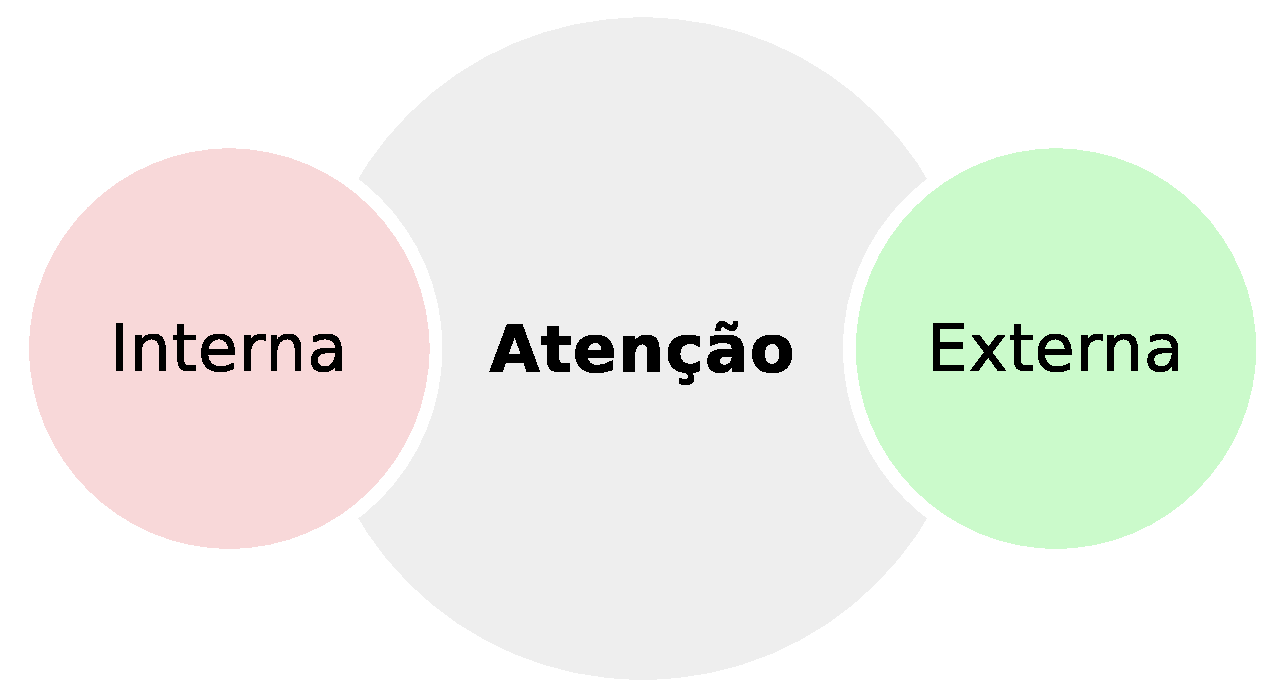
\includegraphics[width=8mm]{attention2.eps}}; }
}

%----------------------------------------------------------------------------------------
% ATTENTION MESSAGE BOX
%----------------------------------------------------------------------------------------
\newtcolorbox{remarcar}
{
  breakable,
  enhanced,
  arc      =1mm,
  colback  =colorsystemdefault!5,
  colframe =colorsystemdefault,
  leftrule =12mm,%
  overlay  ={\node[anchor=north west,outer sep=2pt] at (frame.north west) {\includegraphics[width=8mm]{remarcar.eps}}; }
}


%----------------------------------------------------------------------------------------
% CITANDO MESSAGE BOX
%----------------------------------------------------------------------------------------
% \begin{citando}
%   texto
% \end{citando}
\newtcolorbox{citando}
{
  breakable,
  enhanced,
  colback  = colorlowgray,
  colframe = colorlowgray,
  arc      = 3mm,
  left skip= 0.10 \linewidth,
  width    = 0.90 \linewidth
}

%----------------------------------------------------------------------------------------
% CATALOGRAFICA MESSAGE BOX
%----------------------------------------------------------------------------------------
% \begin{catalografica}
%   texto
% \end{catalografica}
\newtcolorbox{catalografica}
{
  breakable,
  enhanced,
  colback  = colorlowgray,
  colframe = colorlowgray
}


%----------------------------------------------------------------------------------------
% PATROCINIO MESSAGE BOX
%----------------------------------------------------------------------------------------
% \begin{patrocinio}
%   texto
% \end{patrocinio}
\newtcolorbox{patrocinio}
{
  breakable,
  enhanced,
  colback  = colorlowred,
  colframe = colorlowred
}
 % las macros compuestas usadas para la escrita


%-----------------------------------------------------------------------------------------

\hyphenation{sam-ba}


%----------------------------------------------------------------------------------------
% Para a criação do Glossário
%----------------------------------------------------------------------------------------
\makenomenclature

%%%%%%%%%%%%%%%%%%%%%%%%%%%%%%%%%%%%%%%%%%%%%%%%%%%%%%%%%%%%%%%%%%%%%%%%%%%%%%%%%%
%%%%%%%%%%%%%%%%%%%%%%%%%%%%%%%%%%%%%%%%%%%%%%%%%%%%%%%%%%%%%%%%%%%%%%%%%%%%%%%%%%
%%%%%%%%%%%%%%%%%%%%%%%%%%%%%%%%%%%%%%%%%%%%%%%%%%%%%%%%%%%%%%%%%%%%%%%%%%%%%%%%%%
%%%%%%%%%%%%%%%%%%%%%%%%%%%%%%%%%%%%%%%%%%%%%%%%%%%%%%%%%%%%%%%%%%%%%%%%%%%%%%%%%%

\begin{document}

%----------------------------------------------------------------------------------------
%	TITLE PAGE
%----------------------------------------------------------------------------------------
%%
%% ********** P�gina de Rosto
%%

%% n�o numerar a p�gina
\thispagestyle{empty}

\begin{center}

 

\colorbox{mylowgray}{
	\parbox[t]{1.0\linewidth}{
		\centering \fontsize{32pt}{80pt}\selectfont % The first argument for fontsize is the font size of the text and the second is the line spacing - you may need to play with these for your particular title
		\vspace*{0.7cm} % Space between the start of the title and the top of the grey box
		
		\hfill T�tulo Tutorial  \\
		\hfill del proyecto NOMBRE\par
		
		\vspace*{0.7cm} % Space between the end of the title and the bottom of the grey box
	}
}

%\vspace{0.9in}
%{\Large \textbf{T�tulo Tutorial de uso del programa/biblioteca}} \\ \vspace{2ex}
%{\Large \textbf{del proyecto NOMBREPROYECTO}} \\

\vspace{2in}
\begin{flushright}
\parbox{3.50in}{
Tutorial del programa/biblioteca para el uso de la 
apliaci�n/bilioteca de ...}
\end{flushright}

\vspace{0.2in}
\begin{flushright}
\parbox{3.50in}{Autor: Fernando Pujaico Rivera \\ 
Autor: AAA BBB CCC}
\end{flushright}


\vspace{1.2in}
Lima, Per� \\
2011
\end{center}





%----------------------------------------------------------------------------------------
%	COPYRIGHT PAGE
%----------------------------------------------------------------------------------------
%\cleardoublepage

\newpage
\thispagestyle{empty}

\noindent Copyright \copyright\ 2020 \myauthor\\ % Copyright notice
\noindent Esta obra é liberada com uma Licença Creative Commons 
Atribuição-NãoComercial-CompartilhaIgual 4.0 Internacional. 
Não é possível usar este arquivo excepto em conformidade com a Licença. 
Pode obter uma copia da Licença em
\url{http://creativecommons.org/licenses/by-nc-sa/4.0/}.\\ % License information

\noindent \textsc{Impresso no Brasil -- ISBN:\imprimirisbn}\\ % Publisher


\textbf{Para investir em pesquisa e colaborar com o projeto:}
\begin{tcolorbox}[breakable,colback=colorlowred,colframe=colorlowred]%%
	\sffamily
	\vspace*{\fill}					% Posição vertical
	\begin{center}					% Minipage Centralizado
	\fbox{\begin{minipage}[c][]{13.5cm}		% Largura

	\small
    Para colaborar com esta pesquisa, você pode comprar uma versão impressa do livro
    desde o seguinte endereço eletrônico:\\
    \ImprimirLinkCompraLivroImpresso ~\\
    Ou pode comprar uma versão digital desde:\\
    \ImprimirLinkCompraLivroDigital ~\\


    \hspace{0.5cm}
    Também pode colaborar com dinheiro em efetivo, desde 20 reais (5 USD), 
    pelos seguintes métodos:
    \begin{itemize}
    \item Método 1
    \item Método 2
    \end{itemize}


    \hspace{0.5cm}
    Se já colaborou com a pesquisa, e se assim o deseja, 
    sintase livre de me mandar um e-mail a \ImprimirEmail, 
    pedindo abordar um novo assunto ou aprofundar em outro.
    Sim seu pedido está dentro das minhas capacidades 
    este será agregado sem falta na seguinte edição do livro.
	\begin{flushright}
    \myauthor ~\\ 
    \end{flushright}

	\end{minipage}}
	\end{center}
\end{tcolorbox}%%



\textbf{Ficha catalográfica}
\begin{tcolorbox}[breakable,colback=colorlowgray,colframe=colorlowgray]%%
	\sffamily
	\vspace*{\fill}					% Posição vertical
	\begin{center}					% Minipage Centralizado
	\fbox{\begin{minipage}[c][5cm]{13.5cm}		% Largura
	\small
	\myauthor.
	%Sobrenome, Nome do autor
	
	\hspace{0.5cm} \mytitle: \mysubtitle   / \myauthor. --
	\imprimirlocal, \imprimiryear.
	
	\hspace{0.5cm} \pageref{LastPage} p. : il. (algumas color.) ; \imprimirsize.\\
	
	%\hspace{0.5cm} \imprimirorientadorRotulo~\imprimirorientador\\
	
	\hspace{0.5cm}
	\parbox[t]{\textwidth}{\imprimirtipotrabalho~--~\imprimireditora,~\imprimirdata.}\\

	\hspace{0.5cm}
	\parbox[t]{\textwidth}{ISBN:\imprimirisbn}\\


	
	\hspace{0.5cm}
		1. Samba de gafieira.
		2. Samba.
		3. Gafieira.
		4. Partitura de movimento.
        5. Musicalidade.
		I. Título 			
	\end{minipage}}
	\end{center}
\end{tcolorbox}%%

~\\

\noindent \textsc{Descarga gratuita da versão eletrônica em \ImprimirLinkDescargaLivro}\\

\noindent \textsc{Publicado por \imprimireditora}\\ % Publisher
\noindent \textit{Primeira impressão , \imprimirdata} % Printing/edition date


%----------------------------------------------------------------------------------------
%	DEDICATORIA
%----------------------------------------------------------------------------------------
\include{preliminares/dedicatoria} 

%----------------------------------------------------------------------------------------
%	Acknowledgements
%----------------------------------------------------------------------------------------
\cleardoublepage

\begin{center}
\Huge{\textbf{Agradecimentos}}
\end{center}

\null
\vfill
\thispagestyle{empty}

{\normalsize \it \hfill Dou muitas graças a Deus \vspace*{4pt}}


~\\

{\normalsize \it Dou muitas graças a Estevam Lawrence por me 
ajudar a resolver muitas duvidas sobre definições e uso de termos na teoria músical.
\vspace*{4pt}}


{\normalsize \it Dou muitas graças ao Prof. José Henrique de Souza (Henrique Carioca)
por suas aulas de samba no pê, 
e ter-me ensinado dinâmicas para o desenvolvimento da consciência corporal.
\vspace*{4pt}}

\begin{comment}
{\normalsize \it Dou muitas graças a \textcolor{red}{XXXXXXXXXXX} pela 
suas sugestões e revisão  do capitulo \textcolor{red}{XXXXXXXXXXX}.
\vspace*{4pt}}
\end{comment}


 

%----------------------------------------------------------------------------------------
%	PATROCINIO PAGE
%----------------------------------------------------------------------------------------
\input{preliminares/patrocinio}


%----------------------------------------------------------------------------------------
%	TABLE OF CONTENTS
%----------------------------------------------------------------------------------------
\chapterimage{chapter_head_1.pdf} % Table of contents heading image
\pagestyle{empty} % No headers
\tableofcontents % Print the table of contents itself
\cleardoublepage % Forces the first chapter to start on an odd page so it's on the right
\pagestyle{fancy} % Print headers again

%----------------------------------------------------------------------------------------
%----------------------------------------------------------------------------------------
%----------------------------------------------------------------------------------------
%	PART
%----------------------------------------------------------------------------------------
\part{Introdução}
%%%%%%%%%%%%%%%%%%%%%%%%%%%%%%%%%%%%%%%%%%%%%%%%%%%%%%%%%%%%%%%%%%%%%%%%%%%%%%%%
%% SECTION
%%%%%%%%%%%%%%%%%%%%%%%%%%%%%%%%%%%%%%%%%%%%%%%%%%%%%%%%%%%%%%%%%%%%%%%%%%%%%%%%
\section{\textcolor{green}{Historia do samba}}\index{Historia do samba}
O samba como principal manifestação da cultura brasileira está bem reconhecida no Brasil do seculo XXI;
porem, o caminho da palavra samba, ou da ideia do samba, inicia muito tempo atrás;
pois como mostraremos mais adiante, existiu uma transição entre os termos ``batuque'' e ``samba''.
Nos inícios do seculo XIX
se designava com a palavra ``batuque''  a qualquer reunião de ``pretos'' (em expressões próprias da época) realizando danças entendidas como africanas\footnote{
Porem no Brasil existem registros desta palavra desde o século XVIII \cite[pp. 85]{sandroni2001feitico}. }
\cite[pp. 54]{de4danccas} \cite[pp. 73]{lara2007memoria}.
Um exemplo disto pode ser visto numa carta ao redator do ``Correio Braziliense''  (Londres, ING),
sobre os negócios públicos em Pernambuco,
escrita o dia 3 de dezembro do 1816, e publicada em 1817 \cite[pp. 468]{batuqueBraziliense},
onde se menciona\footnote{\label{footort}A forma da escrita corresponde ao texto original}:
\begin{citando}%%
Quasi dous annos depois, o Ouvidor das Alagoas, que não tinha tido parte neste Drama,
sonhou com outro levante de pretos na sua comarca, 
fundamentado unicamente em um \textbf{batuque} de dança, 
que alguns faziam nas inmmediaçoens de um Engenho de assucar, ...
\end{citando} 
Pelo que se observa, 
a palavra ``batuque'' não se usava para referenciar a uma dança em particular e sim aos festejos dos negros em geral \cite[pp. 85]{sandroni2001feitico}.

\PRLsep{*}

Paralelamente na historia, a palavra samba estava iniciando a ser usada como parte
das expressões nestos festejos populares. 
Isto pode ser visto na ordem do dia do Quartel do Governo das Armas em
Pernambuco, 8 de julho de 1830, publicado no jornal ``Diario de Pernambuco''(PE), 
onde se  relata\footref{footort} \cite[pp. 3]{sambadiariodepernanbuco}:
\begin{citando}%%
Naõ existindo fora da Capital nos diferentes pontos,
onde se achão destacadas as Companhias deste Corpo, 
hum serviço ativo, a que sejão ellas forçadas, 
necessariamente a occiozidade dispora' 
aos mais bem conduzidos a se entreterem nas pescarias de curraes e trapaçoens de coqueiros,
em cujos passatempos sera' recebida com agrado a viola, e o \textbf{samba};
e aos peraltas, cada vez os fara' mais dezenvolvidos na conjugação do verbo surripio.
\end{citando}
Anos posteriores podemos encontrar uma dualidade no uso da palavra samba, 
tanto no sentido de música como de dança; por exemplo, no jornal ``O Capuceiro''(PE),
do dia 3 de fevereiro de 1838, temos uma referencia ao samba como música,
onde ademais se ressalta a beleza da interpretação musical;
o seguinte é um fragmento desse texto\footnote{\label{footort2}A forma da escrita corresponde ao texto original} \cite[pp. 1]{sambaperiodicoocapuceiro}:
\begin{citando}%%
Segue se, que tão perfeita na Cantoria era Catalini, ou a Pasta,
como pai Antonio descantando no seu birimbau; que tanto val huma garatuja da China,
que vinhão nos bules, e bandejas,
como as pinturas de Rafael, de Rubens, ou do Corregio;
que tão agradavel he hum \textbf{samba} d'almocreves, como a Semiramis,
a Gaza-ladra, o Tencredi, \&c. de Rossini, ...
\end{citando}
Também podemos achar outra referencia do samba no sentido musical, no jornal ``Diário do Rio de Janeiro''(RJ),
do dia 19 de abril de 1939, onde se menciona\footref{footort2} \cite[pp. 1]{sambadiariorj1}:
\begin{citando}%%
Em quanto o cortezão, o palaciano, o gamenho, o literato, o magistrado etc., 
espancão melanconias, desvanecem cuidados tomando em ricas bocetas o cheiroso rapé;
o laborioso maluto, a quem furtárão o cavalinho (que é a menina dos seos olhos)
depois de affligir-se, e praguejar em balde arranca do quijeje (bolso na celoura)
o encebado cornimboque, saca lhe com estalo e tapadoura, e chafurdando as ventas em duas,
ou trez pitadas mestras da sua torradinha, esquece-se do cavallo, resigna-se com sua sorte,
e com uma viola nas unhas zangarrêa o \textbf{samba} por uma noite inteira.
\end{citando}
Por outro lado, temos uma referencia ao samba relacionando-o com a dança, no jornal ``O Capuceiro''(PE),
do dia 12 de novembro de 1842\footnote{Só 6 anos apos referenciar o samba como música, 
no mesmo jornal, é usado o mesmo termo agora relacionado com a dança.}, 
onde mencionam\footref{footort2} \cite[pp. 5]{sambaperiodicoocapuceiro2}:
\begin{citando}%%
Aqui pelo nosso mato,\\
Qn'stava então mui tatamba,\\
Não se sabia outra cousa,\\
Senão a \textbf{dansa do samba}.
\end{citando}
Neste ultimo texto vemos que ainda se diz a \textbf{dança do samba} e não dançar o samba,
mas é possível observar como o termo vai se fusionando com a dança.
Seguindo esta linha de pensamento, 
podemos ver outro exemplo no Jornal ``O Guaycuru''(BA), do dia 26 de maio de 1846,
onde podemos ler o seguinte texto\footref{footort2} \cite[pp. 2]{sambaperiodicooguaycuru}:
\begin{citando}%%
Todavia o famigerado Salles, sem respeito algum aos institutos de sua ordem, 
foi-se pòr na Cachoeira a divertir talvez \textbf{dançando o samba}...
Que bello exemplar da vida religiosa!?
\end{citando}
Como tem sido visto, 
para esta data já se podia ver como as pessoas entendiam o samba como uma dança.
Porem, não terá que se esperar muito pra achar referencias mostrando ao samba
como uma expressão cultural em si mesma, 
uma declaração deste tipo pode ser achada no jornal ``O Cosmorama na Bahia'' (BA), 
no dia 15 de dezembro de 1849, onde menciona\footref{footort2} \cite[pp. 2]{sambaperiodicoocosmorama}:
\begin{citando}%%
Cousa já muito antiga para engordar os patinhos. 
Para o espectaculo seguinte haverá um \textbf{SAMBA} á moda da Bahia, 
em que entram os negreiros todos.
\end{citando}

\PRLsep{*}
Retomando o tema do batuque

\PRLsep{*}


Assim, como mostrado anteriormente e resumindo as ideias, 
na literatura do Brasil já temos referencias da palavra ``samba'' desde o ano de 1830; 
porem como menciona Sandroni C. no seu livro ``Feitiço decente: transformações do samba no Rio de Janeiro'', 
falando especificamente do Rio de Janeiro, 
a palavra samba foi pouco conhecida ate o último quartel do século XIX \cite[pp. 86]{sandroni2001feitico};
este dado cobrará importância quando o termo seja relacionado com as gafieiras.
Por outro lado, a palavra  ``batuque'' usada para designar festejos populares com danças, foi muito recorrente ate inícios do seculo XX, 
onde a palavra ``samba'' virou mais popular para descrever estas atividades \cite[pp. 85]{sandroni2001feitico} \cite[pp. 47]{diniz2008almanaque}; 
a Figura \ref{fig:sambacrono} descreve o uso destas palavras ao longo do tempo.
\begin{figure}[h]
  \centering
    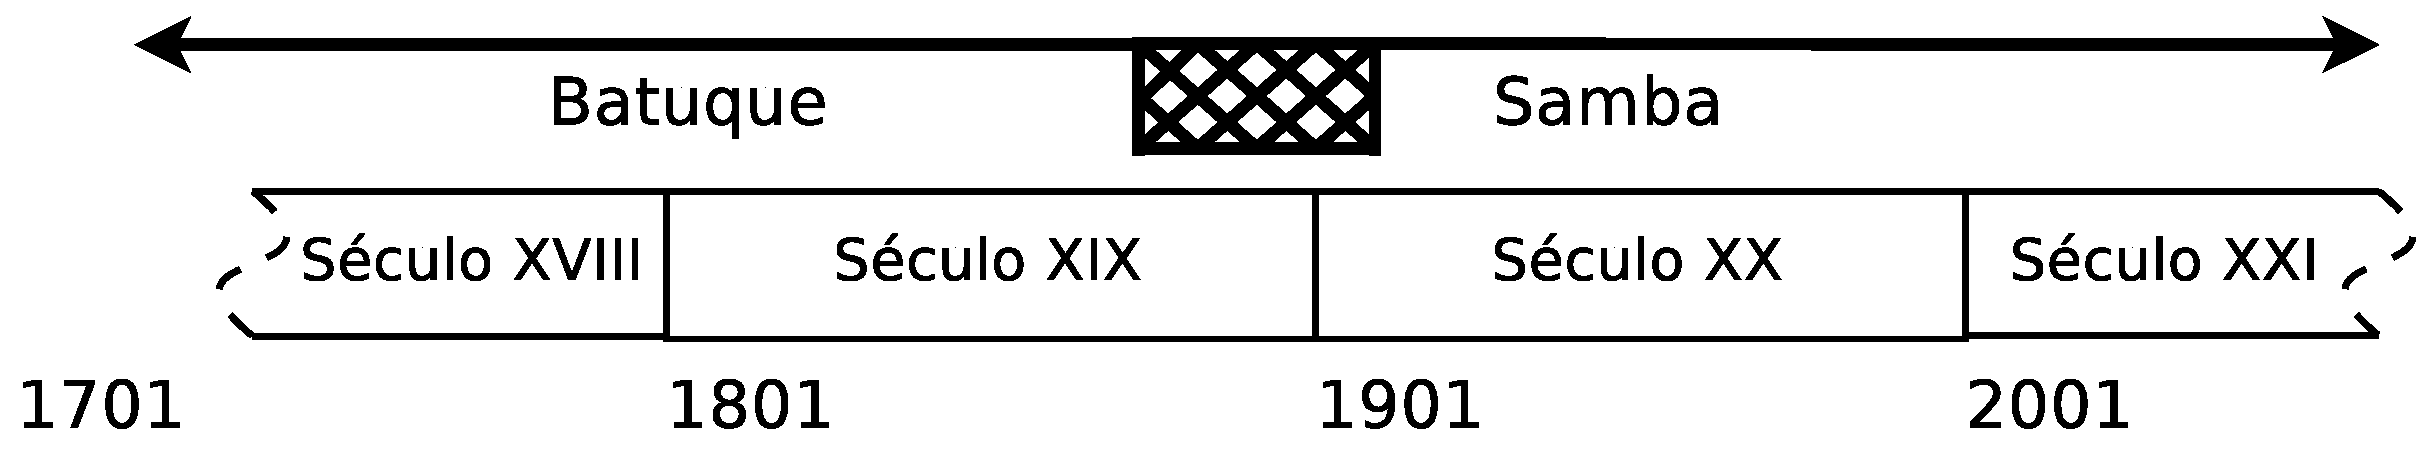
\includegraphics[width=0.85\textwidth]{chapters/cap-historia/samba-crono.eps}
  \caption{Cronologia da designação geral dos festejos de pessoas, de raça negra, no Brasil.}
  \label{fig:sambacrono}
\end{figure}


Entre as explicações da origem da palavra ``samba'', 
a mais conhecida, é a que promove que esta vem do idioma quimbundo, 
sendo derivado da palavra ``semba''  que significa umbigada \cite[pp. 47]{diniz2008almanaque} \cite[pp. 50]{da2015historia}.
Uma referencia muito conhecida deste vinculo é a descrita no livro ``O negro e o garimpo em Minas Gerais''
de Mata Machado Filho, onde ele comenta que ``os negros corrigem para semba se 
alguém lhes fala em samba'' \cite[pp. 85]{sandroni2001feitico}. Assim se vê que existe
desde antanho uma relação entre as palavras, 
samba, semba e umbigada.

\begin{comment}
Entre as danças "profanas" \cite[pp. 85]{sandroni2001feitico} afro-brasileiras o gesto da umbigada é um elemento muito caraterístico,
de modo que em 1961 Edson Carneiro definiu e englobou as danças que realizam este 
gesto como ``samba-de-umbigada'' . Assim tradições 
musicais como o samba de roda, o jongo, o lundu, o coco, o calango e o cateretê, 
seguindo Edson são englobadas com  ``samba-de-umbigada'' \cite[pp. 85]{sandroni2001feitico}.
\end{comment}


%%%%%%%%%%%%%%%%%%%%%%%%%%%%%%%%%%%%%%%%%%%%%%%%%%%%%%%%%%%%%%%%%%%%%%%%%%%%%%%%
%% Capitulo
%%%%%%%%%%%%%%%%%%%%%%%%%%%%%%%%%%%%%%%%%%%%%%%%%%%%%%%%%%%%%%%%%%%%%%%%%%%%%%%%
\chapterimage{chapter_head_2.pdf} % Chapter heading image

\chapter{Historia das gafieiras}
\index{Historia das gafieiras}

%%%%%%%%%%%%%%%%%%%%%%%%%%%%%%%%%%%%%%%%%%%%%%%%%%%%%%%%%%%%%%%%%%%%%%%%%%%%%%%%
\section{Gafieira}
\label{def:Gafieira}
\index{Gafieira}
Atualmente o termo gafieira indica um baile de clube particular, com entrada paga e frequência livre. 

\begin{itemize}
\item \textbf{1979 em adiante:} Se entende que as gafieiras são locais de lazer 
e dança onde existe bom comportamento e muita compostura,
em perfeita integração racial; de modo que, 
a gafieira é sinônimo de baile em salão espaçoso como boa música orquestral \cite[pp. 10-11]{respeitojournalbrasil1}.

\item \textbf{1932 ate antes de 1979:} O termo gafieira foi associado a lugares de baixa ralé, onde 
se aconteciam frequentemente delitos e trágicos acontecimentos \cite[pp. 11]{gafieirajournalbrasil1} \cite[pp. 12]{gafieirajournaloradical1} \cite[pp. 10-11]{respeitojournalbrasil1}.

\item \textbf{1932:} popularização do termo gafieira, apos o
incidente entre o jornalista Romeu Arêde (Picareta) e o empresario e fiscal de salão Júlio Simões,
que provocou que  Picareta publica-se uma matéria apontando 
ao clube de Júlio como uma gafieira \cite[pp. 3 - cad. 3]{juliosimoes} 
\cite[pp. 21]{efege1974maxixe} \cite[pp. 78]{coutinho2006cronistas};
pelo que este último decidiu apelidar seu exitoso ``Elite clube'' como gafieira;
espalhando-se rapidamente esta denominação a outros clubes similares. 
Assim, o termo queda vinculado a clubes de dança da classe média,
onde eram aceitos todas as pessoas sem nenhum tipo de preconceito racial, 
prévio pago da entrada \cite[pp. 6 - cad. B]{entrevistajuliojournalbrasil1}.


\item \textbf{1917 ate 1932:} 
Inícios do uso do termo gafieira, indicando bailes populares \cite[pp. 29]{instituto1987revista} de entrada paga
ou bailes criados por motivo do carnaval; sendo que, as referencias bibliográficas
achadas são nas semanas próximas ao carnaval \cite[pp. 4]{oldgafieira1} 
\cite[pp. 7]{oldgafieira2} \cite[pp. 4]{oldgafieira3} \cite[pp. 5]{oldgafieira4},
o que mostra a notoriedade que adquiriam esses eventos, ou locais, nessas datas.
\end{itemize}

%%%%%%%%%%%%%%%%%%%%%%%%%%%%%%%%%%%%%%%%%%%%%%%%%%%%%%%%%%%%%%%%%%%%%%%%%%%%%%%%
\section{Cronologia das gafieiras}


%%%%%%%%%%%%%%%%%%%%%%%%%%%%%%%%%%%%
%\PRLsep{Bailes na década de 1800}

Seguindo o jornalista Agostinho Seixas,
entre os anos de 1847 e 1848, na Cidade Velha, no Rio de Janeiro,
já existiam  bailes e clubes recreativos, 
que hoje denominaríamos como \textbf{gafieiras} \cite[pp. 11]{respeitojournalbrasil1}.
Seixas achou como primeira referencia na suas pesquisas, que entre essas datas,
Dona Francisca Pacheco da Silva, fazia um requerimento 
à ``Excelentíssima Câmara'' (que foi concedido) para a autorização 
da sua sala de bailes, na Rua da Alfândega, 327 \cite[pp. 11]{respeitojournalbrasil1} \cite[pp. 71]{perna2002samba};
este requerimento foi catalogado como sala de danças, 
com a característica de ter entrada paga.
Seguindo o fiscal que acompanhava o requerimento,
ele não achava artigo que regulamentasse esse tipo de local 
de diversão ou dança; lembremos que nessa época
o padrão era ter clubes fechados que tinham um determinado número de sócios \cite[pp. 11,12]{respeitojournalbrasil1}.



%%%%%%%%%%%%%%%%%%%%%%%%%%%%%%%%%%%%
\PRLsep{Bailes na década de 1900}


Para inícios do século XX, podiam ser achadas varias associações para negros e mestiços, 
com distintas  finalidades, como: sociedades beneficentes, literárias, dramáticas, esportivas 
e as ``sociedades dançantes e recreativas'' abertas a um público geral
\cite[pp. 154-155]{neres1999negro} \cite[pp. 71]{de2008bexiga}.
Estas associações geralmente não tinham local próprio, 
e tinham que alugar espaços que terminavam sendo salões de velhos sobrados
ou similares \cite[pp. 154-155]{neres1999negro} \cite[pp. 49]{diniz2003almanaque}.
Entre as organizações sociais recreativas mais comuns da época tínhamos, 
os cordões\footnote{Os cordões eram grupos festivos de dança e música, 
com pessoas mascaradas com figurinos de reis, de
bichos, de pajens, de guarda, etc., tocando instrumentos africanos \cite[pp. 23-24]{fernandes2001escolas}},
os ranchos\footnote{Quando os cordões desapareceram estes se transformam em ranchos (depois de 1908), 
agregaram instrumentos de corda e metais, e inciou a ser tocado a marcha-rancho,
os ranchos eram cordoes mais civilizados \cite[pp. 24]{fernandes2001escolas}} 
e os zé-pereiras\footnote{ Uma sociedade recreativa do ``Ze-pereira''
é uma sociedade dedicada a dança carnavalesca \cite[pp. 10]{simoesjournalbrasil1}} 
\cite[pp. 10]{simoesjournalbrasil1}.


Uma destas sociedades de dança do inícios do seculo XX, que agora definiríamos como gafieira, 
foi a ``Sociedade de Danças Clovis Invencivel''\footnote{Em algumas versões 
``Clovis Invencivel'' é referenciado como ``Clowns Invencíveis'' \cite[pp. 3 - cad. 3]{juliosimoes} ou 
``Clovis Invencíveis'' \cite[pp. 10]{simoesjournalbrasil1}}, 
esta foi fundada no Rio de Janeiro em 1906, 
na qual eram populares concursos de valsa, polca ou quadrilha \cite[pp. 6 - cad. B]{entrevistajuliojournalbrasil1}.
O dono da ideia da criação destes concursos foi um muito jovem e fiscal do salão, Júlio Simões,
que a seus 16 anos pensou numa sociedade de dança diferente dos da época,
que se dedicavam a ``bater bumbo'' (bailes carnavalescos ou de zé-pereira), 
a uma dedicada a ``arrasta-pés'' (bailes de salão) 
\cite[pp. 6 - cad. B]{entrevistajuliojournalbrasil1} \cite[pp. 3 - cad. 3]{juliosimoes} \cite[pp. 10]{simoesjournalbrasil1}.

Com o surgir dos lugares de baile, em 1915 \cite[pp. 1 - cad. B]{gafieira2000reis},  
Júlio Simões, foi chamado pelos sócios\footnote{Os 
sócios fundadores da ``Kanaga do Japão'' são José Constantino da Silva 
e José de Paiva Brito \cite[pp. 1 - cad. B]{gafieira2000reis}} da ``Kanaga do Japão'' para dirigir seu novo clube,
lugar de grande tradição no Rio de Janeiro, e muito popular na época,
no qual o conjunto encarregado de animar o local era chefado por Sinhô e Bulhões de Carvalho,
que receberam o título popular de ``reis da valsa'',
com torneios de dança que duravam ate 55 
minutos dançando uma valsa rápida \cite[pp. 3 - cad. 3]{juliosimoes} \cite[pp. 1 - cad. B]{gafieira2000reis} \cite[pp. 6 - cad. B]{entrevistajuliojournalbrasil1}.
Nas festas comandadas por Júlio, era comum ver dançar samba, polca, 
valsa e quadrilha, que ele mesmo marcava no salão \cite[pp. 1 - cad. B]{gafieira2000reis}. 


Para o ano 1930, estas sociedades dançantes tinham ganhado muita popularidade. 
Assim, apos a morte de um socio e o fechamento da ``Kananga do Japão'' 
em 1929 \cite[pp. 3 - cad. 3]{juliosimoes}  \cite[pp. 11]{eliteinaugura} \cite[pp. 1 - cad. B]{gafieira2000reis}, 
Júlio Simões procura a Heitor Persegani e  Hilário Jovino, 
e decidem fundar o local de danças chamado ``Elite club'' \cite[pp. 11]{eliteinaugura} \cite[pp. 13]{respeitojournalbrasil1},
agora chamado ``Elite clube'' \cite[pp. 3 - cad. 3]{juliosimoes},
na Rua Frei Caneca n. 4 - Centro, Rio de Janeiro - RJ;
sendo o 17 de julho de 1930 seu baile inaugural 
\cite[pp. 11]{eliteinaugura} \cite[pp. 3 - cad. 3]{juliosimoes} \cite[pp. 10]{simoesjournalbrasil1}.

Uma descrição de uma destas sociedades dançantes, anterior a 1931, pode ser vista no livro "O cabrocha"; 
escrita  por Jota Efegê em 1931; 
sobre a ``Sociedade Recreativa Familiar Bohemios de Botafogo'' \cite[pp. 24-26]{jotaefege},
a continuação é mostrado um extracto desse texto:
\begin{citando}%%
O salão, comquanto não fosse de grandes dimensões, era
de um tamanho regular, confinando com uma pequena saleta
onde tambem se dansava; estava bem affluido. Numa
heterogeneidade foliã, via-se desde a crioulinha blasée, sem
elegancia, desalinhada, á mulatinha pernostica de faces
avermelhadas por um carmin berrante, cabello engommado e
subjugado por travessas e grampos, num á la garçonne
forçado, mas exigido pela moda. Em meio dessas "cabrochas"
e "roxinhas", viam-se algumas moças brancas de apparencia
sobria. São as meninas que não podem fazer um vestido de
seda ou calçar sapatos de setim, para se apresentarem no
Fluminense ou no Flamengo e que nestes clubes se divertem,
ficando em evidencia por serem brancas.  %~\\
(Jota Efegê)
\end{citando}

%%%%%%%%%%%%%%%%%%%%%%%%%%%%%%%%%%%%
\PRLsep{Inícios do uso do termo gafieira}

Fazendo uma pesquisa na ``Biblioteca Digital da Fundação Biblioteca Nacional''
podemos achar referencias ao termo \textbf{gafieira} desde 1917\footnote{Mesmo 
ano em que foi lançado o samba ``Pelo telefone'', sendo um exito total no carnaval desse ano.}.


A primeira referencia pode ser vista no jornal ``O Imparcial'' (RJ),
do dia 17 de janeiro de 1917, como o título ``Batalha de confetti'',
no qual se anuncia que na rua Guimarães se terá uma grandiosa batalha,
organizada pelo ``bloco dos pesados'', conformado por \cite[pp. 4]{oldgafieira1} \cite[pp. 629]{spielmann2016reflexoes}:
\begin{citando}
Lourenço dos Santos (Lord Sorvete),\\
Antonio dos Santos (Lord Massa),\\
Antonio Lima (Lord Repinica),\\
Raul Dantas (Lord Ronqueira),\\
Almeidinha (Lord Prrrrr...!),\\
Arlindo dos Santos (\textbf{Lord Gafieira}),\\
Joaquim Mello (Lord Frango d'Agua),\\
Juvenal Branco (Lord Pé Pequeno),\\
Eudoxio dos Santos (Lord Garganta) e\\
Jorge Vença (Lord Come Bola).
\end{citando}
Pelo contexto do anuncio, e pela semelhança com os outros apelidos, 
pode-se perceber que o termo \textbf{gafieira} tem um significado alegre,
cotidiano ou extravagante, mas é difícil extrair alguma outra conclusão.

A seguinte referencia aparece um ano depois, no mesmo jornal,
no dia 8 de fevereiro de 1918, como o título ``Grande batalha de confetti'',
na qual se anuncia que a batalha é organizada pelo ``bloco da rapaziada'',
do ``\textbf{Club da Gafieira}'', a qual também terá a participação 
da \textbf{orquestra do ``Gafieira''} que tocará adoráveis tangos;
e se finaliza falando que  \cite[pp. 7]{oldgafieira2} \cite[pp. 629]{spielmann2016reflexoes}:
\begin{citando}
Serão distribuídos brindes áquelles que mais se têm distinguido nos bailes do valoroso ``\textbf{Gafieira}''.
\end{citando}
Nesta referencia, já podemos observar que a palavra gafieira é relativa à celebrações do carnaval, 
e a lugares ou eventos de bailes,
nos quais, por exemplo, se dançam tangos; 
pelo que a palavra \textbf{gafieira} é usada no nome da orquestra,
e no apelido de um integrante, o valoroso \textbf{Gafieira}.

Um ano depois na ``Gazeta de Noticias'' (RJ),
no dia 3 de março de 1919, com o título ``Club dos carnavalescos do Andarahy'' e subtitulo ``1ra Critica - A Gafieira'',
se anuncia que a ``Banda de clarins'' e a ``Banda de música'',
tocarão uma espirituosa ``charge'' aos bailes de clubs de mil réis por cabeça, 
na qual era  usada a seguinte letra \cite[pp. 5]{oldgafieira3} \cite[pp. 629]{spielmann2016reflexoes}:
\begin{citando}
Cinco tostão vale a varsa!\\
Grita o fiscal do salão:\\
Tirem as dama depressa,\\
Não perquem a casião!\\ ~\\
Sapeca o piston com força,\\
Requebra mais, já se vê!\\
Que depois da contradança,\\
A dama vai p'r'o bufê.\\ ~\\
Paga a entrada e não estrilla!!\\
Que isto aqui é uma deliça!\\
Se porte bem, seu varsista!\\
Cuidadinho e'n a poliça!...
\end{citando}
Nesta última referencia já podemos ver claramente o sentido do termo gafieira,
identificando a um lugar de dança, em especifico a esses lugares com entrada paga a mil réis por cabeça.
Para ter uma ideia de se este preço é pouco ou muito, podemos compará-lo com o 
preço do jornal em que foi publicado o texto, sendo este de 100 RS \cite[pp. 1]{oldgafieira3};
ou também por essas épocas, 
quando a entrada custava 2 mil réis o preço de uma cerveja  era  de 800 réis \cite[pp. 1 - cad. B]{gafieira2000reis}.
Outro dado interessante é o uso do termo ``fiscal de salão'', 
figura de autoridade que já estava presente 
nas sociedades dançantes do seculo XX, como por exemplo na 
``Sociedade de Danças Clovis Invencivel'' em 1906, pelo que queda claro
a que lugares se refere o termo gafieira.


Podemos ver outra noticia relativa as gafieiras, no dia 19 de janeiro de 1920, 
no jornal ``A Razão'' (RJ), no qual se
publica uma reportagem com o título 
``Charivari num club suburbano - Fechado pela policia'',
se referindo ao clube ``Fenianos de Cascadura'',
que seguindo o descrito, este clube era 
ponto de reunião de gente desclassificada, 
que realizava seus bailes os sábados e domingos,
cobrando na entrada $1\$100$ por cabeça.
O seguinte texto é uma porção daquela reportagem \cite[pp. 4]{oldgafieira4} \cite[pp. 629]{spielmann2016reflexoes}:
\begin{citando}
A policia local, que é a do $20^o$ districto,
já estava farta do trabalho que o club 
constantemente lhe dava e de receber reclamações 
dos moradores visinhos.\\
Deliberou então o delegado, dr. Coelho
Gomes, fechar o club, mais conhecido por 
``\textbf{Gafieira}'', na primeira occasião que `e apresentasse.\\
Ante-hontem, sabbado, á noite, o club 
deu o acostumado ``baile'' e ás 5 horas da 
madrugada houve, ali um ``charivari'' medonho,
que poz o largo de cascadura em polvorosa. 
\end{citando}
O termo charivari se usa para indicar música discordante, 
confusão, motim, tumulto, barafunda \cite[pp. 53]{almeida1996dicionario}, etc.
Assim, podemos ver como o termo gafieira, 
estava relacionado a clubes de dança com entrada paga,
e que era frequentado por pessoas de poucos recursos econômicos. 
Também é interessante ressaltar que as referencias achadas correspondem,
a datas próximas ao carnaval, o que mostra o vinculo ou o maior interesse 
destes locais nestas datas. 

Ainda podem ser achadas outras referencias ao termo \textbf{gafieira} na década de 1920,
nelas podemos destacar apelidos usados por professores de dança,
ou referencias de musicas com letras indicando que gafieiras 
são frequentadas por crioulas e/ou criadas.


%%%%%%%%%%%%%%%%%%%%%%%%%%%%%%%%%%%%
\PRLsep{Popularização do termo gafieira}

Seguindo o jornalista e cronista, Jota Efegê, %%Júlio Simões e o historiador,
o termo ``gafieira'' foi criado pelo cronista carnavalesco, 
Romeu Arêde\footnote{Em algumas versões está  referenciado como Romeu Aredo \cite[pp. 188]{raca1999}.}, 
também conhecido como ``Picareta'' \cite[pp. 29]{instituto1987revista}\cite[pp. 3 - cad. 3]{juliosimoes} 
\cite[pp. 21]{efege1974maxixe} \cite[pp. 78]{coutinho2006cronistas}, 
colunista da seção recreativa do ``Jornal do Brasil'' desde 1930 ate 1941
e anteriormente do vespertino ``Vanguarda'' (1922-1930) \cite[pp. 58-59]{efege1982figuras} 
\cite[pp. 6 - cad. B]{entrevistajuliojournalbrasil1};
porém não é indicada, por Jota Efegê, referencia nenhuma sobre a data de criação.
Efegê indica que o termo ``gafieira'', possivelmente deriva de 
``cabroeira''\footnote{Cabroeira: Malta de indivíduos chamados cabras, 
de capangas assalariados para assassinar ou para fazer o mal \cite{diciocabroeira}.} 
ou ``gaforinha'' \cite[pp. 3 - cad. 3]{juliosimoes}.
Por outro lado, Júlio Simões, socio e administrador do ``'Elite club', 
afirma\footnote{Seguindo a ``Revista do Instituto Histórico e Geográfico do Rio de Janeiro'' (1987),
Jota Efegê afirma que foi Romeu Arêde quem atrelou o termo gafieira aos clubes de dança no incidente no ``Elite clube''.} 
que o jornalista Romeu Arêde tinha a costume de entrar, 
comer, beber, dançar e não pagar \cite[pp.13 ]{respeitojournalbrasil1},
e que quando ele impediu ao boêmio jornalista e seus acompanhantes (5 ou 6) o ingresso no ``Elite'', 
porque a entender de Júlio o jornalista estava meio ``alegre'' devido a uns tragos a mais;
 Júlio indicou: ``Aqui tem ordem'' 
\cite[pp.13 ]{respeitojournalbrasil1} \cite[pp. 6]{gafieiraaredeout2} \cite[pp. 3 - Encontro]{gafieiraaredeout1},
indicando que só podiam passar com entrada franca ele mais uma dama ou um amigo;
o cronista então reagiu indicando a seus acompanhantes a se retirarem, 
exclamando \cite[pp. 29]{instituto1987revista} \cite[pp. 6 - Tribuna Bis]{gafieiraaredeout3}: 
\begin{citando}
Vamos embora! Isto aqui é uma gafieira!
\end{citando}
Outras referencias apontam que o que falou foi \cite[pp. 6]{gafieiraaredeout2} \cite[pp. 3 - Encontro]{gafieiraaredeout1}:
\begin{citando}
O que eu vou fazer nessa gafieira?
\end{citando}
Ao dia seguinte Picareta escreveria na sua coluna no Jornal do Brasil \cite[pp. 188]{raca1999}:
\begin{citando}
Aquele é um lugar da ralé, onde se cometem gafes em fieiras
\end{citando}
Varias referencias apontam que este incidente aconteceu em 1932 \cite[pp. 3 - Encontro]{gafieiraaredeout1} \cite[pp. 188]{raca1999}, 
porém não se menciona o dia exato. 




Assim, em qualquer das explicações da formação da palavra gafieira,
seja por ``cabroeira''+``gaforinha'' ou ``gafes''+``fieira'',
esta era uma denominação pejorativa para indicar a um local (``cabroeira'' ou ``gafes'').
É importante lembrar que o termo \textbf{gafieira}, já existia desde antes do 
incidente entre Júlio Simões e Romeu Arêde no ``Elite club'', 
especificamente se tem constância do uso desde 1917 \cite[pp. 4]{oldgafieira1},
pelo que para a data da apertura do ``Elite club'' em 1930,
este termo já estava no consciente de algumas pessoas, porém não estava popularizado;
pelo que se deduz que Romeu Arêde, por conta do incidente no ``Elite club'', 
atuou como catalisador para a popularização do termo gafieira.
%mas isto não descarta a informação de Jota Efegê que indica que foi Arêde quem criou o termo,
%pois  Efegê não menciona uma data especifica.

Júlio simões apos o incidente no ``Elite club'', 
decide devolver a piada e apelidar seu local como 
``Gafieira'', conservando o nome de clube, 
mas transformando-se na pratica em ``Gafieira Elite'' \cite[pp. 79]{moura1995tia} \cite[pp. 6 - Tribuna Bis]{gafieiraaredeout3}.
Por este incidente e suas repercussões, 
muitos autores consideram a ``Elite'' como a primeira gafieira do Brasil \cite{cabral2016elisete} \cite[pp. 84]{cabral1996escolas}.
Consequentemente, e em palavras de Jota Efegê, 
se considera a Júlio Simões como o criador das gafieiras \cite[pp. 3 - cad. 3]{juliosimoes}.

Nesse ponto da historia, 
o nome ``gafieira'' cobrou muita relevância e locais de dança apelidados como gafieiras surgiram no Rio de Janeiro;
depois de tudo, já existissem lugares com estas caraterísticas desde inícios do século XX \cite[pp. 49]{diniz2003almanaque}.
Os salões foram criadas a semelhança dos bailes de salão da classe média ou alta \cite[pp. 78]{coutinho2006cronistas}; 
porém, no caso das gafieiras, estas eram abertas ao público prévio pago da entrada.
A Figura \ref{fig:gafieiracrono} mostra a cronologia do uso da palavra gafieira para os salões de dança no Rio de Janeiro.
\begin{figure}[h]
  \centering
    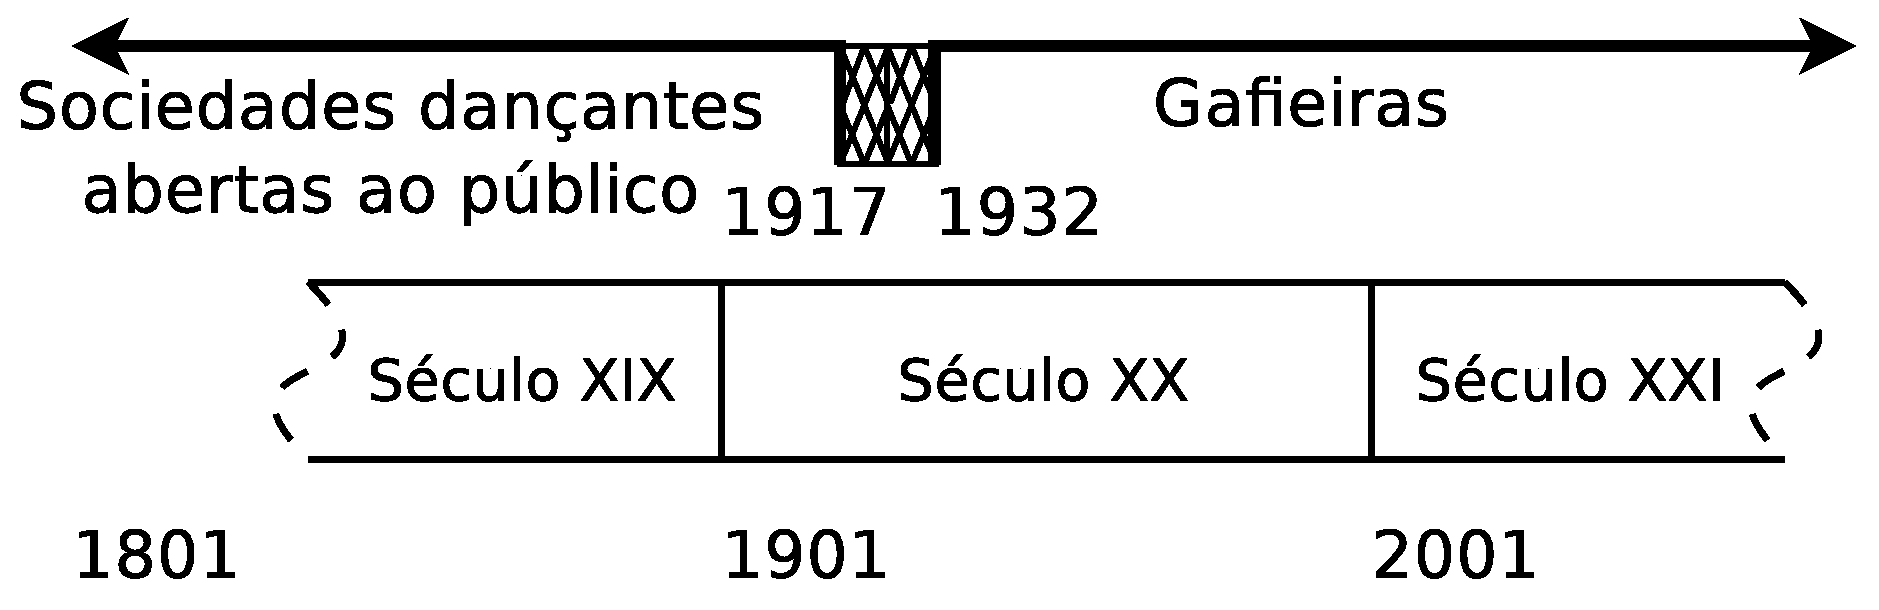
\includegraphics[width=1.0\textwidth]{chapters/cap-historia-gafieiras/gafieira-crono.eps}
  \caption{Cronologia da designação de gafieira para os salões de dança no Rio de Janeiro.}
  \label{fig:gafieiracrono}
\end{figure}

\PRLsep{Delitos vinculados com as gafieiras}

Podemos achar uma referencia ao termo gafieira no jornal ``O Radical'' (RJ),
no dia 8 de setembro de 1932 \cite[pp. 12]{gafieirajournaloradical1},
com o titular:
\begin{citando}%%
A sahida do baile: Por causa de Aracy, o estivador foi ferido á baia.\\
... Na rua Domingo Lopes, n. 243, em Madureira, está situado o club de dança Ideal, 
conhecido pelos moradores locaes por ``Gafieira''.
\end{citando} 
Ao dia seguinte, 9 de setembro de 1932, o jornal ``A Batalha'' (RJ), 
usava também a palavra ``gafieira'' para se referir ao mesmo incidente \cite[pp. 8]{gafieirajournalabatalha1}.

O ``Jornal do Brasil'', o dia 9 de janeiro de 1934, 
usa também a palavra gafieira \cite[pp. 11]{gafieirajournalbrasil1}, com o titular:
\begin{citando}%%
À porta de uma ``gafieira''.
Ainda o conflito da madrugada de domingo no largo de Madureira.
Faleceu um dos soldados no Hospital da Policia Militar. 
Ha no largo de Madureira uma sociedade dansante, mais conhecida por ``gafieira'', 
com entradas retribuidas, ondem de quando em quando, se registram conflitos, 
alguns de graves consequências...
\end{citando} 
Como é visto nas refecerias antes mostradas, e guardando semelhança com outras coincidências
posteriores que podem ser achadas na ``Biblioteca Digital da Fundação Biblioteca Nacional''; 
o termo gafieira, estava associado a lugares considerados perigosos;
isto propiciado pelo aumento do número de locais que se atribuíam este nome, junto com 
a diversidade e cultura  do seu público e administradores.
Porém, este não seria o padrão pelo qual se regiam todas as gafieiras, 
e certamente a conotação mais perigosa ou pejorativa iria mudando no tempo. 

\PRLsep{A gafieira limpa seu nome}

Por exemplo, sobre o Elite Club,  nos sabemos que funcionava as quintas, sábados e domingos,
e existia um fiscal no salão (o velho Russo)\cite[pp. 37]{gafieirajournalmanchete}, 
que fazia cumprir estritamente as normas de bom-tom, comportamento social e respeito ao ambiente, como todo clube familiar precisa ter \cite[pp. 12]{respeitojournalbrasil1}; de modo que, 
não eram admitidas damas que não estivessem de sapatos de salto alto \cite[pp. 37]{gafieirajournalmanchete};
homens embriagados não entravam e o traje indispensável era o paletó e gravata, 
ou no mínimo camisa fechada \cite[pp. 6 - cad. B]{entrevistajuliojournalbrasil1}.
O cavaleiro não podia abraçar a dama nem sentado na cadeira \cite[pp. 6 - cad. B]{entrevistajuliojournalbrasil1},
né dançar de rosto colado, ou por a mão nas costas da dama sem usar lenço \cite[pp. 10]{simoesjournalbrasil1}, 
quem fiscalizava, na porta, era um preto velho tratado por todos de ``titio''  \cite[pp. 37]{gafieirajournalmanchete}.
Se alguma regra não era cumprida, o seu Júlio, jogava a qualquer um para fora \cite[pp. 6 - cad. B]{entrevistajuliojournalbrasil1}.
Nos bailes dedicados ao padroeiro, todo 20 de janeiro, era obrigatório vestir de branco,
já seja no traje ou no vestido, incluindo sapatos e camisas \cite[pp. 37]{gafieirajournalmanchete}.
Tão grande era o censo de ordem dos frequentadores do Elite Club, 
que lhe era permitido operar estando a menos de 80 metros de um hospital,
sendo que nessa época existia a Lei n. 1.590 de 1924, 
seguindo a qual nenhuma casa de diversões podia estar a menos de 200 m de estabelecimentos hospitalares,
Ate o próprio Delegado Dulcídio Gonçalves, da Delegacia de Costumes,
dispensava-se de mandar policiar o Elite.
``À casa do Júlio não precisa de policiamento'', dizia o Delegado Dulcídio
\cite[pp. 5]{simoesjournalalutademocratica1}.


Assim, ao transcorrer dos anos, essa visão popular mais obscura da palavra gafieira foi mudando;
pelo qual o jornalista Francisco Duarte, o dia 12 de agosto de 1979,
escreve no Jornal do Brasil (RJ) sobre este assunto com o título:
``Gafieira - Tratado geral do ambiente que exige respeito'' \cite[pp. 10]{respeitojournalbrasil1}:
\begin{citando}%%
... o verbete Gafieira com o significado de baile reles, arrasta-pé, baile popular de baixa categoria.
No passado, encarada com má vontade pelos puristas do léxico e pela burguesia republicana dançante,
pode ter sido assim. Mas em 1979 -- e cabe aos dicionaristas verificar in loco --
gafieira é baile de clube particular, com entrada paga e freqüência livre, 
local de lazer e dança onde existe bom comportamento e muita compostura,
em perfeita integração racial.\\
(Francisco Duarte)
\end{citando}
Além da afirmação anterior, 
o jornalista explica como a ``Delegacia de Diversões Públicas'' classifica as casas de dança;
assim temos: 
\begin{itemize}
\item ``boates'', que são bar restaurantes com pista de dança e palco para show;
\item ``cabarés'', onde se bebe, come, dança e se tem espetáculos de variedades;
\item ``dancings'' onde se dança mediante pagamento em cartões e picotes; e 
\item ``inferninhos'' que são boates de baixa categoria, 
frequentados por pessoas de vida irregular e onde se toca música barulhenta.
\end{itemize} 
Em palavras de Duarte, ``Gafieiras são sinônimos de baile em salão espaçoso como boa música orquestral'' \cite[pp. 11]{respeitojournalbrasil1}.




%%%%%%%%%%%%%%%%%%%%%%%%%%%%%%%%%%%%%%%%%%%%%%%%%%%%%%%%%%%%%%%%%%%%%%%%%%%%%%%%
%% SUB SECTION
\section{Estatutos da gafieira}\index{Estatuto da Gafieira}
Os ``Estatutos da Gafieira'' é uma composição musical escrita, por Billy Blanco;
esta foi interpretada por primeira vez na voz de Inezita Barroso, 
numa gravação da "RCA Victor" em janeiro de 1954 \cite{musicaestatuto};
O seguinte texto mostra a letra da música numa 
versão publicada no jornal ``Cinelândia''  (RJ),
na segunda quinzena de dezembro de 1955 \cite[pp. 95]{musicaestatutojournal1955}.
\begin{citando}%%
\center{Moço! Olha o vexame!}\\
O ambiente ``ingige'' respeito!\\
Pelos estatutos da nossa gafieira\\
Dance a noite inteira, mas dance direito!\\
Aliás, pelo artigo 120,\\
O cavalheiro que fizer o seguinte:\\
Subir nas paredes, dançar de pé pro ar,\\
Morar na bebida sem querer pagar,\\
Abusar da umbigada de maneira folgazã,\\
Prejudicando hoje o bom crioulo de amanhã,\\
Será distintamente censurado!\\
Se balançar o corpo, tá na mão do delegado!\\
Balançou o corpo? tá na mão do delegado!\\
\end{citando}
O texto é uma tentativa bem-humorada do autor de descrever o que acontecia 
nas gafieiras, porém na época da escrita desta popular samba, não
existiam tais estatutos\footnote{Estatutos, no sentido de regulamento, 
ordenança o conjunto de normas legais pelas que se regula o funcionamento de uma corporação ou associação.};
existia um código de costumes sim \cite[pp. 13]{respeitojournalbrasil1} em alguns salões, 
mas cada casa de dança imponia estes no seu local a critério do fiscal do salão ou dos 
donos \cite[pp. 10]{simoesjournalbrasil1} \cite[pp. 6 - cad. B]{entrevistajuliojournalbrasil1} \cite[pp. 37]{gafieirajournalmanchete},
isto é confirmado por um depoimento realizado por 
Billy Blanco no 8 de julho de 2011 \cite[pp. 56]{depoimentobilly}; o texto a seguir
mostra um fragmento dessa entrevista.

\begin{citando}%%
"Observando os acontecimentos de uma gafieira, então, eu imaginei
coisas, porque o compositor vive muito da imaginação. E eu criava situações 
possíveis de serem acontecidas na gafieira, ou então narrava o que
acontecia realmente. Por exemplo, no [samba] Pistom de Gafieira, tinha
um cidadão que era pistonista da orquestra que sempre tocava forte para
disfarçar quando a polícia vinha chegando. Doutra feita, eu tive a ideia
de fazer o estatuto para a gafieira. Então eu humorizei, porque ninguém
dança de pé pro ar, nem sobe em parede, não é? Mas a gente cria uma
extravagância dessas para dar uma certa graça, um certo sentido à música.
Na época, não havia código nenhum, eu apenas criei aquilo e muitas gafieiras 
depois tinham esse estatuto na parede para quem quisesse cantar.
Você vê que as regras do estatuto são umas regras brincalhonas, não é?" 
~\\
(Billy Blanco)
\end{citando}

Mesmo observando que as regras propostas pelo autor tem um caráter humorístico e sarcástico,
o texto foi adotado rapidamente pelas gafieiras, como um chamado a reflexão sobre umas
normas básicas a serem tidas em conta no salão, pois tem um grau de bom senso. Por exemplo: 
A linha 7, pode ser interpretada como uma indicação a 
não fazer movimentos aéreos na pista de dança,
ou  evitar movimentos capoerísticos; tudo isto
pelo evidente espacio reduzido e compartilhado que existe na pista de dança, 
além de que os movimentos aéreos estão pensados para ser
executados em apresentações e não em danças sociais. 
A linha 8, nos lembra o respeito ao parceiro; pois a pessoa que dança precisa
estar no controle de suas faculdades físicas e mentais; 
no caso dos \hyperref[def:Condutor]{\textbf{condutores}}\footnote{\label{footlab:conducao}Nas danças sociais é comumente usado o paradigma da condução; 
no qual, no casal, uma pessoa assume o papel de \hyperref[def:Condutor]{\textbf{condutor}} dos movimentos e 
a outra pessoa assume o papel de \hyperref[def:Seguidor]{\textbf{seguidor}}, este recebe a informação da condução e retorna uma resposta corporal.}, 
para estar atentos ao salão e cuidar do seu par enquanto os movimentos são executados, 
e no caso do \hyperref[def:Seguidor]{\textbf{seguidor}}\footref{footlab:conducao} para evitar problemas
nos giros e outros movimentos que precisem  controle do eixo do corpo.
As linhas 9 e 10 indicam sobre um conjunto de expressões artísticas 
afro-brasileiras emolduradas no século XIX com o nome de ``samba umbigada'' \cite[pp. 47]{diniz2008almanaque} \cite[pp. 85]{sandroni2001feitico}; nestas danças existe
um movimento chamado ``umbigada'' \cite[pp. 50]{da2015historia} que dá nome à dança, na qual o ventre do homem e da mulher batem geralmente para indicar
a troca de dançarino; assim as linhas 9 e 10 se referem a
 evitar ``abusar'' de movimentos de umbigada que provem de danças que não eram bem vistas na época e eram consideradas gentílicas \cite[pp. 85]{sandroni2001feitico}.
Finalmente,
a linha 12 fala sobre balançar o corpo, que seguindo o contexto cultural, 
pode indicar não agir como bêbado\footnote{``Balançar o corpo; agitar, como o bebado, mal firme, e outros táes'', Diccionario da lingua portugueza, 1858 \cite[pp.296]{diccionario1858}.}, ou em outras palavras,
com pouca elegância ou respeito,
caso contrario seria levado à delegacia!.



%%%%%%%%%%%%%%%%%%%%%%%%%%%%%%%%%%%%%%%%%%%%%%%%%%%%%%%%%%%%%%%%%%%%%%%%%%%%%%%%
%% Capitulo
%%%%%%%%%%%%%%%%%%%%%%%%%%%%%%%%%%%%%%%%%%%%%%%%%%%%%%%%%%%%%%%%%%%%%%%%%%%%%%%%
\chapterimage{chapter_head_2.pdf} % Chapter heading image

\chapter{Historia da música do samba}\index{Música do samba}

O samba é uns dos gêneros musicais mais conhecidos no Brasil do século XXI;
entre estes gêneros mais populares, temos por exemplo, ao ``forró'' e ao ``Sertanejo'';
sendo que o samba se distingue entre eles, 
como a principal expressão popular da música brasileira \cite[pp. 47]{diniz2008almanaque}.\\


%\begin{definition}[Samba:]
\begin{remarcar}
\textbf{Samba:}
\index{Samba}
\label{ref:samba} 
No Brasil, a palavra samba  é usada como designação de uma dança popular  e música  em compasso binário (basicamente 2/4), 
de ritmo sincopado e andamento variado \cite[pp. 290]{dourado2004dicionario} \cite[pp. 684]{marcondes1977enciclopediav2};
ambos com uma forte influencia da cultura africana \cite[pp. 290]{dourado2004dicionario};
representando estas desde inícios do século XX, 
uma expressão cultural, urbana e popular no Brasil \cite[pp. 684]{marcondes1977enciclopediav2} \cite[pp. 290]{dourado2004dicionario}.
\end{remarcar}
%\end{definition}

A popularização, o reconhecimento comercial e a representatividade cultural no consciente coletivo do brasileiro,
não sempre estiverem alinhados com o samba, 
sendo que esta conjunção teve seu origem a inícios do seculo XX, 
com o inicio das gravações comerciais, em disco, e a consequente popularização comercial do gênero.

 As reuniões na casa da Tia Ciata foram o cenário da criação do samba-maxixe ``Pelo telefone'',
 composto, em 1916, 
por Ernesto dos Santos (Donga) e Mauro de almeida (Peru dos Pés Frios) \cite[pp. 34]{diniz2006almanaque} \cite[pp. 49]{diniz2008almanaque} \cite{musicapelotelefone} \cite[pp. 28]{diniz2003almanaque}.
\begin{remarcar}
Dados da música \textbf{Pelo telefone}:
\index{Pelo telefone}
\begin{itemize}
\item 1996, novembro 6, é presentada uma petição de registro no
Departamento de Direitos Autorais, da Biblioteca Nacional, 
do Rio de Janeiro (RJ), 
por   Ernesto dos Santos  para o samba carnavalesco \textbf{Pelo telefone} \cite[pp. 599]{marcondes1977enciclopediav2}.
\item 1996, novembro 16, Ernesto dos Santos, 
anexa à petição um atestado que afirma que 
o samba carnavalesco \textbf{Pelo telefone}, 
foi executado em público pela primeira vez no
Cine-Teatro Velho o dia 25 de outubro de 1916,
este atestado foi subscrito por M.P. Cabrita e Julio Suckow \cite[pp. 599]{marcondes1977enciclopediav2}.
\item 1996, novembro 27, o registro foi efetivado com o número 3.295 \cite[pp. 599]{marcondes1977enciclopediav2}.
\item 1996, dezembro 16, a partitura manuscrita para piano, feita por Pixinguinha, 
estava dedicada a Mauro de Almeida e Norberto Amaral (Morcego) é
publicada no Instituto de Artes Gráficas, do Rio de Janeiro \cite[pp. 599]{marcondes1977enciclopediav2}.
\item Carnaval de 1917, a música foi sucesso   \cite[pp. 599]{marcondes1977enciclopediav2}  \cite[pp. 35]{diniz2006almanaque}, 

\item 1917, É realizada a primeira gravação de  \textbf{Pelo telefone}, feita pela Banda Ondeon (121.313-B), 
onde consta como autor unicamente Donga, 
sendo esta uma gravação instrumental \cite{musicapelotelefone} \cite[pp. 599]{marcondes1977enciclopediav2},
e  fabricada especialmente para a Casa Edison, pela fabrica Ondeon, com número de patente 3465.
\item 1917, É realizada a segunda gravação, onde os versos de \textbf{Pelo telefone} seriam conhecidos pelo público;
foram encargados da interpretação, ``Bahiano\footnote{Está 
escrito Bahiano na capa do disco, porem muita referencias bibliográficas,
escrevem Baiano.} e côro'' (121.322-A), acompanhado somente de violão e cavaquinho. 
Esta gravação é fabricada especialmente para a Casa Edison, pela fabrica Ondeon, com número de patente 3465,  
e constam como autores Donga e Mauro de Almeida 
(música e letra respetivamente) \cite[pp. 599]{marcondes1977enciclopediav2} 
\cite[pp. 35]{diniz2006almanaque}  \cite{musicapelotelefone}.
\end{itemize}
\end{remarcar}

Porem, esta autoria é questionada por compositores contemporâneos de Donga, que alegam que
ele modificou e apropriou-se de uma criação coletiva e anônima, 
de tradição oral cantada por todos na casa da Tia Ciata \cite{musicapelotelefone} \cite[pp. 35]{diniz2006almanaque} \cite[pp. 49]{diniz2008almanaque};
assim, o dia 4 de Fevereiro de 1917, no ``Jornal do Brasil'' (RJ), Tia Ciata, Sinhô e outros,
protestaram a usurpação da autoria, parodiando à versão gravada, como é visto a seguir \cite[pp. 17]{TiaCiataVsDonga} \cite[pp. 118-119]{sandroni2001feitico}:
\begin{citando}%%
\begin{center}
1ra PARTE\\
Pelo telefone a minha boa gente\\
Mandou-me avisar!...\\
Que meu bom arranjo era oferecido\\
Para se cantar!...\\
~\\
2da PARTE\\
Ai! Ai! Ai!... leve a mão\\
A' consciencia!...\\
Meu bem,\\
Ai! Ai! Ai!... porque\\
Tanta presença!...\\
Meu bem!\\
~\\
1ra PARTE\\
O que cara dura de dizer nas rodas\\
Que este arranjo é teu?...\\
É do bom Hilario e da velha Ciatta\\
Que o Sinhô escreveu!...\\
~\\
3ra PARTE\\
Tomara que tu apanhes,\\
Para não tornar a fazer isso,\\
Escrever o que é dos outros,\\
Sem olhar o compromisso.
\end{center}
\end{citando}%%

Por outro lado, durante muito tempo ``Pelo telefone'' foi considerado o primeiro samba gravado;
porem, segundo Flávio Silva  já existiam outros discos anteriormente com a etiqueta samba,
inclusive pela Casa Edison, que gravou ``pelo telefone''  \cite[pp. 96]{hertzman2013making} \cite[pp. 118]{sandroni2001feitico}.

Apesar de todos estes problemas, há uma contribuição de ``Pelo telefone'' à música, 
esta foi a indicação do gênero ``samba'' no selo do disco junto ao registro na Biblioteca Nacional,
que abriu o caminho para à difusão comercial e urbanização do gênero samba,
 e seu consequente prestigio \cite{musicapelotelefone} \cite[pp. 49]{diniz2008almanaque};
como corrobora Flávio Silva, que no seu levantamento bibliográfico deteta que, no carnaval, o termo
samba aparece na prensa  de Rio de Janeiro \cite[pp. 118]{sandroni2001feitico}, 
\begin{itemize}
\item 3 vezes em 1916, 
\item 22 vezes em 1917 e
\item 37 vezes em 1918.
\end{itemize}

\section{Qual é a família do samba (música)?}
\begin{remarcar}
\index{Batucada}
\index{Música do samba!Batucada}
\textbf{Batucada (música):} É a denominação dada ao ritmo do 
\hyperref[ref:batuquedanca]{\textbf{batuque}}\footnote{Para 
mais informação sobre o batuque ir a páginas \pageref{ref:batuquedanca1800} e \pageref{ref:batuquedanca}.} 
e é também usado como sinônimo deste \cite[pp. 89]{marcondes1977enciclopedia}.
\end{remarcar}
Existem muitos subgêneros em que o samba é tocado e cantado, alguns tiveram vida efêmera,
e outros perduraram no tempo, a continuação serão listados alguns destes subgêneros.

\begin{description}

%% MARACATU


\item[Bossa nova:] 
\index{Música do samba!Bossa nova}
\index{Música do samba!Samba-bossa}
Também chamado \textbf{samba-bossa}, este gênero pode ser entendido como um samba-choro modernizado \cite[pp. 63]{reinato2010musica}.
A bossa nova surgiu  na década de 1950 \cite[pp. 130]{perna2002samba},
apos a segunda gerra mundial pela influencia da cultura norte-americana, motivada 
pela política desenvolvimentista do presidente do Brasil, Juscelino Kubitschek (1956 - 1961) \cite[pp. 15]{de2003tem}.
Esta variante do samba é caraterizada por uma sofisticada harmonia e um modo diferente de dividir o fraseado, 
agregando influencias do impressionismo erudito do jazz  \cite[pp. 130]{perna2002samba} \cite[pp. 15]{de2003tem}. 

O inicio da bossa nova, e sua popularização, 
marcou um período de dificuldade para o choro e seus instrumentistas,
pelo desinteresse  do choro ao ser considerada coisa de velho, quadrada, nacionalista, de aposentado e suburbano \cite{rizzi2016musica}.

A bossa nova foi inaugurada usando composições e interpretações de, Antônio Carlos Jobim (Tom Jobim) e Carlos Lyra,
a poesia de Vinícius de Moraes, e
a batida do violão de João Gilberto \cite[pp. 130]{perna2002samba}  \cite[pp. 15]{de2003tem}.
\begin{example} ~

\begin{itemize}
\item ``Chega de saudade'' (1958) de Vinícius de Moraes e Antônio Carlos Jobim \cite{castro2016chega} \cite{tomjobim}.
\item ``Garota de Ipanema'' (1962) de Vinícius de Moraes e Antônio Carlos Jobim \cite{tomjobim}.
\end{itemize}
\end{example}

\item[Choro:] 
\index{Música do samba!Choro}
Este é um gênero musical brasileiro, surgido na cidade de São Sebastião, Rio de Janeiro, por volta de 1870 \cite[pp. 14]{diniz2003almanaque} \cite[pp. 132]{perna2002samba} \cite[pp. 64]{reinato2010musica},
com espirito melancólico que mesclou o samba com  estilos europeus como schottisches, polcas,
valsas e outros gêneros em voga na época  \cite[pp. 64]{reinato2010musica} \cite[pp. 79]{dourado2004dicionario} \cite[pp. 132]{perna2002samba}.
O choro ou chorinho é uma composição livre, em ritmo binário, 
tradicionalmente composto em três seções com 16 compassos cada uma \cite[pp. 64]{reinato2010musica}.
Para o ano de 1910 este já era um gênero consolidado \cite[pp. 12]{diniz2003almanaque}.

Entre os instrumentos mais populares que constituíram o choro na época da criação, 
estão o violão, o cavaquinho e a flauta transversal;
na década de 1930 foram incorporados, o pandeiro, o bandolin e a clarineta \cite[pp. 64]{reinato2010musica} \cite[pp. 79]{dourado2004dicionario} \cite[pp. 132]{perna2002samba};
todos estes instrumentos dão à música um aspecto sentimental melancólico e ``choroso'', e
é de ali que alguns autores apontam que surge o nome do estilo \cite[pp. 132]{perna2002samba};
porem, seguindo Batista Siqueira, 
o termo choro vem da fusão do verbo ``chorar'' e ``chorus'', coro em latim \cite[pp. 13]{diniz2003almanaque}.

O flautista, Joaquim Callado (Joaquim Antônio da Silva Callado 1848-1880) 
é conhecido como ``O pai do choro'';
este foi o autor de 66 melodias, e conseguiu conciliar: 
uma sólida formação musical com um grande poder de improvisação  \cite[pp. 15]{diniz2003almanaque} \cite[pp. 64]{reinato2010musica}.
Entre os grandes interpretes do gênero temos a:
Pixinguinha, Waldir Azevedo, Jacó do Bandolim, Dinho Sete Cordas, Altamiro Carillo \cite[pp. 79]{dourado2004dicionario}, etc.

\begin{example} ~

\begin{itemize}
\item ``A flor amorosa'' de Joaquim Callado \cite[pp. 8]{livingston2005choro} \cite[pp. 15]{diniz2003almanaque}.
\item ``Cruzes, minha prima'' de Joaquim Callado \cite[pp. 15]{diniz2003almanaque}.
\item ``Querida por todos'' de Joaquim Callado \cite[pp. 15]{diniz2003almanaque}.
\item ``Tico-Tico no fubá'' (1917) de Zequinha de Abreu, sem letra e chamado na época ``Tico-Tico no farelo'' \cite[pp. 6]{marcondes1998enciclopedia} \cite[pp. 39,91]{diniz2003almanaque}
\item ``Carinhoso'' (1927) Pixinguinha   \cite[pp. 133]{perna2002samba}.
\item ``Brasileirinho'' (1947) de Valdir Azevedo  \cite[pp. 133]{perna2002samba}.
\item ``Noites cariocas'' Jacob do Bandolim \cite{diniz2003almanaque}.
\item ``Doce de coco'' Jacob do Bandolim \cite{diniz2003almanaque}.
\item ``Vibrações'' Jacob do Bandolim \cite{diniz2003almanaque}.
\item ``Melodia celestial'' de Raul Barros \cite[pp. 130]{livingston2005choro}.
\end{itemize}
\end{example}

\item[Marchinha:] 
\index{Música do samba!Marchinha}
\index{Música do samba!Marcha}
Também chamado \textbf{marcha} \cite[pp. 448]{marcondes1977enciclopedia},
é um gênero de música popular, em compasso binário (2/4) de andamento vivo, 
está provem dos ranchos e cordões carnavalescos, a coreografia consiste num andar ritmado e em voltas. \cite[pp. 65]{reinato2010musica}.

A diferença entre a marcha-rancho e  a marchinha está no jeito cadenciado, 
melodioso e harmônico da primeira, em contrapartida ao estilo espevitado,
jocoso, cheio de sátiras e com letras de duplo sentido da segunda \cite[pp. 84,87]{diniz2008almanaque}.

A primeira marchinha carnavalesca, titulada ``Ô abre alas'', foi escrita em 1899 por Chiquinha Gonzaga \cite[pp. 84, 239]{diniz2008almanaque}.

\begin{example} ~

\begin{itemize}
\item ``Ô abre alas'' (1899) Chiquinha Gonzaga  \cite[pp. 84, 239]{diniz2008almanaque}.
\item ``Os calças-largas'' (1927) Lamartine Babo e Francisco Gonçalves de Oliveira,
interpretado por Frederico Rocha \cite[pp. 91]{diniz2008almanaque}.
\item ``O teu cabelo não nega'' (1932) de Lamartine Babo e dos Irmãos Valença, interpretado por Castro Barbosa \cite[pp. 99]{diniz2008almanaque}.
\item ``Balancê'' (1936) de Alberto Ribeiro e Braguinha interpretado por Carmen Miranda \cite[pp. 83]{diniz2008almanaque}.
\item ``Mamãe, eu quero'' (1937) de Vicente Paiva e Jararaca \cite[pp. 584]{marcondes1977enciclopediav2} \cite[pp. 93]{diniz2008almanaque}.
\item ``Cabeleira do Zezé'' (1964) de João Roberto Kelly e Roberto Faissal interpretado por Jorge Goulart \cite[pp. 117,118]{diniz2008almanaque}.
\item ``Pierrô apaixonado'' (1936) de Heitor dos prazeres e Noel Rosa \cite[pp. 1070]{marcondes1977enciclopediav2} \cite[pp. 53]{diniz2008almanaque}.
\end{itemize}
\end{example}

\item[Marcha-rancho:] 
\index{Música do samba!Marcha-rancho}
Inicialmente chamado de \textbf{marcha de rancho} \cite[pp. 448]{marcondes1977enciclopedia}
é um gênero de musica popular, em compasso binário andante, 
está provem da musica produzida pelas chamadas orquestras dos ranchos e cordoes 
carnavalescos de fins da década de 1910 \cite[pp. 65]{reinato2010musica} \cite[pp. 448]{marcondes1977enciclopedia}.
A marcha-rancho tem um ritmo mais dolente que o das marchas (marchinhas)
e tem muito mais trabalho na parte melódica. 
Este gênero foi desenvolvido por autores reconhecidos, 
a finais da década de 1920;
onde podemos ver composições como a marcha rancho com coro ``moreninha'',
gravada no disco Ondeon n. 123.208, em 1927 \cite[pp. 448]{marcondes1977enciclopedia}.

\begin{example} ~

\begin{itemize}
\item ``Moreninha'' (1927) de Eduardo Souto \cite[pp. 448]{marcondes1977enciclopedia}
%\item ``Bem-te-vi'' (1933) de Lamartine Babo interpretado por Gastão Formenti \cite[pp. 916]{marcondes1977enciclopediav2} \cite[pp. 87]{diniz2008almanaque}.
\item ``As Pastorinhas'' (1938) de Carlos Alberto Ferreira Braga (Braguinha ou João de Barro) e Noel Rosa, 
inicialmente titulado ``Linda pequena''.
Apos modificação de nome, letra e música, 
foi regravado e interpretado por Sílvio Caldas \cite[pp. 1066]{marcondes1977enciclopediav2} \cite[pp. 87]{diniz2008almanaque}.
\item ``Marcha da quarta-feira de cinzas'' (1962) de Vinícius de Moraes e Carlos Lyra \cite[pp. 1021]{marcondes1977enciclopediav2} \cite[pp. 91]{diniz2008almanaque}.
\item ``A banda'' (1966) Chico Buarque interpretada por Nara Leão \cite[pp. 90]{diniz2008almanaque}.
\item ``Máscara negra'' (1967) José Flores de Jesus (Zè Kéti)  \cite[pp. 89]{diniz2008almanaque}.
\item ``Flor do sereno'' (2000)  \cite[pp. 88]{diniz2008almanaque}.

\end{itemize}
\end{example}

\item[Maxixe:] 
\index{Música do samba!Maxixe}
Também chamado \textbf{machiche}\footnote{Seguindo Batista Siqueira, 
o termo maxixe é uma corruptela de ``Macho, viche'', 
de ``sou macho, virgem'', e por conseguinte devia ser escrito machiche \cite[pp. 198]{dourado2004dicionario}.}.
Na época se acreditava que o nome seria em aluição de uma fruta que brotava junto ao capim dos piores recantos cariocas,
como a zona de baixo meretricio do Mangue do Rio de Janeiro \cite[pp. 198]{dourado2004dicionario}.
O maxixe designou durante certo tempo à música brasileira característica da cidade, 
ate que cedeu seu lugar ao samba \cite[pp. 4]{musicasambavariasdef1}.

O maxixe é composto de ritmos sincopados, com ascendência de ritmos africanos \cite[pp. 198]{dourado2004dicionario}.
Esta é uma música afro-brasileira \cite[pp. 4]{musicasambavariasdef1} 
que foi criada para dar contexto ao  maxixe (dança), que já existia e era dançado em vários gêneros musicais da época.
O maxixe (música) só foi reconhecida pelas casas musicais como um gênero musical no final do seculo XIX \cite[pp. 465]{marcondes1977enciclopedia}. 
Este gênero resultou da fusão do ritmo do tango e a havanera, 
do andamento da polca e a sincopa de músicas com ascendência africana como o lundu  \cite[pp. 29]{efege1974maxixe}  \cite[pp. 465]{marcondes1977enciclopedia}. 

O primeiro maxixe impresso com a respectiva menção de gênero, é ``Ora bolas!'' de Juca Storoni em 1897,
sendo este nome um pseudônimo, o que da uma indicação do estigma da época aos compositores deste gênero \cite[pp. 80]{sandroni2001feitico} \cite[pp. 108]{efege1974maxixe}.

\begin{example} ~

\begin{itemize}
\item ``Ora, bolas!'' (1897) de Juca Storoni \cite[pp. 108]{efege1974maxixe}.
\item ``Gaucho (Corta-Jaca)'' (1897) de Chiquinha Gonzaga \cite{reportagemtvmaxixe} \cite[pp. 30]{efege1974maxixe}.
\item ``Maxixe da Guarda Velha'' (1899) com letra de Arthur Azevedo, 
e música do compositor paulista Nicolino Milano  \cite{reportagemtvmaxixe}. 
\item ``Maxixe Aristocrático'' (1904) de José Nunes \cite{REIS2003}.
\item ``Vem cá, mulata'' (1906) de José do Patrocínio Filho, Chicot e Thoreau \cite{REIS2003}.
\item ``Forrobodó'' (1912) de Chiquinha Gonzaga \cite{REIS2003} \cite{reportagemtvmaxixe}.
\item ``Jocotó'' Roque V. Vieira \cite{reportagemtvmaxixe}.
\end{itemize}
\end{example}

\item[Pagode:] 
\index{Música do samba!Pagode}
Também chamado \textbf{samba de fundo do quintal}  \cite[pp. 130]{perna2002samba}.
No Rio de Janeiro, pagodes são locais de reunião informal, quintais cobertos, e outros,
que davam espaço a um pequeno baile pre carnavalesco, 
rodas de samba ou de partido-alto, criadas geralmente por músicos amadores \cite[pp. 130]{perna2002samba} \cite[pp. 241]{dourado2004dicionario} \cite[pp. 241]{dourado2004dicionario}.
Assim, nestos locais se cantavam ritmos populares principalmente samba,
geralmente acompanhados de percussão, cavaquinho e violão, 
de modo que este  estilo de fazer música passou a ser chamado de pagode \cite[pp. 63]{reinato2010musica}  \cite[pp. 130]{perna2002samba}.

Ao final da década de 1960 saíram os primeiros sambistas classificados como pagodeiros,
porem a origem do pagode seria anterior a este período \cite{sedano2018bezerra}.
Os sambistas de Rio de Janeiro desde os tempos da Tia Ciata, 
falavam pagode para designar ao samba de forma carinhosa; 
assim, samba e pagode era entendido como uma coisa só, uma festa, 
onde as pessoas se reuniam, cantavam, dançavam, comiam e ate paqueravam \cite[pp. 209]{diniz2006almanaque}.

O bloco carnavalesco ``Cacique de Ramos'' teria sido o centro irradiador do pagode no final da década de 1960,
sendo este o promotor do ressurgimento do gênero no cenário musical brasileiro \cite{sedano2018bezerra},
com seus reuniões  para um pagode todas as quartas feiras  \cite[pp. 210]{diniz2006almanaque}.

Apos o ano 1970 a industria da música no Brasil sofreu uma crise que afetou a produção musical, 
incluindo ao pagode;
porem a partir do ano de 1981, o mercado musical retomou seu interesse pelo pagode \cite{sedano2018bezerra}.
com nomes como: Zeca Pagodinho, Agepê, Almir Guineto, Alicione, 
Jorge Aragão e Jovelina Pérola Negra \cite[pp. 130]{perna2002samba} \cite{sedano2018bezerra};
sendo, ``fundo de quintal'' (1980), o primeiro ``grupo'' de pagode \cite[pp. 130]{perna2002samba} \cite{fundodequintal}.

Em 1985, a gravadora RGE lançou o LP chamado  ``Raça brasileira'', 
sendo este projeto mas que uma coletânea, um marco fonográfico e cultural,
do fenômeno conhecido como pagode. Este projeto contou com a colaboração de artistas como:
Zeca Pagodinho, 
Jovelina Pérola Negra, 
Eliane Machado,
Pedrinho da Flor e
Mauro Diniz \cite[pp. 211]{diniz2006almanaque}.

Estes artistas antes identificados como pagodeiros, mudaram seu status em 1990, 
 quando apareceram grupos de ``pagode romântico'', 
de modo que os pagodeiros da antiga passaram a chamar-se como ``sambista de raiz''  \cite{sedano2018bezerra}. 

\begin{example} LP ``Raça brasileira'' lançado em 1985:

\begin{itemize}
\item ``Raça Brasileira'' interpretado por Elaine Machado.
\item ``Leilão'' interpretado por Zeca Pagodinho.
\item ``Que Maravilha (Maravilhas do Amor)'' interpretado por Pedrinho Da Flor.
\item ``Feirinha da Pavuna (Confusão de Legumes)'' interpretado por Jovelina Pérola Negra.
\item ``Mal de Amor''  interpretado por  Mauro Diniz.
\item ``Pot-Pourri Santa Paciência/Bamba de Berço'' interpretado por Zeca Pagodinho, Mauro Diniz.
\item ``Garrafeiro'' interpretado por Zeca Pagodinho.
\item ``Pingueira'' interpretado por Elaine Machado.
\item ``Ingrata Paixão'' interpretado por Mauro Diniz.
\item ``Pomba-Rolou'' interpretado por  Jovelina Pérola Negra.
\item ``A Vaca'' interpretado por Zeca Pagodinho.
\item ``Pot-Pourri Pedra No Caminho/Bagaço da Laranja'' interpretado por Zeca Pagodinho, Jovelina Pérola Negra e Pedrinho Da Flor.
\end{itemize}
\end{example}

\item[Sambalanço:]
\label{ref:sambalanco}
\index{Música do samba!Samba balanço}
\index{Música do samba!Sambalanço}
O sambalanço e um gênero musical,
que se encontra num ponto intermédio entre o samba tradicional (de morro e batucada)
e a bossa nova (samba estilizado), e surgiu na década de 1950 \cite[pp. 119]{diniz2008almanaque}.
Onde vários compositores, interpretes e músicos, 
transformaram a bossa nova dando-lhe maior impacto rítmico e uma nova estrutura instrumental,
numa amalgama que agora conhecemos como sambalanço, \textbf{balanço} ou \textbf{samba de balanço} \cite{de2017sambalanco}.

Carlos Lyra procurando uma denominação para sua música, 
pois achava que esta já não tinha direito de ser chamado de bossa nova,
achou no termo sambalanço, mescla de samba e balanço, a designação mais apropriada para esta \cite{castro2011bossa};
este nome foi inscrito por ele no registro de marcas e patentes \cite[pp. 127]{vianna1999bezerra} \cite{castro2011bossa}.


Carlos Lyra lança em 1961  seu segundo LP \cite[pp. 142]{lyrasongbook}  \cite{castro2011bossa}, 
tendo nesta ocasião a colaboração de Vinícius de Moraes,
este último, escreve na contra portada do LP um comentário sobre Lyra e o sambalanço,
indicando que a música de Carlos, pertence à corrente mais nacionalista da bossa nova,
pelo qual este sentiu a necessidade de dar um nome próprio a sua obra, 
chamando-o de sambalanço, 
porem Vinícius questiona a necessidade do nome e reafirma que a expressão 
 bossa nova tem a amplitude necessária para cobrir sem espirito de divisão esta música \cite{castro2011bossa}.

Segundo Orlandivo o sambalanço é ``uma música que tira você, nem que fique em pé dançando sozinho ali'';
sendo este estilo muito diferente da bossa nova, pois nesta última por mais que você queira dançar, fica difícil;
a bossa nova é uma música para escutar sentado \cite{de2017sambalanco}.
\begin{example} ~

\begin{itemize}
\item ``Era Bom'' (1960) de Hianto de Almeida e Macedo Neto  \cite[pp. 123]{de2003tem}.
\item ``Só amor'' (1961) de Vinícius De Moraes no segundo LP de Carlos Lyra \cite[pp. 142]{lyrasongbook}  
\item ``Tem que balançar'' (1961) de Carlos Imperial  \cite{de2017sambalanco}.
\item ``Gamação'' (1962) de João Roberto Kelly \cite[pp. 122]{de2003tem}.
\item ``Só vou de balanço'' (1963) de João Roberto Kelly \cite{de2017sambalanco}.
\item ``Na Roda do Samba'' (1964) de Orlandivo e Helton Menezes \cite{de2017sambalanco} \cite[pp. 122]{de2003tem}.
\item ``Toque Balanço, Moço!'' (1965) de Roberto Carlos e Erasmo Carlos \cite{de2017sambalanco} \cite[pp. 123]{de2003tem}.
\end{itemize}
\end{example}

\textbf{Sambalanço da década de 1990:} Também chamado \textbf{pagode paulista}  \cite[pp. 130]{perna2002samba}.
Durante os anos de 1994 e 1995, 
foi usado pela mídia o termo sambalanço, para designar a um certo tipo de música, 
bem diferente estilisticamente ao de 1950;
sendo este novo sambalanço um pagode relacionado a uma identidade nacional,
com uma atenção maior da mídia a este novo gênero \cite[pp. 127]{vianna1999bezerra}, 
e influenciada pela ``soul music'' norte-americana e a música romântica dos grupos sertanejos da época  \cite[pp. 130-131]{perna2002samba}.
Dentro desse novo sambalanço podemos ver grupos originários de São Paulo como, Raça negra e o Grupo Raça;
e ao grupo originário de Minas Gerais: Só pra contrariar \cite[pp. 130]{perna2002samba} \cite[pp. 128]{vianna1999bezerra}.
Outros nomes relativos a este pagode são: Arte Popular, Grupo Sensação, Katinguelê, Exaltasamba, etc.

\begin{example} ~

\begin{itemize}
\item ``Pra que mentir'' disco lançado em 1991 por Raça negra.
\item ``Cigana'' disco lançado em 1992 por Raça negra.
\item ``Cheia de manias'' disco lançado em 1992 por Raça negra.
\item ``Doce paixão'' disco lançado em 1993 por Raça negra.
\item ``É no pagode'' interpretado por Arte Popular.
\end{itemize}
\end{example}



\item[Samba-bolero:] 
\index{Música do samba!Samba-bolero}
\index{Música do samba!Sambolero}
Também chamado \textbf{sambolero}.
Este é um gênero surgido nos anos 1950, e foi uma tentativa de aproximar o samba tradicional com o bolero,
que dominava os salões de dança do Rio de Janeiro e de São paulo na época \cite[pp. 291]{dourado2004dicionario}.
O sambolero era uma samba-canção com ritmo ``abolerado'' \cite[pp. 685]{marcondes1977enciclopediav2},
porem o termo inciou a desaparecer ao redor de 1963, 
quando a bossa nova ia sendo adotado pelo público \cite[pp. 84]{biblioteca2006cultura}.

\begin{example} ~

\begin{itemize}
\item ``Pobre Menino Rico'' (1955) interpretado  por Lana Bitencourt \cite[pp. 5]{pobremeninorico}.
\item ``Canção de volta'' (1958) interpretado por Carlos José \cite[pp. 36]{carlosjose}.
\item ``Molambo'' (1956) de Jayme Florence e Augusto Mesquita \cite[pp. 481, 516]{faour2001bastidores}.
\item ``Sambolero'' interpretado por Luiz Bonfá \cite[pp. 49]{sambolero}.
\end{itemize}
\end{example}


\item[Samba de breque:] 
\index{Música do samba!Samba de breque}

Expressão cunhada, em 1936, por Moreira da silva a partir da gravação de ``Jogo proibido'' \cite[pp. 291]{dourado2004dicionario};
porem sua interpretação mais famosa é ``Acertei no milhar'', em 1939 \cite[pp. 129]{perna2002samba}.

O samba de breque surgiu a partir do samba sincopado \cite[pp. 129]{perna2002samba}.
Sendo este gênero fortemente sincopado, 
e caraterizado por ter longas pausas, chamadas breques\footnote{
O termo ``breque'', vem do inglês ``break'', 
que no brasil é usado para designar ao freio dos automóveis \cite[pp. 684]{marcondes1977enciclopediav2}.}, 
na execução da música \cite[pp. 291]{dourado2004dicionario}.
Nestas pausas são inseridas frases faladas, declamadas, ou comentários \cite[pp. 129]{perna2002samba} \cite[pp. 291]{dourado2004dicionario}. 


Mesmo sendo Moreira da Silva considerado o precursor do gênero, 
se sabe que em 1933, no ``Jornal de Modinhas'' no dia 1 de fevereiro, 
apareceu pela primeira vez de forma escrita a palavra ``breque'', na letra de ``Eu choro'', 
do compositor Heitor dos Prazeres, onde já se interrompia para inserir literalmente 
a frase ``Breque -- eu vou chorar'' \cite[pp. 291]{dourado2004dicionario} \cite{rizzi2016musica}.
Porem a modalidade, breque, já existia desde 1929, com a composição ``Cansei'' \cite{rizzi2016musica}.

Outros grandes expoentes do gênero são Miguel Gustavo e Billy Blanco \cite[pp. 291]{dourado2004dicionario}.

\begin{example} ~

\begin{itemize}
\item ``Cansei'' (1929) de J. B. da Silva (Sinhô) \cite{rizzi2016musica} \cite{aguiar2013reis}.
\item ``Eu choro'' (1933) de Heitor dos Prazeres  \cite[pp. 291]{dourado2004dicionario}.
\item ``Minha palhoça'' (1935) de Jota Cascata \cite{aguiar2013reis}.
\item ``Jogo proibido'' (1936) de Tancredo Silva \cite{rizzi2016musica}.
\item ``Acertei no milhar'' (1939) de Geraldo Pereira e Wilson Batista \cite[pp. 129]{perna2002samba}.
\end{itemize}
\end{example}



\item[Samba-choro:] 
\index{Música do samba!Samba-choro}
É um gênero criado nos anos 1930, produto de inserir letra nos ritmos do choro \cite[pp. 291]{dourado2004dicionario}.
Tom Jobim foi um grande cultivador do samba-choro, 
e aí se entra no ``samba-bossa'' que nada mais é do que o velho samba-choro modernizado \cite[pp. 63]{reinato2010musica}.
\begin{example} ~

\begin{itemize}
\item ``Vida de passarinho'' (1930) de Ari Kerner Veiga de Castro  \cite[pp. 291]{dourado2004dicionario}.
\item ``Da cor do pecado'' (1939) de Alberto de Castro Simões da Silva (Bororó) \cite[pp. 105]{marcondes1977enciclopedia}.
\item ``Tico-Tico no fubá'' (1942) de Zequinha de Abreu e letra de Eurico Barreiros \cite[pp. 6]{marcondes1998enciclopedia} \cite[pp. 39,91]{diniz2003almanaque}.
\item ``Que é que é?''  (1943) de Alberto de Castro Simões da Silva (Bororó) e Evrágio Lopes \cite[pp. 105]{marcondes1977enciclopedia}.
\end{itemize}
\end{example}


\item[Samba-canção:] 
\index{Música do samba!Samba-canção}
\index{Música do samba!Samba-falado}
Também denominado \textbf{samba-falado} \cite[pp. 63]{reinato2010musica},
este é um gênero surgido em meados de 1928 \cite[pp. 63]{reinato2010musica} \cite[pp. 291]{dourado2004dicionario},
criado por Henrique Gypson Vogeler, pianista compositor e regente do ``Teatro de Revista'' \cite[pp. 63]{reinato2010musica}. 
Este gênero foi muito usado pelos músicos profissionais que tocavam nos teatros de revista de Rio de Janeiro \cite[pp. 291]{dourado2004dicionario}.
O samba canção tem uma melodia muito trabalhada, e um andamento moderado \cite[pp. 291]{dourado2004dicionario} ou lento \cite[pp. 63]{reinato2010musica}, 
este é o resultado de adaptar para a classe media e alta as músicas dos ranchos e das escolas de samba, 
guardando o ritmo e aprimorando a melodia \cite[pp. 4]{musicasambavariasdef1} \cite[pp. 128]{perna2002samba}; 
as composições musicais abrangem temas como o amor, a dor-de-cotovelo e a solidão \cite[pp. 291]{dourado2004dicionario}.
O ritmo pode ser binário ou quaternário com uma estrutura livre \cite[pp. 63]{reinato2010musica}.
O gênero foi amaciado, do semieruditismo inicial das orquestras de dança de salão, 
e para a década de 1940 as músicas tinham uma semelhança com o bolero,
o samba-canção teve força ate o aparecimento da bossa nova \cite[pp. 128]{perna2002samba}.
\begin{example} ~

\begin{itemize}
\item ``Iaiá'' (1928) de Henrique Vogeler e Marques Porto \cite[pp. 684,999]{marcondes1977enciclopediav2} \cite[pp. 63]{reinato2010musica}.
\item ``Ai, Ioiô (Linda Flor)'' (1929) de Luís Peixoto, Henrique Vogeler e Marques Porto \cite[pp. 684,899]{marcondes1977enciclopediav2} \cite[pp. 128]{perna2002samba} \cite[pp. 291]{dourado2004dicionario}.

\end{itemize}
\end{example}


\item[Samba-enredo:] 
\index{Música do samba!Samba-enredo}
\index{Música do samba!Samba de enredo}
Também chamado \textbf{samba de enredo}, é um gênero do samba criado para ser usado no desfile de uma escola de samba.

Seguindo as explicações de Jair de Araújo Costa (Jair do Cavaquinho) sobre os primórdios das escolas de samba: 
``No começo não havia samba-enredo, o mais cantado na quadra era o que valia para o desfile'' \cite[pp. 85]{de2003tem}.


Segundo Jairo Severiano, a composição de sambas carnavalescos chamados samba-enredo,
teve seu inicio no ano de 1933 com a musica ``Homenagem'' de Carlos Cachaça, usada por ``unidos da Tijuca''
desfilando em homenagem aos poetas Castro Alves, Gonçalves Dias e Olavo Bilac  \cite{rizzi2016musica}.

O formato básico do samba-enredo, antes da aceleração dos desfiles, foi definido em 1934, 
pela composição ``Meu grande amor'', 
de Silas de Oliveira e Décio Antonio Carlos (Mano Décio da viola), 
estreada pela escola ``Prazer da serrinha'' \cite[pp. 85-86]{de2003tem}.

O primeiro samba-enredo com sucesso fonográfico foi ``Tiradentes'', 
 composto por Décio Antonio Carlos e gravado em 1955 por Roberto Silva  \cite[pp. 86]{de2003tem}. 

A partir da década de 1980, 
com as mudanças do desfile de carnaval que o transformaram no maior espetáculo semovente sobre a terra, 
o samba-enredo mudou de velocidade para que o tamanho das alas participantes cumprisse 
a estrita contagem de tempo\footnote{A cronometragem foi instituída em 1970  \cite{rizzi2016musica}.} 
que faziam as comissões julgadoras do desfile \cite[pp. 88]{de2003tem} \cite{rizzi2016musica}.
\begin{example} ~

\begin{itemize}
\item ``Homenagem'' (1933) de Carlos Cachaça \cite{rizzi2016musica}.
\item ``Meu grande amor'' (1934) de Silas de Oliveira e Décio Antonio Carlos \cite[pp. 84-85]{de2003tem}.
\item ``Tiradentes'' (1955) de Décio Antonio Carlos  \cite[pp. 86]{de2003tem}.
\item ``Aquarela Brasileira'' (1973) de Silas de Oliveira \cite[pp. 123]{de2003tem} \cite[pp. 253]{diniz2006almanaque}.
\item ``Você não passa de uma mulher'' (1975) de Martinho da Vila \cite{martinhodavila} \cite[pp. 185]{diniz2006almanaque}
\end{itemize}
\end{example}


\item[Samba de gafieira:] 
\index{Música do samba!Samba de gafieira}
Música de ritmos fortemente sincopados que acompanha a dança com o mesmo nome \cite[pp. 291]{dourado2004dicionario}.
Este estilo ganhou força nos anos 1940 \cite[pp. 142]{perna2002samba} \cite[pp. 291]{dourado2004dicionario},
porem este tem seus origens nos anos de 1920 coincidindo com o declino do maxixe \cite[pp. 63]{reinato2010musica}.
Este gênero foi imortalizado por Raul de achado de Barros (1915-2009), 
compositor, arranjador e Trombone de Ouro \cite[pp. 63]{reinato2010musica}.

Do ponto de vista musical, o samba de gafieira só se diferença do samba, 
pelos instrumentos usados, ao ser executado por orquestras nas gafieiras,
que estavam influenciadas pelas bandas de jazz norte-americanas,
pelo que seus principais instrumentos executados eram metais, 
sendo o trombone o instrumento mais tradicional;
e tudo isto acompanhado com uma bateria no fundo, 
marcando um ritmo de samba \cite[pp. 131]{perna2002samba}.


\begin{example} ~

\begin{itemize}
\item ``Vamos com calma'' (1955) de  Raul de Barros Seu Trombone E Sua Orquestra - Ginga De Gafieira \cite{RaulDeBarrosMusic1}.
\item ``Ginga De Gafieira'' (1957) de  Raul de Barros Seu Trombone E Sua Orquestra - Ginga De Gafieira \cite{RaulDeBarrosMusic2}.
\end{itemize}
\end{example}

\item[Samba de partido alto:] 
\index{Música do samba!Samba de partido alto}
\index{Música do samba!Partido-alto}
Ou simplesmente \textbf{Partido-alto}, 
é um gênero de samba construído sobre uma estrutura harmônica simples \cite[pp. 291]{dourado2004dicionario}, 
que tem a letra frequentemente improvisada  nas estrofes, por duelos entre partideiros, alternadas com um estribilho fixo \cite[128]{perna2002samba} \cite[pp. 291]{dourado2004dicionario}.
Foram Sinhó (J. B. Silva) e Caninha (José Luis de Morais),
que apresentaram nas romarias da Penha\footnote{Seria 
a festa da Penha, que era realizada em outubro, que tinha a missão
de divulgar, 4 meses antes do carnaval, 
as músicas selecionaria para ser cantadas
 pelo povo o ano seguinte \cite[Cad. B pp. 4]{jornalsambaderoda5}.} e aos cordões carnavalescos os primeiros samba de partido alto \cite[pp. 4]{musicasambavariasdef1}. 
Este gênero teve seu inicio no século XX e costuma ser acompanhado por: 
cavaquinho, violão, pandeiro, surdo, agogô e outros instrumentos de percussão.
É uma das formas mais antigas de samba, 
e tem a Matino da Vila e Beth Carvalho a dois de seus maiores representantes\footnote{No partido-alto sem improviso.} \cite[pp. 291]{dourado2004dicionario} \cite[pp. 212]{diniz2006almanaque}. 

\begin{example} ~

\begin{itemize}
\item ``De Babado'' (1936) de Noel Rosa e João Mina, interpretado por  Noel Rosa e Marília Batista \cite[pp. 46]{diniz2006almanaque}.
\item ``Menina Moça'' (1967) de Martinho da Vila \cite[pp. 185]{diniz2006almanaque}.
\item ``Quando eu vim de minas'' (1970) de Xangô \cite[pp. 212]{diniz2006almanaque}.
\item ``Dia de graça'' (1970) de Candeia \cite[pp. 137]{marcondes1977enciclopedia} \cite[pp. 121]{diniz2006almanaque}.
\item ``Testamento de partideiro'' (1975) de Candeia \cite[pp. 105]{raca1999} \cite[pp. 122]{diniz2006almanaque}.
\end{itemize}
\end{example}


\item[Samba exaltação:] 
\index{Música do samba!Samba exaltação}
Também chamado \textbf{samba-cívico} \ref[pp. 105]{naves1998violao};
teve como marco inicial a gravação do ``Aquarela do Brasil'', em 1939, 
por Ary Barroso \cite[pp. 73]{diniz2006almanaque} \cite[pp. 128]{perna2002samba} \cite[pp. 77]{fenerick2005nem}.

Este gênero musical se carateriza por ter versos que enaltecem o povo brasileiro, 
suas tradições e suas riquezas naturais, terminando com final apoteótico  \cite[pp. 73]{diniz2006almanaque}.

Os origens deste gênero podem ser vistos desde 1843 na música ``Canção do exílio'' de Gonçalves Dias \cite[pp. 128]{perna2002samba};
porem, movimentos (a nível de estado) de expressões nacionalistas, como a apologia ao trabalho,
a afirmação da identidade nacional, etc.
Estiveram respaldadas desde inícios do primeiro governo de Getúlio Vargas (1930) \cite[pp. 67]{haussen2001radio},
principalmente pelo Departamento de Imprensa e Propaganda (DIP) \cite[pp. 74]{fenerick2005nem}.
\begin{example} ~

\begin{itemize}
\item ``Canção do exílio'' (1843) de Gonçalves Dias \cite[pp. 128]{perna2002samba}.
\item ``Aquarela do Brasil'' (1939) de Ary Barroso\footnote{Também escrito Ari Barroso  \cite[pp. 685]{marcondes1977enciclopediav2}.},
no disco Ondeon n. 11.768 por Francisco Alves com Radamés e sua Orquestra  \cite[pp. 685]{marcondes1977enciclopediav2} \cite[pp. 73]{diniz2006almanaque} \cite[pp. 128]{perna2002samba}.
\item ``Portela na avenida''  de Mauro Duarte e Paulo César Pinheiro.
\item ``A deusa da passarela'' de Neguinho da Beija-Flor.
\item ``Onde o céu é mais azul'' de Alcir Pires Vermelho, João de Barro e Alberto Ribeiro \cite[pp. 67]{haussen2001radio}.
\item ``Canta brasil'' de Alcyr Pires Vermelho e David Nasser \cite[pp. 53]{chediak2004101}.
\end{itemize}
\end{example}

\item[Samba rock:] 
\index{Música do samba!Samba rock}

Na década de 1960, depois da bossa nova o seguinte sub gênero do samba em causar revolução foi o samba rock,
nessa época um jovem Jorge Ben Jor, mistura seu samba que vem do maracatu,
com o ``rhythm \& blues'' norte-americano criando assim o samba-rock, 
que atingiu um grande sucesso na década de 1970 \cite{petillo2012curtindo} \cite[pp. 166]{sanches2000tropicalismo}.
Com esta mistura, 
o samba ganhou o suingue da  ``soul music'' norte-americana 
e o uso da guitarra elétrica do rock  \cite{petillo2012curtindo}.
O termo ``suingue'' ou ``swing'' no cotexto do samba, 
deve ser entendido como ``balanço'' ou ``ginga'', 
e não tem relação com a música ou dança norte-americana chamada ``Swing'' \cite[pp. 131]{perna2002samba}. 

Outros exponentes deste gênero são: 
Branca Di Neve,
Erasmo Carlos,
Luis Wagner,
Bedeu,
Marku Ribas,
Trio Mocotó,
Bebeto,
Marco Mattoli \cite[pp. 301]{de2003tem},
joão Sabiá,
Djavan,
Funk como le gusta,
 etc.
\begin{example} ~

\begin{itemize}
\item ``O homem que matou o homem que matou o homem mau'' (1965) de Jorge Ben Jor \cite[pp. 301]{de2003tem}.
\item ``Agora ninguém chora mais'' (1965) de Jorge Ben Jor \cite[pp. 301]{de2003tem}.
\item ``Pais tropical'' (1969) de Jorge Ben Jor \cite[pp. 188]{moehn2012contemporary}.
\item ``Carolina'' de Seu Jorge \cite[pp. 258]{2001raca}
\item ``Menina gata Augusta'' (1967) de Jorge Ben Jor e Erasmo Carlos.
\item ``A minha menina'' (1968) de Jorge Ben Jor \cite[pp. 232]{diniz2006almanaque}.
\item ``Coqueiro verde'' (1970) de Erasmo Carlos.
\item ``Paz E Arroz'' (1972) Jorge Ben Jor.
\item ``Muito obrigado'' (1976) de Djavan.
\item ``Nego Dito'' (1987) interpretada por Branca Di Neve \cite{BrancaDiNeve1987}.
\item ``Kid Brilhantina'' (1987)  interpretada por Branca Di Neve \cite{BrancaDiNeve1987}.

\item ``Toneladas - Sixteen Tons'' (2000) do grupo ``Funk como le gusta''.
\item ``Renata Renatinha'' (2006) de João Sabiá.
%\item ``Cachaça mecânica''  de Erasmo Carlos.
\end{itemize}
\end{example}

Este estilo de música tende a ser confundido ou relacionado com o \textbf{samba funk/funkeado} 
devido a que tem grandes interpretes em comum \cite[pp. 36]{montanhaurbateria} \cite[pp. 131]{perna2002samba}.

\item[Samba-funk:]
\index{Música do samba!Samba-funk}
\index{Música do samba!Samba funkeado}
O samba funk é uma mistura criada nas década de 1970, 
sendo esta um exito no Brasil durante esta década e a de 1980
\cite[pp. 36]{montanhaurbateria} \cite[pp. 11]{medeiros2012brazilian}, 
O samba funk tem o estilo da música funk norte-americana 
sendo esta  reforçada pela guitarra 
(com o pedal ``Wha-wha'', os grooves, a figuração melódico rítmica, etc), e com
o baixo (usando a técnica do slap\footnote{``Slap: Essa técnica tem basicamente dois movimentos, 
pancada com o polegar(T - thumb) e a nota estourada (P - pop).'' do livro 
``Bateria E Contrabaixo Na Música Popular Brasileira, Volumen 1'' \cite[pp. 36]{montanhaurbateria}.}) 
e a bateria mantendo uma levada do samba \cite[pp. 11]{medeiros2012brazilian}.
Jorge Ben Jor co-inventou o samba-funk \cite[pp. 166]{sanches2000tropicalismo}.


Outros exponentes deste gênero são: 
%Banda Brasil Show, 
%Banda Copa 7,
Banda Black Rio,
Seu Jorge,
Sandra de Sá,
Ed Motta,
%Carlos da Fé,
%Tim Maia 
etc.


\begin{example} ~

\begin{itemize}
\item ``Senhora dona da casa'' (1984) do álbum ``Ben Jorge Sensual'' \cite[pp. 195]{sanches2000tropicalismo}.
\item ``A rainha foi embora'' (1984) do álbum ``Ben Jorge Sensual'' \cite[pp. 195]{sanches2000tropicalismo}.
\item ``Pelos verdes mares'' (1984) do álbum ``Ben Jorge Sensual'' \cite[pp. 195]{sanches2000tropicalismo}.
\item ``Quero Ver Você Dançar'' Sandra de Sá.
\item ``Parada de Lucas'' Ed Motta \cite[pp. 11]{medeiros2012brazilian}.
\item ``Maria fumaça'' do álbum ``Maria fumaça'' da Banda Black Rio  \cite[pp. 11]{medeiros2012brazilian}.
\item ``Mr Funky samba'' do álbum ``Maria fumaça'' da Banda Black Rio  \cite[pp. 11]{medeiros2012brazilian}.
\item ``Metalúrgica'' do álbum ``Maria fumaça'' da Banda Black Rio  \cite[pp. 11]{medeiros2012brazilian}.
\item ``Melissa'' do álbum ``Saci Pererê'' da Banda Black Rio  \cite[pp. 11]{medeiros2012brazilian}.
\item ``Subindo o morro'' do álbum ``Saci Pererê'' da Banda Black Rio  \cite[pp. 11]{medeiros2012brazilian}.
\item ``Profissionalismo é isso aí'' do álbum ``Saci Pererê'' da Banda Black Rio  \cite[pp. 11]{medeiros2012brazilian}.
\item ``Zumbi'' do álbum ``Saci Pererê'' da Banda Black Rio  \cite[pp. 11]{medeiros2012brazilian}.
\item Álbum ``Gafieira universal'' da Banda Black Rio  \cite[pp. 11]{medeiros2012brazilian}.
\item ``Jorge De Capadocia'' de Jorge Ben Jor \cite[pp. 162]{sanches2000tropicalismo}.
\item ``Mangueira'' de Seu Jorge \cite[pp. 258]{2001raca}.
\end{itemize}
\end{example}

\begin{comment}
\item[Samba-soul:] 
\index{Música do samba!Samba soul}
É um subgênero musical, criado apos 1969 pelo pianista Dom Salvador, por proposta por seu produtor; 
este é o resultado da fusão do funk e soul norte-americano e o samba brasileiro.
Em palavras de Salvador: ``Eu gostei do que ouvi, mas eu lhe disse, se for para copiar, não vou'', 
disse Salvador. ``Eu fiz do meu jeito'' \cite{sambafunkmusica}.

\begin{example} ~

\begin{itemize}
\item Álbum ``Dom Salvador'' de Dom Salvador \cite{sambafunkmusica}.
\end{itemize}
\end{example}
\end{comment}

\item[Samba sincopado:] 
\index{Música do samba!Samba sincopado}
\index{Música do samba!Samba telecoteco}
\index{Música do samba!Samba teleco-teco}
Também chamado \textbf{samba telecoteco} ou \textbf{samba  teleco-teco} \cite{avelino2018tecituras},
sendo o termo ``telecoteco'' uma onomatopeia do som ritmado do tamborim 
ao executar este tipo de música \cite[pp. 224]{vargas2007hibridismos},
com um particular, teco, teleco, teco, teco, teco, teleco, ... \cite[pp. 22,32]{gomes2008novos},
ver Figura \ref{fig:abc-telecoteco}. 
\begin{figure}[H]
\centering
\begin{abc}[name=abc-telecoteco,width=0.8\linewidth]
X: 1 % start of header
K: C stafflines=1 % scale: C major
M: 2/4 %meter - compasso
%Q:1/4=80
V:1 clef=perc stem=up %name="Pauta com clave de fá"   sname="Pauta com clave de fá"
[V:1] |:B1 B1 B1/2  B1 B1/2| z1/2 B1 B1/2 z1/2 B1/2 B1:|
w: te-co te-le-co te-co te-co
\end{abc}
\caption{Ritmo de um samba de telecoteco.}
\label{fig:abc-telecoteco}
\end{figure}
Em palavras de Nei Lopes, o samba sincopado é 
``variante do samba-choro, de fraseado sinuoso, rico em notas, 
presente principalmente na obra de Geraldo Pereira'' \cite[pp. 22]{lopes2003sambeaba} \cite[pp. 68]{diniz2006almanaque},
outros autores definem este subgênero do samba como
``um tipo de samba ágil que tem seus principais elementos 
rítmicos baseados na divisão sincopada do tamborim'' \cite{avelino2018tecituras}.
É interessante ressaltar que algumas referencias não acadêmicas na internet,
mostram que os artistas do samba sincopado usam o termo \textbf{samba liso}, \index{Música do samba!Samba liso} 
para se referir ao antonino do samba sincopado, 
ou seja para referenciar um samba sem essa sinuosidade no fraseado e não rico em sincopas;
porem o termo ``liso'' é mais um adjetivo que uma nome de gênero.

Por volta de 1936/1937 nasce o que em tempos posteriores seria chamado como samba telecoteco,
este subgênero é impulsado pela necessidade, dos compositores da época, 
de entrar numa industria musical cheia de grandes cantores como Noel Rosa, Ary Barroso, 
Joubert de Carvalho, Custódio Mesquita, Mário Rossi e outros;
pelo que que estes compositores precisavam presentar algo novo e diferente \cite[pp. 140]{de1983certo}.
Cyro Monteiro (ou Ciro Monteiro \cite[pp. 68]{diniz2006almanaque}) 
e Wilson Batista observaram que os sambistas mais simples se valiam exclusivamente do ritmo, 
marcado numa caixa de fósforos, para dar ritmo, cadência e balanço a suas composições,
pelo que perceberam a importância do ritmo e o destacaram na suas composições \cite[pp. 140]{de1983certo}.

Nestes artistas o ritmo aparecia simples e direto, daí termos tido a idéia de 
que o ritmo era importante e deveria aparecer marcado e destacado nas gravações 
de nossos sambas. Um dos que aderiu à idéia de cara foi o Antônio Almeida


Geraldo Pereira foi um dos mestres compositores do que os pesquisadores chamam, samba sincopado ou telecoteco,
chegando a trabalhar com os interpretes Jota cascata, Padeirinho, Luiz Grande e João Nogueira,
mas sendo Ciro Monteiro (ou Cyro Monteiro \cite{avelino2018tecituras}) o principal divulgador desde 1940 e
responsável dos maiores êxitos de Geraldo, sendo eles ``Falsa baiana'' e ``Escurinho'' \cite[pp. 68]{diniz2006almanaque}.

\begin{example} ~

\begin{itemize}
\item ``Gago apaixonado'' (1931) Noel Rosa \cite[pp, 990]{marcondes1977enciclopediav2} \cite[pp. 129]{perna2002samba}.
\item ``Quando ela samba'' (1942) de Geraldo Pereira e J. Portela \cite[pp, 1083]{marcondes1977enciclopediav2} \cite[pp. 52]{diniz2006almanaque}.
\item ``Você está sumindo'' (1943) de Geraldo Pereira e Jorge de Castro \cite[pp, 1154]{marcondes1977enciclopediav2} \cite[pp. 52]{diniz2006almanaque}.
\item ``Até quarta-feira'' (1943) de Geraldo Pereira e Jorge de Castro \cite[pp, 909]{marcondes1977enciclopediav2} \cite[pp. 52]{diniz2006almanaque}.
\item ``Falsa baiana'' (1944) de Geraldo Pereira \cite[pp. 107]{de2003tem} \cite[pp. ]{beattie2003human} \cite[pp. 52]{diniz2006almanaque}.
\item ``Voltei, mas era tarde'' (1944) de Geraldo Pereira e Príncipe Pretinho \cite[pp, 1156]{marcondes1977enciclopediav2} \cite[pp. 52]{diniz2006almanaque}.
\item ``Escurinho'' (1955)\footnote{Ano da morte do compositor \cite[pp. 69]{diniz2006almanaque}.} de Geraldo Pereira \cite[pp. 69]{diniz2006almanaque}.

\end{itemize}
\end{example}


\item[Samba reggae:] 
\index{Música do samba!Samba reggae}
É uma mistura criada na Bahia no final da década de 1980 \cite[pp. 178]{diniz2008almanaque} \cite[pp. 187]{casa1992anales} \cite[pp. 64]{crook2005brazilian};
%a industria da musica no Brasil etiquetou esta música como ``axe music'' \cite[pp. 64]{crook2005brazilian},
e ganhou visibilidade internacional na década de 1990, 
quando grupos da Bahia fizeram  colaborações com Paul Simon (Rhythm of the saints) e  
Michael Jackson (They don't care about us) 
 \cite[pp. 207]{dunn2014brutality} \cite[pp. 64]{crook2005brazilian}.

O samba reggae é formado pela fusão da sonoridade de outros estilos de música 
afro-americana junto com instrumentos de tocar samba, onde estos últimos predominam \cite[pp. 187]{casa1992anales} \cite[pp. 57]{guerreiro2000trama}.
A diferença entre o ``samba reggae'' e o ``reggae', 
é que no primeiro se ressalta o dialogo entre os instrumentos vocais e de percussão 
(geralmente tambores como surdos, repiques, taróis, etc \cite[pp. 178]{diniz2008almanaque});
em contrapartida do reggae onde se ressaltam instrumentos harmônicos como a guitarra e o baixo
\cite[pp. 57]{guerreiro2000trama}.

Para os compositores Gerônimo e Milton Moura, o samba reggae consiste na apropriação do contratempo do reggae,
realizado nos instrumentos de percussão;
porem, o percussionista Ubaldo Waru afirma que o samba reggae não é só uma fusão do samba e o reggae,
e sim uma mistura do samba com outros ritmos afro-americanos  \cite[pp. 57]{guerreiro2000trama}.
O músico e pesquisador Bira Reis, experimentou usando duas equipes percussivas 
interpretando por separado samba e reggae; 
logo analisou a superposição das duas equipes, onde o que resultou foi uma sonoridade como do samba-reggae \cite[pp. 57]{guerreiro2000trama}. 

Ainda assim é possível perceber que não ha consenso sobre a origem do samba reggae,
pelo que se poderia intuir que ele não teve um só foco de criação,
o que explicaria a disparidade das versões  \cite[pp. 58]{guerreiro2000trama}.

O  Neguinho do Samba, 
em 1983 inicia a atuar como mestre de equipe percussiva do Olodum, onde conquista o
status de criador ou sistematizador do samba reggae \cite[pp. 178]{diniz2008almanaque} \cite[pp. 58-60]{guerreiro2000trama}, 
mesmo que esta classe de qualificativos 
acorde controversas entre historiadores e músicos, estimasse que esse status
diga respeito ao reconhecimento da sua contribuição na renovação da tradição rítmica negra, sendo estas
a exploração das heranças da música cubana e do candomblé,
a modificação de instrumentos de percussão, as novas formas de tocar os mesmos,
a adoção de timbales e
o novo papel do mestre da bateria \cite[pp. 178]{diniz2008almanaque} \cite[pp. 58-60]{guerreiro2000trama}.

Entre os expoentes do samba reggae temos a Olodum, Daniela Mercury, Araketu, Timbadala,  etc.

%Núbia, Axum Etiopia, Continental LP 1-01-404362, lanzado en 1988
\begin{example} ~

\begin{itemize}
\item Disco ``Núbia, Axum Etiopia'' (1998) de Olodum, Continental LP 1-01-404362 \cite[pp. 187]{casa1992anales}.
\item ``Alegria geral'' (1994) de Olodum \cite[pp. 207]{dunn2014brutality}.
\end{itemize}
\end{example}

\end{description}

~\\

Todos os subgêneros antes mencionados podem ser vistos, ordenados cronologicamente 
seguindo a data da criação, na Figura \ref{fig:sambamusicatimeline1}, 
o quadro  em vermelho claro indica indica a época da segunda guerra mundial.
\begin{figure}[H]
  \centering
    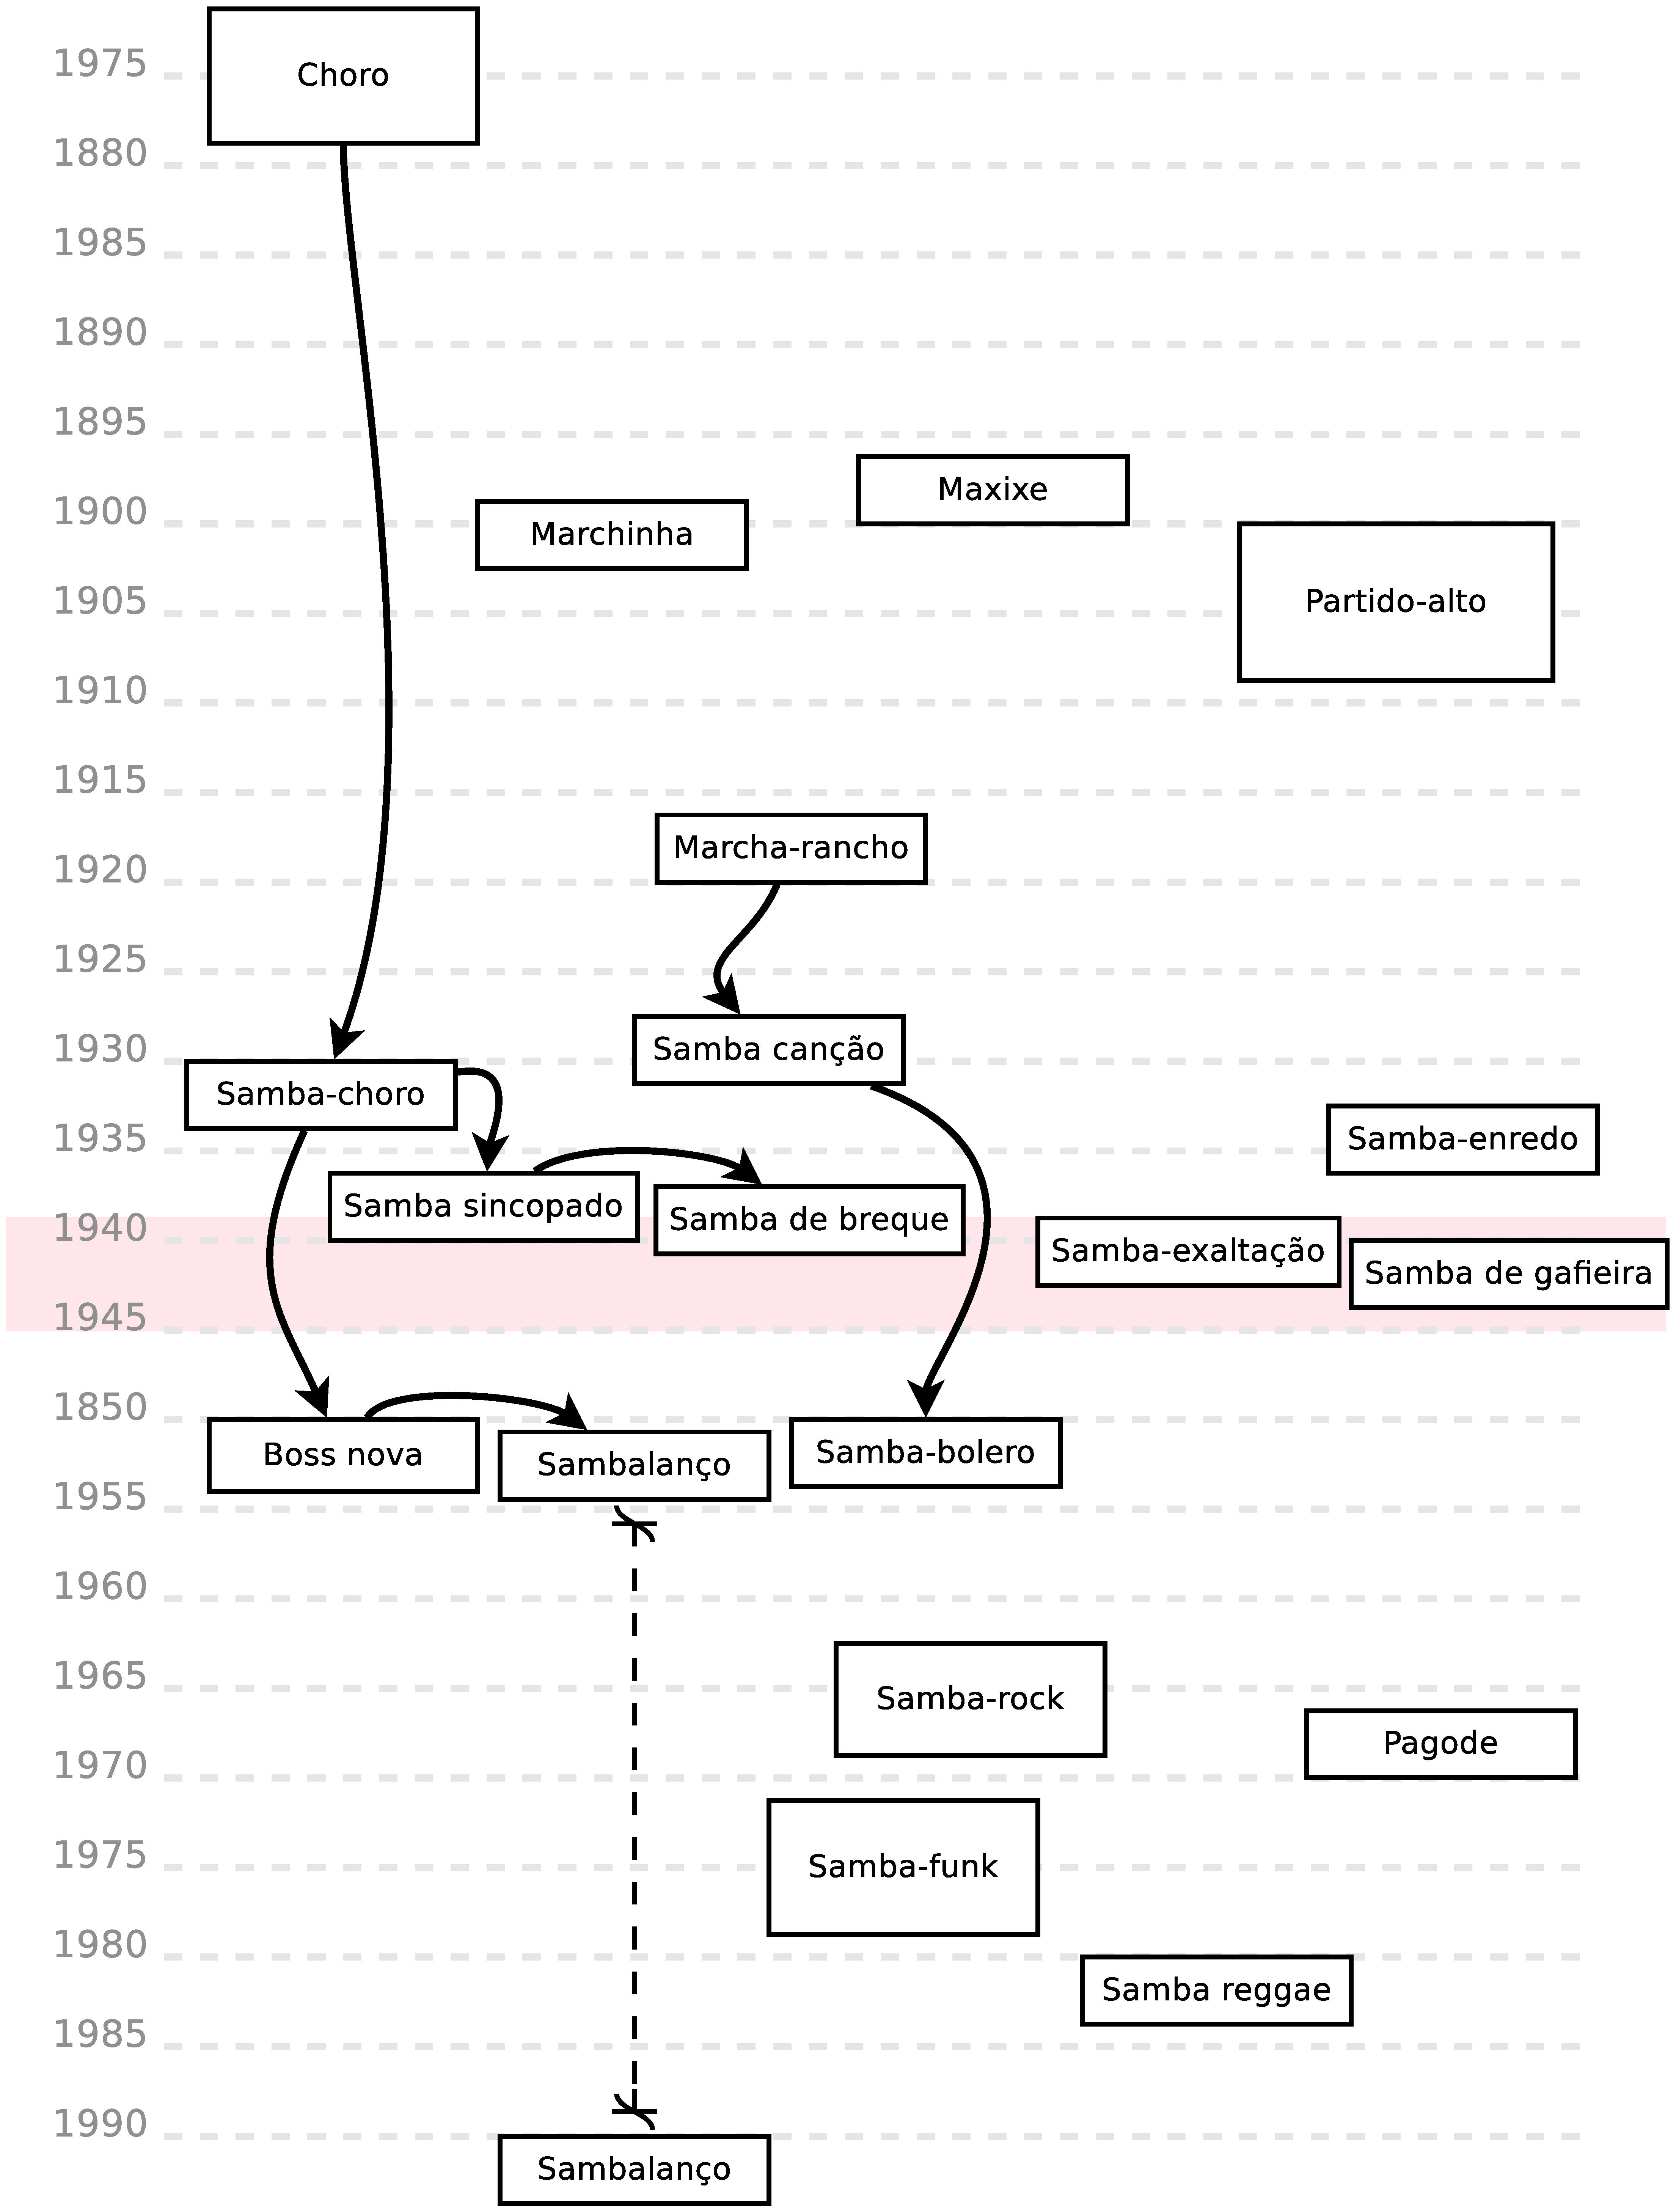
\includegraphics[width=0.95\textwidth]{chapters/cap-historia-musicasamba/musicatimeline.eps}
  \caption{Relação temporal entre os inícios dos subgêneros do samba.}
\label{fig:sambamusicatimeline1}
\end{figure}

%%%%%%%%%%%%%%%%%%%%%%%%%%%%%%%%%%%%%%%%%%%%%%%%%%%%%%%%%%%%%%%%%%%%%%%%%%%%%%%%
%%%%%%%%%%%%%%%%%%%%%%%%%%%%%%%%%%%%%%%%%%%%%%%%%%%%%%%%%%%%%%%%%%%%%%%%%%%%%%%%
\section{Que estilos de dança posso usar no samba (música)?}
\label{subsec:estilosdedanca}
A resposta mais simples poderia ser que, uma pessoa ao ser livre e independente,
pode escolher expressar-se na dança, de forma natural, como esta saia de si mesmo.
Porem, entrando em assuntos mais técnicos, 
e de acordo com os padrões socialmente mais comuns de ser achados atualmente;
existe um grupo de estilos de danças, que por suas caraterísticas, 
são consideradas que se enquadram muito bem na música de alguns subgêneros do samba.

Assim, nas seguintes seções, serão descritos alguns dos estilos de dança para a música do samba,  
que podemos achar nos salões e locais de dança no Brasil;
estes serão agrupados em estilos dançados em pares, e os que se dançam de forma separada. 


%%%%%%%%%%%%%%%%%%%%%%%%%%%%%%%%%%%%%%%%%%%%%%%%%%%%%%%%%%%%%%%%%%%%%%%%%%%%%%%%
\begin{comment}
\subsection{\textcolor{blue}{Estilos dançados em roda}}
\label{subsec:estilosdedancaroda}
Entre os estilos que se dançam em roda, temos:
\begin{description}
\item[Samba de roda:] Samba dançado em roda.
Para mais detalhes ir a página \pageref{ref:Samba-de-roda-danca}.

\item[Samba-de-umbigada:] 
São classificadas com este nome todas as danças que usem a umbigada na sua realização.
Para mais detalhes ir a página \pageref{ref:samba-de-umbigada}.

\item[Batuque (1900s):] Dança em roda onde se intercambiam os dançantes usando o gesto da umbigada.
Para mais detalhes ir a página \pageref{ref:batuquedanca}.

\item[Batucada:] Dança em roda onde se intercambiam os dançantes usando o gesto da pernada.
Para mais detalhes ir a página \pageref{ref:batucadadanca}.
\end{description}
\end{comment}
%%%%%%%%%%%%%%%%%%%%%%%%%%%%%%%%%%%%%%%%%%%%%%%%%%%%%%%%%%%%%%%%%%%%%%%%%%%%%%%%
\subsection{Estilos dançados em pares}
\label{subsec:estilosdedancapares}
Entre os estilos que se dançam a dois, existentes na atualidade, temos \cite[pp. 134]{perna2002samba}:
\begin{description}
\item[Samba de gafieira (dança):] 
\index{Dança!Samba de gafieira}
É uma dança a dois, que pode ser executada na maioria dos subgêneros do samba (música),
tendo exceções em: samba-enredo, samba reggae (música), samba rock (música), 
marcha, marcha-rancho e maxixe (música) \cite[pp. 134]{perna2002samba}.
No seus origens este tipo de dança era chamado de samba-batucada  \cite[pp. 134]{perna2002samba}. 
Para mais detalhes sobre o samba de gafieira, ver Seção \ref{subsec:gafieiradancaestilos}.

\item[Samba liso:] 
\index{Dança!Samba liso}
\index{Dança!Samba caminhado}
Atualmente se dança similarmente ao samba de gafieira, 
porem com um estilo mais elegante, sem ginga né passos de efeito, e dizer é uma dança mais ``lisa'';
se dança bem em : samba-canção, bossa nova e choro \cite[pp. 134]{perna2002samba}.

%%%%%%%%%%%%%%%%%%%%%%%%%%%%%%%
Podemos achar uma referencia interessante ao uso do termo \textbf{samba} e \textbf{liso}  no livro 
``Feitiço decente: Transformações do samba no Rio de Janeiro (1917-1933)'' (2001),
onde se pode intuir a procedência deste nome ou denominação, 
quando se faz referencia a um comentário de João da Baiana sobre o samba-de-umbigada e o samba de roda \cite[pp. 109]{sandroni2001feitico}: 
\begin{citando}
Nós tirávamos um verso e o pessoal sambava, um de cada vez ... 
Um saía para tirar o outro.
Se fosse a ``liso'' era só umbigada, mas se fosse para pegar ``duro'' já era capoiragem. 
\end{citando}
Pelo que no livro se comenta, que para o dançarino solista  escolher a seu sucessor podiam
existir duas modalidades, dependendo do tipo de roda, em ``samba liso'' (com umbigada) ou em ``samba duro'' 
(ou batucada\footnote{No qual a umbigada é substituída por uma pernada \cite[pp. 109]{sandroni2001feitico},
para mais detalhes ir a página \pageref{ref:batuquedanca}.}) \cite[pp. 109]{sandroni2001feitico}.
Esta referencia 
é particularmente interessante, pois como veremos na Seção \ref{cap:sambagafieira},
nos primórdios do samba nas gafieiras, existiam 3 formas em que esta era dançada: samba-canção (dança),
\textbf{samba-batucada} (dança)\footnote{Que 
é o nome com que era conhecido originalmente a atual samba de gafieira \cite[pp. 143]{perna2002samba}.} 
e \textbf{samba-liso} \cite[pp. 143]{perna2002samba};
estas duas últimas, não são as mesmas danças dos samba-de-umbigada, 
e sim novas formas de dançar o samba num ambiente mais civilizado como o salão de dança;
porem, estes nomes conservavam a mesma nomenclatura, na descrição 
da relativa relação à tosquedade dos movimentos.

%%%%%%%%%%%%%%%%%%%%%%%%%%%%%%%
Na ``Hemeroteca Digital Brasileira'' da Fundação Biblioteca Nacional,
não tem-se achado referencias\footnote{ Foram achadas,
2, 5, 3, 1 e 1 referencias brutas para as décadas de 1930, 1940, 1960, 1970 e 1980 respetivamente;
porem, estas não eram relativas ao samba liso de salão ou eram falsos acertos.} 
à frase ``\textbf{samba liso}'', nas décadas de 1930, 1940, 1960, 1970 e 1980;
as referencias achadas correspondem à década de 1950\footnote{Especificamente entre os anos 1950 e 1953.}  
com uma total de 327 referencias;
de todas estas, 326 correspondem à forte campanha 
de marketing do livro
``Como aprender a dançar'' , 
de Gino Forniciari. 
Por exemplo, podemos achar a primeira referencia em ``O Jornal'' (RJ),
do dia 17 de setembro de 1950, onde se pode ler \cite[3ra seção pp. 9]{jornalanunciodanca1}:
\begin{citando}
\begin{center}
Como aprender a dançar\\
4a edição ampliada
\end{center}
Com a nova dança, ``Baião'', \textbf{Samba liso}, e os
últimos passos de Bolero, Rumba, Swing, contendo
120 gráficos 330 passos, facilitando as senhoritas 
e cavalheiros a aprenderem em suas próprias 
casas em 10 dias apenas, no princípio sem
companheiro ou companheira. Método de ritmos modernos
pelo Prof. Gino Fornaciari, 
Diretor e Prof. do ``CURSO PRATICO DE DANÇAS RITZ''.
Aulas particulares, rua da Liberdade, 120.
Preço: Cr\$ 45,00 -- Pedidos pelo reembolso posta 
-- com o autor -- Caixa Postal, 649 -- SÃO PAULO 
\end{citando}
Todos estes anúncios vem na maioria das vesses acompanhados com um desenho como
o mostrado na Figura \ref{fig:desenholivrodanca1}, que indica todos os estilos de dança abordados no livro;
onde se diferencia entre dançar \textbf{samba} e \textbf{samba liso}.
\begin{figure}[h]
  \centering
    \includegraphics[width=0.5\textwidth]{chapters/cap-historia-musicasamba/comoaprenderdancar.jpg}
  \caption{Desenho da publicidade do livro ``Como aprender a dançar'' de Gino Forniciari,
publicado, no dia 17 de fevereiro de 1952, em ``Sport Ilustrado'' \cite[pp. 22]{sportlivropublidanca}.}
\label{fig:desenholivrodanca1}
\end{figure}



%%%%%%%%%%%%%%%%%%%%%%%%%%%%%%%
A outra referencia achada na ``Hemeroteca Digital Brasileira'' da Fundação Biblioteca Nacional,
apara a frase ``samba liso'', na década de 1950, foi a publicada o dia 26 de agosto de 1951,
no ``Diário do Nordeste'' de Caixas do Sul (RS), numa cronica de Walter Brugger da sua viagem por Europa,
num articulo titulado ``Genova! Primeiro Contato com a Europa!'',
onde se pode ler \cite[pp. 10]{nordestesambalisocronica}:
\begin{citando}
Ao nosso lado, numa área 
descoberta uma orquestra tocava para
quem quizesse dançar.
Repentinamente ouvimos uma melodia muito
nossa conhecida. Era o imortal ``Tico-Tico no Fubá''... Todavia,
apesar da melodia correta, o ritmo
era bastante falho. Continuando 
com os ritmos brasileiros, a orquestra 
tocou ainda ``Chiquita Bacana'',
mas em tempo de samba e ``Aquarela do Brasil''.
O que porém nos 
deixou mais atônitos foi o modo como 
era dançado o nosso samba. De 
brasileiro não tinha nada. Pelo que 
vimos, o \textbf{samba ``liso''} lhes é desconhecido 
e cada um procura ``requebrar'' o corpo mais que o outro,
mas de uma forma como nós só 
conhecemos no cinema mexicano. 
O meu amigo dava gostosas risadas e não era para menos,
ante a comicidade do espetáculo, tão 
impossível no Brasil quanto desconhecido para nós.
\end{citando}


%%%%%%%%%%%%%%%%%%%%%%%%%%%%%%%
Outra referencia ao \textbf{samba liso}, pode ser achada no livro ``Manual de Danças Gaúchas'' (1955)
onde se afirma que \cite[pp. 77]{cortesmanual}: 
\begin{citando}
A polquinha, como dança especifica, é executada por pares enlaçados,
mediante passos-de-marcha (É correograficamente  semelhante ao chamado 
\textbf{samba liso} ou \textbf{samba caminhado} dos salões urbanos).
\end{citando}


\item[Samba pagode:] 
\index{Dança!Samba pagode}
É um estilo de dança a dois, originário de São Paulo, 
é uma dança com poucos deslocamentos \cite[pp. 134]{perna2002samba}.
É um estilo de dança adaptado para ser dançado com o pagode paulista,
também chamado como Sambalanço\footnote{Ver página \pageref{ref:sambalanco}}.
%% https://www.youtube.com/watch?v=SfvoiXOGPn4
Ao igual que o sambalanço teve duas épocas com estilos musicais diferentes,
a dança \textbf{samba pagode}, sofreu também transformações acompanhando essas tendencias.
Podem-se observar atualmente 3 tipos de passo base: 
%% https://www.youtube.com/watch?v=rq1uhNXySds 
%% https://www.youtube.com/watch?v=SfvoiXOGPn4

O miudinho, que é um passo que se realiza abraçado com o par e de forma espelhada com este,
onde se executam 3 twist\footnote{É importante ter um sapato que deslise bem.} no lugar, 
só trocando de peso entre os pés, seguindo um ritmo, rápido-rápido-lento;
este movimento se executa simetricamente duas vesses para formar um ciclo completo,  
uma vez iniciando com o peso do corpo para o pé direito\footnote{Quando o primeiro twist é horário.} e a outra com o esquerdo.

O passo básico lateral, se realiza abraçado com o par  e de forma espelhada com este, 
é similar ao passo básico de capoeira,
ou a base aberta do forró\footnote{Só que aqui é abraçados.},
onde se produzem 3 movimento seguindo um ritmo, rápido-rápido-lento,
no primeiro momento, um pé vai para atrás, 
no segundo o outro ajeita sua posição deslocando-se levemente, 
procurando o centro e o equilíbrio do par dançante, e
no terceiro o pé que estava atrás volta ao lado do outro,
este movimento se executa simetricamente duas vesses para formar um ciclo completo,  
uma vez iniciando com pé direito e a outra com o esquerdo.
Este movimento é interessante para fazer deslocamento, 
que são realizados principalmente nesse primeiro movimento com o pé atrás, 
só que agora apontando para uma direção especifica.

A caidinha, se realiza abraçado com o par, 
este passo é similar ao picadilho (picadinho) de samba de gafieira,
porem com um deslocamento similar ao repique do forró;
no pagode paulista este movimento se executa seguindo um ritmo, rápido-rápido-lento,
onde o seguidor faz um movimento similar ao miudinho antes mencionado,
enquanto que o condutor tem uma liberdade criativa no 
seu movimento\footnote{O mesmo que acontece no picadilho de samba de gafieira.} 
enquanto respeite o ritmo, rápido-rápido-lento.


\item[Samba rock:] 
\index{Dança!Samba rock}
É um estilo de dança a dois, realizado nos bailes ``black'' paulistas desde a década de 1960, 
sendo esta uma dança variante das danças do swing/rock e parente do soltinho carioca \cite[pp. 135]{perna2002samba}.
se dança bem em: Swing, samba rock (música), samba com suingue e samba-funk \cite[pp. 135,138]{perna2002samba}.
O samba rock se dança de mão dadas, e se carateriza por ter muitas voltas,
executadas na maior parte de vesses pelas  seguidores;
porem, é uma dança estacionaria pois os dançantes rara vez se deslocam pelo salão, 
e pelo contrario ficam trabalhando seus passos num mesmo lugar  \cite[pp. 135,138]{perna2002samba}.
Quando um espectador externo vê esta dança perceberá muitas figuras usando só os braços,
com enrosques, voltas, enlaces, etc.
Enquanto os pés de ambos dançarinos fazem uma mesma marcação, num constante e repetitivo rápido-rápido-lento,
caminhando unicamente sobre um circulo imaginário no chão, uma vez em sentido horário e outra em anti-horário.

\item[Samba funkeado:] 
\index{Dança!Samba funkeado}
Também é chamado de estilo Jimmy de Oliveira ou simplesmente  samba Jimmy, 
em aluição a seu criador.
Este estilo de dança a dois foi criado no ano de 1998.
Com muito esforço Jimmy, num período aproximado de 6 meses, 
criou a estrutura da dança, desde iniciante ate avançado;
no ano de 1999 ele  chamou a esse estilo como ``samba quebrado'';  
posteriormente renomeou  para ``samba Jimmy'', 
recebeu algumas criticas e no ano 2001 decidiu renomeá-lo para ``samba funk'',
porem isto trouxe confusões   ao ser associado com a música funk, existente em Rio de Janeiro,
muito distante da proposta dele, e
finalmente a meados do 2005 ele decidiu chamá-lo ``samba funkeado''  \cite{sambafunkeadoJimmyDeOliveiraPart1}.
A Figura \ref{fig:funkeadocrono1} mostra a cronologia de nomes para este estilo.
\begin{figure}[h]
  \centering
    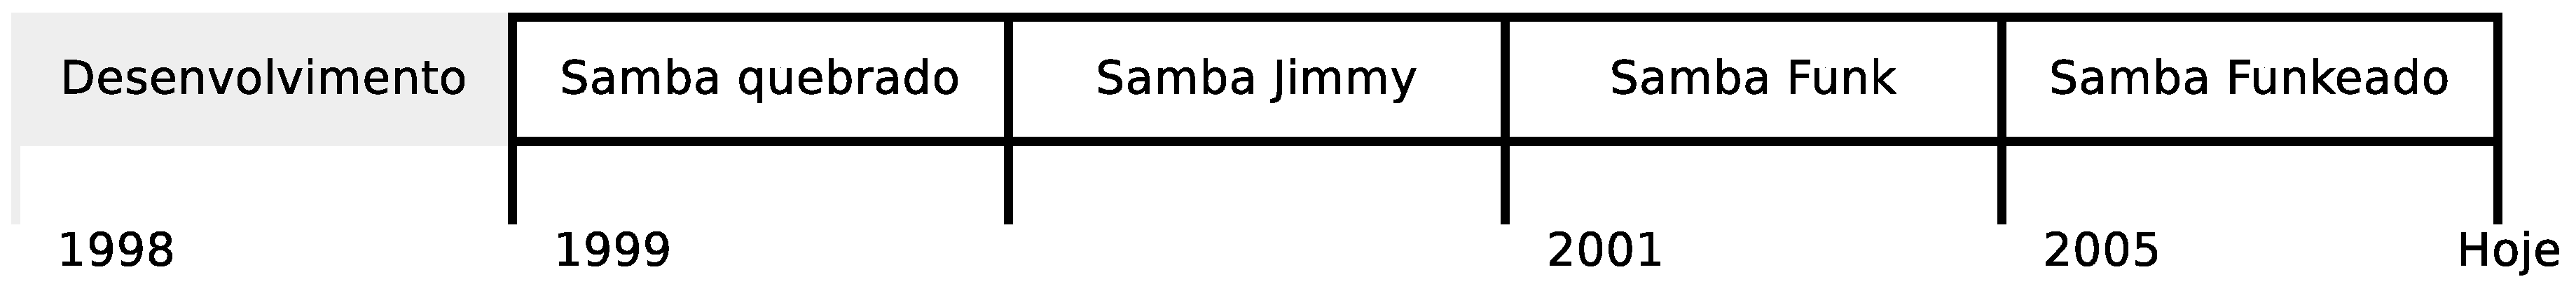
\includegraphics[width=0.85\textwidth]{chapters/cap-historia-musicasamba/sambafunkeado.eps}
  \caption{Cronologia dos nomes para samba funkeado.}
\label{fig:funkeadocrono1}
\end{figure}

O estilo foi criado para, em palavras de Jimmy: ``contribuir em função da música'', 
numa tentativa de agregar movimento em coerência como as músicas que ele gostava;
sendo estas interpretadas por:
Djavan, Jorge Ben Jor, Tim Maia, Leny Andrade \cite{sambafunkeadoJimmyDeOliveiraPart1}, que em seu momento, 
presentaram músicas de bossa nova ou que eram influenciadas pelo jazz, funk norte-americano ou ``black music'' \cite{sambafunkeadoJimmyDeOliveiraPart1} \cite{sambafunkeadoJimmyDeOliveiraPart3},
Jimmy indica que seu estilo procura ir em função da música escutada no brasil, 
e que a maioria da música atual é influenciada pelo funk norte-americano;
como a música de: João Sabiá. 

O samba funkeado pode ser dançado em gêneros como ``black music'',
em pagodes funkeados (Sorriso maroto, Netinho de Paula, pixote, etc.), em sambas com influencia do jazz \cite{sambafunkeadoJimmyDeOliveiraPart3}, etc. 

O samba funkeado tem 3 tendencias ou estruturas  \cite{sambafunkeadoJimmyDeOliveiraPart2}:
\begin{itemize}
\item \textbf{Samba funkeado}, primigênio.
\item \textbf{Samba funkeado fragmentado}; exemplo: um movimento que é de sentar, que gastaria um tempo, 
passa a ter ate 3 tempos; é dizer, fragmenta os movimentos. 
O fragmentado também permite dançar com movimentações em contrapeso no par de dança.
\item \textbf{Samba funkeado samsurf}, com uma postura mais curvada.
\end{itemize}

%e em seu ídolo Michael Jackson \cite{sambafunkeadoJimmyDeOliveira2}.
 

\item[Samba internacional:] 
\index{Dança!Samba internacional}
É um estilo de dança a dois, influenciado pelo maxixe;
se dança principalmente fora do Brasil e existem basicamente dois estilos: 
o estilo internacional e o estilo norte-americano (EE.UU.) \cite[pp. 134-135]{perna2002samba}.

O samba introduzida a EE.UU. é uma dança de salão muito animada, 
com música de ritmo alegre, que sugere um estilo de movimento que pode
chegar a ser tão turbulento quanto os movimentos do Jive.
O padrão de passos básicos é similar aos achados no Fox-Trot e o Waltz,
sendo estes: fwd-swd-close ... bwd-swd-close; e
tem passos com tempos que seguem uma sequência: 
quick-quick-slow\footnote{Rápido-rápido-lento.} ... quick-quick-slow \cite{parson2016ballroom}.

Observando os campeonatos internacionais onde este estilo é usado, 
se percebe que o samba internacional é dançado em qualquer estilo musical que
tenha sotaque ou de a impressão de ter raiz afro-latina.

\end{description}~

A Figura \ref{fig:sambadavavsmusica} mostra as relações entre os estilos de dança a dois atuais,
 e os subgêneros do samba \cite[pp. 134-138]{perna2002samba}.

\begin{figure}[h]
  \centering
    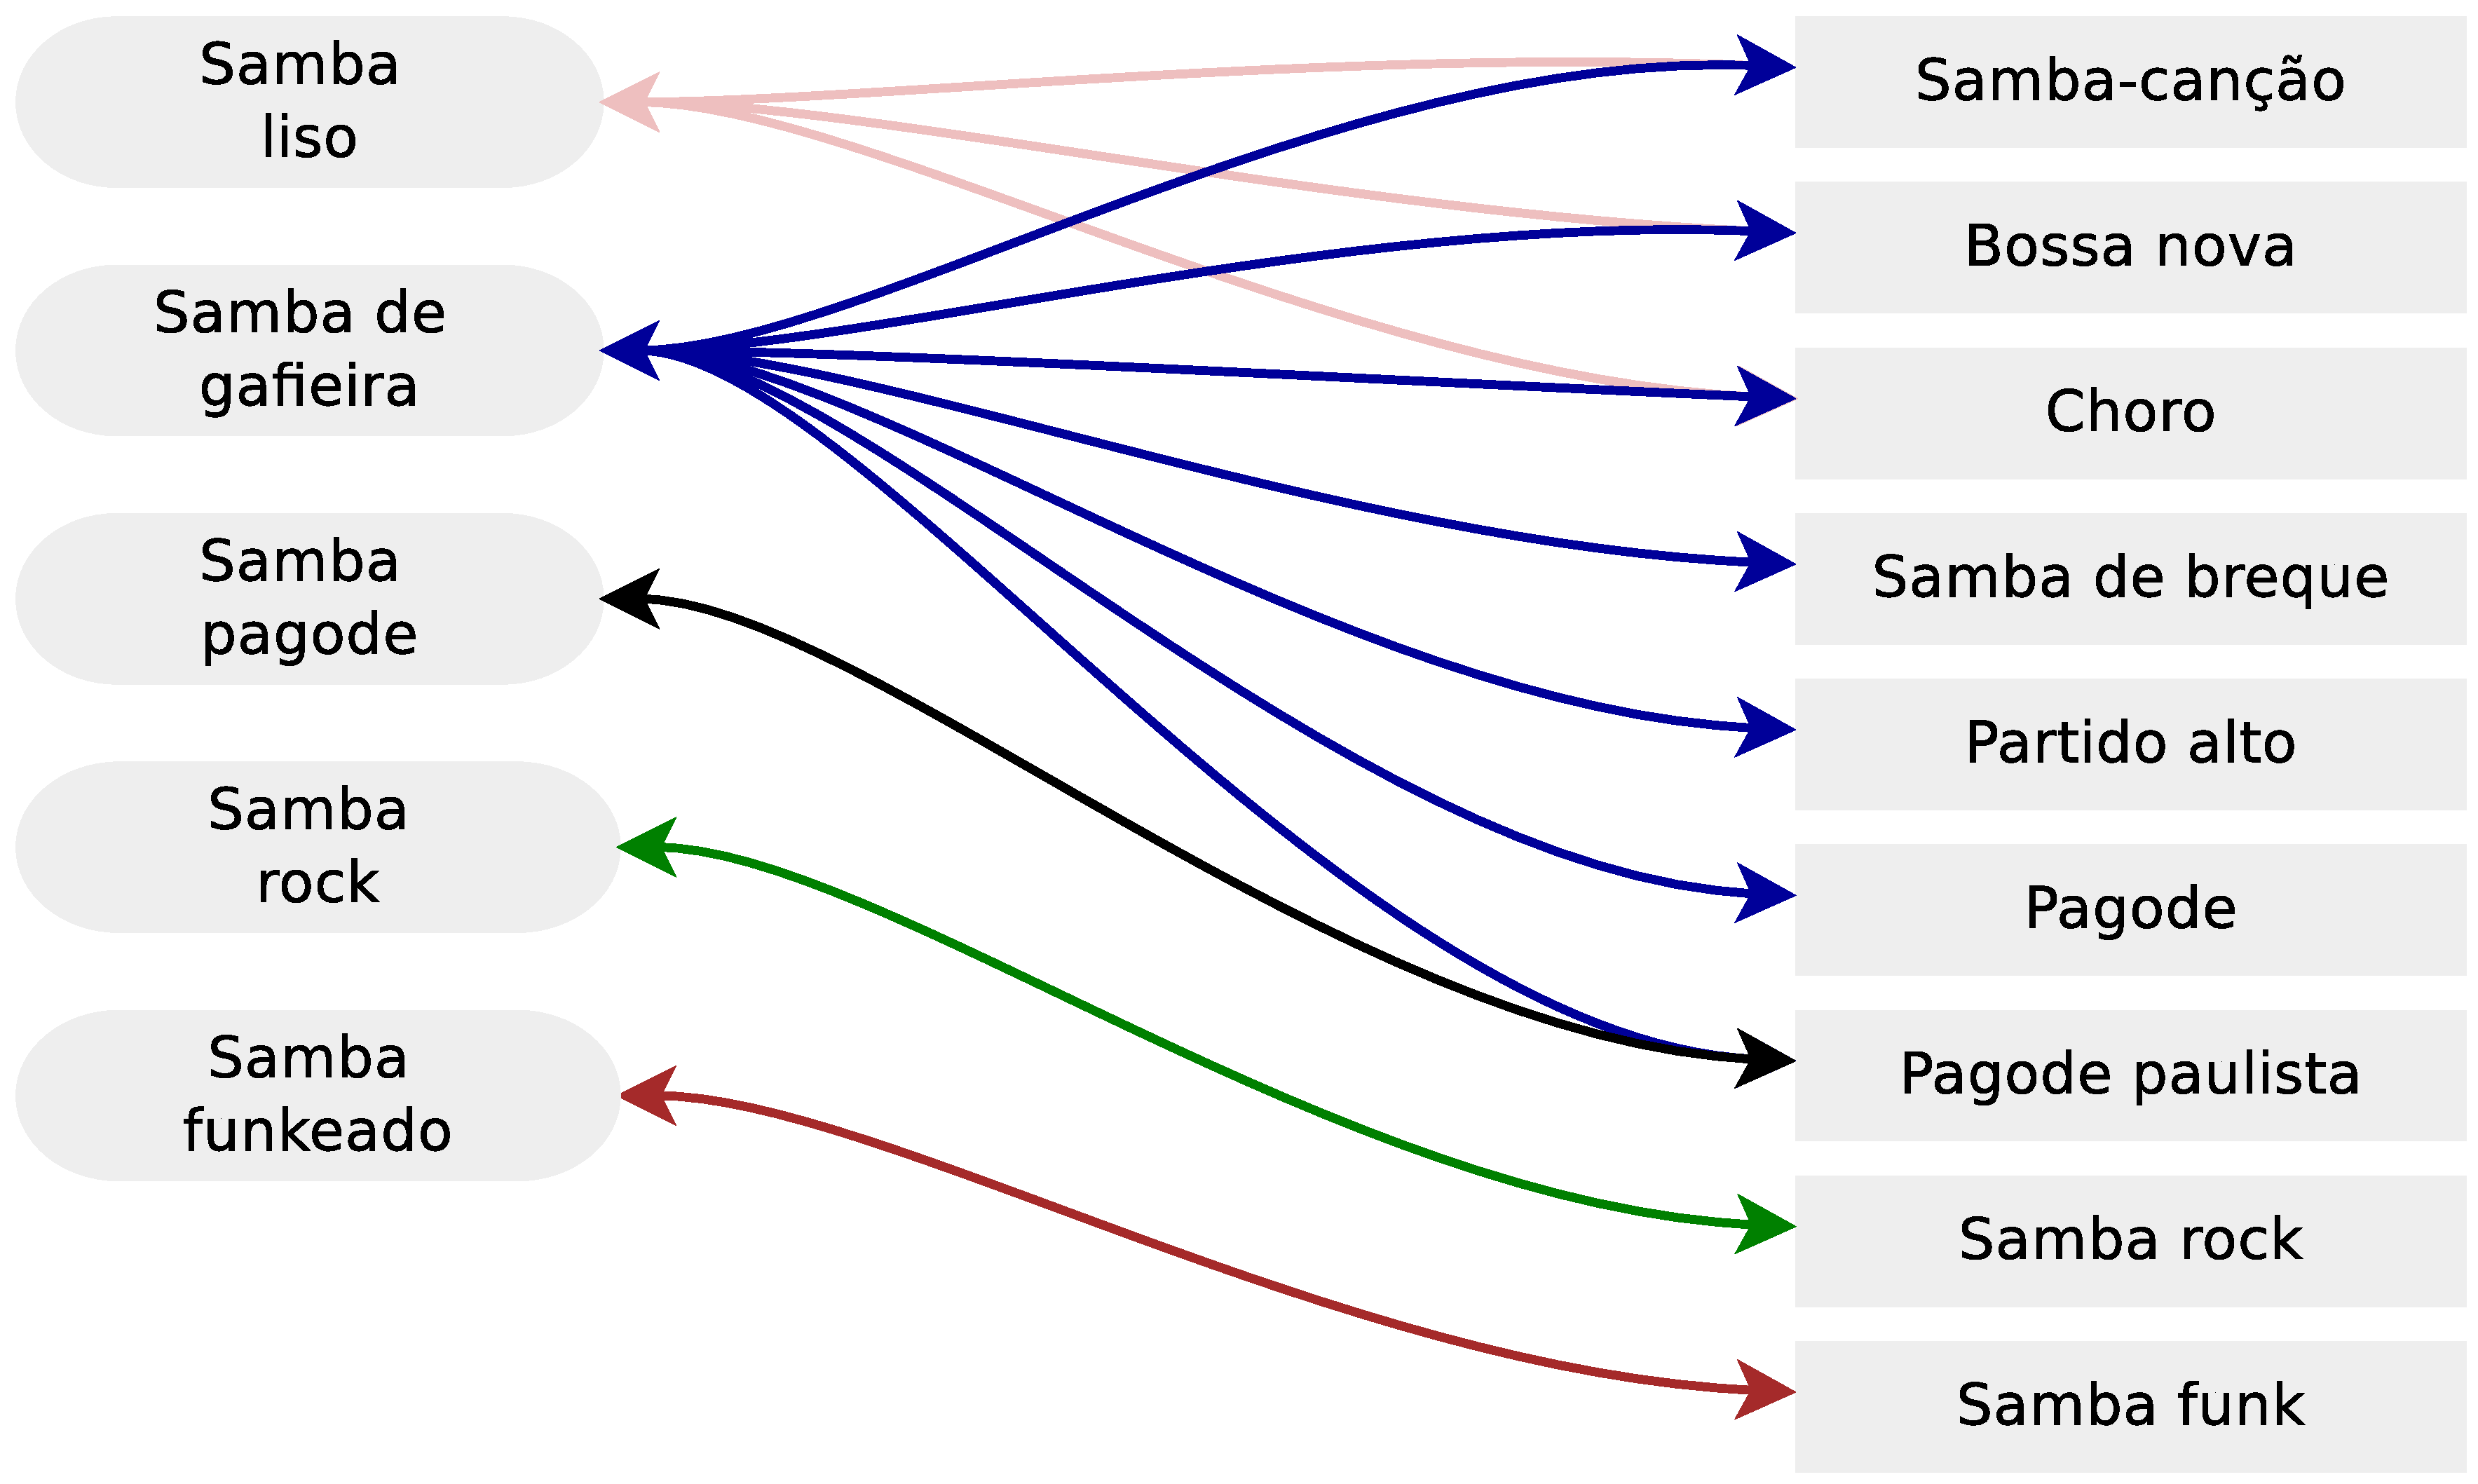
\includegraphics[width=0.6\textwidth]{chapters/cap-historia-musicasamba/dancavcmusica.eps}
  \caption{Relações entre os estilos de dança a dois e os subgêneros do samba.}
\label{fig:sambadavavsmusica}
\end{figure}

%%%%%%%%%%%%%%%%%%%%%%%%%%%%%%%%%%%%%%%%%%%%%%%%%%%%%%%%%%%%%%%%%%%%%%%%%%%%%%%%
\subsection{Estilos dançados individualmente ou separados }
Entre os estilos que se dançam de forma separada temos \cite[pp. 134]{perna2002samba}:
\begin{description}
\item[Samba reggae  (dança):] Este estilo de samba que se dança separado, 
é uma dança baiana também conhecida como axé-dance, samba baiano ou pagode baiano,
se dança em samba reggae (música) \cite[pp. 134]{perna2002samba}.

\item[Samba no pé:] É o estilo usado nas quadras das escolas de samba,
se dança bem em estilos musicais como: 
samba enredo ou em qualquer samba rápido  \cite[pp. 134]{perna2002samba}.

\item[Marcha de carnaval:] É uma dança própria do carnaval para se dançar em cordões.
se dança bem em: marchas, marchas-rancho e samba-enredo lentos  \cite[pp. 135]{perna2002samba}.

\end{description}
~

A Figura \ref{fig:sambadavavsmusicaseparado} mostra as relações existentes, 
entre os estilos de dança que se dançam separados e alguns subgêneros do samba  \cite[pp. 134-138]{perna2002samba}.

\begin{figure}[h]
  \centering
    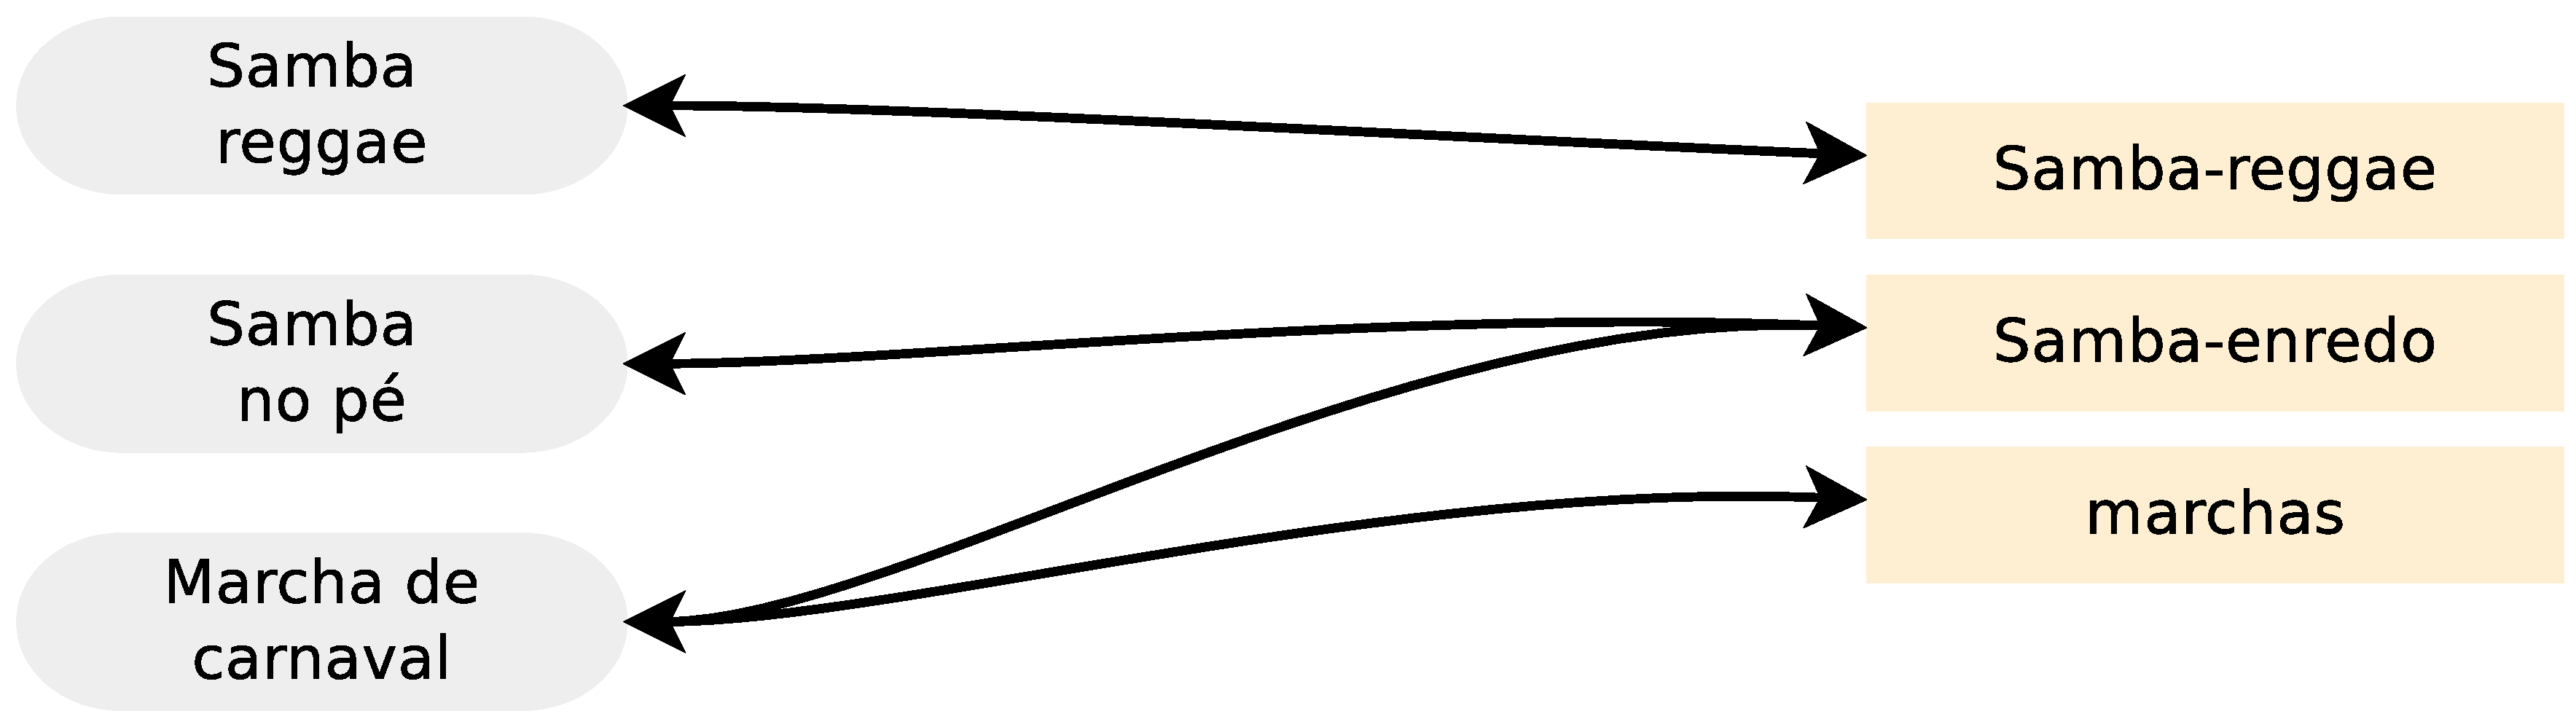
\includegraphics[width=0.6\textwidth]{chapters/cap-historia-musicasamba/dancavcmusicaseparado.eps}
  \caption{Relações entre os estilos de dança (separados) e os subgêneros do samba.}
\label{fig:sambadavavsmusicaseparado}
\end{figure}


%%%%%%%%%%%%%%%%%%%%%%%%%%%%%%%%%%%%%%%%%%%%%%%%%%%%%%%%%%%%%%%%%%%%%%%%%%%%%%%%
%% CAPITULO
%%%%%%%%%%%%%%%%%%%%%%%%%%%%%%%%%%%%%%%%%%%%%%%%%%%%%%%%%%%%%%%%%%%%%%%%%%%%%%%%
\chapterimage{chapter_head_2.pdf} % Chapter heading image

\chapter{\textcolor{green}{Historia do samba de gafieira  (dança)}}
\label{cap:sambagafieira}
\index{Dança!Samba de gafieira}


\section{Lundum (a dança do lundu)} 
\label{sec:lundu}
\index{Dança!Lundu}
O lundum é o estilo de dança que lhe corresponde ao gênero musical lundu \cite[pp. 18]{perna2002samba}.
Esta é uma dança, brasileira, de roda e umbigada; e teve sua origem no batuque dos bantos africanos,
e provavelmente foi trazida de Angola pelos escravos na segunda metade do século XVIII \cite[pp. 48]{tinhorao1986pequena} \cite[pp. 188]{dourado2004dicionario},
sendo que as primeiras referencias conhecidas se remontam a 1780 
descrevendo a dança como indecente e licenciosa \cite[pp. 51]{tinhorao1986pequena} \cite[pp. 19]{perna2002samba}.
Posteriormente foi introduzida aos salões das cortes do Brasil e Portugal, 
dançado elegantemente nas cortes, porem indecentemente pela gente comum   \cite[pp. 19]{perna2002samba} \cite[pp. 188]{dourado2004dicionario}.
No Brasil esta dança teve influencias da ``Modinha''(Portuguesa) e do ``Fandango''(Espanhol) \cite[pp. 188]{dourado2004dicionario}.

A partir de 1820 o lundum é apresentado, como dança de caráter libidinoso nos teatros de Baia, Pernambuco e Rio de Janeiro;
onde eram representados pequenos quadros cômicos, 
mostrando a umbigada e outras caraterísticas da dança \cite[pp. 19]{perna2002samba}.


\section{Maxixe (dança)}
\label{sec:maxixe}
\index{Dança!Maxixe}
Esta é uma dança urbana afro-brasileira \cite[pp. 4]{musicasambavariasdef1}, 
em compasso binário, surgida em Rio de Janeiro, 
na Cidade Nova e nos cabarés de Lapa \cite[pp. 465]{marcondes1977enciclopedia}  \cite[pp. 198]{dourado2004dicionario}, 
aproximadamente entre 1870 e 1880 \cite[pp. 58]{tinhorao1986pequena} \cite[pp. 465]{marcondes1977enciclopedia}  \cite[pp. 62]{reinato2010musica}.

A dança era considerada de baixe ralé pela sociedade local, 
pois era entendida como um modismo indecente das classes baixas, imoral como o Lundu \cite[pp. 198]{dourado2004dicionario}.
Esta dança recebeu influencias da polca \cite[pp. 198]{dourado2004dicionario} e 
da Habanera \cite[pp. 62]{reinato2010musica}.


O maxixe tinha uma boa quantidade de passos como: 
\begin{itemize} 
\item parafuso  \cite[pp. 68, 93, 129]{efege1974maxixe} \cite[pp. 465]{marcondes1977enciclopedia} \cite[pp. 62]{tinhorao1986pequena}, 
\item janela  \cite[pp. 129]{efege1974maxixe},
\item jocotó \cite[pp. 83, 96, 173]{efege1974maxixe},
\item saca-rolha \cite[pp. 465]{marcondes1977enciclopedia}, 
\item balão \cite[pp. 93]{efege1974maxixe} \cite[pp. 465]{marcondes1977enciclopedia}, 
\item balão apagado \cite[pp. 68]{efege1974maxixe} \cite[aproximadamente min. 11:35]{MaxixeDocumentario1},
\item balão caindo  \cite[pp. 129, 131]{efege1974maxixe} \cite[pp. 62]{tinhorao1986pequena},
\item corta-jaca  \cite[pp. 131]{efege1974maxixe},
\item urubu malandro  \cite[pp. 131]{efege1974maxixe},
\item sino \cite[pp. 68]{efege1974maxixe}, 
\item carrapeta  \cite[pp. 465]{marcondes1977enciclopedia}, 
\item corta-capim \cite[pp. 465]{marcondes1977enciclopedia} \cite[pp. 62]{tinhorao1986pequena}, 
\item cobrinha \cite[pp. 62]{tinhorao1986pequena},
\item maxixe puladinho \cite[pp. 177]{1920revista},
\item etc. 
\end{itemize}
Num principio o maxixe era dançado nas músicas de tango, havanera, polca e lundu; 
e só foi ate o final do século XIX que ganhou uma música com gênero próprio \cite[pp. 465]{marcondes1977enciclopedia},
criado pela fusão da polca, o schottisch e a mazurca \cite[pp. 58]{tinhorao1986pequena}.

No inícios do século XX o maxixe foi exportado e dançado na Europa, atingindo um grande sucesso, 
chegando a ser apresentado pelo dançarino ``Duque'' em Paris (1914) e em Londres (1922) \cite[pp. 465]{marcondes1977enciclopedia}.
Este dançarino é considerado o civilizador do maxixe \cite[pp. 129]{efege1974maxixe}.

Uma explicação muito interessante do maxixe é cantada pela atriz, Aurélia Delorme,
numa representação num quadro de revista, interpretando  ``Maxixe Aristocrático'' (1904, José Nunes), 
que arrancava aplausos e provocava pedidos de bis;
o seguinte texto indica sua pauta \cite[pp. 80-81]{efege1974maxixe} \cite{REIS2003}: 
\begin{citando}
O maxixe tem ciência,\\
ou pelo menos tem arte.\\
Para haver proficiência\\
basta mexer certa parte.\\
Pois o próprio Padre Santo,\\
sabendo o gosto que tem,\\
virá de Roma ao Brasil\\
dançar maxixe também.\\ 
\end{citando}



\section{\textcolor{green}{Samba de gafieira (dança)}}
\index{Dança!Samba de gafieira}
O samba de gafieira, como dança, descende principalmente do maxixe (dança),
que a sua vez foi gerado  pela união do  lundu, 
a polca e outras danças europeias.
Assim, misturando o maxixe com a ginga, e o ritmo de outras danças africanas, 
é que se obteve o que agora chamaríamos como samba de gafieira (primigênio)\footnote{
Primitivo; primordial; o primeiro da sua espécie. = PRIMÍGENO \cite{priberamprimigenio}.
} \cite[pp. 139]{perna2002samba}.




A Figura \ref{fig:formuladosambagafieira} mostra a árvore genealógico do samba de gafieira (primigênio),
visto quando o samba fez sua aparição nos salões de dança denominados gafieiras.
\begin{figure}[h]
  \centering
  \begin{subfigure}[b]{0.535\textwidth}
    \centering
    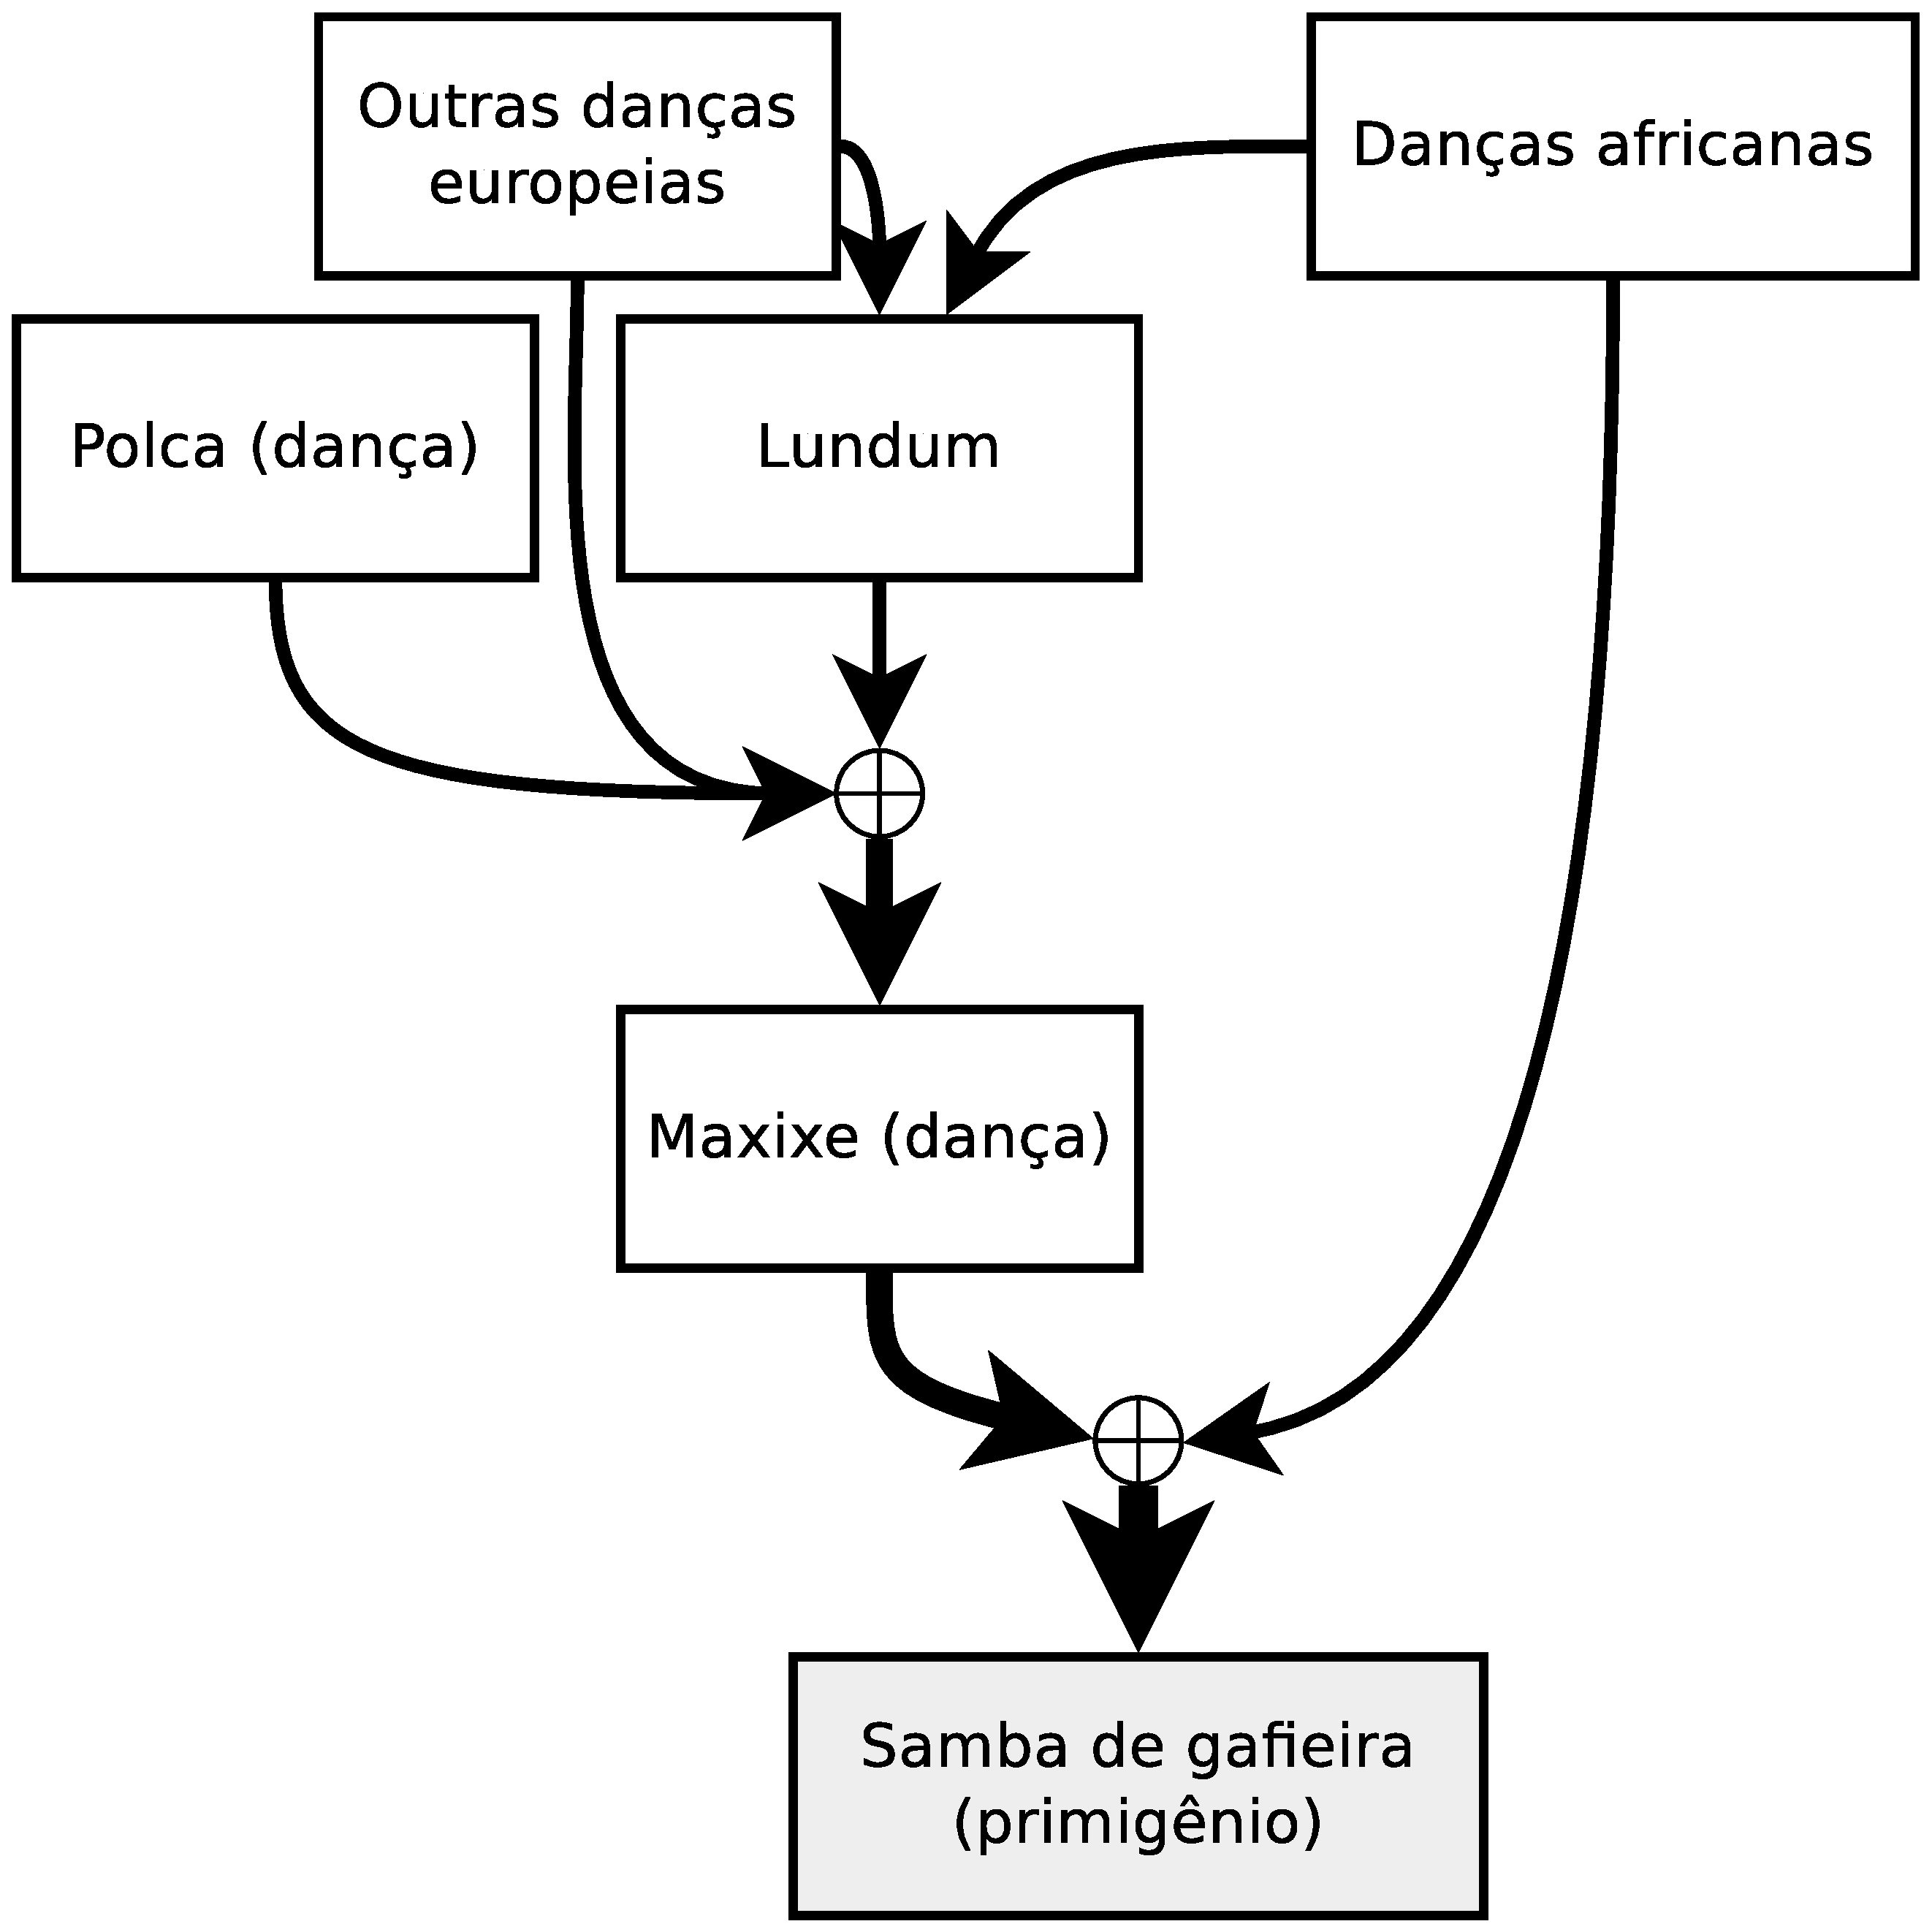
\includegraphics[width=\textwidth]{chapters/cap-historia-sambagafieira/sambagafieiraformula.eps}
    \caption{Formação do samba de gafieira (primigênio).}
    \label{fig:formuladosambagafieira}
  \end{subfigure}
  \begin{subfigure}[b]{0.385\textwidth}
    \centering
    \includegraphics[width=\textwidth]{chapters/cap-historia-sambagafieira/sambagafieiraformula2.eps}
    \caption{Formação do samba de gafieira (atual).}
    \label{fig:formuladosambagafieira2}
  \end{subfigure}
\caption{Formula da criação do samba de gafieira.}
\label{fig:formuladosambagafieiraall}
\end{figure}


O aparecimento do samba nos salões de dança, 
foi um grande impacto para as pessoas que frequentavam estes lugares;
sendo considerado um ritmo novo e ligeiro,
que desagradou aos bailarinos de maior idade e menos ágeis \cite[pp. 6 - cad. B]{entrevistajuliojournalbrasil1}.
O senhor, Júlio Simões, Administrador da ``Kananga do Japão'' e posteriormente socio
do ``Elite Club'', chegou a temer pelo futuro do seus empreendimentos; porem, para sorte dele, 
o samba fez muito sucesso no Elite,
e passou a ser considerado vestibular indispensável para qualquer pessoa que pretendesse ser bailarino, 
compositor ou instrumentista \cite[pp. 6 - cad. B]{entrevistajuliojournalbrasil1}.

\PRLsep{Samba nos salões em 1940}

Pode-se estabelecer o ingresso do samba, aos salões de dança, entre os anos de 1930 e 1940 \cite[pp. 140]{perna2002samba}.
Em palavras do Prof. de dança Gino Fornaciari, 
o samba dessa época tinha um aprecido com o Foxtrot e a Rumba, se dançava num compasso binario,
sendo esta dança a preferida do mulato brasileiro
%sendo este estilo de dança de salão que nasceu na \hyperref[ref:batucadadanca]{\textbf{batucada}} 
%de pretos que descia à cidade na epoca das festas 
\cite[pp. 50]{fornaciari1947aprender}.
Para a decada de 1940 o samba carioca de salão \cite[pp. 50]{fornaciari1947aprender},  já tinha ganhado muita força nos salões,
e podia-se ver 3 modalidades de dançar o samba \cite[pp. 58]{freitas1959danca} \cite[pp. 142-143]{perna2002samba} 
\cite[pp. 51]{fornaciari1947aprender}:
\begin{itemize}
\item \textbf{Samba-canção (dança)},
\index{Dança!Samba-canção} 
Era uma dança com balanços aos lados que se executava de joelhos flexionados,
usando dois movimentos por cada compasso binario \cite[pp. 58]{freitas1959danca} 
\cite[pp. 51]{fornaciari1947aprender} \cite[pp. 143]{perna2002samba}; 
na atualidade é um modo de dança extinto \cite[pp. 143]{perna2002samba}.

Sobre os passos usados entre 1947-1959, 
na Figura \ref{fig:samba-cancao-basico-frente} se mostra o passo básico para a frente do samba-canção,
e na  Figura \ref{fig:samba-cancao-basico-frente} o mesmo movimento para trás;
em ambos casos se usa os 2 movimentos antes mencionados, e a cor cinza indica a posição inicial \cite[pp. 51]{fornaciari1947aprender} \cite[pp. 59-60]{freitas1959danca}. 
\begin{figure}[h]
    \centering
    \begin{subfigure}[b]{0.4\textwidth}
        \centering
        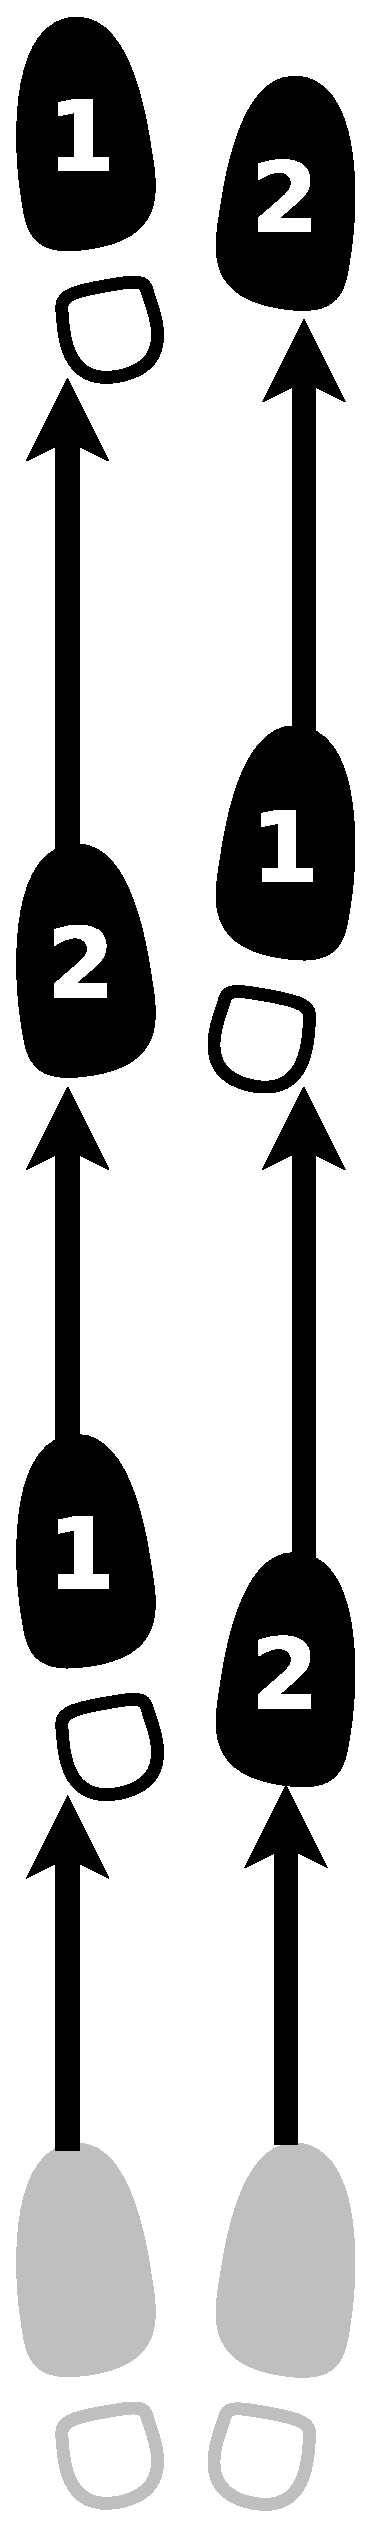
\includegraphics[width=0.25\textwidth]{chapters/cap-historia-sambagafieira/samba-cancao-basico-frente.eps}
        \caption{Passo básico para a frente.}
        \label{fig:samba-cancao-basico-frente}
    \end{subfigure}
    ~ %add desired spacing between images, e. g. ~, \quad, \qquad, \hfill etc. 
      %(or a blank line to force the subfigure onto a new line)
    \begin{subfigure}[b]{0.4\textwidth}
        \centering
	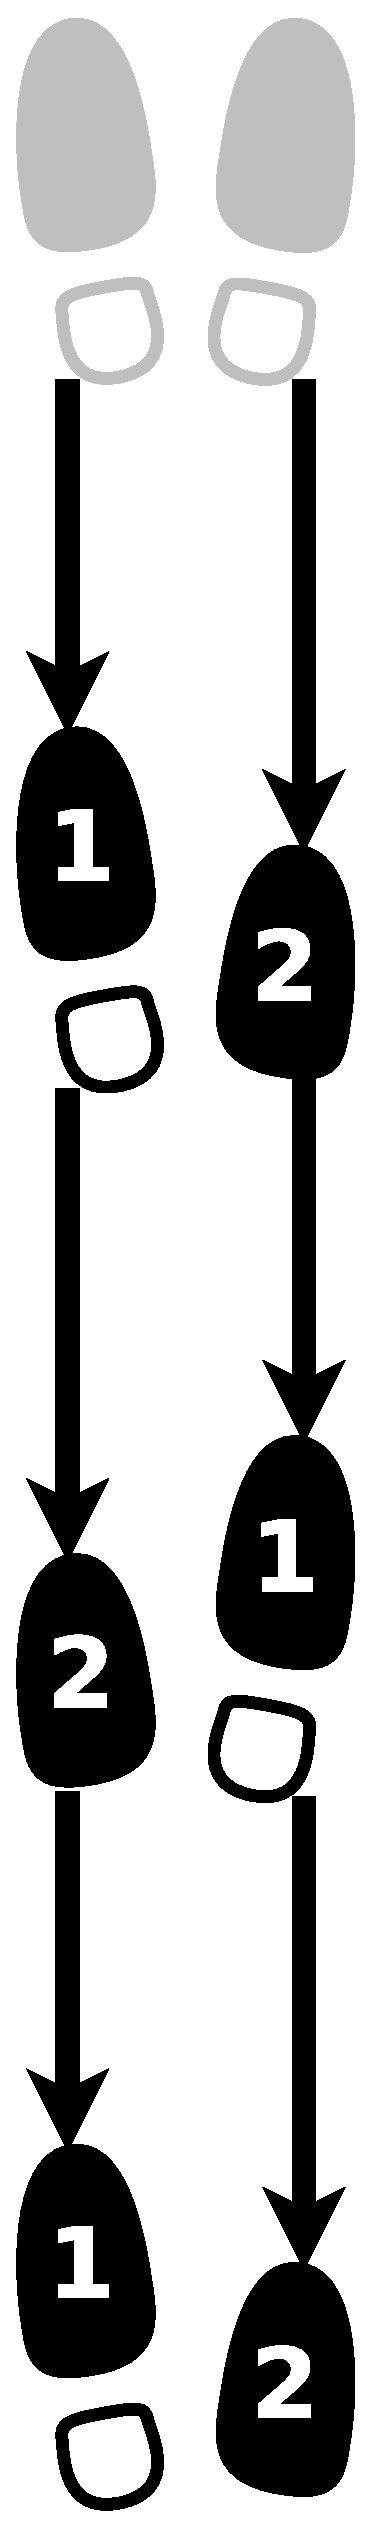
\includegraphics[width=0.25\textwidth]{chapters/cap-historia-sambagafieira/samba-cancao-basico-tras.eps}
        \caption{Passo básico para trás.}
        \label{fig:samba-cancao-basico-tras}
    \end{subfigure}
    \caption{Samba-canção da década de 1959.}\label{fig:samba-cancao-basico}
\end{figure}


\item \textbf{Samba-batucada},
\index{Dança!Samba-batucada} 

O samba-batucada é o samba de gafieira (primigênio) \cite[pp. 143]{perna2002samba}.

Existe uma menção sobre este estilo no ``Jornal do Brasil'', no dia 9 de janeiro de 1938,
onde se indica \cite[pp. 4]{musicasambavariasdef1}:
\begin{citando}%%
Tentativas isoladas de puro 
snobismo e ás vezes de compreensão 
inexata da origem da 
musica e dansa, chamam-no de samba jongo, \textbf{samba batucada} ou
pretendem mistura-lo com o fox, -- samba fox ou com a rumba samba-rumba.
\end{citando}



No livro ``Feitiço decente: Transformações do samba no Rio de Janeiro (1917-1933)'' (2001),
se comenta, sobre uma roda do samba, que para o dançarino solista  escolher a seu sucessor podiam
existir duas modalidades, em ``samba liso'' (com umbigada) ou em ``samba duro'' 
(ou batucada) no qual a umbigada é substituída por uma pernada \cite[pp. 109]{sandroni2001feitico}.
Deste comentário pode ser deduzido de onde vem a denominação \textbf{samba-batucada}, 
que surgiu nos salões de dança apos 1930; pois já existia uma tradição na nomenclatura,
em separar duas formas de dançar uma mais leve (a liso) e uma mais brusca (batucada);
assim, a variante de samba no salão que tendia a explorar movimentos muito  gingados, bruscos ou rápidos,
foi nomeado de samba-batucada, em contraposição ao samba liso onde né se flexionavam os joelhos pra dançar.  



O samba-batucada era, entre 1947 e 1959, uma dança com balanços que se dançava de joelhos flexionados  
e usava 3 movimentos por compasso, que exigia uma maior rapidez, 
especialmente no terceiro movimento que é mais rápido e curto \cite[pp. 61]{fornaciari1947aprender} \cite[pp. 58,66]{freitas1959danca};
seguindo essa descrição, 
o mais provável é que se dançara seguindo uma distribuição de tempos,
parecida ao ritmo do baião de 1949 \cite{CORTES2014}, como pode-se ver na Figura \ref{time:sambabatucada}.
\begin{figure}[H]
\centering
\begin{abc}[name=abc-sambabatucada]
X: 1 % start of header
K: C stafflines=1 % scale: C major
M: 2/4 %meter - compasso
%Q:1/4=100
V:1 clef=perc stem=up %name="TC"   sname="TC"
[V:1] |:  B3/2 B/2 B1 z1 | B3/2 B/2 B1 z1 | B3/2 B/2 B1 z1 | B3/2 B/2 B1 z1 :|
w:        P1   P2  P3      P1   P2  P3      P1   P2  P3      P1   P2  P3
\end{abc}
\caption{Frase de 8 tempos onde P1, P2 e P3 indicam o pé 1, 2 e 3 respetivamente.}
\label{time:sambabatucada}
\end{figure}

Sobre os passos usados na época, 
na Figura \ref{fig:samba-batucada-basico-frente} se mostra o passo básico para a frente do samba-batucada,
e na  Figura \ref{fig:samba-batucada-basico-tras} o mesmo movimento para trás;
em ambos casos se usa os 3 movimentos antes mencionados, e a cor cinza indica a posição inicial \cite[pp. 61-62]{fornaciari1947aprender} \cite[pp. 63]{freitas1959danca}. 
\begin{figure}[h]
    \centering
    \begin{subfigure}[b]{0.4\textwidth}
        \centering
        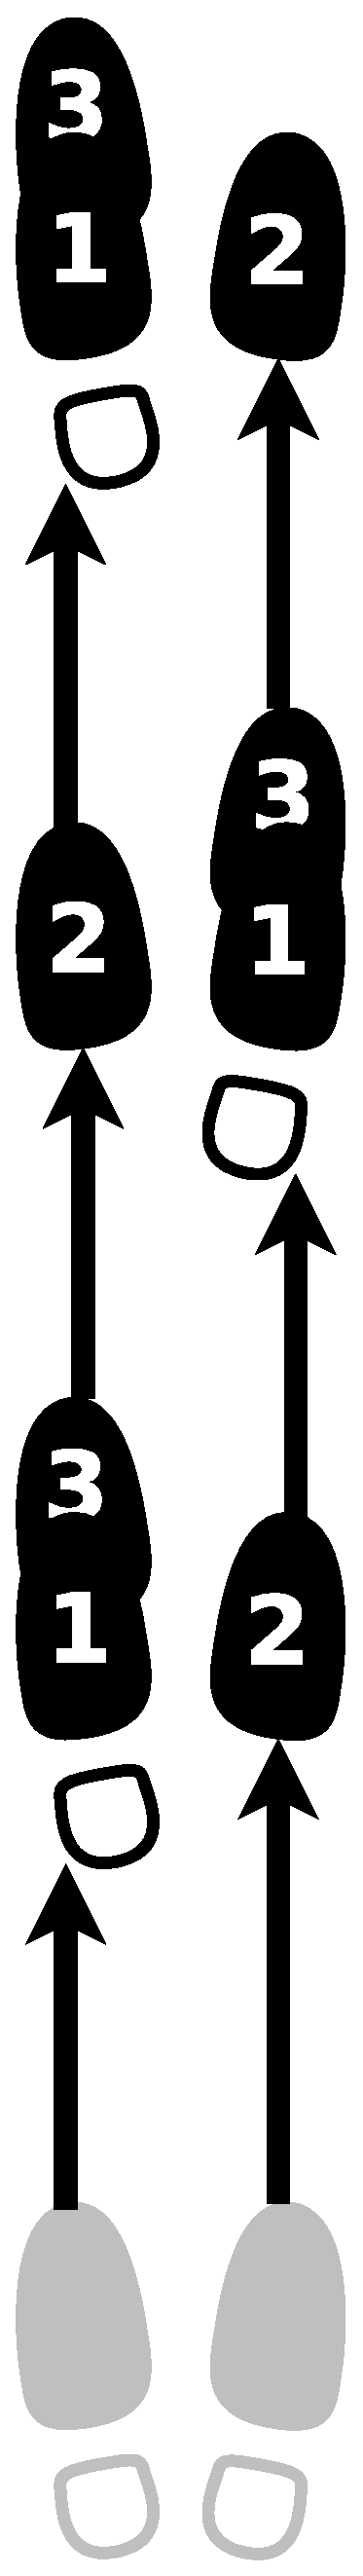
\includegraphics[width=0.25\textwidth]{chapters/cap-historia-sambagafieira/samba-batucada-basico-frente.eps}
        \caption{Passo básico para a frente.}
        \label{fig:samba-batucada-basico-frente}
    \end{subfigure}
    ~ %add desired spacing between images, e. g. ~, \quad, \qquad, \hfill etc. 
      %(or a blank line to force the subfigure onto a new line)
    \begin{subfigure}[b]{0.4\textwidth}
        \centering
	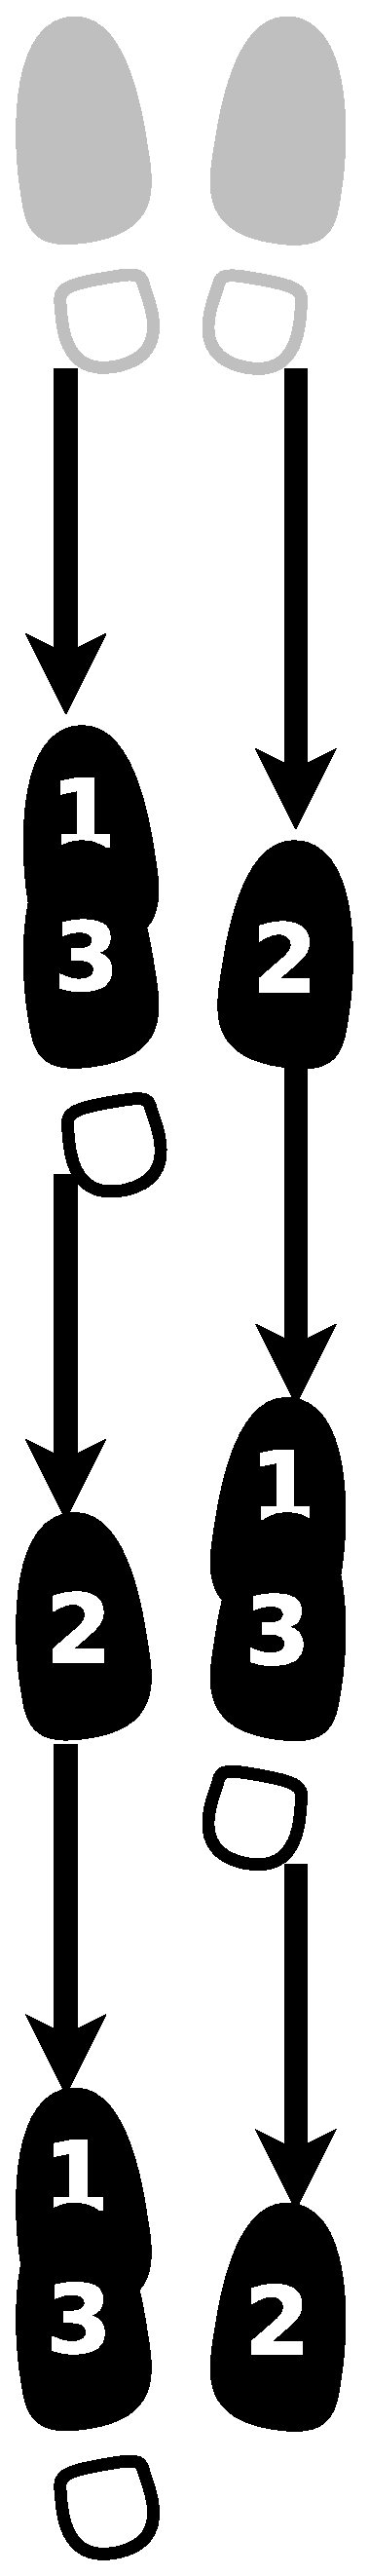
\includegraphics[width=0.25\textwidth]{chapters/cap-historia-sambagafieira/samba-batucada-basico-tras.eps}
        \caption{Passo básico para trás.}
        \label{fig:samba-batucada-basico-tras}
    \end{subfigure}
    \caption{Samba-batucada da década de 1959.}\label{fig:samba-batucada-basico}
\end{figure}

Outros passos conhecidos no ano de 1947, para este estilo de samba, tem nomes como: 
o pião, o balão, a cortada, a meia cortada, a joelhada, a patineta, e outros \cite[pp. 66]{fornaciari1947aprender};
porem, seguindo o Prof. Fornaciari, o pião e o balão são o mesmo movimento, 
sendo este o movimento mais importante do samba-batucada;
e a diferença do pião atual que se executa tradicionalmente em sentido horário,
o pião de 1947 se executava em sentido anti-horário \cite[pp. 68,72]{fornaciari1947aprender}.




\item \textbf{Samba liso}, 
\index{Dança!Samba liso}
Era uma dança com balanços que se dançava sem flexionar os joelhos;
este é um estilo de dança que perdura ainda ate nossos 
dias \cite[pp. 58,62]{freitas1959danca} \cite[pp. 143]{perna2002samba}, 
para mais detalhes ver a Seção \ref{subsec:estilosdedancapares}.
\end{itemize}

\subsection{Evolução do samba nos salões}

Com o passar dos anos foram agregados elementos de outras danças a esse primitivo, samba de gafieira;
por exemplo, movimentos do tango e do rock \cite[pp. 142]{perna2002samba}, 
obtendo assim a forma de dança que vemos hoje em dia, ver Figura \ref{fig:formuladosambagafieira2}.

Asim, podemos falar do samba de gafieira como dança, só apos da aparição do samba nos
salões de dança abertos ao público, e a partir da criação do termo gafieira pra definir a estes lugares.
Com a mistura destes dois acontecimentos obtemos o termo, samba de gafieira,
que iniciou seu caminho na dança, mas como uma descrição do âmbito da dança (e da música), que como nome próprio.
Porem, a formação dos movimentos e corporalidade desta dança tem um caminho que data desde muito tempo atrás,
desde os batuques, dos morros e das rodas.


A primeira referencia achada\footnote{Que não quer dizer a primeira existente.} 
na ``Hemeroteca Digital Brasileira'' da Fundação Biblioteca Nacional,
foi na ``Revista da Semana''(RJ), no dia 25 de dezembro de 1948,
onde na seção ``Eros Volusia'', subseção ``O pitoresco da excursão'', se indica \cite[pp. 48]{sambagafieirarefbn}
\begin{citando}
Ensinando o samba aos ministros da República, 
fazendo o povo vibrar com o \textbf{samba de gafieira}, entusiasmando
o meio intelectual com seu francês muito doce,
contando coisas desconhecidas aos dançarinos francêses,
fazendo a dança brasileira figurar nos Archives Internationales de la Danse.
Eros Volusia satisfez o grande ideal de sua vida artística, sentindo-se contente
com o que realizou na França, embora a Europa não dê dinheiro a ninguém.
O lucro artístico é que compensa.
\end{citando}


A Figura \ref{fig:sambagafieiracrono} mostra a cronologia do uso do termo samba de gafieira. 

\begin{figure}[h]
  \centering
    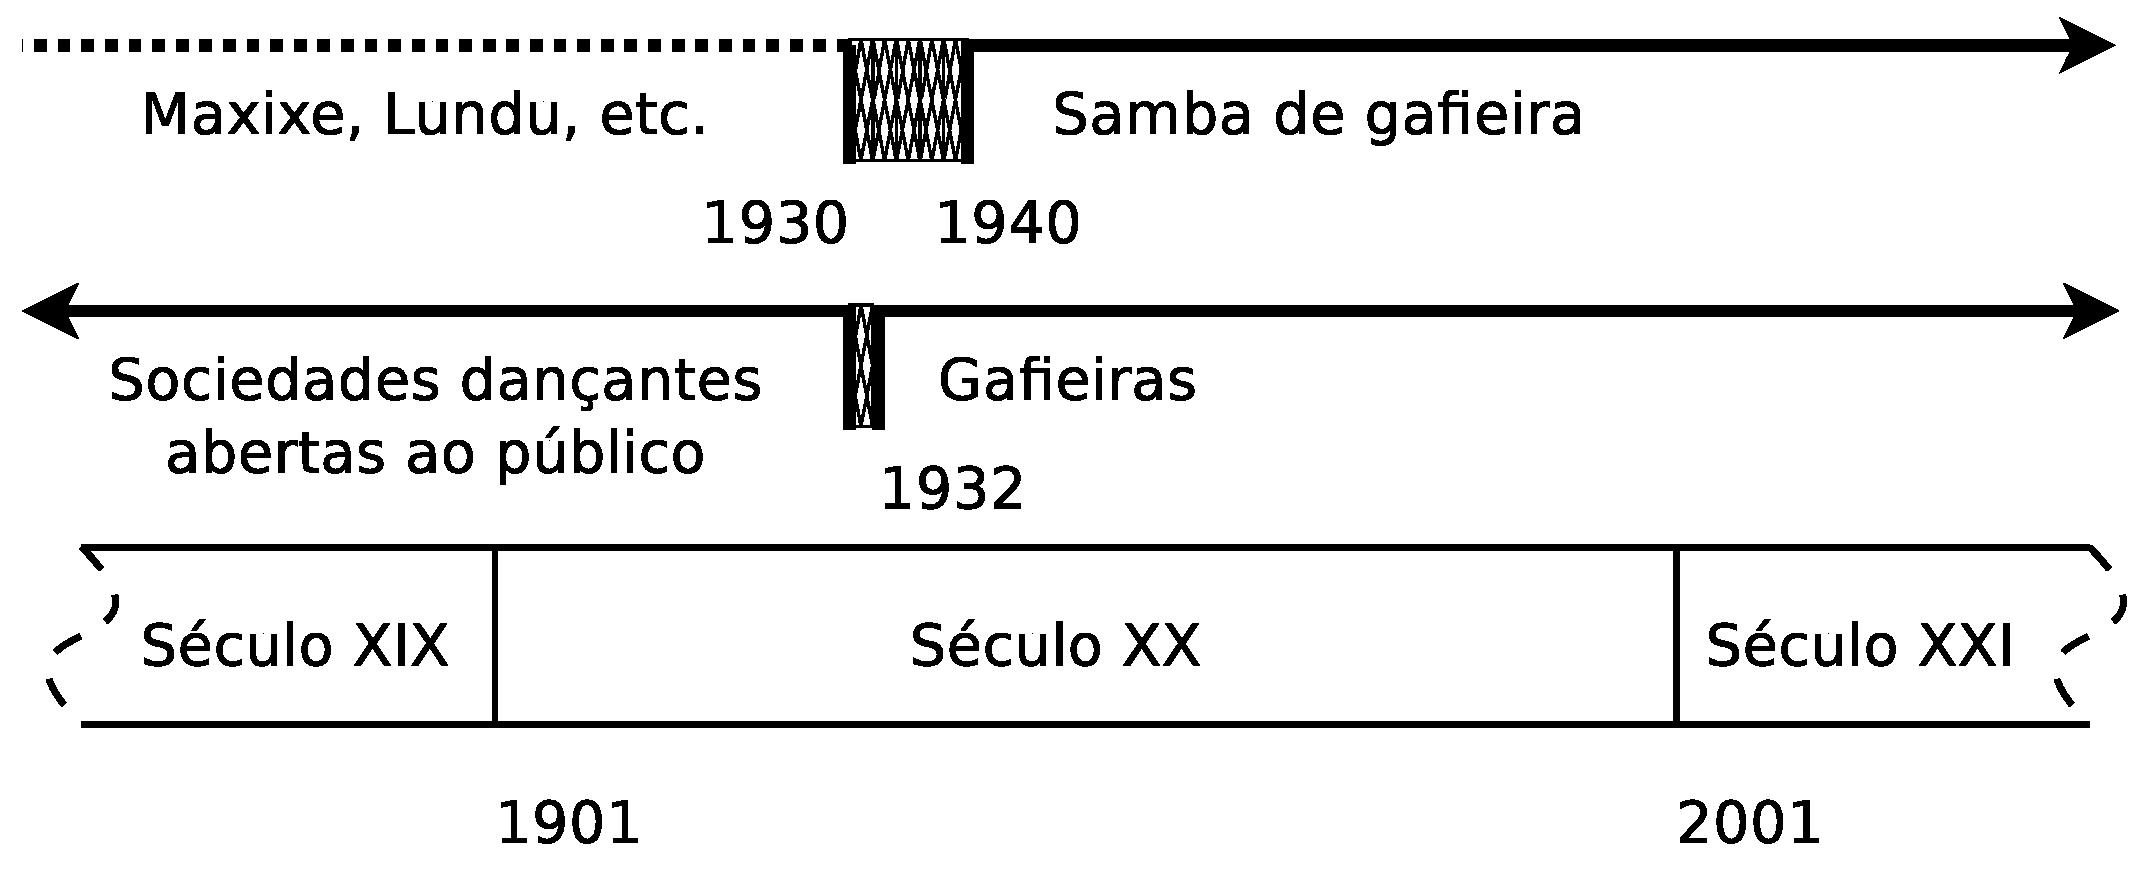
\includegraphics[width=1.0\textwidth]{chapters/cap-historia-sambagafieira/gafieira-crono.eps}
  \caption{ Cronologia da formação do samba de gafieira.}
\label{fig:sambagafieiracrono}
\end{figure}

%%%%%%%%%%%%%%%%%%%%%%%%%%%%%%%%%%%%%%%%%%%%%%%%%%%%%%%%%%%%%%%%%%%%%%%%%%%%%%%
%\clearpage
\section{Música para dançar samba de gafieira}
\label{subsec:gafieiradancaestilos}

Entre os estilos musicais em que o samba de gafieira (dança) se adapta bem, 
estão alguns dos subgêneros do samba; assim,
aqui mencionaremos uma lista de músicas que por sua graça, estilo e alegria,
a meu entender, podem ser dançados usando o samba de gafieira. Porem, 
estas músicas não pretendem ser máximos expoentes representativos, do subgênero em que estão agrupados;
e sim uma indicação ou orientação ao leitor, 
para treinar sua dança usando músicas em que possa ser mais confortável a experiencia.

\begin{itemize}
\item \textbf{Samba de gafieira (música)}
\begin{example} ~
\begin{itemize}
%\item ``Samba de padua'' interpretado pelo grupo Turma da Gafieira.
\item ``Samba de morro'' interpretado pelo grupo Turma da Gafieira.
%\item ``Piston da gafieira'' de Billy Blanco, interpretado por Jorge Beiga.
\item ``Piston da gafieira'' de Billy Blanco, interpretado por Zeca pagodinho \cite{barbosa2014zeca}.
\item ``Beija-me'' de Roberto Martins e Mário Rossi, interpretado por Zeca pagodinho \cite{barbosa2014zeca}.
\item ``Pisei num despacho'' de Geraldo Pereira e Elpídio Viana, interpretado por Zeca pagodinho \cite{barbosa2014zeca}.
%\item ``Tive sim'' de Cartola, interpretado por Zeca pagodinho \cite{barbosa2014zeca}.
%\item ``Tarzan, o filho do alfaiate'' de Noel Rosa e Vadico, interpretado por Zeca pagodinho \cite{barbosa2014zeca}.
%\item ``Se você visse'' de Dino 7 cordas e Del Loro, interpretado por Zeca pagodinho \cite{barbosa2014zeca}.
\end{itemize}
\end{example} 

\item \textbf{Samba de breque}
\begin{example} ~
\begin{itemize}
\item ``Baile no elite'' interpretado por Casuarina.
\item ``Eu sou a marrom'' interpretado por Alicione.
%\item ``Hoje sou diferente'' interpretado por Lenita Rodrigues.
\item ``Pra levantar poeira'' interpretado por Bodhar.
\end{itemize}
\end{example} 

\item \textbf{Pagode paulista (Sambalanço)}
\begin{example} ~
\begin{itemize}
\item ``Cheia de manias''  interpretado pelo grupo Raça Negra.
\end{itemize}
\end{example} 

\item \textbf{Partido alto}
\begin{example} ~
\begin{itemize}
%\item ``A língua'' interpretado por Beto lima.
\item ``Partido Alto'' interpretado por Aleh.
\end{itemize}
\end{example} 

\item \textbf{Pagode}
\begin{example} ~
\begin{itemize}
\item ``Trilha Do Amor''  interpretado pelo Grupo Revelação. 
\item ``A Batucada Te Pegou'' interpretado pelo Grupo Sou Muleke.
\item ``Dança da Solidão'' interpretado por Pagode de Mesa do álbum Terra Brasil. 
\item ``Eu e você sempre'' interpretado por Jorge Aragão
\end{itemize}
\end{example} 

\item \textbf{Samba-canção (música)}
\begin{example} ~
\begin{itemize}
\item ``Eu Quero E Sossego'' interpretado por Paulo Moura.
\item ``Só Louco'' interpretado por Luiz Melodia.
\item ``Você É a Fonte'' interpretado por  Quinteto em Branco e Preto.
\item ``Eu Quero é Sossego'' interpretado por Paulo Moura.
\end{itemize}
\end{example} 

\item \textbf{Bossa nova}
\begin{example} ~
\begin{itemize}
\item ``I Don't Know (Bossa Mix)'' interpretado por Erika do álbum ``I Don't Know''
\item ``Human Nature'' interpretado por Marcela Mangabeira.
\end{itemize}
\end{example} 


\item \textbf{Choro}
\begin{example} ~
\begin{itemize}
\item ``Choro de gafieira'' de Pixinguinha.
\item ``Chorinho de gafieira'' de Astor Silva.
\item ``Noites Cariocas'' de Jacob do Bandolim.
\end{itemize}
\end{example} 


\item \textbf{Samba-choro}
\begin{example} ~
\begin{itemize}
\item ``Escurinho'' interpretado por Corina Magalhães.
\item ``Tico Tico no Fubá'' interpretado por Leci Brandão.
\end{itemize}
\end{example}

\end{itemize}

A Figura \ref{fig:gafieiradancaestilos} mostra um resumo de alguns dos 
subgêneros do samba onde pode ser dançado o samba de gafieira.
\begin{figure}[h]
  \centering
    \includegraphics[width=0.7\textwidth]{chapters/cap-historia-sambagafieira/gafieiravcmusica.eps}
  \caption{ Subgêneros do samba onde pode-se dançar samba de gafieira.}
\label{fig:gafieiradancaestilos}
\end{figure}


%\chapterimage{chapter_head_2.pdf} % Chapter heading image

\chapter{Historia do samba e da dança}

%%%%%%%%%%%%%%%%%%%%%%%%%%%%%%%%%%%%%%%%%%%%%%%%%%%%%%%%%%%%%%%%%%%%%%%%%%%%%%%%
%% SECTION
%%%%%%%%%%%%%%%%%%%%%%%%%%%%%%%%%%%%%%%%%%%%%%%%%%%%%%%%%%%%%%%%%%%%%%%%%%%%%%%%
\section{\textcolor{green}{Historia do samba}}\index{Historia do samba}
O samba como principal manifestação da cultura brasileira está bem reconhecida no Brasil do seculo XXI;
porem, o caminho da palavra samba, ou da ideia do samba, inicia muito tempo atrás;
pois como mostraremos mais adiante, existiu uma transição entre os termos ``batuque'' e ``samba''.
Nos inícios do seculo XIX
se designava com a palavra ``batuque''  a qualquer reunião de ``pretos'' (em expressões próprias da época) realizando danças entendidas como africanas\footnote{
Porem no Brasil existem registros desta palavra desde o século XVIII \cite[pp. 85]{sandroni2001feitico}. }
\cite[pp. 54]{de4danccas} \cite[pp. 73]{lara2007memoria}.
Um exemplo disto pode ser visto numa carta ao redator do ``Correio Braziliense''  (Londres, ING),
sobre os negócios públicos em Pernambuco,
escrita o dia 3 de dezembro do 1816, e publicada em 1817 \cite[pp. 468]{batuqueBraziliense},
onde se menciona\footnote{\label{footort}A forma da escrita corresponde ao texto original}:
\begin{citando}%%
Quasi dous annos depois, o Ouvidor das Alagoas, que não tinha tido parte neste Drama,
sonhou com outro levante de pretos na sua comarca, 
fundamentado unicamente em um \textbf{batuque} de dança, 
que alguns faziam nas inmmediaçoens de um Engenho de assucar, ...
\end{citando} 
Pelo que se observa, 
a palavra ``batuque'' não se usava para referenciar a uma dança em particular e sim aos festejos dos negros em geral \cite[pp. 85]{sandroni2001feitico}.

\PRLsep{*}

Paralelamente na historia, a palavra samba estava iniciando a ser usada como parte
das expressões nestos festejos populares. 
Isto pode ser visto na ordem do dia do Quartel do Governo das Armas em
Pernambuco, 8 de julho de 1830, publicado no jornal ``Diario de Pernambuco''(PE), 
onde se  relata\footref{footort} \cite[pp. 3]{sambadiariodepernanbuco}:
\begin{citando}%%
Naõ existindo fora da Capital nos diferentes pontos,
onde se achão destacadas as Companhias deste Corpo, 
hum serviço ativo, a que sejão ellas forçadas, 
necessariamente a occiozidade dispora' 
aos mais bem conduzidos a se entreterem nas pescarias de curraes e trapaçoens de coqueiros,
em cujos passatempos sera' recebida com agrado a viola, e o \textbf{samba};
e aos peraltas, cada vez os fara' mais dezenvolvidos na conjugação do verbo surripio.
\end{citando}
Anos posteriores podemos encontrar uma dualidade no uso da palavra samba, 
tanto no sentido de música como de dança; por exemplo, no jornal ``O Capuceiro''(PE),
do dia 3 de fevereiro de 1838, temos uma referencia ao samba como música,
onde ademais se ressalta a beleza da interpretação musical;
o seguinte é um fragmento desse texto\footnote{\label{footort2}A forma da escrita corresponde ao texto original} \cite[pp. 1]{sambaperiodicoocapuceiro}:
\begin{citando}%%
Segue se, que tão perfeita na Cantoria era Catalini, ou a Pasta,
como pai Antonio descantando no seu birimbau; que tanto val huma garatuja da China,
que vinhão nos bules, e bandejas,
como as pinturas de Rafael, de Rubens, ou do Corregio;
que tão agradavel he hum \textbf{samba} d'almocreves, como a Semiramis,
a Gaza-ladra, o Tencredi, \&c. de Rossini, ...
\end{citando}
Também podemos achar outra referencia do samba no sentido musical, no jornal ``Diário do Rio de Janeiro''(RJ),
do dia 19 de abril de 1939, onde se menciona\footref{footort2} \cite[pp. 1]{sambadiariorj1}:
\begin{citando}%%
Em quanto o cortezão, o palaciano, o gamenho, o literato, o magistrado etc., 
espancão melanconias, desvanecem cuidados tomando em ricas bocetas o cheiroso rapé;
o laborioso maluto, a quem furtárão o cavalinho (que é a menina dos seos olhos)
depois de affligir-se, e praguejar em balde arranca do quijeje (bolso na celoura)
o encebado cornimboque, saca lhe com estalo e tapadoura, e chafurdando as ventas em duas,
ou trez pitadas mestras da sua torradinha, esquece-se do cavallo, resigna-se com sua sorte,
e com uma viola nas unhas zangarrêa o \textbf{samba} por uma noite inteira.
\end{citando}
Por outro lado, temos uma referencia ao samba relacionando-o com a dança, no jornal ``O Capuceiro''(PE),
do dia 12 de novembro de 1842\footnote{Só 6 anos apos referenciar o samba como música, 
no mesmo jornal, é usado o mesmo termo agora relacionado com a dança.}, 
onde mencionam\footref{footort2} \cite[pp. 5]{sambaperiodicoocapuceiro2}:
\begin{citando}%%
Aqui pelo nosso mato,\\
Qn'stava então mui tatamba,\\
Não se sabia outra cousa,\\
Senão a \textbf{dansa do samba}.
\end{citando}
Neste ultimo texto vemos que ainda se diz a \textbf{dança do samba} e não dançar o samba,
mas é possível observar como o termo vai se fusionando com a dança.
Seguindo esta linha de pensamento, 
podemos ver outro exemplo no Jornal ``O Guaycuru''(BA), do dia 26 de maio de 1846,
onde podemos ler o seguinte texto\footref{footort2} \cite[pp. 2]{sambaperiodicooguaycuru}:
\begin{citando}%%
Todavia o famigerado Salles, sem respeito algum aos institutos de sua ordem, 
foi-se pòr na Cachoeira a divertir talvez \textbf{dançando o samba}...
Que bello exemplar da vida religiosa!?
\end{citando}
Como tem sido visto, 
para esta data já se podia ver como as pessoas entendiam o samba como uma dança.
Porem, não terá que se esperar muito pra achar referencias mostrando ao samba
como uma expressão cultural em si mesma, 
uma declaração deste tipo pode ser achada no jornal ``O Cosmorama na Bahia'' (BA), 
no dia 15 de dezembro de 1849, onde menciona\footref{footort2} \cite[pp. 2]{sambaperiodicoocosmorama}:
\begin{citando}%%
Cousa já muito antiga para engordar os patinhos. 
Para o espectaculo seguinte haverá um \textbf{SAMBA} á moda da Bahia, 
em que entram os negreiros todos.
\end{citando}

\PRLsep{*}
Retomando o tema do batuque

\PRLsep{*}


Assim, como mostrado anteriormente e resumindo as ideias, 
na literatura do Brasil já temos referencias da palavra ``samba'' desde o ano de 1830; 
porem como menciona Sandroni C. no seu livro ``Feitiço decente: transformações do samba no Rio de Janeiro'', 
falando especificamente do Rio de Janeiro, 
a palavra samba foi pouco conhecida ate o último quartel do século XIX \cite[pp. 86]{sandroni2001feitico};
este dado cobrará importância quando o termo seja relacionado com as gafieiras.
Por outro lado, a palavra  ``batuque'' usada para designar festejos populares com danças, foi muito recorrente ate inícios do seculo XX, 
onde a palavra ``samba'' virou mais popular para descrever estas atividades \cite[pp. 85]{sandroni2001feitico} \cite[pp. 47]{diniz2008almanaque}; 
a Figura \ref{fig:sambacrono} descreve o uso destas palavras ao longo do tempo.
\begin{figure}[h]
  \centering
    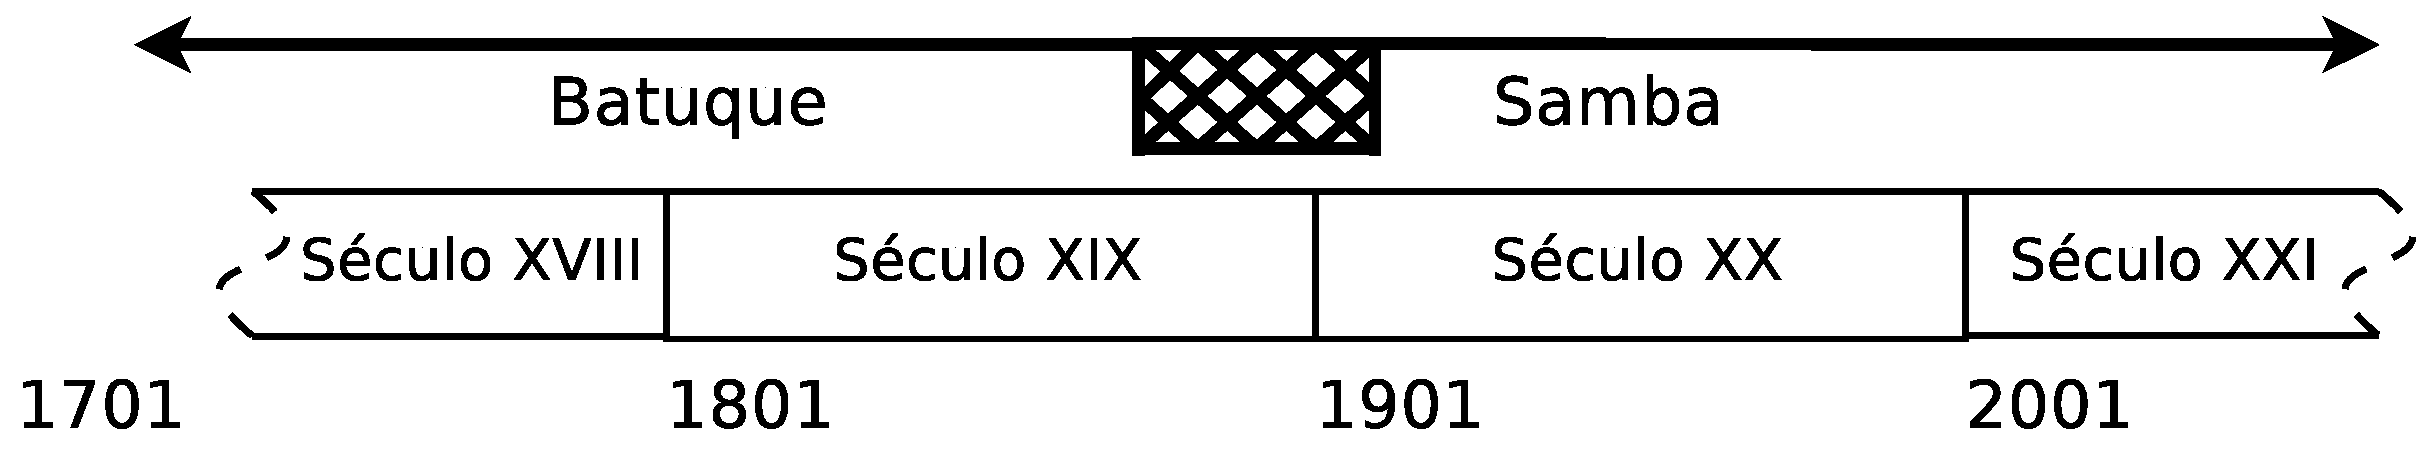
\includegraphics[width=0.85\textwidth]{chapters/cap-historia/samba-crono.eps}
  \caption{Cronologia da designação geral dos festejos de pessoas, de raça negra, no Brasil.}
  \label{fig:sambacrono}
\end{figure}


Entre as explicações da origem da palavra ``samba'', 
a mais conhecida, é a que promove que esta vem do idioma quimbundo, 
sendo derivado da palavra ``semba''  que significa umbigada \cite[pp. 47]{diniz2008almanaque} \cite[pp. 50]{da2015historia}.
Uma referencia muito conhecida deste vinculo é a descrita no livro ``O negro e o garimpo em Minas Gerais''
de Mata Machado Filho, onde ele comenta que ``os negros corrigem para semba se 
alguém lhes fala em samba'' \cite[pp. 85]{sandroni2001feitico}. Assim se vê que existe
desde antanho uma relação entre as palavras, 
samba, semba e umbigada.

\begin{comment}
Entre as danças "profanas" \cite[pp. 85]{sandroni2001feitico} afro-brasileiras o gesto da umbigada é um elemento muito caraterístico,
de modo que em 1961 Edson Carneiro definiu e englobou as danças que realizam este 
gesto como ``samba-de-umbigada'' . Assim tradições 
musicais como o samba de roda, o jongo, o lundu, o coco, o calango e o cateretê, 
seguindo Edson são englobadas com  ``samba-de-umbigada'' \cite[pp. 85]{sandroni2001feitico}.
\end{comment}


%%%%%%%%%%%%%%%%%%%%%%%%%%%%%%%%%%%%%%%%%%%%%%%%%%%%%%%%%%%%%%%%%%%%%%%%%%%%%%%%
%% Capitulo
%%%%%%%%%%%%%%%%%%%%%%%%%%%%%%%%%%%%%%%%%%%%%%%%%%%%%%%%%%%%%%%%%%%%%%%%%%%%%%%%
\chapterimage{chapter_head_2.pdf} % Chapter heading image

\chapter{Historia das gafieiras}
\index{Historia das gafieiras}

%%%%%%%%%%%%%%%%%%%%%%%%%%%%%%%%%%%%%%%%%%%%%%%%%%%%%%%%%%%%%%%%%%%%%%%%%%%%%%%%
\section{Gafieira}
\label{def:Gafieira}
\index{Gafieira}
Atualmente o termo gafieira indica um baile de clube particular, com entrada paga e frequência livre. 

\begin{itemize}
\item \textbf{1979 em adiante:} Se entende que as gafieiras são locais de lazer 
e dança onde existe bom comportamento e muita compostura,
em perfeita integração racial; de modo que, 
a gafieira é sinônimo de baile em salão espaçoso como boa música orquestral \cite[pp. 10-11]{respeitojournalbrasil1}.

\item \textbf{1932 ate antes de 1979:} O termo gafieira foi associado a lugares de baixa ralé, onde 
se aconteciam frequentemente delitos e trágicos acontecimentos \cite[pp. 11]{gafieirajournalbrasil1} \cite[pp. 12]{gafieirajournaloradical1} \cite[pp. 10-11]{respeitojournalbrasil1}.

\item \textbf{1932:} popularização do termo gafieira, apos o
incidente entre o jornalista Romeu Arêde (Picareta) e o empresario e fiscal de salão Júlio Simões,
que provocou que  Picareta publica-se uma matéria apontando 
ao clube de Júlio como uma gafieira \cite[pp. 3 - cad. 3]{juliosimoes} 
\cite[pp. 21]{efege1974maxixe} \cite[pp. 78]{coutinho2006cronistas};
pelo que este último decidiu apelidar seu exitoso ``Elite clube'' como gafieira;
espalhando-se rapidamente esta denominação a outros clubes similares. 
Assim, o termo queda vinculado a clubes de dança da classe média,
onde eram aceitos todas as pessoas sem nenhum tipo de preconceito racial, 
prévio pago da entrada \cite[pp. 6 - cad. B]{entrevistajuliojournalbrasil1}.


\item \textbf{1917 ate 1932:} 
Inícios do uso do termo gafieira, indicando bailes populares \cite[pp. 29]{instituto1987revista} de entrada paga
ou bailes criados por motivo do carnaval; sendo que, as referencias bibliográficas
achadas são nas semanas próximas ao carnaval \cite[pp. 4]{oldgafieira1} 
\cite[pp. 7]{oldgafieira2} \cite[pp. 4]{oldgafieira3} \cite[pp. 5]{oldgafieira4},
o que mostra a notoriedade que adquiriam esses eventos, ou locais, nessas datas.
\end{itemize}

%%%%%%%%%%%%%%%%%%%%%%%%%%%%%%%%%%%%%%%%%%%%%%%%%%%%%%%%%%%%%%%%%%%%%%%%%%%%%%%%
\section{Cronologia das gafieiras}


%%%%%%%%%%%%%%%%%%%%%%%%%%%%%%%%%%%%
%\PRLsep{Bailes na década de 1800}

Seguindo o jornalista Agostinho Seixas,
entre os anos de 1847 e 1848, na Cidade Velha, no Rio de Janeiro,
já existiam  bailes e clubes recreativos, 
que hoje denominaríamos como \textbf{gafieiras} \cite[pp. 11]{respeitojournalbrasil1}.
Seixas achou como primeira referencia na suas pesquisas, que entre essas datas,
Dona Francisca Pacheco da Silva, fazia um requerimento 
à ``Excelentíssima Câmara'' (que foi concedido) para a autorização 
da sua sala de bailes, na Rua da Alfândega, 327 \cite[pp. 11]{respeitojournalbrasil1} \cite[pp. 71]{perna2002samba};
este requerimento foi catalogado como sala de danças, 
com a característica de ter entrada paga.
Seguindo o fiscal que acompanhava o requerimento,
ele não achava artigo que regulamentasse esse tipo de local 
de diversão ou dança; lembremos que nessa época
o padrão era ter clubes fechados que tinham um determinado número de sócios \cite[pp. 11,12]{respeitojournalbrasil1}.



%%%%%%%%%%%%%%%%%%%%%%%%%%%%%%%%%%%%
\PRLsep{Bailes na década de 1900}


Para inícios do século XX, podiam ser achadas varias associações para negros e mestiços, 
com distintas  finalidades, como: sociedades beneficentes, literárias, dramáticas, esportivas 
e as ``sociedades dançantes e recreativas'' abertas a um público geral
\cite[pp. 154-155]{neres1999negro} \cite[pp. 71]{de2008bexiga}.
Estas associações geralmente não tinham local próprio, 
e tinham que alugar espaços que terminavam sendo salões de velhos sobrados
ou similares \cite[pp. 154-155]{neres1999negro} \cite[pp. 49]{diniz2003almanaque}.
Entre as organizações sociais recreativas mais comuns da época tínhamos, 
os cordões\footnote{Os cordões eram grupos festivos de dança e música, 
com pessoas mascaradas com figurinos de reis, de
bichos, de pajens, de guarda, etc., tocando instrumentos africanos \cite[pp. 23-24]{fernandes2001escolas}},
os ranchos\footnote{Quando os cordões desapareceram estes se transformam em ranchos (depois de 1908), 
agregaram instrumentos de corda e metais, e inciou a ser tocado a marcha-rancho,
os ranchos eram cordoes mais civilizados \cite[pp. 24]{fernandes2001escolas}} 
e os zé-pereiras\footnote{ Uma sociedade recreativa do ``Ze-pereira''
é uma sociedade dedicada a dança carnavalesca \cite[pp. 10]{simoesjournalbrasil1}} 
\cite[pp. 10]{simoesjournalbrasil1}.


Uma destas sociedades de dança do inícios do seculo XX, que agora definiríamos como gafieira, 
foi a ``Sociedade de Danças Clovis Invencivel''\footnote{Em algumas versões 
``Clovis Invencivel'' é referenciado como ``Clowns Invencíveis'' \cite[pp. 3 - cad. 3]{juliosimoes} ou 
``Clovis Invencíveis'' \cite[pp. 10]{simoesjournalbrasil1}}, 
esta foi fundada no Rio de Janeiro em 1906, 
na qual eram populares concursos de valsa, polca ou quadrilha \cite[pp. 6 - cad. B]{entrevistajuliojournalbrasil1}.
O dono da ideia da criação destes concursos foi um muito jovem e fiscal do salão, Júlio Simões,
que a seus 16 anos pensou numa sociedade de dança diferente dos da época,
que se dedicavam a ``bater bumbo'' (bailes carnavalescos ou de zé-pereira), 
a uma dedicada a ``arrasta-pés'' (bailes de salão) 
\cite[pp. 6 - cad. B]{entrevistajuliojournalbrasil1} \cite[pp. 3 - cad. 3]{juliosimoes} \cite[pp. 10]{simoesjournalbrasil1}.

Com o surgir dos lugares de baile, em 1915 \cite[pp. 1 - cad. B]{gafieira2000reis},  
Júlio Simões, foi chamado pelos sócios\footnote{Os 
sócios fundadores da ``Kanaga do Japão'' são José Constantino da Silva 
e José de Paiva Brito \cite[pp. 1 - cad. B]{gafieira2000reis}} da ``Kanaga do Japão'' para dirigir seu novo clube,
lugar de grande tradição no Rio de Janeiro, e muito popular na época,
no qual o conjunto encarregado de animar o local era chefado por Sinhô e Bulhões de Carvalho,
que receberam o título popular de ``reis da valsa'',
com torneios de dança que duravam ate 55 
minutos dançando uma valsa rápida \cite[pp. 3 - cad. 3]{juliosimoes} \cite[pp. 1 - cad. B]{gafieira2000reis} \cite[pp. 6 - cad. B]{entrevistajuliojournalbrasil1}.
Nas festas comandadas por Júlio, era comum ver dançar samba, polca, 
valsa e quadrilha, que ele mesmo marcava no salão \cite[pp. 1 - cad. B]{gafieira2000reis}. 


Para o ano 1930, estas sociedades dançantes tinham ganhado muita popularidade. 
Assim, apos a morte de um socio e o fechamento da ``Kananga do Japão'' 
em 1929 \cite[pp. 3 - cad. 3]{juliosimoes}  \cite[pp. 11]{eliteinaugura} \cite[pp. 1 - cad. B]{gafieira2000reis}, 
Júlio Simões procura a Heitor Persegani e  Hilário Jovino, 
e decidem fundar o local de danças chamado ``Elite club'' \cite[pp. 11]{eliteinaugura} \cite[pp. 13]{respeitojournalbrasil1},
agora chamado ``Elite clube'' \cite[pp. 3 - cad. 3]{juliosimoes},
na Rua Frei Caneca n. 4 - Centro, Rio de Janeiro - RJ;
sendo o 17 de julho de 1930 seu baile inaugural 
\cite[pp. 11]{eliteinaugura} \cite[pp. 3 - cad. 3]{juliosimoes} \cite[pp. 10]{simoesjournalbrasil1}.

Uma descrição de uma destas sociedades dançantes, anterior a 1931, pode ser vista no livro "O cabrocha"; 
escrita  por Jota Efegê em 1931; 
sobre a ``Sociedade Recreativa Familiar Bohemios de Botafogo'' \cite[pp. 24-26]{jotaefege},
a continuação é mostrado um extracto desse texto:
\begin{citando}%%
O salão, comquanto não fosse de grandes dimensões, era
de um tamanho regular, confinando com uma pequena saleta
onde tambem se dansava; estava bem affluido. Numa
heterogeneidade foliã, via-se desde a crioulinha blasée, sem
elegancia, desalinhada, á mulatinha pernostica de faces
avermelhadas por um carmin berrante, cabello engommado e
subjugado por travessas e grampos, num á la garçonne
forçado, mas exigido pela moda. Em meio dessas "cabrochas"
e "roxinhas", viam-se algumas moças brancas de apparencia
sobria. São as meninas que não podem fazer um vestido de
seda ou calçar sapatos de setim, para se apresentarem no
Fluminense ou no Flamengo e que nestes clubes se divertem,
ficando em evidencia por serem brancas.  %~\\
(Jota Efegê)
\end{citando}

%%%%%%%%%%%%%%%%%%%%%%%%%%%%%%%%%%%%
\PRLsep{Inícios do uso do termo gafieira}

Fazendo uma pesquisa na ``Biblioteca Digital da Fundação Biblioteca Nacional''
podemos achar referencias ao termo \textbf{gafieira} desde 1917\footnote{Mesmo 
ano em que foi lançado o samba ``Pelo telefone'', sendo um exito total no carnaval desse ano.}.


A primeira referencia pode ser vista no jornal ``O Imparcial'' (RJ),
do dia 17 de janeiro de 1917, como o título ``Batalha de confetti'',
no qual se anuncia que na rua Guimarães se terá uma grandiosa batalha,
organizada pelo ``bloco dos pesados'', conformado por \cite[pp. 4]{oldgafieira1} \cite[pp. 629]{spielmann2016reflexoes}:
\begin{citando}
Lourenço dos Santos (Lord Sorvete),\\
Antonio dos Santos (Lord Massa),\\
Antonio Lima (Lord Repinica),\\
Raul Dantas (Lord Ronqueira),\\
Almeidinha (Lord Prrrrr...!),\\
Arlindo dos Santos (\textbf{Lord Gafieira}),\\
Joaquim Mello (Lord Frango d'Agua),\\
Juvenal Branco (Lord Pé Pequeno),\\
Eudoxio dos Santos (Lord Garganta) e\\
Jorge Vença (Lord Come Bola).
\end{citando}
Pelo contexto do anuncio, e pela semelhança com os outros apelidos, 
pode-se perceber que o termo \textbf{gafieira} tem um significado alegre,
cotidiano ou extravagante, mas é difícil extrair alguma outra conclusão.

A seguinte referencia aparece um ano depois, no mesmo jornal,
no dia 8 de fevereiro de 1918, como o título ``Grande batalha de confetti'',
na qual se anuncia que a batalha é organizada pelo ``bloco da rapaziada'',
do ``\textbf{Club da Gafieira}'', a qual também terá a participação 
da \textbf{orquestra do ``Gafieira''} que tocará adoráveis tangos;
e se finaliza falando que  \cite[pp. 7]{oldgafieira2} \cite[pp. 629]{spielmann2016reflexoes}:
\begin{citando}
Serão distribuídos brindes áquelles que mais se têm distinguido nos bailes do valoroso ``\textbf{Gafieira}''.
\end{citando}
Nesta referencia, já podemos observar que a palavra gafieira é relativa à celebrações do carnaval, 
e a lugares ou eventos de bailes,
nos quais, por exemplo, se dançam tangos; 
pelo que a palavra \textbf{gafieira} é usada no nome da orquestra,
e no apelido de um integrante, o valoroso \textbf{Gafieira}.

Um ano depois na ``Gazeta de Noticias'' (RJ),
no dia 3 de março de 1919, com o título ``Club dos carnavalescos do Andarahy'' e subtitulo ``1ra Critica - A Gafieira'',
se anuncia que a ``Banda de clarins'' e a ``Banda de música'',
tocarão uma espirituosa ``charge'' aos bailes de clubs de mil réis por cabeça, 
na qual era  usada a seguinte letra \cite[pp. 5]{oldgafieira3} \cite[pp. 629]{spielmann2016reflexoes}:
\begin{citando}
Cinco tostão vale a varsa!\\
Grita o fiscal do salão:\\
Tirem as dama depressa,\\
Não perquem a casião!\\ ~\\
Sapeca o piston com força,\\
Requebra mais, já se vê!\\
Que depois da contradança,\\
A dama vai p'r'o bufê.\\ ~\\
Paga a entrada e não estrilla!!\\
Que isto aqui é uma deliça!\\
Se porte bem, seu varsista!\\
Cuidadinho e'n a poliça!...
\end{citando}
Nesta última referencia já podemos ver claramente o sentido do termo gafieira,
identificando a um lugar de dança, em especifico a esses lugares com entrada paga a mil réis por cabeça.
Para ter uma ideia de se este preço é pouco ou muito, podemos compará-lo com o 
preço do jornal em que foi publicado o texto, sendo este de 100 RS \cite[pp. 1]{oldgafieira3};
ou também por essas épocas, 
quando a entrada custava 2 mil réis o preço de uma cerveja  era  de 800 réis \cite[pp. 1 - cad. B]{gafieira2000reis}.
Outro dado interessante é o uso do termo ``fiscal de salão'', 
figura de autoridade que já estava presente 
nas sociedades dançantes do seculo XX, como por exemplo na 
``Sociedade de Danças Clovis Invencivel'' em 1906, pelo que queda claro
a que lugares se refere o termo gafieira.


Podemos ver outra noticia relativa as gafieiras, no dia 19 de janeiro de 1920, 
no jornal ``A Razão'' (RJ), no qual se
publica uma reportagem com o título 
``Charivari num club suburbano - Fechado pela policia'',
se referindo ao clube ``Fenianos de Cascadura'',
que seguindo o descrito, este clube era 
ponto de reunião de gente desclassificada, 
que realizava seus bailes os sábados e domingos,
cobrando na entrada $1\$100$ por cabeça.
O seguinte texto é uma porção daquela reportagem \cite[pp. 4]{oldgafieira4} \cite[pp. 629]{spielmann2016reflexoes}:
\begin{citando}
A policia local, que é a do $20^o$ districto,
já estava farta do trabalho que o club 
constantemente lhe dava e de receber reclamações 
dos moradores visinhos.\\
Deliberou então o delegado, dr. Coelho
Gomes, fechar o club, mais conhecido por 
``\textbf{Gafieira}'', na primeira occasião que `e apresentasse.\\
Ante-hontem, sabbado, á noite, o club 
deu o acostumado ``baile'' e ás 5 horas da 
madrugada houve, ali um ``charivari'' medonho,
que poz o largo de cascadura em polvorosa. 
\end{citando}
O termo charivari se usa para indicar música discordante, 
confusão, motim, tumulto, barafunda \cite[pp. 53]{almeida1996dicionario}, etc.
Assim, podemos ver como o termo gafieira, 
estava relacionado a clubes de dança com entrada paga,
e que era frequentado por pessoas de poucos recursos econômicos. 
Também é interessante ressaltar que as referencias achadas correspondem,
a datas próximas ao carnaval, o que mostra o vinculo ou o maior interesse 
destes locais nestas datas. 

Ainda podem ser achadas outras referencias ao termo \textbf{gafieira} na década de 1920,
nelas podemos destacar apelidos usados por professores de dança,
ou referencias de musicas com letras indicando que gafieiras 
são frequentadas por crioulas e/ou criadas.


%%%%%%%%%%%%%%%%%%%%%%%%%%%%%%%%%%%%
\PRLsep{Popularização do termo gafieira}

Seguindo o jornalista e cronista, Jota Efegê, %%Júlio Simões e o historiador,
o termo ``gafieira'' foi criado pelo cronista carnavalesco, 
Romeu Arêde\footnote{Em algumas versões está  referenciado como Romeu Aredo \cite[pp. 188]{raca1999}.}, 
também conhecido como ``Picareta'' \cite[pp. 29]{instituto1987revista}\cite[pp. 3 - cad. 3]{juliosimoes} 
\cite[pp. 21]{efege1974maxixe} \cite[pp. 78]{coutinho2006cronistas}, 
colunista da seção recreativa do ``Jornal do Brasil'' desde 1930 ate 1941
e anteriormente do vespertino ``Vanguarda'' (1922-1930) \cite[pp. 58-59]{efege1982figuras} 
\cite[pp. 6 - cad. B]{entrevistajuliojournalbrasil1};
porém não é indicada, por Jota Efegê, referencia nenhuma sobre a data de criação.
Efegê indica que o termo ``gafieira'', possivelmente deriva de 
``cabroeira''\footnote{Cabroeira: Malta de indivíduos chamados cabras, 
de capangas assalariados para assassinar ou para fazer o mal \cite{diciocabroeira}.} 
ou ``gaforinha'' \cite[pp. 3 - cad. 3]{juliosimoes}.
Por outro lado, Júlio Simões, socio e administrador do ``'Elite club', 
afirma\footnote{Seguindo a ``Revista do Instituto Histórico e Geográfico do Rio de Janeiro'' (1987),
Jota Efegê afirma que foi Romeu Arêde quem atrelou o termo gafieira aos clubes de dança no incidente no ``Elite clube''.} 
que o jornalista Romeu Arêde tinha a costume de entrar, 
comer, beber, dançar e não pagar \cite[pp.13 ]{respeitojournalbrasil1},
e que quando ele impediu ao boêmio jornalista e seus acompanhantes (5 ou 6) o ingresso no ``Elite'', 
porque a entender de Júlio o jornalista estava meio ``alegre'' devido a uns tragos a mais;
 Júlio indicou: ``Aqui tem ordem'' 
\cite[pp.13 ]{respeitojournalbrasil1} \cite[pp. 6]{gafieiraaredeout2} \cite[pp. 3 - Encontro]{gafieiraaredeout1},
indicando que só podiam passar com entrada franca ele mais uma dama ou um amigo;
o cronista então reagiu indicando a seus acompanhantes a se retirarem, 
exclamando \cite[pp. 29]{instituto1987revista} \cite[pp. 6 - Tribuna Bis]{gafieiraaredeout3}: 
\begin{citando}
Vamos embora! Isto aqui é uma gafieira!
\end{citando}
Outras referencias apontam que o que falou foi \cite[pp. 6]{gafieiraaredeout2} \cite[pp. 3 - Encontro]{gafieiraaredeout1}:
\begin{citando}
O que eu vou fazer nessa gafieira?
\end{citando}
Ao dia seguinte Picareta escreveria na sua coluna no Jornal do Brasil \cite[pp. 188]{raca1999}:
\begin{citando}
Aquele é um lugar da ralé, onde se cometem gafes em fieiras
\end{citando}
Varias referencias apontam que este incidente aconteceu em 1932 \cite[pp. 3 - Encontro]{gafieiraaredeout1} \cite[pp. 188]{raca1999}, 
porém não se menciona o dia exato. 




Assim, em qualquer das explicações da formação da palavra gafieira,
seja por ``cabroeira''+``gaforinha'' ou ``gafes''+``fieira'',
esta era uma denominação pejorativa para indicar a um local (``cabroeira'' ou ``gafes'').
É importante lembrar que o termo \textbf{gafieira}, já existia desde antes do 
incidente entre Júlio Simões e Romeu Arêde no ``Elite club'', 
especificamente se tem constância do uso desde 1917 \cite[pp. 4]{oldgafieira1},
pelo que para a data da apertura do ``Elite club'' em 1930,
este termo já estava no consciente de algumas pessoas, porém não estava popularizado;
pelo que se deduz que Romeu Arêde, por conta do incidente no ``Elite club'', 
atuou como catalisador para a popularização do termo gafieira.
%mas isto não descarta a informação de Jota Efegê que indica que foi Arêde quem criou o termo,
%pois  Efegê não menciona uma data especifica.

Júlio simões apos o incidente no ``Elite club'', 
decide devolver a piada e apelidar seu local como 
``Gafieira'', conservando o nome de clube, 
mas transformando-se na pratica em ``Gafieira Elite'' \cite[pp. 79]{moura1995tia} \cite[pp. 6 - Tribuna Bis]{gafieiraaredeout3}.
Por este incidente e suas repercussões, 
muitos autores consideram a ``Elite'' como a primeira gafieira do Brasil \cite{cabral2016elisete} \cite[pp. 84]{cabral1996escolas}.
Consequentemente, e em palavras de Jota Efegê, 
se considera a Júlio Simões como o criador das gafieiras \cite[pp. 3 - cad. 3]{juliosimoes}.

Nesse ponto da historia, 
o nome ``gafieira'' cobrou muita relevância e locais de dança apelidados como gafieiras surgiram no Rio de Janeiro;
depois de tudo, já existissem lugares com estas caraterísticas desde inícios do século XX \cite[pp. 49]{diniz2003almanaque}.
Os salões foram criadas a semelhança dos bailes de salão da classe média ou alta \cite[pp. 78]{coutinho2006cronistas}; 
porém, no caso das gafieiras, estas eram abertas ao público prévio pago da entrada.
A Figura \ref{fig:gafieiracrono} mostra a cronologia do uso da palavra gafieira para os salões de dança no Rio de Janeiro.
\begin{figure}[h]
  \centering
    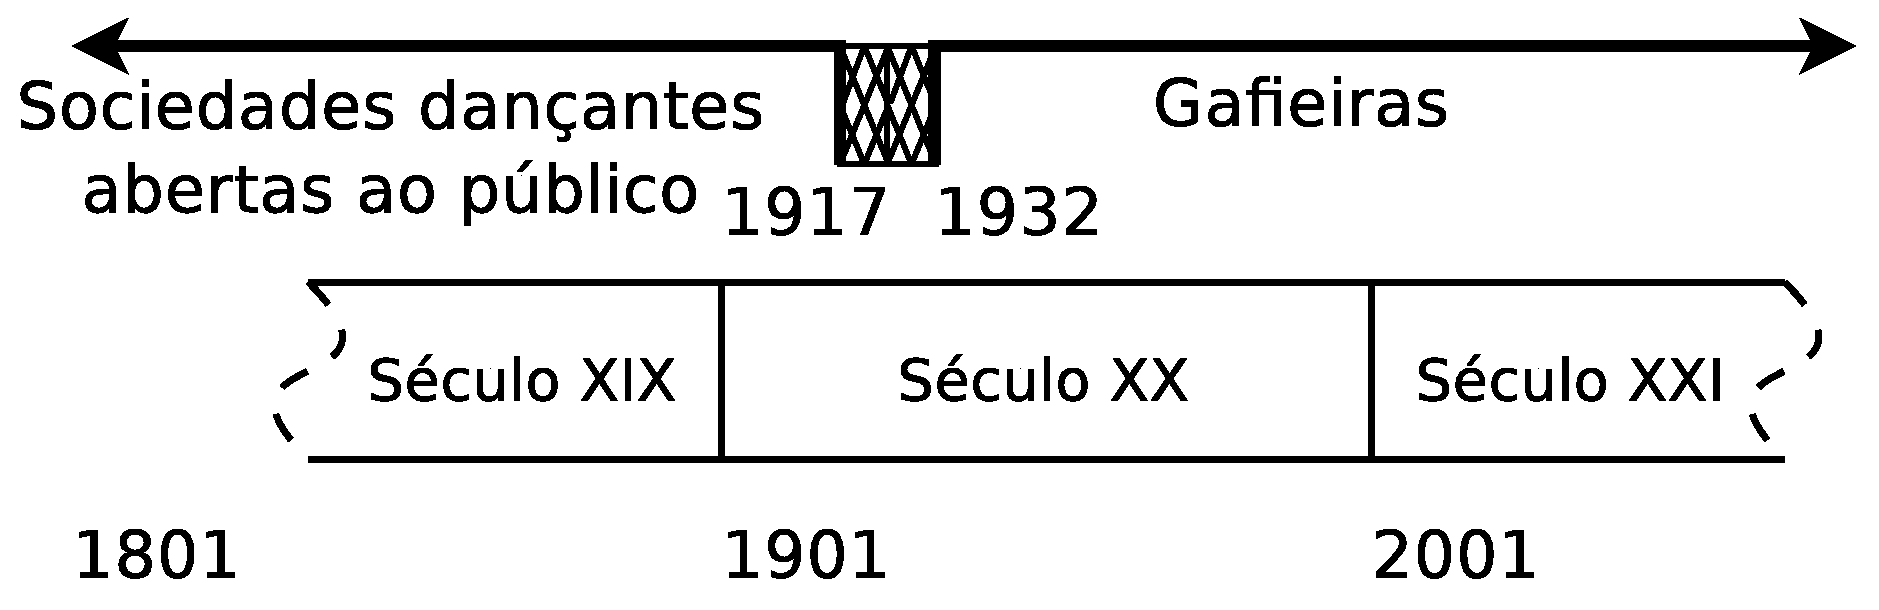
\includegraphics[width=1.0\textwidth]{chapters/cap-historia-gafieiras/gafieira-crono.eps}
  \caption{Cronologia da designação de gafieira para os salões de dança no Rio de Janeiro.}
  \label{fig:gafieiracrono}
\end{figure}

\PRLsep{Delitos vinculados com as gafieiras}

Podemos achar uma referencia ao termo gafieira no jornal ``O Radical'' (RJ),
no dia 8 de setembro de 1932 \cite[pp. 12]{gafieirajournaloradical1},
com o titular:
\begin{citando}%%
A sahida do baile: Por causa de Aracy, o estivador foi ferido á baia.\\
... Na rua Domingo Lopes, n. 243, em Madureira, está situado o club de dança Ideal, 
conhecido pelos moradores locaes por ``Gafieira''.
\end{citando} 
Ao dia seguinte, 9 de setembro de 1932, o jornal ``A Batalha'' (RJ), 
usava também a palavra ``gafieira'' para se referir ao mesmo incidente \cite[pp. 8]{gafieirajournalabatalha1}.

O ``Jornal do Brasil'', o dia 9 de janeiro de 1934, 
usa também a palavra gafieira \cite[pp. 11]{gafieirajournalbrasil1}, com o titular:
\begin{citando}%%
À porta de uma ``gafieira''.
Ainda o conflito da madrugada de domingo no largo de Madureira.
Faleceu um dos soldados no Hospital da Policia Militar. 
Ha no largo de Madureira uma sociedade dansante, mais conhecida por ``gafieira'', 
com entradas retribuidas, ondem de quando em quando, se registram conflitos, 
alguns de graves consequências...
\end{citando} 
Como é visto nas refecerias antes mostradas, e guardando semelhança com outras coincidências
posteriores que podem ser achadas na ``Biblioteca Digital da Fundação Biblioteca Nacional''; 
o termo gafieira, estava associado a lugares considerados perigosos;
isto propiciado pelo aumento do número de locais que se atribuíam este nome, junto com 
a diversidade e cultura  do seu público e administradores.
Porém, este não seria o padrão pelo qual se regiam todas as gafieiras, 
e certamente a conotação mais perigosa ou pejorativa iria mudando no tempo. 

\PRLsep{A gafieira limpa seu nome}

Por exemplo, sobre o Elite Club,  nos sabemos que funcionava as quintas, sábados e domingos,
e existia um fiscal no salão (o velho Russo)\cite[pp. 37]{gafieirajournalmanchete}, 
que fazia cumprir estritamente as normas de bom-tom, comportamento social e respeito ao ambiente, como todo clube familiar precisa ter \cite[pp. 12]{respeitojournalbrasil1}; de modo que, 
não eram admitidas damas que não estivessem de sapatos de salto alto \cite[pp. 37]{gafieirajournalmanchete};
homens embriagados não entravam e o traje indispensável era o paletó e gravata, 
ou no mínimo camisa fechada \cite[pp. 6 - cad. B]{entrevistajuliojournalbrasil1}.
O cavaleiro não podia abraçar a dama nem sentado na cadeira \cite[pp. 6 - cad. B]{entrevistajuliojournalbrasil1},
né dançar de rosto colado, ou por a mão nas costas da dama sem usar lenço \cite[pp. 10]{simoesjournalbrasil1}, 
quem fiscalizava, na porta, era um preto velho tratado por todos de ``titio''  \cite[pp. 37]{gafieirajournalmanchete}.
Se alguma regra não era cumprida, o seu Júlio, jogava a qualquer um para fora \cite[pp. 6 - cad. B]{entrevistajuliojournalbrasil1}.
Nos bailes dedicados ao padroeiro, todo 20 de janeiro, era obrigatório vestir de branco,
já seja no traje ou no vestido, incluindo sapatos e camisas \cite[pp. 37]{gafieirajournalmanchete}.
Tão grande era o censo de ordem dos frequentadores do Elite Club, 
que lhe era permitido operar estando a menos de 80 metros de um hospital,
sendo que nessa época existia a Lei n. 1.590 de 1924, 
seguindo a qual nenhuma casa de diversões podia estar a menos de 200 m de estabelecimentos hospitalares,
Ate o próprio Delegado Dulcídio Gonçalves, da Delegacia de Costumes,
dispensava-se de mandar policiar o Elite.
``À casa do Júlio não precisa de policiamento'', dizia o Delegado Dulcídio
\cite[pp. 5]{simoesjournalalutademocratica1}.


Assim, ao transcorrer dos anos, essa visão popular mais obscura da palavra gafieira foi mudando;
pelo qual o jornalista Francisco Duarte, o dia 12 de agosto de 1979,
escreve no Jornal do Brasil (RJ) sobre este assunto com o título:
``Gafieira - Tratado geral do ambiente que exige respeito'' \cite[pp. 10]{respeitojournalbrasil1}:
\begin{citando}%%
... o verbete Gafieira com o significado de baile reles, arrasta-pé, baile popular de baixa categoria.
No passado, encarada com má vontade pelos puristas do léxico e pela burguesia republicana dançante,
pode ter sido assim. Mas em 1979 -- e cabe aos dicionaristas verificar in loco --
gafieira é baile de clube particular, com entrada paga e freqüência livre, 
local de lazer e dança onde existe bom comportamento e muita compostura,
em perfeita integração racial.\\
(Francisco Duarte)
\end{citando}
Além da afirmação anterior, 
o jornalista explica como a ``Delegacia de Diversões Públicas'' classifica as casas de dança;
assim temos: 
\begin{itemize}
\item ``boates'', que são bar restaurantes com pista de dança e palco para show;
\item ``cabarés'', onde se bebe, come, dança e se tem espetáculos de variedades;
\item ``dancings'' onde se dança mediante pagamento em cartões e picotes; e 
\item ``inferninhos'' que são boates de baixa categoria, 
frequentados por pessoas de vida irregular e onde se toca música barulhenta.
\end{itemize} 
Em palavras de Duarte, ``Gafieiras são sinônimos de baile em salão espaçoso como boa música orquestral'' \cite[pp. 11]{respeitojournalbrasil1}.




%%%%%%%%%%%%%%%%%%%%%%%%%%%%%%%%%%%%%%%%%%%%%%%%%%%%%%%%%%%%%%%%%%%%%%%%%%%%%%%%
%% SUB SECTION
\section{Estatutos da gafieira}\index{Estatuto da Gafieira}
Os ``Estatutos da Gafieira'' é uma composição musical escrita, por Billy Blanco;
esta foi interpretada por primeira vez na voz de Inezita Barroso, 
numa gravação da "RCA Victor" em janeiro de 1954 \cite{musicaestatuto};
O seguinte texto mostra a letra da música numa 
versão publicada no jornal ``Cinelândia''  (RJ),
na segunda quinzena de dezembro de 1955 \cite[pp. 95]{musicaestatutojournal1955}.
\begin{citando}%%
\center{Moço! Olha o vexame!}\\
O ambiente ``ingige'' respeito!\\
Pelos estatutos da nossa gafieira\\
Dance a noite inteira, mas dance direito!\\
Aliás, pelo artigo 120,\\
O cavalheiro que fizer o seguinte:\\
Subir nas paredes, dançar de pé pro ar,\\
Morar na bebida sem querer pagar,\\
Abusar da umbigada de maneira folgazã,\\
Prejudicando hoje o bom crioulo de amanhã,\\
Será distintamente censurado!\\
Se balançar o corpo, tá na mão do delegado!\\
Balançou o corpo? tá na mão do delegado!\\
\end{citando}
O texto é uma tentativa bem-humorada do autor de descrever o que acontecia 
nas gafieiras, porém na época da escrita desta popular samba, não
existiam tais estatutos\footnote{Estatutos, no sentido de regulamento, 
ordenança o conjunto de normas legais pelas que se regula o funcionamento de uma corporação ou associação.};
existia um código de costumes sim \cite[pp. 13]{respeitojournalbrasil1} em alguns salões, 
mas cada casa de dança imponia estes no seu local a critério do fiscal do salão ou dos 
donos \cite[pp. 10]{simoesjournalbrasil1} \cite[pp. 6 - cad. B]{entrevistajuliojournalbrasil1} \cite[pp. 37]{gafieirajournalmanchete},
isto é confirmado por um depoimento realizado por 
Billy Blanco no 8 de julho de 2011 \cite[pp. 56]{depoimentobilly}; o texto a seguir
mostra um fragmento dessa entrevista.

\begin{citando}%%
"Observando os acontecimentos de uma gafieira, então, eu imaginei
coisas, porque o compositor vive muito da imaginação. E eu criava situações 
possíveis de serem acontecidas na gafieira, ou então narrava o que
acontecia realmente. Por exemplo, no [samba] Pistom de Gafieira, tinha
um cidadão que era pistonista da orquestra que sempre tocava forte para
disfarçar quando a polícia vinha chegando. Doutra feita, eu tive a ideia
de fazer o estatuto para a gafieira. Então eu humorizei, porque ninguém
dança de pé pro ar, nem sobe em parede, não é? Mas a gente cria uma
extravagância dessas para dar uma certa graça, um certo sentido à música.
Na época, não havia código nenhum, eu apenas criei aquilo e muitas gafieiras 
depois tinham esse estatuto na parede para quem quisesse cantar.
Você vê que as regras do estatuto são umas regras brincalhonas, não é?" 
~\\
(Billy Blanco)
\end{citando}

Mesmo observando que as regras propostas pelo autor tem um caráter humorístico e sarcástico,
o texto foi adotado rapidamente pelas gafieiras, como um chamado a reflexão sobre umas
normas básicas a serem tidas em conta no salão, pois tem um grau de bom senso. Por exemplo: 
A linha 7, pode ser interpretada como uma indicação a 
não fazer movimentos aéreos na pista de dança,
ou  evitar movimentos capoerísticos; tudo isto
pelo evidente espacio reduzido e compartilhado que existe na pista de dança, 
além de que os movimentos aéreos estão pensados para ser
executados em apresentações e não em danças sociais. 
A linha 8, nos lembra o respeito ao parceiro; pois a pessoa que dança precisa
estar no controle de suas faculdades físicas e mentais; 
no caso dos \hyperref[def:Condutor]{\textbf{condutores}}\footnote{\label{footlab:conducao}Nas danças sociais é comumente usado o paradigma da condução; 
no qual, no casal, uma pessoa assume o papel de \hyperref[def:Condutor]{\textbf{condutor}} dos movimentos e 
a outra pessoa assume o papel de \hyperref[def:Seguidor]{\textbf{seguidor}}, este recebe a informação da condução e retorna uma resposta corporal.}, 
para estar atentos ao salão e cuidar do seu par enquanto os movimentos são executados, 
e no caso do \hyperref[def:Seguidor]{\textbf{seguidor}}\footref{footlab:conducao} para evitar problemas
nos giros e outros movimentos que precisem  controle do eixo do corpo.
As linhas 9 e 10 indicam sobre um conjunto de expressões artísticas 
afro-brasileiras emolduradas no século XIX com o nome de ``samba umbigada'' \cite[pp. 47]{diniz2008almanaque} \cite[pp. 85]{sandroni2001feitico}; nestas danças existe
um movimento chamado ``umbigada'' \cite[pp. 50]{da2015historia} que dá nome à dança, na qual o ventre do homem e da mulher batem geralmente para indicar
a troca de dançarino; assim as linhas 9 e 10 se referem a
 evitar ``abusar'' de movimentos de umbigada que provem de danças que não eram bem vistas na época e eram consideradas gentílicas \cite[pp. 85]{sandroni2001feitico}.
Finalmente,
a linha 12 fala sobre balançar o corpo, que seguindo o contexto cultural, 
pode indicar não agir como bêbado\footnote{``Balançar o corpo; agitar, como o bebado, mal firme, e outros táes'', Diccionario da lingua portugueza, 1858 \cite[pp.296]{diccionario1858}.}, ou em outras palavras,
com pouca elegância ou respeito,
caso contrario seria levado à delegacia!.



%%%%%%%%%%%%%%%%%%%%%%%%%%%%%%%%%%%%%%%%%%%%%%%%%%%%%%%%%%%%%%%%%%%%%%%%%%%%%%%%
%% Capitulo
%%%%%%%%%%%%%%%%%%%%%%%%%%%%%%%%%%%%%%%%%%%%%%%%%%%%%%%%%%%%%%%%%%%%%%%%%%%%%%%%
\chapterimage{chapter_head_2.pdf} % Chapter heading image

\chapter{Historia da música do samba}\index{Música do samba}

O samba é uns dos gêneros musicais mais conhecidos no Brasil do século XXI;
entre estes gêneros mais populares, temos por exemplo, ao ``forró'' e ao ``Sertanejo'';
sendo que o samba se distingue entre eles, 
como a principal expressão popular da música brasileira \cite[pp. 47]{diniz2008almanaque}.\\


%\begin{definition}[Samba:]
\begin{remarcar}
\textbf{Samba:}
\index{Samba}
\label{ref:samba} 
No Brasil, a palavra samba  é usada como designação de uma dança popular  e música  em compasso binário (basicamente 2/4), 
de ritmo sincopado e andamento variado \cite[pp. 290]{dourado2004dicionario} \cite[pp. 684]{marcondes1977enciclopediav2};
ambos com uma forte influencia da cultura africana \cite[pp. 290]{dourado2004dicionario};
representando estas desde inícios do século XX, 
uma expressão cultural, urbana e popular no Brasil \cite[pp. 684]{marcondes1977enciclopediav2} \cite[pp. 290]{dourado2004dicionario}.
\end{remarcar}
%\end{definition}

A popularização, o reconhecimento comercial e a representatividade cultural no consciente coletivo do brasileiro,
não sempre estiverem alinhados com o samba, 
sendo que esta conjunção teve seu origem a inícios do seculo XX, 
com o inicio das gravações comerciais, em disco, e a consequente popularização comercial do gênero.

 As reuniões na casa da Tia Ciata foram o cenário da criação do samba-maxixe ``Pelo telefone'',
 composto, em 1916, 
por Ernesto dos Santos (Donga) e Mauro de almeida (Peru dos Pés Frios) \cite[pp. 34]{diniz2006almanaque} \cite[pp. 49]{diniz2008almanaque} \cite{musicapelotelefone} \cite[pp. 28]{diniz2003almanaque}.
\begin{remarcar}
Dados da música \textbf{Pelo telefone}:
\index{Pelo telefone}
\begin{itemize}
\item 1996, novembro 6, é presentada uma petição de registro no
Departamento de Direitos Autorais, da Biblioteca Nacional, 
do Rio de Janeiro (RJ), 
por   Ernesto dos Santos  para o samba carnavalesco \textbf{Pelo telefone} \cite[pp. 599]{marcondes1977enciclopediav2}.
\item 1996, novembro 16, Ernesto dos Santos, 
anexa à petição um atestado que afirma que 
o samba carnavalesco \textbf{Pelo telefone}, 
foi executado em público pela primeira vez no
Cine-Teatro Velho o dia 25 de outubro de 1916,
este atestado foi subscrito por M.P. Cabrita e Julio Suckow \cite[pp. 599]{marcondes1977enciclopediav2}.
\item 1996, novembro 27, o registro foi efetivado com o número 3.295 \cite[pp. 599]{marcondes1977enciclopediav2}.
\item 1996, dezembro 16, a partitura manuscrita para piano, feita por Pixinguinha, 
estava dedicada a Mauro de Almeida e Norberto Amaral (Morcego) é
publicada no Instituto de Artes Gráficas, do Rio de Janeiro \cite[pp. 599]{marcondes1977enciclopediav2}.
\item Carnaval de 1917, a música foi sucesso   \cite[pp. 599]{marcondes1977enciclopediav2}  \cite[pp. 35]{diniz2006almanaque}, 

\item 1917, É realizada a primeira gravação de  \textbf{Pelo telefone}, feita pela Banda Ondeon (121.313-B), 
onde consta como autor unicamente Donga, 
sendo esta uma gravação instrumental \cite{musicapelotelefone} \cite[pp. 599]{marcondes1977enciclopediav2},
e  fabricada especialmente para a Casa Edison, pela fabrica Ondeon, com número de patente 3465.
\item 1917, É realizada a segunda gravação, onde os versos de \textbf{Pelo telefone} seriam conhecidos pelo público;
foram encargados da interpretação, ``Bahiano\footnote{Está 
escrito Bahiano na capa do disco, porem muita referencias bibliográficas,
escrevem Baiano.} e côro'' (121.322-A), acompanhado somente de violão e cavaquinho. 
Esta gravação é fabricada especialmente para a Casa Edison, pela fabrica Ondeon, com número de patente 3465,  
e constam como autores Donga e Mauro de Almeida 
(música e letra respetivamente) \cite[pp. 599]{marcondes1977enciclopediav2} 
\cite[pp. 35]{diniz2006almanaque}  \cite{musicapelotelefone}.
\end{itemize}
\end{remarcar}

Porem, esta autoria é questionada por compositores contemporâneos de Donga, que alegam que
ele modificou e apropriou-se de uma criação coletiva e anônima, 
de tradição oral cantada por todos na casa da Tia Ciata \cite{musicapelotelefone} \cite[pp. 35]{diniz2006almanaque} \cite[pp. 49]{diniz2008almanaque};
assim, o dia 4 de Fevereiro de 1917, no ``Jornal do Brasil'' (RJ), Tia Ciata, Sinhô e outros,
protestaram a usurpação da autoria, parodiando à versão gravada, como é visto a seguir \cite[pp. 17]{TiaCiataVsDonga} \cite[pp. 118-119]{sandroni2001feitico}:
\begin{citando}%%
\begin{center}
1ra PARTE\\
Pelo telefone a minha boa gente\\
Mandou-me avisar!...\\
Que meu bom arranjo era oferecido\\
Para se cantar!...\\
~\\
2da PARTE\\
Ai! Ai! Ai!... leve a mão\\
A' consciencia!...\\
Meu bem,\\
Ai! Ai! Ai!... porque\\
Tanta presença!...\\
Meu bem!\\
~\\
1ra PARTE\\
O que cara dura de dizer nas rodas\\
Que este arranjo é teu?...\\
É do bom Hilario e da velha Ciatta\\
Que o Sinhô escreveu!...\\
~\\
3ra PARTE\\
Tomara que tu apanhes,\\
Para não tornar a fazer isso,\\
Escrever o que é dos outros,\\
Sem olhar o compromisso.
\end{center}
\end{citando}%%

Por outro lado, durante muito tempo ``Pelo telefone'' foi considerado o primeiro samba gravado;
porem, segundo Flávio Silva  já existiam outros discos anteriormente com a etiqueta samba,
inclusive pela Casa Edison, que gravou ``pelo telefone''  \cite[pp. 96]{hertzman2013making} \cite[pp. 118]{sandroni2001feitico}.

Apesar de todos estes problemas, há uma contribuição de ``Pelo telefone'' à música, 
esta foi a indicação do gênero ``samba'' no selo do disco junto ao registro na Biblioteca Nacional,
que abriu o caminho para à difusão comercial e urbanização do gênero samba,
 e seu consequente prestigio \cite{musicapelotelefone} \cite[pp. 49]{diniz2008almanaque};
como corrobora Flávio Silva, que no seu levantamento bibliográfico deteta que, no carnaval, o termo
samba aparece na prensa  de Rio de Janeiro \cite[pp. 118]{sandroni2001feitico}, 
\begin{itemize}
\item 3 vezes em 1916, 
\item 22 vezes em 1917 e
\item 37 vezes em 1918.
\end{itemize}

\section{Qual é a família do samba (música)?}
\begin{remarcar}
\index{Batucada}
\index{Música do samba!Batucada}
\textbf{Batucada (música):} É a denominação dada ao ritmo do 
\hyperref[ref:batuquedanca]{\textbf{batuque}}\footnote{Para 
mais informação sobre o batuque ir a páginas \pageref{ref:batuquedanca1800} e \pageref{ref:batuquedanca}.} 
e é também usado como sinônimo deste \cite[pp. 89]{marcondes1977enciclopedia}.
\end{remarcar}
Existem muitos subgêneros em que o samba é tocado e cantado, alguns tiveram vida efêmera,
e outros perduraram no tempo, a continuação serão listados alguns destes subgêneros.

\begin{description}

%% MARACATU


\item[Bossa nova:] 
\index{Música do samba!Bossa nova}
\index{Música do samba!Samba-bossa}
Também chamado \textbf{samba-bossa}, este gênero pode ser entendido como um samba-choro modernizado \cite[pp. 63]{reinato2010musica}.
A bossa nova surgiu  na década de 1950 \cite[pp. 130]{perna2002samba},
apos a segunda gerra mundial pela influencia da cultura norte-americana, motivada 
pela política desenvolvimentista do presidente do Brasil, Juscelino Kubitschek (1956 - 1961) \cite[pp. 15]{de2003tem}.
Esta variante do samba é caraterizada por uma sofisticada harmonia e um modo diferente de dividir o fraseado, 
agregando influencias do impressionismo erudito do jazz  \cite[pp. 130]{perna2002samba} \cite[pp. 15]{de2003tem}. 

O inicio da bossa nova, e sua popularização, 
marcou um período de dificuldade para o choro e seus instrumentistas,
pelo desinteresse  do choro ao ser considerada coisa de velho, quadrada, nacionalista, de aposentado e suburbano \cite{rizzi2016musica}.

A bossa nova foi inaugurada usando composições e interpretações de, Antônio Carlos Jobim (Tom Jobim) e Carlos Lyra,
a poesia de Vinícius de Moraes, e
a batida do violão de João Gilberto \cite[pp. 130]{perna2002samba}  \cite[pp. 15]{de2003tem}.
\begin{example} ~

\begin{itemize}
\item ``Chega de saudade'' (1958) de Vinícius de Moraes e Antônio Carlos Jobim \cite{castro2016chega} \cite{tomjobim}.
\item ``Garota de Ipanema'' (1962) de Vinícius de Moraes e Antônio Carlos Jobim \cite{tomjobim}.
\end{itemize}
\end{example}

\item[Choro:] 
\index{Música do samba!Choro}
Este é um gênero musical brasileiro, surgido na cidade de São Sebastião, Rio de Janeiro, por volta de 1870 \cite[pp. 14]{diniz2003almanaque} \cite[pp. 132]{perna2002samba} \cite[pp. 64]{reinato2010musica},
com espirito melancólico que mesclou o samba com  estilos europeus como schottisches, polcas,
valsas e outros gêneros em voga na época  \cite[pp. 64]{reinato2010musica} \cite[pp. 79]{dourado2004dicionario} \cite[pp. 132]{perna2002samba}.
O choro ou chorinho é uma composição livre, em ritmo binário, 
tradicionalmente composto em três seções com 16 compassos cada uma \cite[pp. 64]{reinato2010musica}.
Para o ano de 1910 este já era um gênero consolidado \cite[pp. 12]{diniz2003almanaque}.

Entre os instrumentos mais populares que constituíram o choro na época da criação, 
estão o violão, o cavaquinho e a flauta transversal;
na década de 1930 foram incorporados, o pandeiro, o bandolin e a clarineta \cite[pp. 64]{reinato2010musica} \cite[pp. 79]{dourado2004dicionario} \cite[pp. 132]{perna2002samba};
todos estes instrumentos dão à música um aspecto sentimental melancólico e ``choroso'', e
é de ali que alguns autores apontam que surge o nome do estilo \cite[pp. 132]{perna2002samba};
porem, seguindo Batista Siqueira, 
o termo choro vem da fusão do verbo ``chorar'' e ``chorus'', coro em latim \cite[pp. 13]{diniz2003almanaque}.

O flautista, Joaquim Callado (Joaquim Antônio da Silva Callado 1848-1880) 
é conhecido como ``O pai do choro'';
este foi o autor de 66 melodias, e conseguiu conciliar: 
uma sólida formação musical com um grande poder de improvisação  \cite[pp. 15]{diniz2003almanaque} \cite[pp. 64]{reinato2010musica}.
Entre os grandes interpretes do gênero temos a:
Pixinguinha, Waldir Azevedo, Jacó do Bandolim, Dinho Sete Cordas, Altamiro Carillo \cite[pp. 79]{dourado2004dicionario}, etc.

\begin{example} ~

\begin{itemize}
\item ``A flor amorosa'' de Joaquim Callado \cite[pp. 8]{livingston2005choro} \cite[pp. 15]{diniz2003almanaque}.
\item ``Cruzes, minha prima'' de Joaquim Callado \cite[pp. 15]{diniz2003almanaque}.
\item ``Querida por todos'' de Joaquim Callado \cite[pp. 15]{diniz2003almanaque}.
\item ``Tico-Tico no fubá'' (1917) de Zequinha de Abreu, sem letra e chamado na época ``Tico-Tico no farelo'' \cite[pp. 6]{marcondes1998enciclopedia} \cite[pp. 39,91]{diniz2003almanaque}
\item ``Carinhoso'' (1927) Pixinguinha   \cite[pp. 133]{perna2002samba}.
\item ``Brasileirinho'' (1947) de Valdir Azevedo  \cite[pp. 133]{perna2002samba}.
\item ``Noites cariocas'' Jacob do Bandolim \cite{diniz2003almanaque}.
\item ``Doce de coco'' Jacob do Bandolim \cite{diniz2003almanaque}.
\item ``Vibrações'' Jacob do Bandolim \cite{diniz2003almanaque}.
\item ``Melodia celestial'' de Raul Barros \cite[pp. 130]{livingston2005choro}.
\end{itemize}
\end{example}

\item[Marchinha:] 
\index{Música do samba!Marchinha}
\index{Música do samba!Marcha}
Também chamado \textbf{marcha} \cite[pp. 448]{marcondes1977enciclopedia},
é um gênero de música popular, em compasso binário (2/4) de andamento vivo, 
está provem dos ranchos e cordões carnavalescos, a coreografia consiste num andar ritmado e em voltas. \cite[pp. 65]{reinato2010musica}.

A diferença entre a marcha-rancho e  a marchinha está no jeito cadenciado, 
melodioso e harmônico da primeira, em contrapartida ao estilo espevitado,
jocoso, cheio de sátiras e com letras de duplo sentido da segunda \cite[pp. 84,87]{diniz2008almanaque}.

A primeira marchinha carnavalesca, titulada ``Ô abre alas'', foi escrita em 1899 por Chiquinha Gonzaga \cite[pp. 84, 239]{diniz2008almanaque}.

\begin{example} ~

\begin{itemize}
\item ``Ô abre alas'' (1899) Chiquinha Gonzaga  \cite[pp. 84, 239]{diniz2008almanaque}.
\item ``Os calças-largas'' (1927) Lamartine Babo e Francisco Gonçalves de Oliveira,
interpretado por Frederico Rocha \cite[pp. 91]{diniz2008almanaque}.
\item ``O teu cabelo não nega'' (1932) de Lamartine Babo e dos Irmãos Valença, interpretado por Castro Barbosa \cite[pp. 99]{diniz2008almanaque}.
\item ``Balancê'' (1936) de Alberto Ribeiro e Braguinha interpretado por Carmen Miranda \cite[pp. 83]{diniz2008almanaque}.
\item ``Mamãe, eu quero'' (1937) de Vicente Paiva e Jararaca \cite[pp. 584]{marcondes1977enciclopediav2} \cite[pp. 93]{diniz2008almanaque}.
\item ``Cabeleira do Zezé'' (1964) de João Roberto Kelly e Roberto Faissal interpretado por Jorge Goulart \cite[pp. 117,118]{diniz2008almanaque}.
\item ``Pierrô apaixonado'' (1936) de Heitor dos prazeres e Noel Rosa \cite[pp. 1070]{marcondes1977enciclopediav2} \cite[pp. 53]{diniz2008almanaque}.
\end{itemize}
\end{example}

\item[Marcha-rancho:] 
\index{Música do samba!Marcha-rancho}
Inicialmente chamado de \textbf{marcha de rancho} \cite[pp. 448]{marcondes1977enciclopedia}
é um gênero de musica popular, em compasso binário andante, 
está provem da musica produzida pelas chamadas orquestras dos ranchos e cordoes 
carnavalescos de fins da década de 1910 \cite[pp. 65]{reinato2010musica} \cite[pp. 448]{marcondes1977enciclopedia}.
A marcha-rancho tem um ritmo mais dolente que o das marchas (marchinhas)
e tem muito mais trabalho na parte melódica. 
Este gênero foi desenvolvido por autores reconhecidos, 
a finais da década de 1920;
onde podemos ver composições como a marcha rancho com coro ``moreninha'',
gravada no disco Ondeon n. 123.208, em 1927 \cite[pp. 448]{marcondes1977enciclopedia}.

\begin{example} ~

\begin{itemize}
\item ``Moreninha'' (1927) de Eduardo Souto \cite[pp. 448]{marcondes1977enciclopedia}
%\item ``Bem-te-vi'' (1933) de Lamartine Babo interpretado por Gastão Formenti \cite[pp. 916]{marcondes1977enciclopediav2} \cite[pp. 87]{diniz2008almanaque}.
\item ``As Pastorinhas'' (1938) de Carlos Alberto Ferreira Braga (Braguinha ou João de Barro) e Noel Rosa, 
inicialmente titulado ``Linda pequena''.
Apos modificação de nome, letra e música, 
foi regravado e interpretado por Sílvio Caldas \cite[pp. 1066]{marcondes1977enciclopediav2} \cite[pp. 87]{diniz2008almanaque}.
\item ``Marcha da quarta-feira de cinzas'' (1962) de Vinícius de Moraes e Carlos Lyra \cite[pp. 1021]{marcondes1977enciclopediav2} \cite[pp. 91]{diniz2008almanaque}.
\item ``A banda'' (1966) Chico Buarque interpretada por Nara Leão \cite[pp. 90]{diniz2008almanaque}.
\item ``Máscara negra'' (1967) José Flores de Jesus (Zè Kéti)  \cite[pp. 89]{diniz2008almanaque}.
\item ``Flor do sereno'' (2000)  \cite[pp. 88]{diniz2008almanaque}.

\end{itemize}
\end{example}

\item[Maxixe:] 
\index{Música do samba!Maxixe}
Também chamado \textbf{machiche}\footnote{Seguindo Batista Siqueira, 
o termo maxixe é uma corruptela de ``Macho, viche'', 
de ``sou macho, virgem'', e por conseguinte devia ser escrito machiche \cite[pp. 198]{dourado2004dicionario}.}.
Na época se acreditava que o nome seria em aluição de uma fruta que brotava junto ao capim dos piores recantos cariocas,
como a zona de baixo meretricio do Mangue do Rio de Janeiro \cite[pp. 198]{dourado2004dicionario}.
O maxixe designou durante certo tempo à música brasileira característica da cidade, 
ate que cedeu seu lugar ao samba \cite[pp. 4]{musicasambavariasdef1}.

O maxixe é composto de ritmos sincopados, com ascendência de ritmos africanos \cite[pp. 198]{dourado2004dicionario}.
Esta é uma música afro-brasileira \cite[pp. 4]{musicasambavariasdef1} 
que foi criada para dar contexto ao  maxixe (dança), que já existia e era dançado em vários gêneros musicais da época.
O maxixe (música) só foi reconhecida pelas casas musicais como um gênero musical no final do seculo XIX \cite[pp. 465]{marcondes1977enciclopedia}. 
Este gênero resultou da fusão do ritmo do tango e a havanera, 
do andamento da polca e a sincopa de músicas com ascendência africana como o lundu  \cite[pp. 29]{efege1974maxixe}  \cite[pp. 465]{marcondes1977enciclopedia}. 

O primeiro maxixe impresso com a respectiva menção de gênero, é ``Ora bolas!'' de Juca Storoni em 1897,
sendo este nome um pseudônimo, o que da uma indicação do estigma da época aos compositores deste gênero \cite[pp. 80]{sandroni2001feitico} \cite[pp. 108]{efege1974maxixe}.

\begin{example} ~

\begin{itemize}
\item ``Ora, bolas!'' (1897) de Juca Storoni \cite[pp. 108]{efege1974maxixe}.
\item ``Gaucho (Corta-Jaca)'' (1897) de Chiquinha Gonzaga \cite{reportagemtvmaxixe} \cite[pp. 30]{efege1974maxixe}.
\item ``Maxixe da Guarda Velha'' (1899) com letra de Arthur Azevedo, 
e música do compositor paulista Nicolino Milano  \cite{reportagemtvmaxixe}. 
\item ``Maxixe Aristocrático'' (1904) de José Nunes \cite{REIS2003}.
\item ``Vem cá, mulata'' (1906) de José do Patrocínio Filho, Chicot e Thoreau \cite{REIS2003}.
\item ``Forrobodó'' (1912) de Chiquinha Gonzaga \cite{REIS2003} \cite{reportagemtvmaxixe}.
\item ``Jocotó'' Roque V. Vieira \cite{reportagemtvmaxixe}.
\end{itemize}
\end{example}

\item[Pagode:] 
\index{Música do samba!Pagode}
Também chamado \textbf{samba de fundo do quintal}  \cite[pp. 130]{perna2002samba}.
No Rio de Janeiro, pagodes são locais de reunião informal, quintais cobertos, e outros,
que davam espaço a um pequeno baile pre carnavalesco, 
rodas de samba ou de partido-alto, criadas geralmente por músicos amadores \cite[pp. 130]{perna2002samba} \cite[pp. 241]{dourado2004dicionario} \cite[pp. 241]{dourado2004dicionario}.
Assim, nestos locais se cantavam ritmos populares principalmente samba,
geralmente acompanhados de percussão, cavaquinho e violão, 
de modo que este  estilo de fazer música passou a ser chamado de pagode \cite[pp. 63]{reinato2010musica}  \cite[pp. 130]{perna2002samba}.

Ao final da década de 1960 saíram os primeiros sambistas classificados como pagodeiros,
porem a origem do pagode seria anterior a este período \cite{sedano2018bezerra}.
Os sambistas de Rio de Janeiro desde os tempos da Tia Ciata, 
falavam pagode para designar ao samba de forma carinhosa; 
assim, samba e pagode era entendido como uma coisa só, uma festa, 
onde as pessoas se reuniam, cantavam, dançavam, comiam e ate paqueravam \cite[pp. 209]{diniz2006almanaque}.

O bloco carnavalesco ``Cacique de Ramos'' teria sido o centro irradiador do pagode no final da década de 1960,
sendo este o promotor do ressurgimento do gênero no cenário musical brasileiro \cite{sedano2018bezerra},
com seus reuniões  para um pagode todas as quartas feiras  \cite[pp. 210]{diniz2006almanaque}.

Apos o ano 1970 a industria da música no Brasil sofreu uma crise que afetou a produção musical, 
incluindo ao pagode;
porem a partir do ano de 1981, o mercado musical retomou seu interesse pelo pagode \cite{sedano2018bezerra}.
com nomes como: Zeca Pagodinho, Agepê, Almir Guineto, Alicione, 
Jorge Aragão e Jovelina Pérola Negra \cite[pp. 130]{perna2002samba} \cite{sedano2018bezerra};
sendo, ``fundo de quintal'' (1980), o primeiro ``grupo'' de pagode \cite[pp. 130]{perna2002samba} \cite{fundodequintal}.

Em 1985, a gravadora RGE lançou o LP chamado  ``Raça brasileira'', 
sendo este projeto mas que uma coletânea, um marco fonográfico e cultural,
do fenômeno conhecido como pagode. Este projeto contou com a colaboração de artistas como:
Zeca Pagodinho, 
Jovelina Pérola Negra, 
Eliane Machado,
Pedrinho da Flor e
Mauro Diniz \cite[pp. 211]{diniz2006almanaque}.

Estes artistas antes identificados como pagodeiros, mudaram seu status em 1990, 
 quando apareceram grupos de ``pagode romântico'', 
de modo que os pagodeiros da antiga passaram a chamar-se como ``sambista de raiz''  \cite{sedano2018bezerra}. 

\begin{example} LP ``Raça brasileira'' lançado em 1985:

\begin{itemize}
\item ``Raça Brasileira'' interpretado por Elaine Machado.
\item ``Leilão'' interpretado por Zeca Pagodinho.
\item ``Que Maravilha (Maravilhas do Amor)'' interpretado por Pedrinho Da Flor.
\item ``Feirinha da Pavuna (Confusão de Legumes)'' interpretado por Jovelina Pérola Negra.
\item ``Mal de Amor''  interpretado por  Mauro Diniz.
\item ``Pot-Pourri Santa Paciência/Bamba de Berço'' interpretado por Zeca Pagodinho, Mauro Diniz.
\item ``Garrafeiro'' interpretado por Zeca Pagodinho.
\item ``Pingueira'' interpretado por Elaine Machado.
\item ``Ingrata Paixão'' interpretado por Mauro Diniz.
\item ``Pomba-Rolou'' interpretado por  Jovelina Pérola Negra.
\item ``A Vaca'' interpretado por Zeca Pagodinho.
\item ``Pot-Pourri Pedra No Caminho/Bagaço da Laranja'' interpretado por Zeca Pagodinho, Jovelina Pérola Negra e Pedrinho Da Flor.
\end{itemize}
\end{example}

\item[Sambalanço:]
\label{ref:sambalanco}
\index{Música do samba!Samba balanço}
\index{Música do samba!Sambalanço}
O sambalanço e um gênero musical,
que se encontra num ponto intermédio entre o samba tradicional (de morro e batucada)
e a bossa nova (samba estilizado), e surgiu na década de 1950 \cite[pp. 119]{diniz2008almanaque}.
Onde vários compositores, interpretes e músicos, 
transformaram a bossa nova dando-lhe maior impacto rítmico e uma nova estrutura instrumental,
numa amalgama que agora conhecemos como sambalanço, \textbf{balanço} ou \textbf{samba de balanço} \cite{de2017sambalanco}.

Carlos Lyra procurando uma denominação para sua música, 
pois achava que esta já não tinha direito de ser chamado de bossa nova,
achou no termo sambalanço, mescla de samba e balanço, a designação mais apropriada para esta \cite{castro2011bossa};
este nome foi inscrito por ele no registro de marcas e patentes \cite[pp. 127]{vianna1999bezerra} \cite{castro2011bossa}.


Carlos Lyra lança em 1961  seu segundo LP \cite[pp. 142]{lyrasongbook}  \cite{castro2011bossa}, 
tendo nesta ocasião a colaboração de Vinícius de Moraes,
este último, escreve na contra portada do LP um comentário sobre Lyra e o sambalanço,
indicando que a música de Carlos, pertence à corrente mais nacionalista da bossa nova,
pelo qual este sentiu a necessidade de dar um nome próprio a sua obra, 
chamando-o de sambalanço, 
porem Vinícius questiona a necessidade do nome e reafirma que a expressão 
 bossa nova tem a amplitude necessária para cobrir sem espirito de divisão esta música \cite{castro2011bossa}.

Segundo Orlandivo o sambalanço é ``uma música que tira você, nem que fique em pé dançando sozinho ali'';
sendo este estilo muito diferente da bossa nova, pois nesta última por mais que você queira dançar, fica difícil;
a bossa nova é uma música para escutar sentado \cite{de2017sambalanco}.
\begin{example} ~

\begin{itemize}
\item ``Era Bom'' (1960) de Hianto de Almeida e Macedo Neto  \cite[pp. 123]{de2003tem}.
\item ``Só amor'' (1961) de Vinícius De Moraes no segundo LP de Carlos Lyra \cite[pp. 142]{lyrasongbook}  
\item ``Tem que balançar'' (1961) de Carlos Imperial  \cite{de2017sambalanco}.
\item ``Gamação'' (1962) de João Roberto Kelly \cite[pp. 122]{de2003tem}.
\item ``Só vou de balanço'' (1963) de João Roberto Kelly \cite{de2017sambalanco}.
\item ``Na Roda do Samba'' (1964) de Orlandivo e Helton Menezes \cite{de2017sambalanco} \cite[pp. 122]{de2003tem}.
\item ``Toque Balanço, Moço!'' (1965) de Roberto Carlos e Erasmo Carlos \cite{de2017sambalanco} \cite[pp. 123]{de2003tem}.
\end{itemize}
\end{example}

\textbf{Sambalanço da década de 1990:} Também chamado \textbf{pagode paulista}  \cite[pp. 130]{perna2002samba}.
Durante os anos de 1994 e 1995, 
foi usado pela mídia o termo sambalanço, para designar a um certo tipo de música, 
bem diferente estilisticamente ao de 1950;
sendo este novo sambalanço um pagode relacionado a uma identidade nacional,
com uma atenção maior da mídia a este novo gênero \cite[pp. 127]{vianna1999bezerra}, 
e influenciada pela ``soul music'' norte-americana e a música romântica dos grupos sertanejos da época  \cite[pp. 130-131]{perna2002samba}.
Dentro desse novo sambalanço podemos ver grupos originários de São Paulo como, Raça negra e o Grupo Raça;
e ao grupo originário de Minas Gerais: Só pra contrariar \cite[pp. 130]{perna2002samba} \cite[pp. 128]{vianna1999bezerra}.
Outros nomes relativos a este pagode são: Arte Popular, Grupo Sensação, Katinguelê, Exaltasamba, etc.

\begin{example} ~

\begin{itemize}
\item ``Pra que mentir'' disco lançado em 1991 por Raça negra.
\item ``Cigana'' disco lançado em 1992 por Raça negra.
\item ``Cheia de manias'' disco lançado em 1992 por Raça negra.
\item ``Doce paixão'' disco lançado em 1993 por Raça negra.
\item ``É no pagode'' interpretado por Arte Popular.
\end{itemize}
\end{example}



\item[Samba-bolero:] 
\index{Música do samba!Samba-bolero}
\index{Música do samba!Sambolero}
Também chamado \textbf{sambolero}.
Este é um gênero surgido nos anos 1950, e foi uma tentativa de aproximar o samba tradicional com o bolero,
que dominava os salões de dança do Rio de Janeiro e de São paulo na época \cite[pp. 291]{dourado2004dicionario}.
O sambolero era uma samba-canção com ritmo ``abolerado'' \cite[pp. 685]{marcondes1977enciclopediav2},
porem o termo inciou a desaparecer ao redor de 1963, 
quando a bossa nova ia sendo adotado pelo público \cite[pp. 84]{biblioteca2006cultura}.

\begin{example} ~

\begin{itemize}
\item ``Pobre Menino Rico'' (1955) interpretado  por Lana Bitencourt \cite[pp. 5]{pobremeninorico}.
\item ``Canção de volta'' (1958) interpretado por Carlos José \cite[pp. 36]{carlosjose}.
\item ``Molambo'' (1956) de Jayme Florence e Augusto Mesquita \cite[pp. 481, 516]{faour2001bastidores}.
\item ``Sambolero'' interpretado por Luiz Bonfá \cite[pp. 49]{sambolero}.
\end{itemize}
\end{example}


\item[Samba de breque:] 
\index{Música do samba!Samba de breque}

Expressão cunhada, em 1936, por Moreira da silva a partir da gravação de ``Jogo proibido'' \cite[pp. 291]{dourado2004dicionario};
porem sua interpretação mais famosa é ``Acertei no milhar'', em 1939 \cite[pp. 129]{perna2002samba}.

O samba de breque surgiu a partir do samba sincopado \cite[pp. 129]{perna2002samba}.
Sendo este gênero fortemente sincopado, 
e caraterizado por ter longas pausas, chamadas breques\footnote{
O termo ``breque'', vem do inglês ``break'', 
que no brasil é usado para designar ao freio dos automóveis \cite[pp. 684]{marcondes1977enciclopediav2}.}, 
na execução da música \cite[pp. 291]{dourado2004dicionario}.
Nestas pausas são inseridas frases faladas, declamadas, ou comentários \cite[pp. 129]{perna2002samba} \cite[pp. 291]{dourado2004dicionario}. 


Mesmo sendo Moreira da Silva considerado o precursor do gênero, 
se sabe que em 1933, no ``Jornal de Modinhas'' no dia 1 de fevereiro, 
apareceu pela primeira vez de forma escrita a palavra ``breque'', na letra de ``Eu choro'', 
do compositor Heitor dos Prazeres, onde já se interrompia para inserir literalmente 
a frase ``Breque -- eu vou chorar'' \cite[pp. 291]{dourado2004dicionario} \cite{rizzi2016musica}.
Porem a modalidade, breque, já existia desde 1929, com a composição ``Cansei'' \cite{rizzi2016musica}.

Outros grandes expoentes do gênero são Miguel Gustavo e Billy Blanco \cite[pp. 291]{dourado2004dicionario}.

\begin{example} ~

\begin{itemize}
\item ``Cansei'' (1929) de J. B. da Silva (Sinhô) \cite{rizzi2016musica} \cite{aguiar2013reis}.
\item ``Eu choro'' (1933) de Heitor dos Prazeres  \cite[pp. 291]{dourado2004dicionario}.
\item ``Minha palhoça'' (1935) de Jota Cascata \cite{aguiar2013reis}.
\item ``Jogo proibido'' (1936) de Tancredo Silva \cite{rizzi2016musica}.
\item ``Acertei no milhar'' (1939) de Geraldo Pereira e Wilson Batista \cite[pp. 129]{perna2002samba}.
\end{itemize}
\end{example}



\item[Samba-choro:] 
\index{Música do samba!Samba-choro}
É um gênero criado nos anos 1930, produto de inserir letra nos ritmos do choro \cite[pp. 291]{dourado2004dicionario}.
Tom Jobim foi um grande cultivador do samba-choro, 
e aí se entra no ``samba-bossa'' que nada mais é do que o velho samba-choro modernizado \cite[pp. 63]{reinato2010musica}.
\begin{example} ~

\begin{itemize}
\item ``Vida de passarinho'' (1930) de Ari Kerner Veiga de Castro  \cite[pp. 291]{dourado2004dicionario}.
\item ``Da cor do pecado'' (1939) de Alberto de Castro Simões da Silva (Bororó) \cite[pp. 105]{marcondes1977enciclopedia}.
\item ``Tico-Tico no fubá'' (1942) de Zequinha de Abreu e letra de Eurico Barreiros \cite[pp. 6]{marcondes1998enciclopedia} \cite[pp. 39,91]{diniz2003almanaque}.
\item ``Que é que é?''  (1943) de Alberto de Castro Simões da Silva (Bororó) e Evrágio Lopes \cite[pp. 105]{marcondes1977enciclopedia}.
\end{itemize}
\end{example}


\item[Samba-canção:] 
\index{Música do samba!Samba-canção}
\index{Música do samba!Samba-falado}
Também denominado \textbf{samba-falado} \cite[pp. 63]{reinato2010musica},
este é um gênero surgido em meados de 1928 \cite[pp. 63]{reinato2010musica} \cite[pp. 291]{dourado2004dicionario},
criado por Henrique Gypson Vogeler, pianista compositor e regente do ``Teatro de Revista'' \cite[pp. 63]{reinato2010musica}. 
Este gênero foi muito usado pelos músicos profissionais que tocavam nos teatros de revista de Rio de Janeiro \cite[pp. 291]{dourado2004dicionario}.
O samba canção tem uma melodia muito trabalhada, e um andamento moderado \cite[pp. 291]{dourado2004dicionario} ou lento \cite[pp. 63]{reinato2010musica}, 
este é o resultado de adaptar para a classe media e alta as músicas dos ranchos e das escolas de samba, 
guardando o ritmo e aprimorando a melodia \cite[pp. 4]{musicasambavariasdef1} \cite[pp. 128]{perna2002samba}; 
as composições musicais abrangem temas como o amor, a dor-de-cotovelo e a solidão \cite[pp. 291]{dourado2004dicionario}.
O ritmo pode ser binário ou quaternário com uma estrutura livre \cite[pp. 63]{reinato2010musica}.
O gênero foi amaciado, do semieruditismo inicial das orquestras de dança de salão, 
e para a década de 1940 as músicas tinham uma semelhança com o bolero,
o samba-canção teve força ate o aparecimento da bossa nova \cite[pp. 128]{perna2002samba}.
\begin{example} ~

\begin{itemize}
\item ``Iaiá'' (1928) de Henrique Vogeler e Marques Porto \cite[pp. 684,999]{marcondes1977enciclopediav2} \cite[pp. 63]{reinato2010musica}.
\item ``Ai, Ioiô (Linda Flor)'' (1929) de Luís Peixoto, Henrique Vogeler e Marques Porto \cite[pp. 684,899]{marcondes1977enciclopediav2} \cite[pp. 128]{perna2002samba} \cite[pp. 291]{dourado2004dicionario}.

\end{itemize}
\end{example}


\item[Samba-enredo:] 
\index{Música do samba!Samba-enredo}
\index{Música do samba!Samba de enredo}
Também chamado \textbf{samba de enredo}, é um gênero do samba criado para ser usado no desfile de uma escola de samba.

Seguindo as explicações de Jair de Araújo Costa (Jair do Cavaquinho) sobre os primórdios das escolas de samba: 
``No começo não havia samba-enredo, o mais cantado na quadra era o que valia para o desfile'' \cite[pp. 85]{de2003tem}.


Segundo Jairo Severiano, a composição de sambas carnavalescos chamados samba-enredo,
teve seu inicio no ano de 1933 com a musica ``Homenagem'' de Carlos Cachaça, usada por ``unidos da Tijuca''
desfilando em homenagem aos poetas Castro Alves, Gonçalves Dias e Olavo Bilac  \cite{rizzi2016musica}.

O formato básico do samba-enredo, antes da aceleração dos desfiles, foi definido em 1934, 
pela composição ``Meu grande amor'', 
de Silas de Oliveira e Décio Antonio Carlos (Mano Décio da viola), 
estreada pela escola ``Prazer da serrinha'' \cite[pp. 85-86]{de2003tem}.

O primeiro samba-enredo com sucesso fonográfico foi ``Tiradentes'', 
 composto por Décio Antonio Carlos e gravado em 1955 por Roberto Silva  \cite[pp. 86]{de2003tem}. 

A partir da década de 1980, 
com as mudanças do desfile de carnaval que o transformaram no maior espetáculo semovente sobre a terra, 
o samba-enredo mudou de velocidade para que o tamanho das alas participantes cumprisse 
a estrita contagem de tempo\footnote{A cronometragem foi instituída em 1970  \cite{rizzi2016musica}.} 
que faziam as comissões julgadoras do desfile \cite[pp. 88]{de2003tem} \cite{rizzi2016musica}.
\begin{example} ~

\begin{itemize}
\item ``Homenagem'' (1933) de Carlos Cachaça \cite{rizzi2016musica}.
\item ``Meu grande amor'' (1934) de Silas de Oliveira e Décio Antonio Carlos \cite[pp. 84-85]{de2003tem}.
\item ``Tiradentes'' (1955) de Décio Antonio Carlos  \cite[pp. 86]{de2003tem}.
\item ``Aquarela Brasileira'' (1973) de Silas de Oliveira \cite[pp. 123]{de2003tem} \cite[pp. 253]{diniz2006almanaque}.
\item ``Você não passa de uma mulher'' (1975) de Martinho da Vila \cite{martinhodavila} \cite[pp. 185]{diniz2006almanaque}
\end{itemize}
\end{example}


\item[Samba de gafieira:] 
\index{Música do samba!Samba de gafieira}
Música de ritmos fortemente sincopados que acompanha a dança com o mesmo nome \cite[pp. 291]{dourado2004dicionario}.
Este estilo ganhou força nos anos 1940 \cite[pp. 142]{perna2002samba} \cite[pp. 291]{dourado2004dicionario},
porem este tem seus origens nos anos de 1920 coincidindo com o declino do maxixe \cite[pp. 63]{reinato2010musica}.
Este gênero foi imortalizado por Raul de achado de Barros (1915-2009), 
compositor, arranjador e Trombone de Ouro \cite[pp. 63]{reinato2010musica}.

Do ponto de vista musical, o samba de gafieira só se diferença do samba, 
pelos instrumentos usados, ao ser executado por orquestras nas gafieiras,
que estavam influenciadas pelas bandas de jazz norte-americanas,
pelo que seus principais instrumentos executados eram metais, 
sendo o trombone o instrumento mais tradicional;
e tudo isto acompanhado com uma bateria no fundo, 
marcando um ritmo de samba \cite[pp. 131]{perna2002samba}.


\begin{example} ~

\begin{itemize}
\item ``Vamos com calma'' (1955) de  Raul de Barros Seu Trombone E Sua Orquestra - Ginga De Gafieira \cite{RaulDeBarrosMusic1}.
\item ``Ginga De Gafieira'' (1957) de  Raul de Barros Seu Trombone E Sua Orquestra - Ginga De Gafieira \cite{RaulDeBarrosMusic2}.
\end{itemize}
\end{example}

\item[Samba de partido alto:] 
\index{Música do samba!Samba de partido alto}
\index{Música do samba!Partido-alto}
Ou simplesmente \textbf{Partido-alto}, 
é um gênero de samba construído sobre uma estrutura harmônica simples \cite[pp. 291]{dourado2004dicionario}, 
que tem a letra frequentemente improvisada  nas estrofes, por duelos entre partideiros, alternadas com um estribilho fixo \cite[128]{perna2002samba} \cite[pp. 291]{dourado2004dicionario}.
Foram Sinhó (J. B. Silva) e Caninha (José Luis de Morais),
que apresentaram nas romarias da Penha\footnote{Seria 
a festa da Penha, que era realizada em outubro, que tinha a missão
de divulgar, 4 meses antes do carnaval, 
as músicas selecionaria para ser cantadas
 pelo povo o ano seguinte \cite[Cad. B pp. 4]{jornalsambaderoda5}.} e aos cordões carnavalescos os primeiros samba de partido alto \cite[pp. 4]{musicasambavariasdef1}. 
Este gênero teve seu inicio no século XX e costuma ser acompanhado por: 
cavaquinho, violão, pandeiro, surdo, agogô e outros instrumentos de percussão.
É uma das formas mais antigas de samba, 
e tem a Matino da Vila e Beth Carvalho a dois de seus maiores representantes\footnote{No partido-alto sem improviso.} \cite[pp. 291]{dourado2004dicionario} \cite[pp. 212]{diniz2006almanaque}. 

\begin{example} ~

\begin{itemize}
\item ``De Babado'' (1936) de Noel Rosa e João Mina, interpretado por  Noel Rosa e Marília Batista \cite[pp. 46]{diniz2006almanaque}.
\item ``Menina Moça'' (1967) de Martinho da Vila \cite[pp. 185]{diniz2006almanaque}.
\item ``Quando eu vim de minas'' (1970) de Xangô \cite[pp. 212]{diniz2006almanaque}.
\item ``Dia de graça'' (1970) de Candeia \cite[pp. 137]{marcondes1977enciclopedia} \cite[pp. 121]{diniz2006almanaque}.
\item ``Testamento de partideiro'' (1975) de Candeia \cite[pp. 105]{raca1999} \cite[pp. 122]{diniz2006almanaque}.
\end{itemize}
\end{example}


\item[Samba exaltação:] 
\index{Música do samba!Samba exaltação}
Também chamado \textbf{samba-cívico} \ref[pp. 105]{naves1998violao};
teve como marco inicial a gravação do ``Aquarela do Brasil'', em 1939, 
por Ary Barroso \cite[pp. 73]{diniz2006almanaque} \cite[pp. 128]{perna2002samba} \cite[pp. 77]{fenerick2005nem}.

Este gênero musical se carateriza por ter versos que enaltecem o povo brasileiro, 
suas tradições e suas riquezas naturais, terminando com final apoteótico  \cite[pp. 73]{diniz2006almanaque}.

Os origens deste gênero podem ser vistos desde 1843 na música ``Canção do exílio'' de Gonçalves Dias \cite[pp. 128]{perna2002samba};
porem, movimentos (a nível de estado) de expressões nacionalistas, como a apologia ao trabalho,
a afirmação da identidade nacional, etc.
Estiveram respaldadas desde inícios do primeiro governo de Getúlio Vargas (1930) \cite[pp. 67]{haussen2001radio},
principalmente pelo Departamento de Imprensa e Propaganda (DIP) \cite[pp. 74]{fenerick2005nem}.
\begin{example} ~

\begin{itemize}
\item ``Canção do exílio'' (1843) de Gonçalves Dias \cite[pp. 128]{perna2002samba}.
\item ``Aquarela do Brasil'' (1939) de Ary Barroso\footnote{Também escrito Ari Barroso  \cite[pp. 685]{marcondes1977enciclopediav2}.},
no disco Ondeon n. 11.768 por Francisco Alves com Radamés e sua Orquestra  \cite[pp. 685]{marcondes1977enciclopediav2} \cite[pp. 73]{diniz2006almanaque} \cite[pp. 128]{perna2002samba}.
\item ``Portela na avenida''  de Mauro Duarte e Paulo César Pinheiro.
\item ``A deusa da passarela'' de Neguinho da Beija-Flor.
\item ``Onde o céu é mais azul'' de Alcir Pires Vermelho, João de Barro e Alberto Ribeiro \cite[pp. 67]{haussen2001radio}.
\item ``Canta brasil'' de Alcyr Pires Vermelho e David Nasser \cite[pp. 53]{chediak2004101}.
\end{itemize}
\end{example}

\item[Samba rock:] 
\index{Música do samba!Samba rock}

Na década de 1960, depois da bossa nova o seguinte sub gênero do samba em causar revolução foi o samba rock,
nessa época um jovem Jorge Ben Jor, mistura seu samba que vem do maracatu,
com o ``rhythm \& blues'' norte-americano criando assim o samba-rock, 
que atingiu um grande sucesso na década de 1970 \cite{petillo2012curtindo} \cite[pp. 166]{sanches2000tropicalismo}.
Com esta mistura, 
o samba ganhou o suingue da  ``soul music'' norte-americana 
e o uso da guitarra elétrica do rock  \cite{petillo2012curtindo}.
O termo ``suingue'' ou ``swing'' no cotexto do samba, 
deve ser entendido como ``balanço'' ou ``ginga'', 
e não tem relação com a música ou dança norte-americana chamada ``Swing'' \cite[pp. 131]{perna2002samba}. 

Outros exponentes deste gênero são: 
Branca Di Neve,
Erasmo Carlos,
Luis Wagner,
Bedeu,
Marku Ribas,
Trio Mocotó,
Bebeto,
Marco Mattoli \cite[pp. 301]{de2003tem},
joão Sabiá,
Djavan,
Funk como le gusta,
 etc.
\begin{example} ~

\begin{itemize}
\item ``O homem que matou o homem que matou o homem mau'' (1965) de Jorge Ben Jor \cite[pp. 301]{de2003tem}.
\item ``Agora ninguém chora mais'' (1965) de Jorge Ben Jor \cite[pp. 301]{de2003tem}.
\item ``Pais tropical'' (1969) de Jorge Ben Jor \cite[pp. 188]{moehn2012contemporary}.
\item ``Carolina'' de Seu Jorge \cite[pp. 258]{2001raca}
\item ``Menina gata Augusta'' (1967) de Jorge Ben Jor e Erasmo Carlos.
\item ``A minha menina'' (1968) de Jorge Ben Jor \cite[pp. 232]{diniz2006almanaque}.
\item ``Coqueiro verde'' (1970) de Erasmo Carlos.
\item ``Paz E Arroz'' (1972) Jorge Ben Jor.
\item ``Muito obrigado'' (1976) de Djavan.
\item ``Nego Dito'' (1987) interpretada por Branca Di Neve \cite{BrancaDiNeve1987}.
\item ``Kid Brilhantina'' (1987)  interpretada por Branca Di Neve \cite{BrancaDiNeve1987}.

\item ``Toneladas - Sixteen Tons'' (2000) do grupo ``Funk como le gusta''.
\item ``Renata Renatinha'' (2006) de João Sabiá.
%\item ``Cachaça mecânica''  de Erasmo Carlos.
\end{itemize}
\end{example}

Este estilo de música tende a ser confundido ou relacionado com o \textbf{samba funk/funkeado} 
devido a que tem grandes interpretes em comum \cite[pp. 36]{montanhaurbateria} \cite[pp. 131]{perna2002samba}.

\item[Samba-funk:]
\index{Música do samba!Samba-funk}
\index{Música do samba!Samba funkeado}
O samba funk é uma mistura criada nas década de 1970, 
sendo esta um exito no Brasil durante esta década e a de 1980
\cite[pp. 36]{montanhaurbateria} \cite[pp. 11]{medeiros2012brazilian}, 
O samba funk tem o estilo da música funk norte-americana 
sendo esta  reforçada pela guitarra 
(com o pedal ``Wha-wha'', os grooves, a figuração melódico rítmica, etc), e com
o baixo (usando a técnica do slap\footnote{``Slap: Essa técnica tem basicamente dois movimentos, 
pancada com o polegar(T - thumb) e a nota estourada (P - pop).'' do livro 
``Bateria E Contrabaixo Na Música Popular Brasileira, Volumen 1'' \cite[pp. 36]{montanhaurbateria}.}) 
e a bateria mantendo uma levada do samba \cite[pp. 11]{medeiros2012brazilian}.
Jorge Ben Jor co-inventou o samba-funk \cite[pp. 166]{sanches2000tropicalismo}.


Outros exponentes deste gênero são: 
%Banda Brasil Show, 
%Banda Copa 7,
Banda Black Rio,
Seu Jorge,
Sandra de Sá,
Ed Motta,
%Carlos da Fé,
%Tim Maia 
etc.


\begin{example} ~

\begin{itemize}
\item ``Senhora dona da casa'' (1984) do álbum ``Ben Jorge Sensual'' \cite[pp. 195]{sanches2000tropicalismo}.
\item ``A rainha foi embora'' (1984) do álbum ``Ben Jorge Sensual'' \cite[pp. 195]{sanches2000tropicalismo}.
\item ``Pelos verdes mares'' (1984) do álbum ``Ben Jorge Sensual'' \cite[pp. 195]{sanches2000tropicalismo}.
\item ``Quero Ver Você Dançar'' Sandra de Sá.
\item ``Parada de Lucas'' Ed Motta \cite[pp. 11]{medeiros2012brazilian}.
\item ``Maria fumaça'' do álbum ``Maria fumaça'' da Banda Black Rio  \cite[pp. 11]{medeiros2012brazilian}.
\item ``Mr Funky samba'' do álbum ``Maria fumaça'' da Banda Black Rio  \cite[pp. 11]{medeiros2012brazilian}.
\item ``Metalúrgica'' do álbum ``Maria fumaça'' da Banda Black Rio  \cite[pp. 11]{medeiros2012brazilian}.
\item ``Melissa'' do álbum ``Saci Pererê'' da Banda Black Rio  \cite[pp. 11]{medeiros2012brazilian}.
\item ``Subindo o morro'' do álbum ``Saci Pererê'' da Banda Black Rio  \cite[pp. 11]{medeiros2012brazilian}.
\item ``Profissionalismo é isso aí'' do álbum ``Saci Pererê'' da Banda Black Rio  \cite[pp. 11]{medeiros2012brazilian}.
\item ``Zumbi'' do álbum ``Saci Pererê'' da Banda Black Rio  \cite[pp. 11]{medeiros2012brazilian}.
\item Álbum ``Gafieira universal'' da Banda Black Rio  \cite[pp. 11]{medeiros2012brazilian}.
\item ``Jorge De Capadocia'' de Jorge Ben Jor \cite[pp. 162]{sanches2000tropicalismo}.
\item ``Mangueira'' de Seu Jorge \cite[pp. 258]{2001raca}.
\end{itemize}
\end{example}

\begin{comment}
\item[Samba-soul:] 
\index{Música do samba!Samba soul}
É um subgênero musical, criado apos 1969 pelo pianista Dom Salvador, por proposta por seu produtor; 
este é o resultado da fusão do funk e soul norte-americano e o samba brasileiro.
Em palavras de Salvador: ``Eu gostei do que ouvi, mas eu lhe disse, se for para copiar, não vou'', 
disse Salvador. ``Eu fiz do meu jeito'' \cite{sambafunkmusica}.

\begin{example} ~

\begin{itemize}
\item Álbum ``Dom Salvador'' de Dom Salvador \cite{sambafunkmusica}.
\end{itemize}
\end{example}
\end{comment}

\item[Samba sincopado:] 
\index{Música do samba!Samba sincopado}
\index{Música do samba!Samba telecoteco}
\index{Música do samba!Samba teleco-teco}
Também chamado \textbf{samba telecoteco} ou \textbf{samba  teleco-teco} \cite{avelino2018tecituras},
sendo o termo ``telecoteco'' uma onomatopeia do som ritmado do tamborim 
ao executar este tipo de música \cite[pp. 224]{vargas2007hibridismos},
com um particular, teco, teleco, teco, teco, teco, teleco, ... \cite[pp. 22,32]{gomes2008novos},
ver Figura \ref{fig:abc-telecoteco}. 
\begin{figure}[H]
\centering
\begin{abc}[name=abc-telecoteco,width=0.8\linewidth]
X: 1 % start of header
K: C stafflines=1 % scale: C major
M: 2/4 %meter - compasso
%Q:1/4=80
V:1 clef=perc stem=up %name="Pauta com clave de fá"   sname="Pauta com clave de fá"
[V:1] |:B1 B1 B1/2  B1 B1/2| z1/2 B1 B1/2 z1/2 B1/2 B1:|
w: te-co te-le-co te-co te-co
\end{abc}
\caption{Ritmo de um samba de telecoteco.}
\label{fig:abc-telecoteco}
\end{figure}
Em palavras de Nei Lopes, o samba sincopado é 
``variante do samba-choro, de fraseado sinuoso, rico em notas, 
presente principalmente na obra de Geraldo Pereira'' \cite[pp. 22]{lopes2003sambeaba} \cite[pp. 68]{diniz2006almanaque},
outros autores definem este subgênero do samba como
``um tipo de samba ágil que tem seus principais elementos 
rítmicos baseados na divisão sincopada do tamborim'' \cite{avelino2018tecituras}.
É interessante ressaltar que algumas referencias não acadêmicas na internet,
mostram que os artistas do samba sincopado usam o termo \textbf{samba liso}, \index{Música do samba!Samba liso} 
para se referir ao antonino do samba sincopado, 
ou seja para referenciar um samba sem essa sinuosidade no fraseado e não rico em sincopas;
porem o termo ``liso'' é mais um adjetivo que uma nome de gênero.

Por volta de 1936/1937 nasce o que em tempos posteriores seria chamado como samba telecoteco,
este subgênero é impulsado pela necessidade, dos compositores da época, 
de entrar numa industria musical cheia de grandes cantores como Noel Rosa, Ary Barroso, 
Joubert de Carvalho, Custódio Mesquita, Mário Rossi e outros;
pelo que que estes compositores precisavam presentar algo novo e diferente \cite[pp. 140]{de1983certo}.
Cyro Monteiro (ou Ciro Monteiro \cite[pp. 68]{diniz2006almanaque}) 
e Wilson Batista observaram que os sambistas mais simples se valiam exclusivamente do ritmo, 
marcado numa caixa de fósforos, para dar ritmo, cadência e balanço a suas composições,
pelo que perceberam a importância do ritmo e o destacaram na suas composições \cite[pp. 140]{de1983certo}.

Nestes artistas o ritmo aparecia simples e direto, daí termos tido a idéia de 
que o ritmo era importante e deveria aparecer marcado e destacado nas gravações 
de nossos sambas. Um dos que aderiu à idéia de cara foi o Antônio Almeida


Geraldo Pereira foi um dos mestres compositores do que os pesquisadores chamam, samba sincopado ou telecoteco,
chegando a trabalhar com os interpretes Jota cascata, Padeirinho, Luiz Grande e João Nogueira,
mas sendo Ciro Monteiro (ou Cyro Monteiro \cite{avelino2018tecituras}) o principal divulgador desde 1940 e
responsável dos maiores êxitos de Geraldo, sendo eles ``Falsa baiana'' e ``Escurinho'' \cite[pp. 68]{diniz2006almanaque}.

\begin{example} ~

\begin{itemize}
\item ``Gago apaixonado'' (1931) Noel Rosa \cite[pp, 990]{marcondes1977enciclopediav2} \cite[pp. 129]{perna2002samba}.
\item ``Quando ela samba'' (1942) de Geraldo Pereira e J. Portela \cite[pp, 1083]{marcondes1977enciclopediav2} \cite[pp. 52]{diniz2006almanaque}.
\item ``Você está sumindo'' (1943) de Geraldo Pereira e Jorge de Castro \cite[pp, 1154]{marcondes1977enciclopediav2} \cite[pp. 52]{diniz2006almanaque}.
\item ``Até quarta-feira'' (1943) de Geraldo Pereira e Jorge de Castro \cite[pp, 909]{marcondes1977enciclopediav2} \cite[pp. 52]{diniz2006almanaque}.
\item ``Falsa baiana'' (1944) de Geraldo Pereira \cite[pp. 107]{de2003tem} \cite[pp. ]{beattie2003human} \cite[pp. 52]{diniz2006almanaque}.
\item ``Voltei, mas era tarde'' (1944) de Geraldo Pereira e Príncipe Pretinho \cite[pp, 1156]{marcondes1977enciclopediav2} \cite[pp. 52]{diniz2006almanaque}.
\item ``Escurinho'' (1955)\footnote{Ano da morte do compositor \cite[pp. 69]{diniz2006almanaque}.} de Geraldo Pereira \cite[pp. 69]{diniz2006almanaque}.

\end{itemize}
\end{example}


\item[Samba reggae:] 
\index{Música do samba!Samba reggae}
É uma mistura criada na Bahia no final da década de 1980 \cite[pp. 178]{diniz2008almanaque} \cite[pp. 187]{casa1992anales} \cite[pp. 64]{crook2005brazilian};
%a industria da musica no Brasil etiquetou esta música como ``axe music'' \cite[pp. 64]{crook2005brazilian},
e ganhou visibilidade internacional na década de 1990, 
quando grupos da Bahia fizeram  colaborações com Paul Simon (Rhythm of the saints) e  
Michael Jackson (They don't care about us) 
 \cite[pp. 207]{dunn2014brutality} \cite[pp. 64]{crook2005brazilian}.

O samba reggae é formado pela fusão da sonoridade de outros estilos de música 
afro-americana junto com instrumentos de tocar samba, onde estos últimos predominam \cite[pp. 187]{casa1992anales} \cite[pp. 57]{guerreiro2000trama}.
A diferença entre o ``samba reggae'' e o ``reggae', 
é que no primeiro se ressalta o dialogo entre os instrumentos vocais e de percussão 
(geralmente tambores como surdos, repiques, taróis, etc \cite[pp. 178]{diniz2008almanaque});
em contrapartida do reggae onde se ressaltam instrumentos harmônicos como a guitarra e o baixo
\cite[pp. 57]{guerreiro2000trama}.

Para os compositores Gerônimo e Milton Moura, o samba reggae consiste na apropriação do contratempo do reggae,
realizado nos instrumentos de percussão;
porem, o percussionista Ubaldo Waru afirma que o samba reggae não é só uma fusão do samba e o reggae,
e sim uma mistura do samba com outros ritmos afro-americanos  \cite[pp. 57]{guerreiro2000trama}.
O músico e pesquisador Bira Reis, experimentou usando duas equipes percussivas 
interpretando por separado samba e reggae; 
logo analisou a superposição das duas equipes, onde o que resultou foi uma sonoridade como do samba-reggae \cite[pp. 57]{guerreiro2000trama}. 

Ainda assim é possível perceber que não ha consenso sobre a origem do samba reggae,
pelo que se poderia intuir que ele não teve um só foco de criação,
o que explicaria a disparidade das versões  \cite[pp. 58]{guerreiro2000trama}.

O  Neguinho do Samba, 
em 1983 inicia a atuar como mestre de equipe percussiva do Olodum, onde conquista o
status de criador ou sistematizador do samba reggae \cite[pp. 178]{diniz2008almanaque} \cite[pp. 58-60]{guerreiro2000trama}, 
mesmo que esta classe de qualificativos 
acorde controversas entre historiadores e músicos, estimasse que esse status
diga respeito ao reconhecimento da sua contribuição na renovação da tradição rítmica negra, sendo estas
a exploração das heranças da música cubana e do candomblé,
a modificação de instrumentos de percussão, as novas formas de tocar os mesmos,
a adoção de timbales e
o novo papel do mestre da bateria \cite[pp. 178]{diniz2008almanaque} \cite[pp. 58-60]{guerreiro2000trama}.

Entre os expoentes do samba reggae temos a Olodum, Daniela Mercury, Araketu, Timbadala,  etc.

%Núbia, Axum Etiopia, Continental LP 1-01-404362, lanzado en 1988
\begin{example} ~

\begin{itemize}
\item Disco ``Núbia, Axum Etiopia'' (1998) de Olodum, Continental LP 1-01-404362 \cite[pp. 187]{casa1992anales}.
\item ``Alegria geral'' (1994) de Olodum \cite[pp. 207]{dunn2014brutality}.
\end{itemize}
\end{example}

\end{description}

~\\

Todos os subgêneros antes mencionados podem ser vistos, ordenados cronologicamente 
seguindo a data da criação, na Figura \ref{fig:sambamusicatimeline1}, 
o quadro  em vermelho claro indica indica a época da segunda guerra mundial.
\begin{figure}[H]
  \centering
    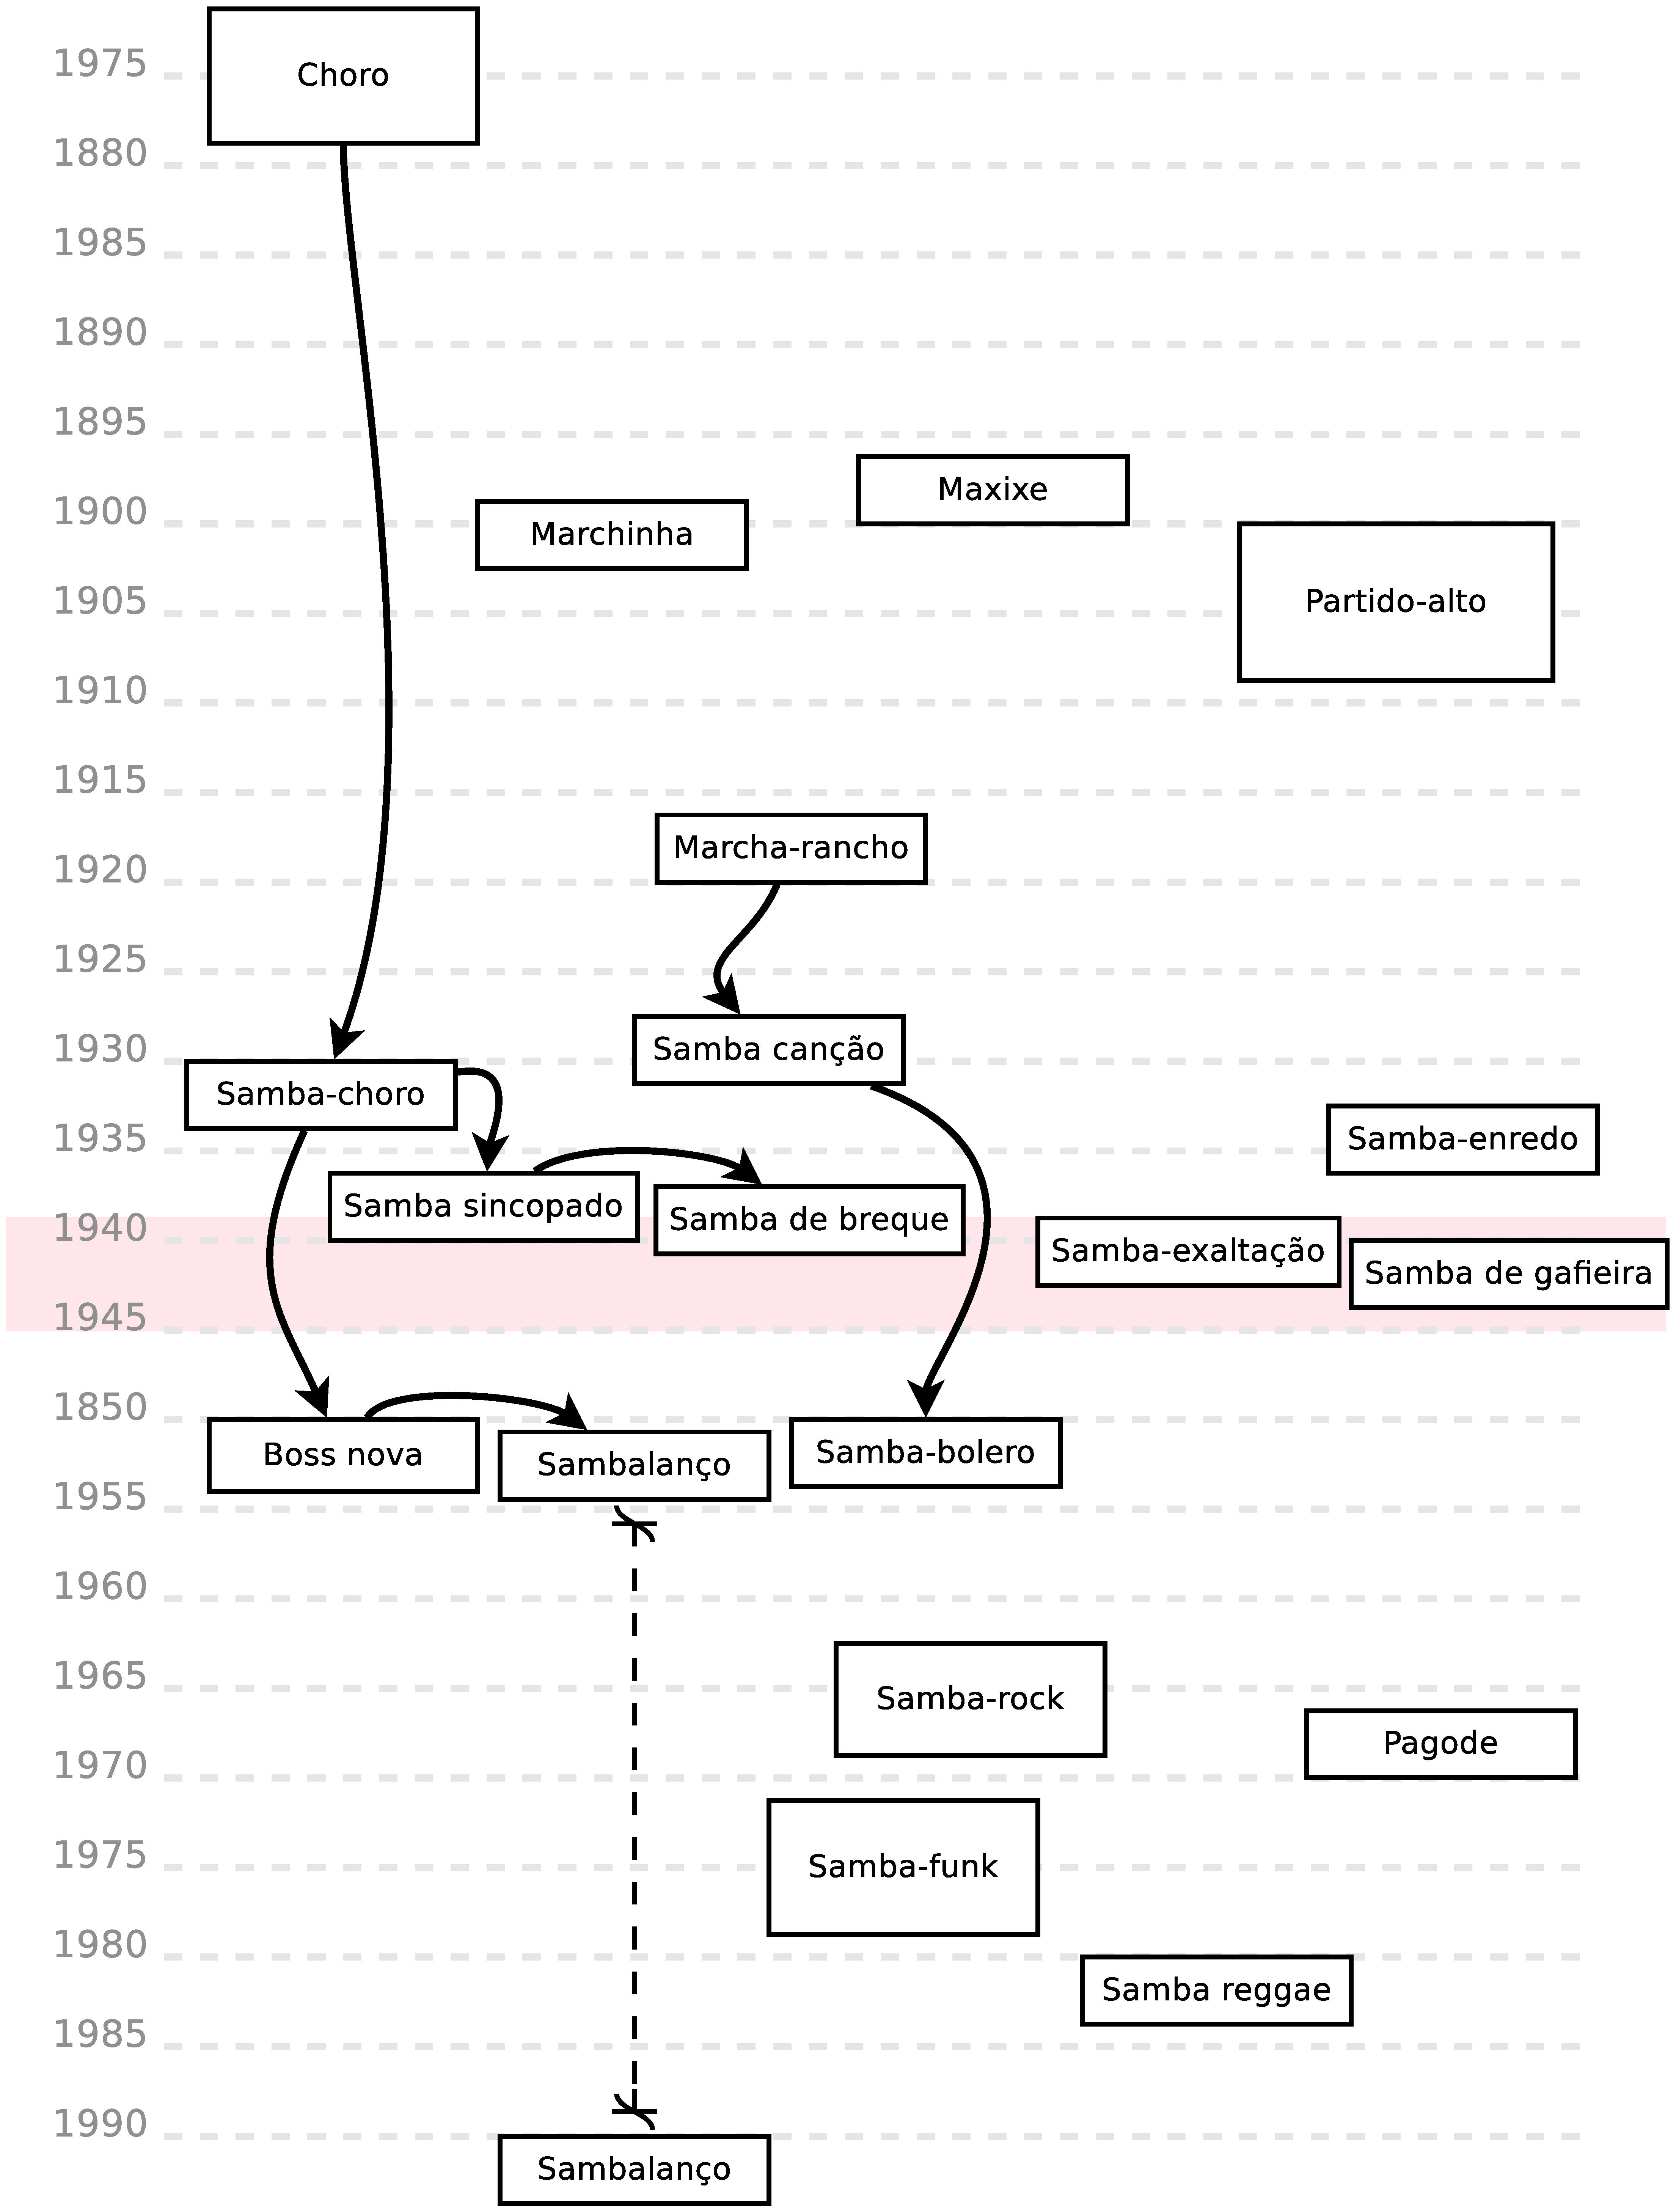
\includegraphics[width=0.95\textwidth]{chapters/cap-historia-musicasamba/musicatimeline.eps}
  \caption{Relação temporal entre os inícios dos subgêneros do samba.}
\label{fig:sambamusicatimeline1}
\end{figure}

%%%%%%%%%%%%%%%%%%%%%%%%%%%%%%%%%%%%%%%%%%%%%%%%%%%%%%%%%%%%%%%%%%%%%%%%%%%%%%%%
%%%%%%%%%%%%%%%%%%%%%%%%%%%%%%%%%%%%%%%%%%%%%%%%%%%%%%%%%%%%%%%%%%%%%%%%%%%%%%%%
\section{Que estilos de dança posso usar no samba (música)?}
\label{subsec:estilosdedanca}
A resposta mais simples poderia ser que, uma pessoa ao ser livre e independente,
pode escolher expressar-se na dança, de forma natural, como esta saia de si mesmo.
Porem, entrando em assuntos mais técnicos, 
e de acordo com os padrões socialmente mais comuns de ser achados atualmente;
existe um grupo de estilos de danças, que por suas caraterísticas, 
são consideradas que se enquadram muito bem na música de alguns subgêneros do samba.

Assim, nas seguintes seções, serão descritos alguns dos estilos de dança para a música do samba,  
que podemos achar nos salões e locais de dança no Brasil;
estes serão agrupados em estilos dançados em pares, e os que se dançam de forma separada. 


%%%%%%%%%%%%%%%%%%%%%%%%%%%%%%%%%%%%%%%%%%%%%%%%%%%%%%%%%%%%%%%%%%%%%%%%%%%%%%%%
\begin{comment}
\subsection{\textcolor{blue}{Estilos dançados em roda}}
\label{subsec:estilosdedancaroda}
Entre os estilos que se dançam em roda, temos:
\begin{description}
\item[Samba de roda:] Samba dançado em roda.
Para mais detalhes ir a página \pageref{ref:Samba-de-roda-danca}.

\item[Samba-de-umbigada:] 
São classificadas com este nome todas as danças que usem a umbigada na sua realização.
Para mais detalhes ir a página \pageref{ref:samba-de-umbigada}.

\item[Batuque (1900s):] Dança em roda onde se intercambiam os dançantes usando o gesto da umbigada.
Para mais detalhes ir a página \pageref{ref:batuquedanca}.

\item[Batucada:] Dança em roda onde se intercambiam os dançantes usando o gesto da pernada.
Para mais detalhes ir a página \pageref{ref:batucadadanca}.
\end{description}
\end{comment}
%%%%%%%%%%%%%%%%%%%%%%%%%%%%%%%%%%%%%%%%%%%%%%%%%%%%%%%%%%%%%%%%%%%%%%%%%%%%%%%%
\subsection{Estilos dançados em pares}
\label{subsec:estilosdedancapares}
Entre os estilos que se dançam a dois, existentes na atualidade, temos \cite[pp. 134]{perna2002samba}:
\begin{description}
\item[Samba de gafieira (dança):] 
\index{Dança!Samba de gafieira}
É uma dança a dois, que pode ser executada na maioria dos subgêneros do samba (música),
tendo exceções em: samba-enredo, samba reggae (música), samba rock (música), 
marcha, marcha-rancho e maxixe (música) \cite[pp. 134]{perna2002samba}.
No seus origens este tipo de dança era chamado de samba-batucada  \cite[pp. 134]{perna2002samba}. 
Para mais detalhes sobre o samba de gafieira, ver Seção \ref{subsec:gafieiradancaestilos}.

\item[Samba liso:] 
\index{Dança!Samba liso}
\index{Dança!Samba caminhado}
Atualmente se dança similarmente ao samba de gafieira, 
porem com um estilo mais elegante, sem ginga né passos de efeito, e dizer é uma dança mais ``lisa'';
se dança bem em : samba-canção, bossa nova e choro \cite[pp. 134]{perna2002samba}.

%%%%%%%%%%%%%%%%%%%%%%%%%%%%%%%
Podemos achar uma referencia interessante ao uso do termo \textbf{samba} e \textbf{liso}  no livro 
``Feitiço decente: Transformações do samba no Rio de Janeiro (1917-1933)'' (2001),
onde se pode intuir a procedência deste nome ou denominação, 
quando se faz referencia a um comentário de João da Baiana sobre o samba-de-umbigada e o samba de roda \cite[pp. 109]{sandroni2001feitico}: 
\begin{citando}
Nós tirávamos um verso e o pessoal sambava, um de cada vez ... 
Um saía para tirar o outro.
Se fosse a ``liso'' era só umbigada, mas se fosse para pegar ``duro'' já era capoiragem. 
\end{citando}
Pelo que no livro se comenta, que para o dançarino solista  escolher a seu sucessor podiam
existir duas modalidades, dependendo do tipo de roda, em ``samba liso'' (com umbigada) ou em ``samba duro'' 
(ou batucada\footnote{No qual a umbigada é substituída por uma pernada \cite[pp. 109]{sandroni2001feitico},
para mais detalhes ir a página \pageref{ref:batuquedanca}.}) \cite[pp. 109]{sandroni2001feitico}.
Esta referencia 
é particularmente interessante, pois como veremos na Seção \ref{cap:sambagafieira},
nos primórdios do samba nas gafieiras, existiam 3 formas em que esta era dançada: samba-canção (dança),
\textbf{samba-batucada} (dança)\footnote{Que 
é o nome com que era conhecido originalmente a atual samba de gafieira \cite[pp. 143]{perna2002samba}.} 
e \textbf{samba-liso} \cite[pp. 143]{perna2002samba};
estas duas últimas, não são as mesmas danças dos samba-de-umbigada, 
e sim novas formas de dançar o samba num ambiente mais civilizado como o salão de dança;
porem, estes nomes conservavam a mesma nomenclatura, na descrição 
da relativa relação à tosquedade dos movimentos.

%%%%%%%%%%%%%%%%%%%%%%%%%%%%%%%
Na ``Hemeroteca Digital Brasileira'' da Fundação Biblioteca Nacional,
não tem-se achado referencias\footnote{ Foram achadas,
2, 5, 3, 1 e 1 referencias brutas para as décadas de 1930, 1940, 1960, 1970 e 1980 respetivamente;
porem, estas não eram relativas ao samba liso de salão ou eram falsos acertos.} 
à frase ``\textbf{samba liso}'', nas décadas de 1930, 1940, 1960, 1970 e 1980;
as referencias achadas correspondem à década de 1950\footnote{Especificamente entre os anos 1950 e 1953.}  
com uma total de 327 referencias;
de todas estas, 326 correspondem à forte campanha 
de marketing do livro
``Como aprender a dançar'' , 
de Gino Forniciari. 
Por exemplo, podemos achar a primeira referencia em ``O Jornal'' (RJ),
do dia 17 de setembro de 1950, onde se pode ler \cite[3ra seção pp. 9]{jornalanunciodanca1}:
\begin{citando}
\begin{center}
Como aprender a dançar\\
4a edição ampliada
\end{center}
Com a nova dança, ``Baião'', \textbf{Samba liso}, e os
últimos passos de Bolero, Rumba, Swing, contendo
120 gráficos 330 passos, facilitando as senhoritas 
e cavalheiros a aprenderem em suas próprias 
casas em 10 dias apenas, no princípio sem
companheiro ou companheira. Método de ritmos modernos
pelo Prof. Gino Fornaciari, 
Diretor e Prof. do ``CURSO PRATICO DE DANÇAS RITZ''.
Aulas particulares, rua da Liberdade, 120.
Preço: Cr\$ 45,00 -- Pedidos pelo reembolso posta 
-- com o autor -- Caixa Postal, 649 -- SÃO PAULO 
\end{citando}
Todos estes anúncios vem na maioria das vesses acompanhados com um desenho como
o mostrado na Figura \ref{fig:desenholivrodanca1}, que indica todos os estilos de dança abordados no livro;
onde se diferencia entre dançar \textbf{samba} e \textbf{samba liso}.
\begin{figure}[h]
  \centering
    \includegraphics[width=0.5\textwidth]{chapters/cap-historia-musicasamba/comoaprenderdancar.jpg}
  \caption{Desenho da publicidade do livro ``Como aprender a dançar'' de Gino Forniciari,
publicado, no dia 17 de fevereiro de 1952, em ``Sport Ilustrado'' \cite[pp. 22]{sportlivropublidanca}.}
\label{fig:desenholivrodanca1}
\end{figure}



%%%%%%%%%%%%%%%%%%%%%%%%%%%%%%%
A outra referencia achada na ``Hemeroteca Digital Brasileira'' da Fundação Biblioteca Nacional,
apara a frase ``samba liso'', na década de 1950, foi a publicada o dia 26 de agosto de 1951,
no ``Diário do Nordeste'' de Caixas do Sul (RS), numa cronica de Walter Brugger da sua viagem por Europa,
num articulo titulado ``Genova! Primeiro Contato com a Europa!'',
onde se pode ler \cite[pp. 10]{nordestesambalisocronica}:
\begin{citando}
Ao nosso lado, numa área 
descoberta uma orquestra tocava para
quem quizesse dançar.
Repentinamente ouvimos uma melodia muito
nossa conhecida. Era o imortal ``Tico-Tico no Fubá''... Todavia,
apesar da melodia correta, o ritmo
era bastante falho. Continuando 
com os ritmos brasileiros, a orquestra 
tocou ainda ``Chiquita Bacana'',
mas em tempo de samba e ``Aquarela do Brasil''.
O que porém nos 
deixou mais atônitos foi o modo como 
era dançado o nosso samba. De 
brasileiro não tinha nada. Pelo que 
vimos, o \textbf{samba ``liso''} lhes é desconhecido 
e cada um procura ``requebrar'' o corpo mais que o outro,
mas de uma forma como nós só 
conhecemos no cinema mexicano. 
O meu amigo dava gostosas risadas e não era para menos,
ante a comicidade do espetáculo, tão 
impossível no Brasil quanto desconhecido para nós.
\end{citando}


%%%%%%%%%%%%%%%%%%%%%%%%%%%%%%%
Outra referencia ao \textbf{samba liso}, pode ser achada no livro ``Manual de Danças Gaúchas'' (1955)
onde se afirma que \cite[pp. 77]{cortesmanual}: 
\begin{citando}
A polquinha, como dança especifica, é executada por pares enlaçados,
mediante passos-de-marcha (É correograficamente  semelhante ao chamado 
\textbf{samba liso} ou \textbf{samba caminhado} dos salões urbanos).
\end{citando}


\item[Samba pagode:] 
\index{Dança!Samba pagode}
É um estilo de dança a dois, originário de São Paulo, 
é uma dança com poucos deslocamentos \cite[pp. 134]{perna2002samba}.
É um estilo de dança adaptado para ser dançado com o pagode paulista,
também chamado como Sambalanço\footnote{Ver página \pageref{ref:sambalanco}}.
%% https://www.youtube.com/watch?v=SfvoiXOGPn4
Ao igual que o sambalanço teve duas épocas com estilos musicais diferentes,
a dança \textbf{samba pagode}, sofreu também transformações acompanhando essas tendencias.
Podem-se observar atualmente 3 tipos de passo base: 
%% https://www.youtube.com/watch?v=rq1uhNXySds 
%% https://www.youtube.com/watch?v=SfvoiXOGPn4

O miudinho, que é um passo que se realiza abraçado com o par e de forma espelhada com este,
onde se executam 3 twist\footnote{É importante ter um sapato que deslise bem.} no lugar, 
só trocando de peso entre os pés, seguindo um ritmo, rápido-rápido-lento;
este movimento se executa simetricamente duas vesses para formar um ciclo completo,  
uma vez iniciando com o peso do corpo para o pé direito\footnote{Quando o primeiro twist é horário.} e a outra com o esquerdo.

O passo básico lateral, se realiza abraçado com o par  e de forma espelhada com este, 
é similar ao passo básico de capoeira,
ou a base aberta do forró\footnote{Só que aqui é abraçados.},
onde se produzem 3 movimento seguindo um ritmo, rápido-rápido-lento,
no primeiro momento, um pé vai para atrás, 
no segundo o outro ajeita sua posição deslocando-se levemente, 
procurando o centro e o equilíbrio do par dançante, e
no terceiro o pé que estava atrás volta ao lado do outro,
este movimento se executa simetricamente duas vesses para formar um ciclo completo,  
uma vez iniciando com pé direito e a outra com o esquerdo.
Este movimento é interessante para fazer deslocamento, 
que são realizados principalmente nesse primeiro movimento com o pé atrás, 
só que agora apontando para uma direção especifica.

A caidinha, se realiza abraçado com o par, 
este passo é similar ao picadilho (picadinho) de samba de gafieira,
porem com um deslocamento similar ao repique do forró;
no pagode paulista este movimento se executa seguindo um ritmo, rápido-rápido-lento,
onde o seguidor faz um movimento similar ao miudinho antes mencionado,
enquanto que o condutor tem uma liberdade criativa no 
seu movimento\footnote{O mesmo que acontece no picadilho de samba de gafieira.} 
enquanto respeite o ritmo, rápido-rápido-lento.


\item[Samba rock:] 
\index{Dança!Samba rock}
É um estilo de dança a dois, realizado nos bailes ``black'' paulistas desde a década de 1960, 
sendo esta uma dança variante das danças do swing/rock e parente do soltinho carioca \cite[pp. 135]{perna2002samba}.
se dança bem em: Swing, samba rock (música), samba com suingue e samba-funk \cite[pp. 135,138]{perna2002samba}.
O samba rock se dança de mão dadas, e se carateriza por ter muitas voltas,
executadas na maior parte de vesses pelas  seguidores;
porem, é uma dança estacionaria pois os dançantes rara vez se deslocam pelo salão, 
e pelo contrario ficam trabalhando seus passos num mesmo lugar  \cite[pp. 135,138]{perna2002samba}.
Quando um espectador externo vê esta dança perceberá muitas figuras usando só os braços,
com enrosques, voltas, enlaces, etc.
Enquanto os pés de ambos dançarinos fazem uma mesma marcação, num constante e repetitivo rápido-rápido-lento,
caminhando unicamente sobre um circulo imaginário no chão, uma vez em sentido horário e outra em anti-horário.

\item[Samba funkeado:] 
\index{Dança!Samba funkeado}
Também é chamado de estilo Jimmy de Oliveira ou simplesmente  samba Jimmy, 
em aluição a seu criador.
Este estilo de dança a dois foi criado no ano de 1998.
Com muito esforço Jimmy, num período aproximado de 6 meses, 
criou a estrutura da dança, desde iniciante ate avançado;
no ano de 1999 ele  chamou a esse estilo como ``samba quebrado'';  
posteriormente renomeou  para ``samba Jimmy'', 
recebeu algumas criticas e no ano 2001 decidiu renomeá-lo para ``samba funk'',
porem isto trouxe confusões   ao ser associado com a música funk, existente em Rio de Janeiro,
muito distante da proposta dele, e
finalmente a meados do 2005 ele decidiu chamá-lo ``samba funkeado''  \cite{sambafunkeadoJimmyDeOliveiraPart1}.
A Figura \ref{fig:funkeadocrono1} mostra a cronologia de nomes para este estilo.
\begin{figure}[h]
  \centering
    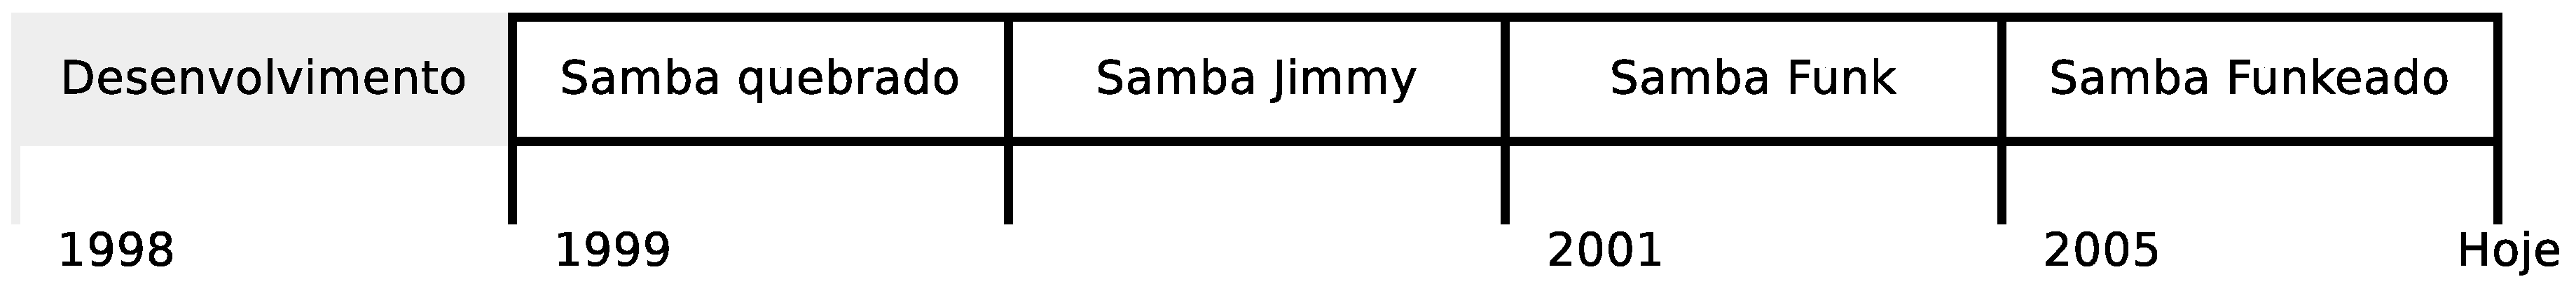
\includegraphics[width=0.85\textwidth]{chapters/cap-historia-musicasamba/sambafunkeado.eps}
  \caption{Cronologia dos nomes para samba funkeado.}
\label{fig:funkeadocrono1}
\end{figure}

O estilo foi criado para, em palavras de Jimmy: ``contribuir em função da música'', 
numa tentativa de agregar movimento em coerência como as músicas que ele gostava;
sendo estas interpretadas por:
Djavan, Jorge Ben Jor, Tim Maia, Leny Andrade \cite{sambafunkeadoJimmyDeOliveiraPart1}, que em seu momento, 
presentaram músicas de bossa nova ou que eram influenciadas pelo jazz, funk norte-americano ou ``black music'' \cite{sambafunkeadoJimmyDeOliveiraPart1} \cite{sambafunkeadoJimmyDeOliveiraPart3},
Jimmy indica que seu estilo procura ir em função da música escutada no brasil, 
e que a maioria da música atual é influenciada pelo funk norte-americano;
como a música de: João Sabiá. 

O samba funkeado pode ser dançado em gêneros como ``black music'',
em pagodes funkeados (Sorriso maroto, Netinho de Paula, pixote, etc.), em sambas com influencia do jazz \cite{sambafunkeadoJimmyDeOliveiraPart3}, etc. 

O samba funkeado tem 3 tendencias ou estruturas  \cite{sambafunkeadoJimmyDeOliveiraPart2}:
\begin{itemize}
\item \textbf{Samba funkeado}, primigênio.
\item \textbf{Samba funkeado fragmentado}; exemplo: um movimento que é de sentar, que gastaria um tempo, 
passa a ter ate 3 tempos; é dizer, fragmenta os movimentos. 
O fragmentado também permite dançar com movimentações em contrapeso no par de dança.
\item \textbf{Samba funkeado samsurf}, com uma postura mais curvada.
\end{itemize}

%e em seu ídolo Michael Jackson \cite{sambafunkeadoJimmyDeOliveira2}.
 

\item[Samba internacional:] 
\index{Dança!Samba internacional}
É um estilo de dança a dois, influenciado pelo maxixe;
se dança principalmente fora do Brasil e existem basicamente dois estilos: 
o estilo internacional e o estilo norte-americano (EE.UU.) \cite[pp. 134-135]{perna2002samba}.

O samba introduzida a EE.UU. é uma dança de salão muito animada, 
com música de ritmo alegre, que sugere um estilo de movimento que pode
chegar a ser tão turbulento quanto os movimentos do Jive.
O padrão de passos básicos é similar aos achados no Fox-Trot e o Waltz,
sendo estes: fwd-swd-close ... bwd-swd-close; e
tem passos com tempos que seguem uma sequência: 
quick-quick-slow\footnote{Rápido-rápido-lento.} ... quick-quick-slow \cite{parson2016ballroom}.

Observando os campeonatos internacionais onde este estilo é usado, 
se percebe que o samba internacional é dançado em qualquer estilo musical que
tenha sotaque ou de a impressão de ter raiz afro-latina.

\end{description}~

A Figura \ref{fig:sambadavavsmusica} mostra as relações entre os estilos de dança a dois atuais,
 e os subgêneros do samba \cite[pp. 134-138]{perna2002samba}.

\begin{figure}[h]
  \centering
    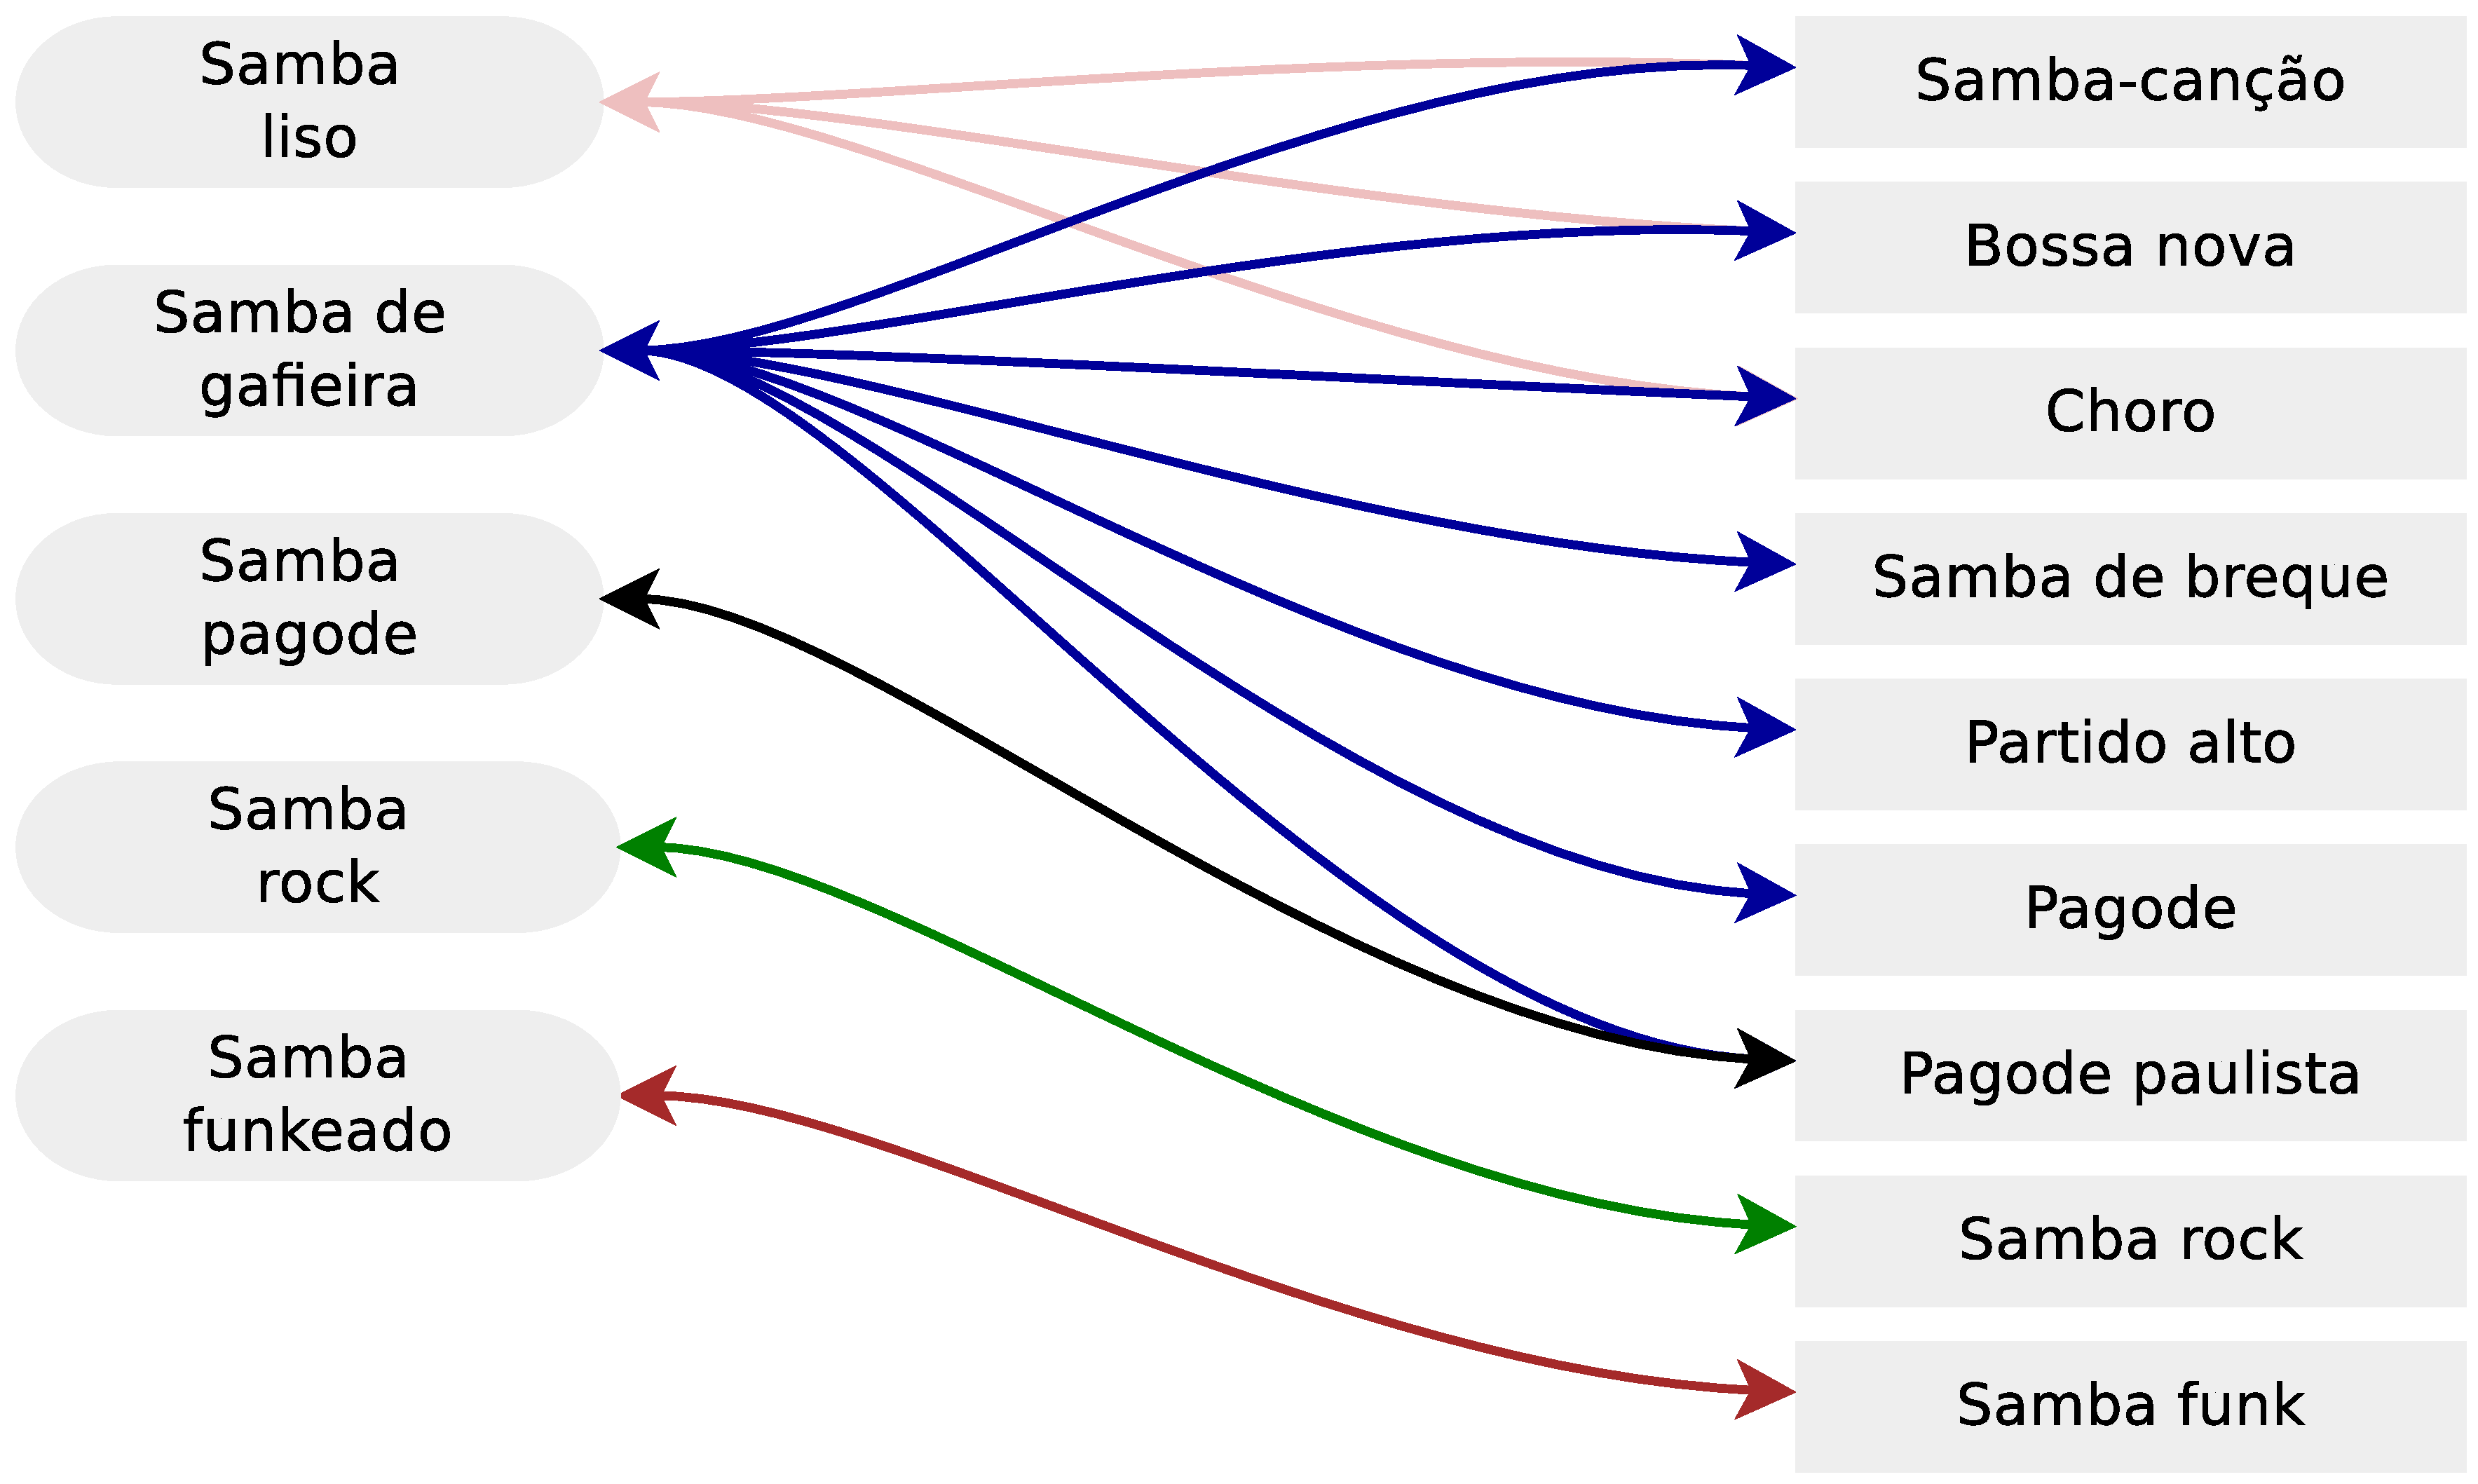
\includegraphics[width=0.6\textwidth]{chapters/cap-historia-musicasamba/dancavcmusica.eps}
  \caption{Relações entre os estilos de dança a dois e os subgêneros do samba.}
\label{fig:sambadavavsmusica}
\end{figure}

%%%%%%%%%%%%%%%%%%%%%%%%%%%%%%%%%%%%%%%%%%%%%%%%%%%%%%%%%%%%%%%%%%%%%%%%%%%%%%%%
\subsection{Estilos dançados individualmente ou separados }
Entre os estilos que se dançam de forma separada temos \cite[pp. 134]{perna2002samba}:
\begin{description}
\item[Samba reggae  (dança):] Este estilo de samba que se dança separado, 
é uma dança baiana também conhecida como axé-dance, samba baiano ou pagode baiano,
se dança em samba reggae (música) \cite[pp. 134]{perna2002samba}.

\item[Samba no pé:] É o estilo usado nas quadras das escolas de samba,
se dança bem em estilos musicais como: 
samba enredo ou em qualquer samba rápido  \cite[pp. 134]{perna2002samba}.

\item[Marcha de carnaval:] É uma dança própria do carnaval para se dançar em cordões.
se dança bem em: marchas, marchas-rancho e samba-enredo lentos  \cite[pp. 135]{perna2002samba}.

\end{description}
~

A Figura \ref{fig:sambadavavsmusicaseparado} mostra as relações existentes, 
entre os estilos de dança que se dançam separados e alguns subgêneros do samba  \cite[pp. 134-138]{perna2002samba}.

\begin{figure}[h]
  \centering
    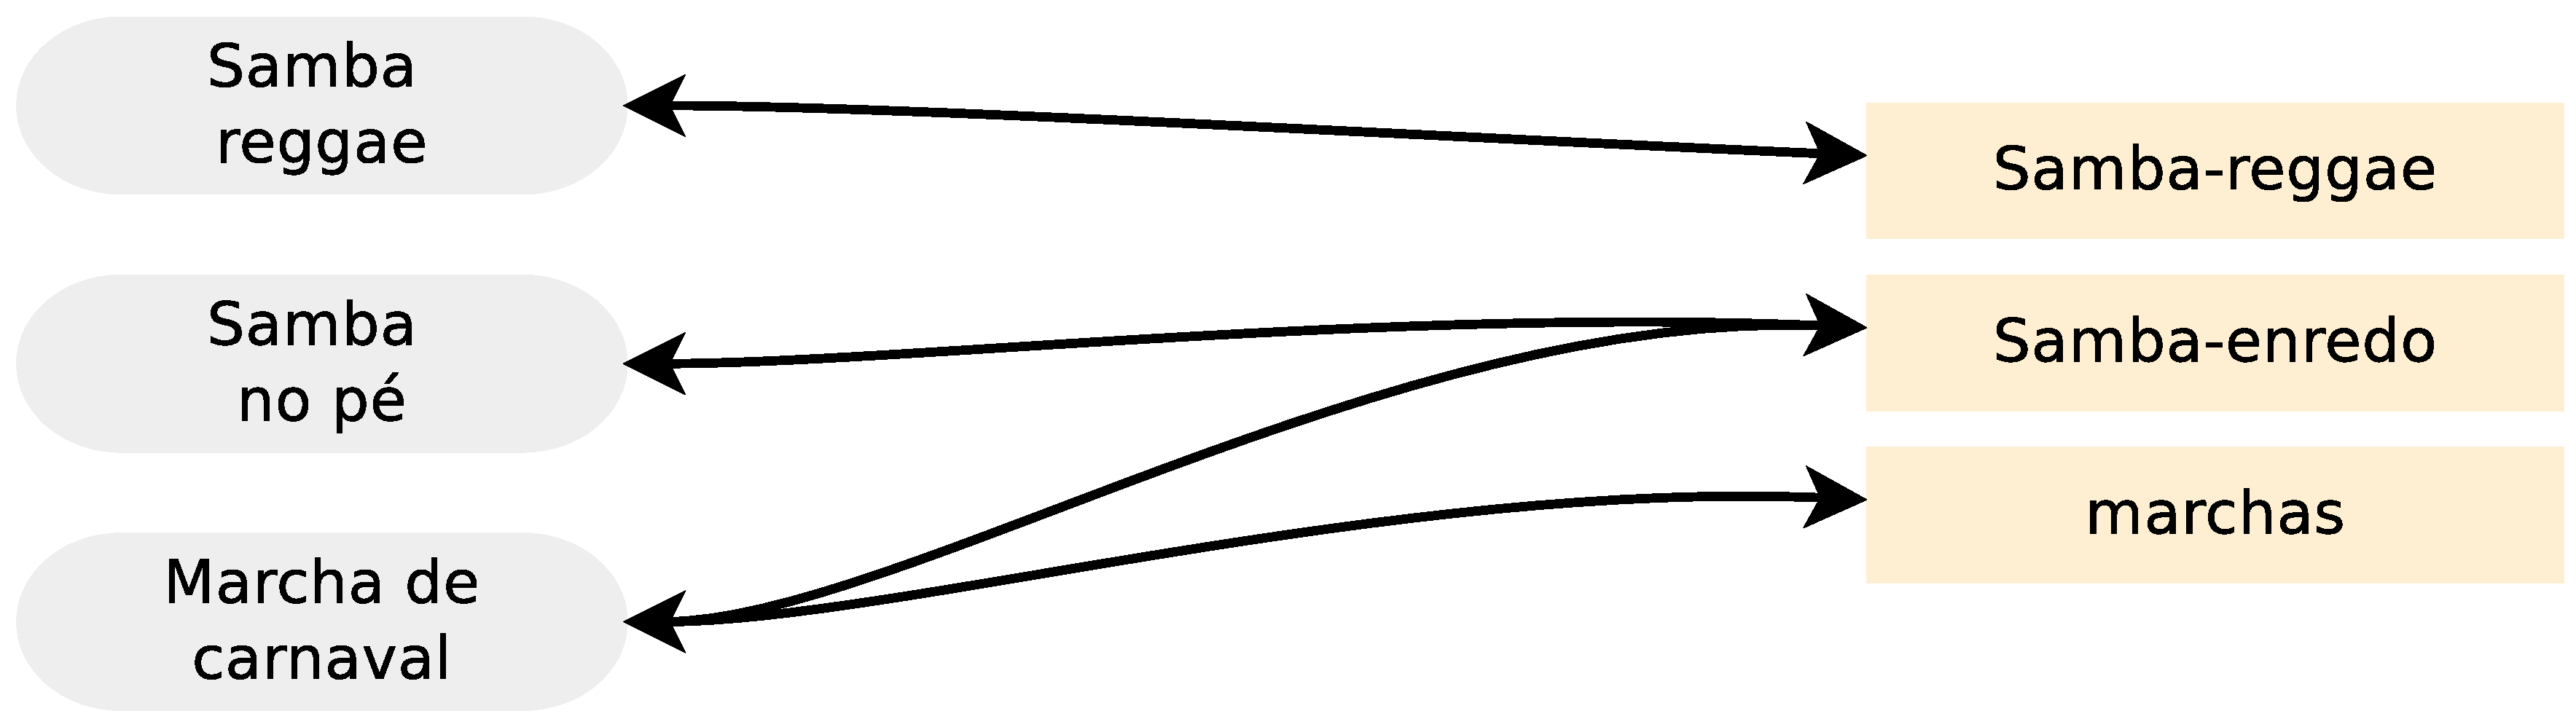
\includegraphics[width=0.6\textwidth]{chapters/cap-historia-musicasamba/dancavcmusicaseparado.eps}
  \caption{Relações entre os estilos de dança (separados) e os subgêneros do samba.}
\label{fig:sambadavavsmusicaseparado}
\end{figure}


%%%%%%%%%%%%%%%%%%%%%%%%%%%%%%%%%%%%%%%%%%%%%%%%%%%%%%%%%%%%%%%%%%%%%%%%%%%%%%%%
%% CAPITULO
%%%%%%%%%%%%%%%%%%%%%%%%%%%%%%%%%%%%%%%%%%%%%%%%%%%%%%%%%%%%%%%%%%%%%%%%%%%%%%%%
\chapterimage{chapter_head_2.pdf} % Chapter heading image

\chapter{\textcolor{green}{Historia do samba de gafieira  (dança)}}
\label{cap:sambagafieira}
\index{Dança!Samba de gafieira}


\section{Lundum (a dança do lundu)} 
\label{sec:lundu}
\index{Dança!Lundu}
O lundum é o estilo de dança que lhe corresponde ao gênero musical lundu \cite[pp. 18]{perna2002samba}.
Esta é uma dança, brasileira, de roda e umbigada; e teve sua origem no batuque dos bantos africanos,
e provavelmente foi trazida de Angola pelos escravos na segunda metade do século XVIII \cite[pp. 48]{tinhorao1986pequena} \cite[pp. 188]{dourado2004dicionario},
sendo que as primeiras referencias conhecidas se remontam a 1780 
descrevendo a dança como indecente e licenciosa \cite[pp. 51]{tinhorao1986pequena} \cite[pp. 19]{perna2002samba}.
Posteriormente foi introduzida aos salões das cortes do Brasil e Portugal, 
dançado elegantemente nas cortes, porem indecentemente pela gente comum   \cite[pp. 19]{perna2002samba} \cite[pp. 188]{dourado2004dicionario}.
No Brasil esta dança teve influencias da ``Modinha''(Portuguesa) e do ``Fandango''(Espanhol) \cite[pp. 188]{dourado2004dicionario}.

A partir de 1820 o lundum é apresentado, como dança de caráter libidinoso nos teatros de Baia, Pernambuco e Rio de Janeiro;
onde eram representados pequenos quadros cômicos, 
mostrando a umbigada e outras caraterísticas da dança \cite[pp. 19]{perna2002samba}.


\section{Maxixe (dança)}
\label{sec:maxixe}
\index{Dança!Maxixe}
Esta é uma dança urbana afro-brasileira \cite[pp. 4]{musicasambavariasdef1}, 
em compasso binário, surgida em Rio de Janeiro, 
na Cidade Nova e nos cabarés de Lapa \cite[pp. 465]{marcondes1977enciclopedia}  \cite[pp. 198]{dourado2004dicionario}, 
aproximadamente entre 1870 e 1880 \cite[pp. 58]{tinhorao1986pequena} \cite[pp. 465]{marcondes1977enciclopedia}  \cite[pp. 62]{reinato2010musica}.

A dança era considerada de baixe ralé pela sociedade local, 
pois era entendida como um modismo indecente das classes baixas, imoral como o Lundu \cite[pp. 198]{dourado2004dicionario}.
Esta dança recebeu influencias da polca \cite[pp. 198]{dourado2004dicionario} e 
da Habanera \cite[pp. 62]{reinato2010musica}.


O maxixe tinha uma boa quantidade de passos como: 
\begin{itemize} 
\item parafuso  \cite[pp. 68, 93, 129]{efege1974maxixe} \cite[pp. 465]{marcondes1977enciclopedia} \cite[pp. 62]{tinhorao1986pequena}, 
\item janela  \cite[pp. 129]{efege1974maxixe},
\item jocotó \cite[pp. 83, 96, 173]{efege1974maxixe},
\item saca-rolha \cite[pp. 465]{marcondes1977enciclopedia}, 
\item balão \cite[pp. 93]{efege1974maxixe} \cite[pp. 465]{marcondes1977enciclopedia}, 
\item balão apagado \cite[pp. 68]{efege1974maxixe} \cite[aproximadamente min. 11:35]{MaxixeDocumentario1},
\item balão caindo  \cite[pp. 129, 131]{efege1974maxixe} \cite[pp. 62]{tinhorao1986pequena},
\item corta-jaca  \cite[pp. 131]{efege1974maxixe},
\item urubu malandro  \cite[pp. 131]{efege1974maxixe},
\item sino \cite[pp. 68]{efege1974maxixe}, 
\item carrapeta  \cite[pp. 465]{marcondes1977enciclopedia}, 
\item corta-capim \cite[pp. 465]{marcondes1977enciclopedia} \cite[pp. 62]{tinhorao1986pequena}, 
\item cobrinha \cite[pp. 62]{tinhorao1986pequena},
\item maxixe puladinho \cite[pp. 177]{1920revista},
\item etc. 
\end{itemize}
Num principio o maxixe era dançado nas músicas de tango, havanera, polca e lundu; 
e só foi ate o final do século XIX que ganhou uma música com gênero próprio \cite[pp. 465]{marcondes1977enciclopedia},
criado pela fusão da polca, o schottisch e a mazurca \cite[pp. 58]{tinhorao1986pequena}.

No inícios do século XX o maxixe foi exportado e dançado na Europa, atingindo um grande sucesso, 
chegando a ser apresentado pelo dançarino ``Duque'' em Paris (1914) e em Londres (1922) \cite[pp. 465]{marcondes1977enciclopedia}.
Este dançarino é considerado o civilizador do maxixe \cite[pp. 129]{efege1974maxixe}.

Uma explicação muito interessante do maxixe é cantada pela atriz, Aurélia Delorme,
numa representação num quadro de revista, interpretando  ``Maxixe Aristocrático'' (1904, José Nunes), 
que arrancava aplausos e provocava pedidos de bis;
o seguinte texto indica sua pauta \cite[pp. 80-81]{efege1974maxixe} \cite{REIS2003}: 
\begin{citando}
O maxixe tem ciência,\\
ou pelo menos tem arte.\\
Para haver proficiência\\
basta mexer certa parte.\\
Pois o próprio Padre Santo,\\
sabendo o gosto que tem,\\
virá de Roma ao Brasil\\
dançar maxixe também.\\ 
\end{citando}



\section{\textcolor{green}{Samba de gafieira (dança)}}
\index{Dança!Samba de gafieira}
O samba de gafieira, como dança, descende principalmente do maxixe (dança),
que a sua vez foi gerado  pela união do  lundu, 
a polca e outras danças europeias.
Assim, misturando o maxixe com a ginga, e o ritmo de outras danças africanas, 
é que se obteve o que agora chamaríamos como samba de gafieira (primigênio)\footnote{
Primitivo; primordial; o primeiro da sua espécie. = PRIMÍGENO \cite{priberamprimigenio}.
} \cite[pp. 139]{perna2002samba}.




A Figura \ref{fig:formuladosambagafieira} mostra a árvore genealógico do samba de gafieira (primigênio),
visto quando o samba fez sua aparição nos salões de dança denominados gafieiras.
\begin{figure}[h]
  \centering
  \begin{subfigure}[b]{0.535\textwidth}
    \centering
    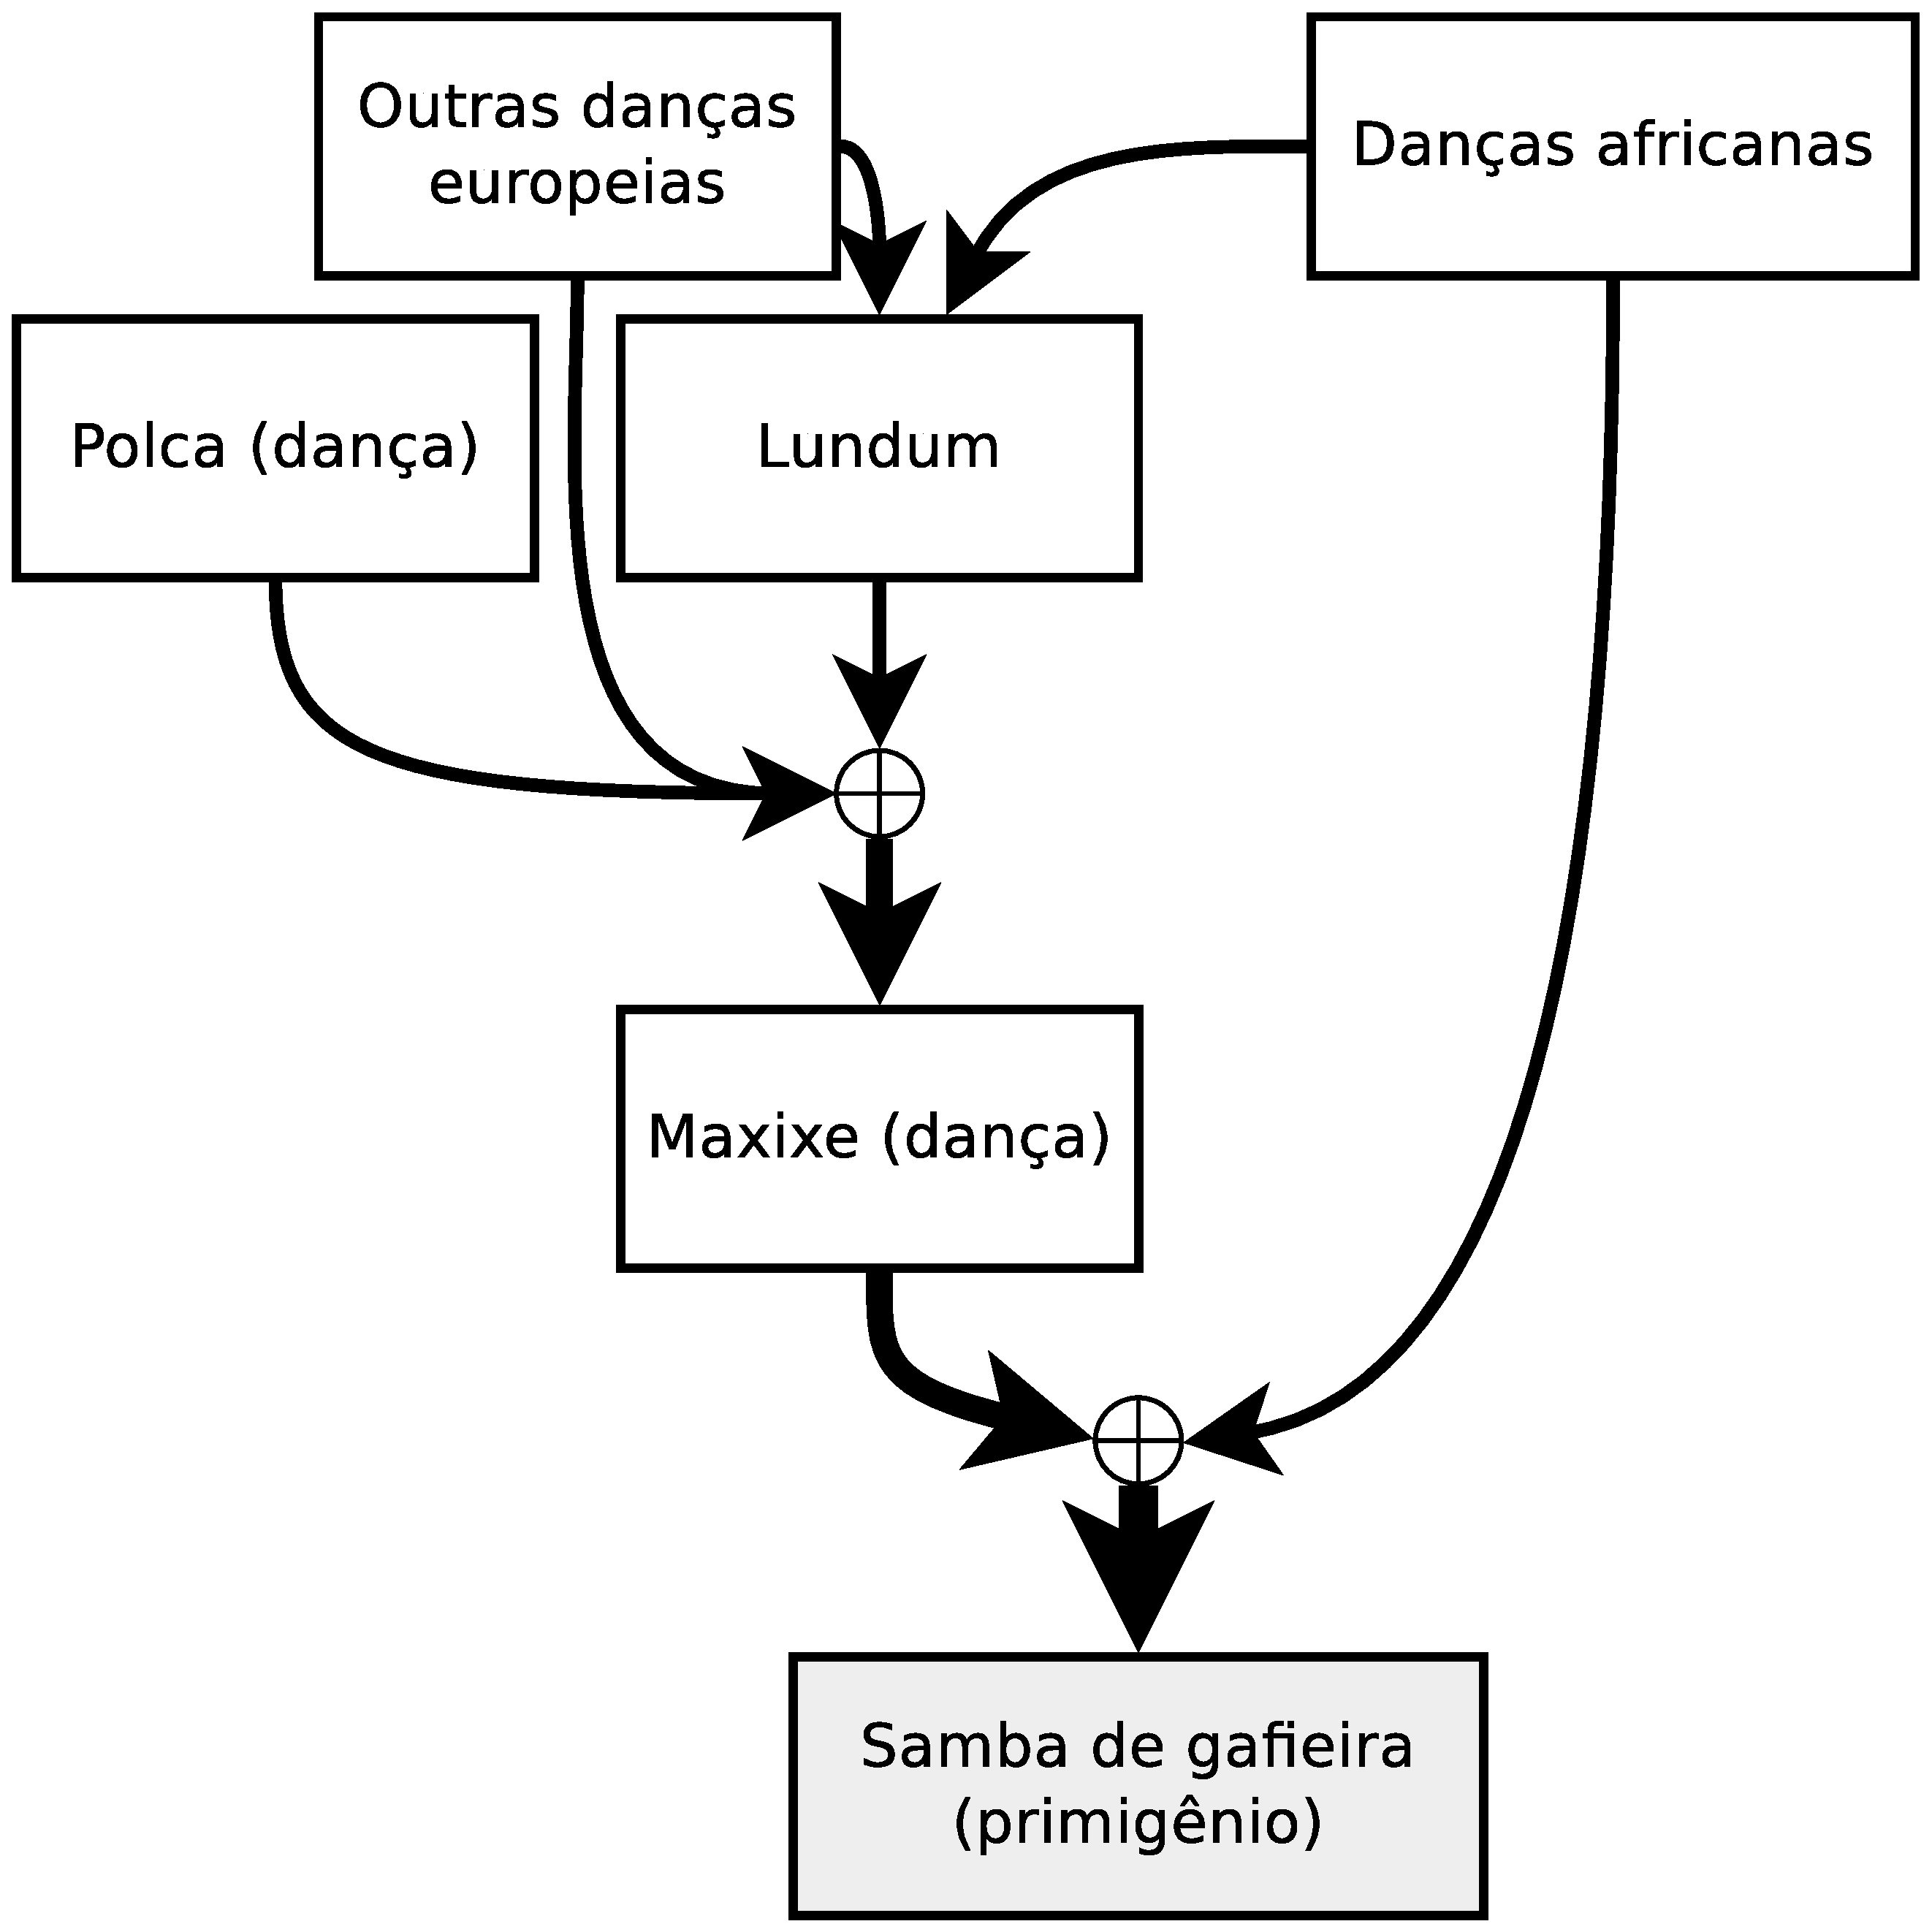
\includegraphics[width=\textwidth]{chapters/cap-historia-sambagafieira/sambagafieiraformula.eps}
    \caption{Formação do samba de gafieira (primigênio).}
    \label{fig:formuladosambagafieira}
  \end{subfigure}
  \begin{subfigure}[b]{0.385\textwidth}
    \centering
    \includegraphics[width=\textwidth]{chapters/cap-historia-sambagafieira/sambagafieiraformula2.eps}
    \caption{Formação do samba de gafieira (atual).}
    \label{fig:formuladosambagafieira2}
  \end{subfigure}
\caption{Formula da criação do samba de gafieira.}
\label{fig:formuladosambagafieiraall}
\end{figure}


O aparecimento do samba nos salões de dança, 
foi um grande impacto para as pessoas que frequentavam estes lugares;
sendo considerado um ritmo novo e ligeiro,
que desagradou aos bailarinos de maior idade e menos ágeis \cite[pp. 6 - cad. B]{entrevistajuliojournalbrasil1}.
O senhor, Júlio Simões, Administrador da ``Kananga do Japão'' e posteriormente socio
do ``Elite Club'', chegou a temer pelo futuro do seus empreendimentos; porem, para sorte dele, 
o samba fez muito sucesso no Elite,
e passou a ser considerado vestibular indispensável para qualquer pessoa que pretendesse ser bailarino, 
compositor ou instrumentista \cite[pp. 6 - cad. B]{entrevistajuliojournalbrasil1}.

\PRLsep{Samba nos salões em 1940}

Pode-se estabelecer o ingresso do samba, aos salões de dança, entre os anos de 1930 e 1940 \cite[pp. 140]{perna2002samba}.
Em palavras do Prof. de dança Gino Fornaciari, 
o samba dessa época tinha um aprecido com o Foxtrot e a Rumba, se dançava num compasso binario,
sendo esta dança a preferida do mulato brasileiro
%sendo este estilo de dança de salão que nasceu na \hyperref[ref:batucadadanca]{\textbf{batucada}} 
%de pretos que descia à cidade na epoca das festas 
\cite[pp. 50]{fornaciari1947aprender}.
Para a decada de 1940 o samba carioca de salão \cite[pp. 50]{fornaciari1947aprender},  já tinha ganhado muita força nos salões,
e podia-se ver 3 modalidades de dançar o samba \cite[pp. 58]{freitas1959danca} \cite[pp. 142-143]{perna2002samba} 
\cite[pp. 51]{fornaciari1947aprender}:
\begin{itemize}
\item \textbf{Samba-canção (dança)},
\index{Dança!Samba-canção} 
Era uma dança com balanços aos lados que se executava de joelhos flexionados,
usando dois movimentos por cada compasso binario \cite[pp. 58]{freitas1959danca} 
\cite[pp. 51]{fornaciari1947aprender} \cite[pp. 143]{perna2002samba}; 
na atualidade é um modo de dança extinto \cite[pp. 143]{perna2002samba}.

Sobre os passos usados entre 1947-1959, 
na Figura \ref{fig:samba-cancao-basico-frente} se mostra o passo básico para a frente do samba-canção,
e na  Figura \ref{fig:samba-cancao-basico-frente} o mesmo movimento para trás;
em ambos casos se usa os 2 movimentos antes mencionados, e a cor cinza indica a posição inicial \cite[pp. 51]{fornaciari1947aprender} \cite[pp. 59-60]{freitas1959danca}. 
\begin{figure}[h]
    \centering
    \begin{subfigure}[b]{0.4\textwidth}
        \centering
        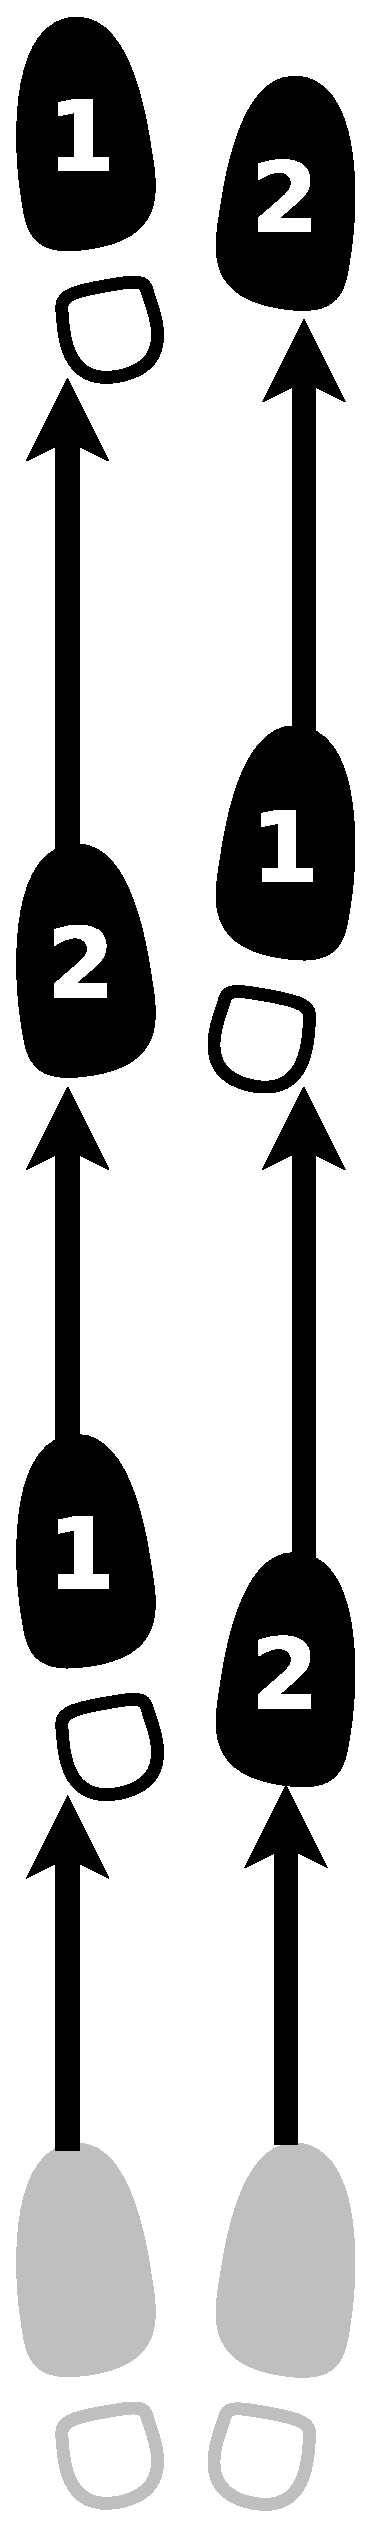
\includegraphics[width=0.25\textwidth]{chapters/cap-historia-sambagafieira/samba-cancao-basico-frente.eps}
        \caption{Passo básico para a frente.}
        \label{fig:samba-cancao-basico-frente}
    \end{subfigure}
    ~ %add desired spacing between images, e. g. ~, \quad, \qquad, \hfill etc. 
      %(or a blank line to force the subfigure onto a new line)
    \begin{subfigure}[b]{0.4\textwidth}
        \centering
	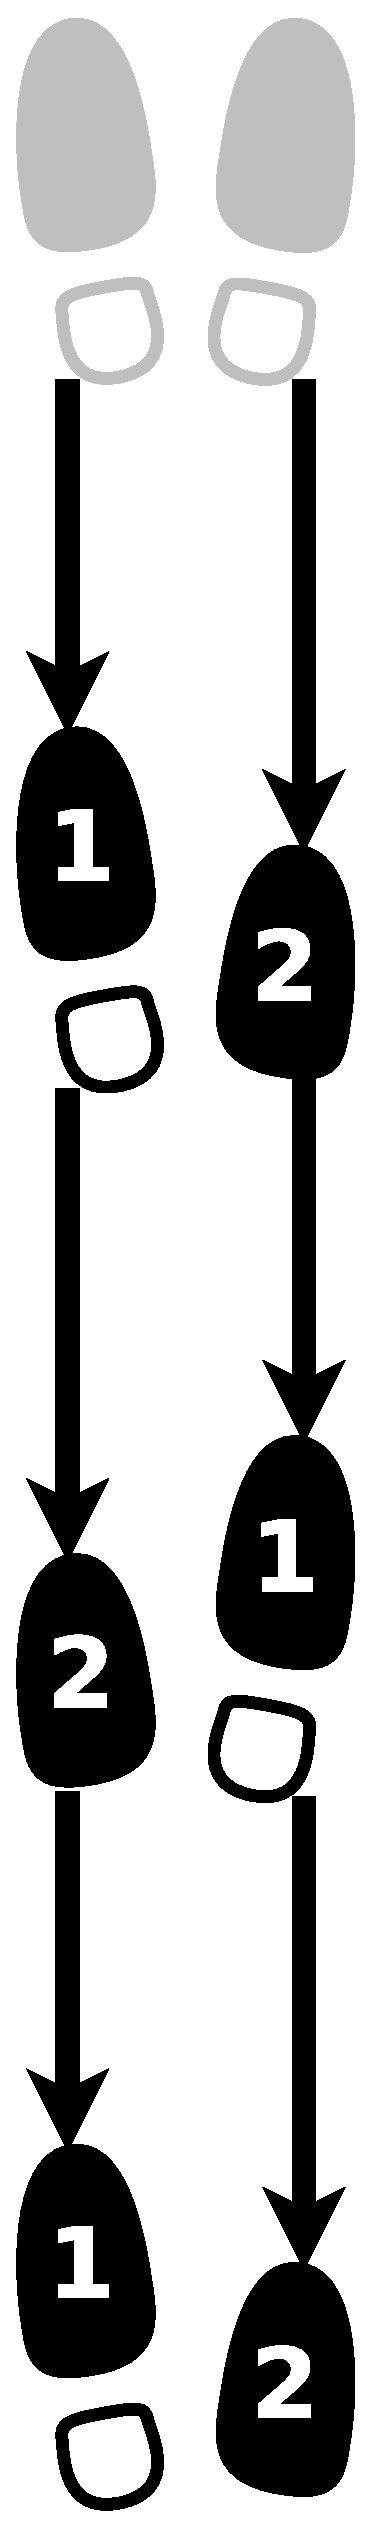
\includegraphics[width=0.25\textwidth]{chapters/cap-historia-sambagafieira/samba-cancao-basico-tras.eps}
        \caption{Passo básico para trás.}
        \label{fig:samba-cancao-basico-tras}
    \end{subfigure}
    \caption{Samba-canção da década de 1959.}\label{fig:samba-cancao-basico}
\end{figure}


\item \textbf{Samba-batucada},
\index{Dança!Samba-batucada} 

O samba-batucada é o samba de gafieira (primigênio) \cite[pp. 143]{perna2002samba}.

Existe uma menção sobre este estilo no ``Jornal do Brasil'', no dia 9 de janeiro de 1938,
onde se indica \cite[pp. 4]{musicasambavariasdef1}:
\begin{citando}%%
Tentativas isoladas de puro 
snobismo e ás vezes de compreensão 
inexata da origem da 
musica e dansa, chamam-no de samba jongo, \textbf{samba batucada} ou
pretendem mistura-lo com o fox, -- samba fox ou com a rumba samba-rumba.
\end{citando}



No livro ``Feitiço decente: Transformações do samba no Rio de Janeiro (1917-1933)'' (2001),
se comenta, sobre uma roda do samba, que para o dançarino solista  escolher a seu sucessor podiam
existir duas modalidades, em ``samba liso'' (com umbigada) ou em ``samba duro'' 
(ou batucada) no qual a umbigada é substituída por uma pernada \cite[pp. 109]{sandroni2001feitico}.
Deste comentário pode ser deduzido de onde vem a denominação \textbf{samba-batucada}, 
que surgiu nos salões de dança apos 1930; pois já existia uma tradição na nomenclatura,
em separar duas formas de dançar uma mais leve (a liso) e uma mais brusca (batucada);
assim, a variante de samba no salão que tendia a explorar movimentos muito  gingados, bruscos ou rápidos,
foi nomeado de samba-batucada, em contraposição ao samba liso onde né se flexionavam os joelhos pra dançar.  



O samba-batucada era, entre 1947 e 1959, uma dança com balanços que se dançava de joelhos flexionados  
e usava 3 movimentos por compasso, que exigia uma maior rapidez, 
especialmente no terceiro movimento que é mais rápido e curto \cite[pp. 61]{fornaciari1947aprender} \cite[pp. 58,66]{freitas1959danca};
seguindo essa descrição, 
o mais provável é que se dançara seguindo uma distribuição de tempos,
parecida ao ritmo do baião de 1949 \cite{CORTES2014}, como pode-se ver na Figura \ref{time:sambabatucada}.
\begin{figure}[H]
\centering
\begin{abc}[name=abc-sambabatucada]
X: 1 % start of header
K: C stafflines=1 % scale: C major
M: 2/4 %meter - compasso
%Q:1/4=100
V:1 clef=perc stem=up %name="TC"   sname="TC"
[V:1] |:  B3/2 B/2 B1 z1 | B3/2 B/2 B1 z1 | B3/2 B/2 B1 z1 | B3/2 B/2 B1 z1 :|
w:        P1   P2  P3      P1   P2  P3      P1   P2  P3      P1   P2  P3
\end{abc}
\caption{Frase de 8 tempos onde P1, P2 e P3 indicam o pé 1, 2 e 3 respetivamente.}
\label{time:sambabatucada}
\end{figure}

Sobre os passos usados na época, 
na Figura \ref{fig:samba-batucada-basico-frente} se mostra o passo básico para a frente do samba-batucada,
e na  Figura \ref{fig:samba-batucada-basico-tras} o mesmo movimento para trás;
em ambos casos se usa os 3 movimentos antes mencionados, e a cor cinza indica a posição inicial \cite[pp. 61-62]{fornaciari1947aprender} \cite[pp. 63]{freitas1959danca}. 
\begin{figure}[h]
    \centering
    \begin{subfigure}[b]{0.4\textwidth}
        \centering
        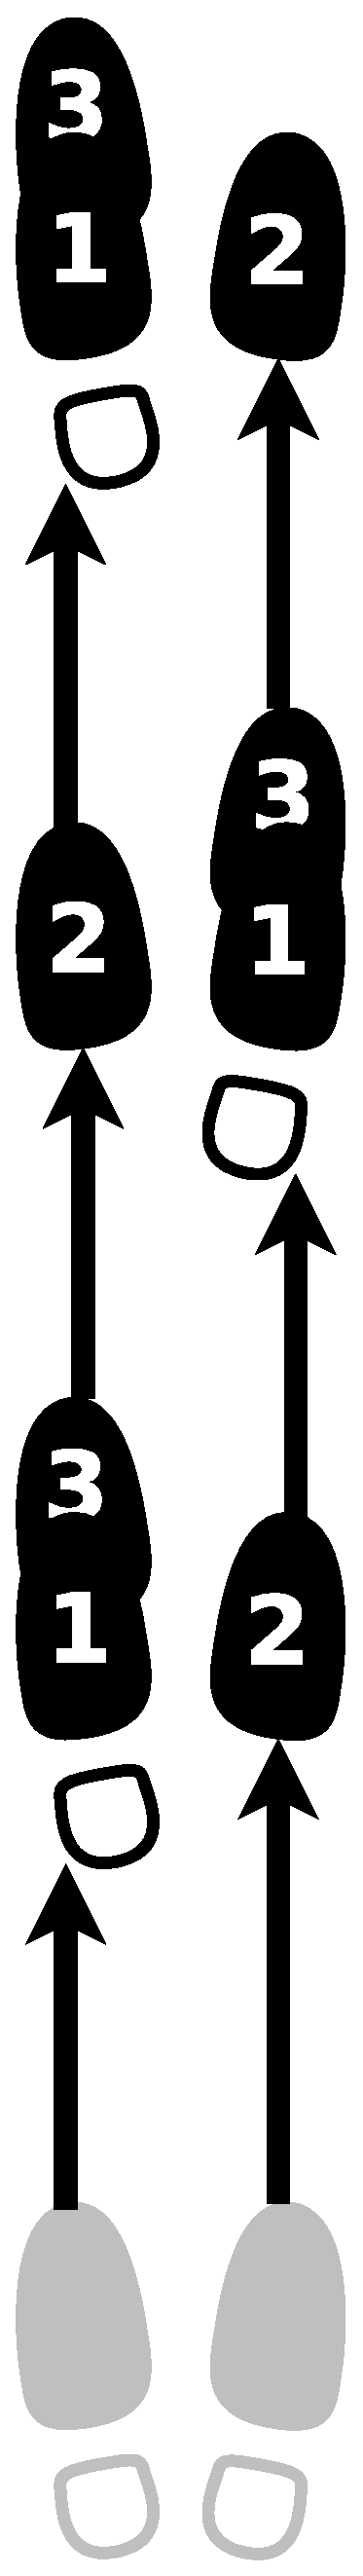
\includegraphics[width=0.25\textwidth]{chapters/cap-historia-sambagafieira/samba-batucada-basico-frente.eps}
        \caption{Passo básico para a frente.}
        \label{fig:samba-batucada-basico-frente}
    \end{subfigure}
    ~ %add desired spacing between images, e. g. ~, \quad, \qquad, \hfill etc. 
      %(or a blank line to force the subfigure onto a new line)
    \begin{subfigure}[b]{0.4\textwidth}
        \centering
	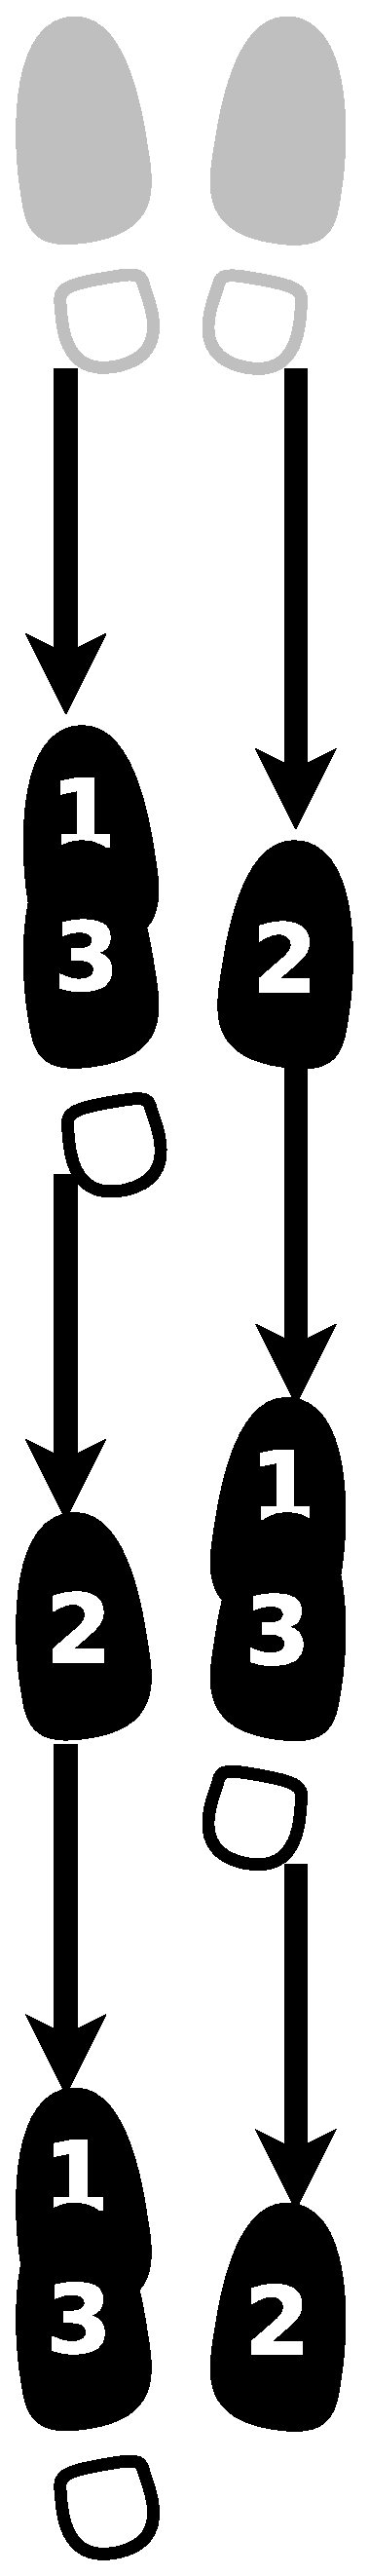
\includegraphics[width=0.25\textwidth]{chapters/cap-historia-sambagafieira/samba-batucada-basico-tras.eps}
        \caption{Passo básico para trás.}
        \label{fig:samba-batucada-basico-tras}
    \end{subfigure}
    \caption{Samba-batucada da década de 1959.}\label{fig:samba-batucada-basico}
\end{figure}

Outros passos conhecidos no ano de 1947, para este estilo de samba, tem nomes como: 
o pião, o balão, a cortada, a meia cortada, a joelhada, a patineta, e outros \cite[pp. 66]{fornaciari1947aprender};
porem, seguindo o Prof. Fornaciari, o pião e o balão são o mesmo movimento, 
sendo este o movimento mais importante do samba-batucada;
e a diferença do pião atual que se executa tradicionalmente em sentido horário,
o pião de 1947 se executava em sentido anti-horário \cite[pp. 68,72]{fornaciari1947aprender}.




\item \textbf{Samba liso}, 
\index{Dança!Samba liso}
Era uma dança com balanços que se dançava sem flexionar os joelhos;
este é um estilo de dança que perdura ainda ate nossos 
dias \cite[pp. 58,62]{freitas1959danca} \cite[pp. 143]{perna2002samba}, 
para mais detalhes ver a Seção \ref{subsec:estilosdedancapares}.
\end{itemize}

\subsection{Evolução do samba nos salões}

Com o passar dos anos foram agregados elementos de outras danças a esse primitivo, samba de gafieira;
por exemplo, movimentos do tango e do rock \cite[pp. 142]{perna2002samba}, 
obtendo assim a forma de dança que vemos hoje em dia, ver Figura \ref{fig:formuladosambagafieira2}.

Asim, podemos falar do samba de gafieira como dança, só apos da aparição do samba nos
salões de dança abertos ao público, e a partir da criação do termo gafieira pra definir a estes lugares.
Com a mistura destes dois acontecimentos obtemos o termo, samba de gafieira,
que iniciou seu caminho na dança, mas como uma descrição do âmbito da dança (e da música), que como nome próprio.
Porem, a formação dos movimentos e corporalidade desta dança tem um caminho que data desde muito tempo atrás,
desde os batuques, dos morros e das rodas.


A primeira referencia achada\footnote{Que não quer dizer a primeira existente.} 
na ``Hemeroteca Digital Brasileira'' da Fundação Biblioteca Nacional,
foi na ``Revista da Semana''(RJ), no dia 25 de dezembro de 1948,
onde na seção ``Eros Volusia'', subseção ``O pitoresco da excursão'', se indica \cite[pp. 48]{sambagafieirarefbn}
\begin{citando}
Ensinando o samba aos ministros da República, 
fazendo o povo vibrar com o \textbf{samba de gafieira}, entusiasmando
o meio intelectual com seu francês muito doce,
contando coisas desconhecidas aos dançarinos francêses,
fazendo a dança brasileira figurar nos Archives Internationales de la Danse.
Eros Volusia satisfez o grande ideal de sua vida artística, sentindo-se contente
com o que realizou na França, embora a Europa não dê dinheiro a ninguém.
O lucro artístico é que compensa.
\end{citando}


A Figura \ref{fig:sambagafieiracrono} mostra a cronologia do uso do termo samba de gafieira. 

\begin{figure}[h]
  \centering
    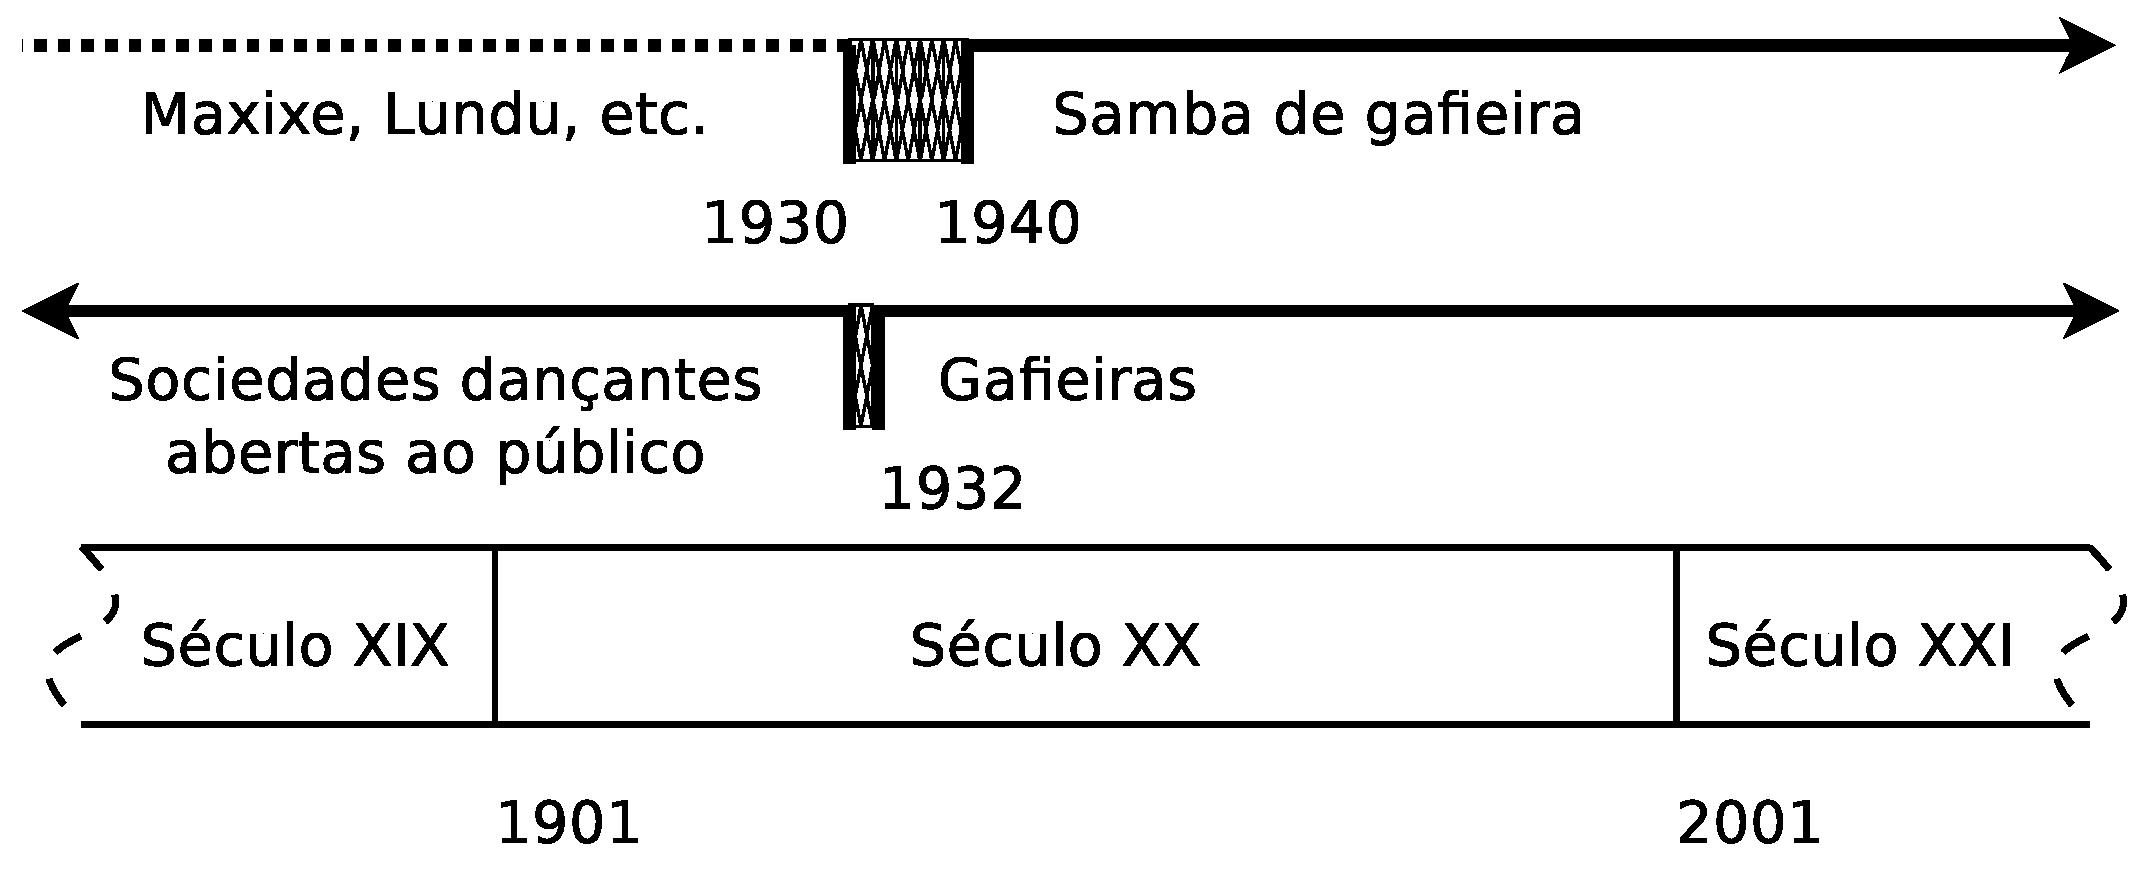
\includegraphics[width=1.0\textwidth]{chapters/cap-historia-sambagafieira/gafieira-crono.eps}
  \caption{ Cronologia da formação do samba de gafieira.}
\label{fig:sambagafieiracrono}
\end{figure}

%%%%%%%%%%%%%%%%%%%%%%%%%%%%%%%%%%%%%%%%%%%%%%%%%%%%%%%%%%%%%%%%%%%%%%%%%%%%%%%
%\clearpage
\section{Música para dançar samba de gafieira}
\label{subsec:gafieiradancaestilos}

Entre os estilos musicais em que o samba de gafieira (dança) se adapta bem, 
estão alguns dos subgêneros do samba; assim,
aqui mencionaremos uma lista de músicas que por sua graça, estilo e alegria,
a meu entender, podem ser dançados usando o samba de gafieira. Porem, 
estas músicas não pretendem ser máximos expoentes representativos, do subgênero em que estão agrupados;
e sim uma indicação ou orientação ao leitor, 
para treinar sua dança usando músicas em que possa ser mais confortável a experiencia.

\begin{itemize}
\item \textbf{Samba de gafieira (música)}
\begin{example} ~
\begin{itemize}
%\item ``Samba de padua'' interpretado pelo grupo Turma da Gafieira.
\item ``Samba de morro'' interpretado pelo grupo Turma da Gafieira.
%\item ``Piston da gafieira'' de Billy Blanco, interpretado por Jorge Beiga.
\item ``Piston da gafieira'' de Billy Blanco, interpretado por Zeca pagodinho \cite{barbosa2014zeca}.
\item ``Beija-me'' de Roberto Martins e Mário Rossi, interpretado por Zeca pagodinho \cite{barbosa2014zeca}.
\item ``Pisei num despacho'' de Geraldo Pereira e Elpídio Viana, interpretado por Zeca pagodinho \cite{barbosa2014zeca}.
%\item ``Tive sim'' de Cartola, interpretado por Zeca pagodinho \cite{barbosa2014zeca}.
%\item ``Tarzan, o filho do alfaiate'' de Noel Rosa e Vadico, interpretado por Zeca pagodinho \cite{barbosa2014zeca}.
%\item ``Se você visse'' de Dino 7 cordas e Del Loro, interpretado por Zeca pagodinho \cite{barbosa2014zeca}.
\end{itemize}
\end{example} 

\item \textbf{Samba de breque}
\begin{example} ~
\begin{itemize}
\item ``Baile no elite'' interpretado por Casuarina.
\item ``Eu sou a marrom'' interpretado por Alicione.
%\item ``Hoje sou diferente'' interpretado por Lenita Rodrigues.
\item ``Pra levantar poeira'' interpretado por Bodhar.
\end{itemize}
\end{example} 

\item \textbf{Pagode paulista (Sambalanço)}
\begin{example} ~
\begin{itemize}
\item ``Cheia de manias''  interpretado pelo grupo Raça Negra.
\end{itemize}
\end{example} 

\item \textbf{Partido alto}
\begin{example} ~
\begin{itemize}
%\item ``A língua'' interpretado por Beto lima.
\item ``Partido Alto'' interpretado por Aleh.
\end{itemize}
\end{example} 

\item \textbf{Pagode}
\begin{example} ~
\begin{itemize}
\item ``Trilha Do Amor''  interpretado pelo Grupo Revelação. 
\item ``A Batucada Te Pegou'' interpretado pelo Grupo Sou Muleke.
\item ``Dança da Solidão'' interpretado por Pagode de Mesa do álbum Terra Brasil. 
\item ``Eu e você sempre'' interpretado por Jorge Aragão
\end{itemize}
\end{example} 

\item \textbf{Samba-canção (música)}
\begin{example} ~
\begin{itemize}
\item ``Eu Quero E Sossego'' interpretado por Paulo Moura.
\item ``Só Louco'' interpretado por Luiz Melodia.
\item ``Você É a Fonte'' interpretado por  Quinteto em Branco e Preto.
\item ``Eu Quero é Sossego'' interpretado por Paulo Moura.
\end{itemize}
\end{example} 

\item \textbf{Bossa nova}
\begin{example} ~
\begin{itemize}
\item ``I Don't Know (Bossa Mix)'' interpretado por Erika do álbum ``I Don't Know''
\item ``Human Nature'' interpretado por Marcela Mangabeira.
\end{itemize}
\end{example} 


\item \textbf{Choro}
\begin{example} ~
\begin{itemize}
\item ``Choro de gafieira'' de Pixinguinha.
\item ``Chorinho de gafieira'' de Astor Silva.
\item ``Noites Cariocas'' de Jacob do Bandolim.
\end{itemize}
\end{example} 


\item \textbf{Samba-choro}
\begin{example} ~
\begin{itemize}
\item ``Escurinho'' interpretado por Corina Magalhães.
\item ``Tico Tico no Fubá'' interpretado por Leci Brandão.
\end{itemize}
\end{example}

\end{itemize}

A Figura \ref{fig:gafieiradancaestilos} mostra um resumo de alguns dos 
subgêneros do samba onde pode ser dançado o samba de gafieira.
\begin{figure}[h]
  \centering
    \includegraphics[width=0.7\textwidth]{chapters/cap-historia-sambagafieira/gafieiravcmusica.eps}
  \caption{ Subgêneros do samba onde pode-se dançar samba de gafieira.}
\label{fig:gafieiradancaestilos}
\end{figure}




\chapterimage{chapter_head_2.pdf} % Chapter heading image

\chapter{Regras na dança de salão}

Antes de iniciar as explicações no capítulo, 
é necessário partir desde uma linguagem comum;
com este propósito, 
significados de algumas palavras bem definidas na literatura são mostrados a continuação:
 
\begin{definition}[Regra:] 
\index{Regras}
\label{def:Regra}
Princípio que serve como padrão no estudo das artes e ciências \cite{priberamregra} \cite{dicioregra}.
Exemplo: regras gramaticais; regras de etiqueta; regras do jogo; regras na dança.
\end{definition}

\begin{definition}[Casal:] 
\index{Casal}
\label{def:Casal} O Dicionário Priberam da Língua Portuguesa \cite{priberamcasal} define casal como:
Par formado por um macho e uma fêmea.
Exemplo: casal de cavalos, casal de pombas, casal de humanos.
\end{definition}

\begin{definition}[Par:] 
\index{Par}
\label{def:Par} O Dicionário Priberam da Língua Portuguesa \cite{priberampar} define par como:
Igual, semelhante, parceiro.
Cada uma das pessoas que constituem uma dupla na dança.
\end{definition}


Usando como base os significados mostrados anteriormente, 
serão descritos alguns termos muito utilizados na dança\footnote{
Para as definições, foi priorizado o uso da palavra par sobre a palavra casal,
para poder definir às entidades dançantes independentemente do sexo dos participantes.}.
Assim,  são propostas as seguintes definições:

\begin{definition}[Paradigma da condução (Dança):] 
\index{Condução} 
\label{def:ParadigmaConducao} 
Este é um modelo de dança a dois usado na \hyperref[def:DancaSalao]{\textbf{dança de salão}},
\hyperref[def:DancaSocial]{\textbf{dança social}}, etc. 
E indica que entre as pessoas que conformam a dança, 
existe uma transmissão de informação relativa à movimentação e as pausas, no \hyperref[def:Par]{\textbf{par}} dançante; 
de modo que, a informação tem um fluxo unidirecional no médio de transmissão,
que vá desde o \hyperref[def:Condutor]{\textbf{condutor}} ate o \hyperref[def:Seguidor]{\textbf{seguidor}}. 
\end{definition}
\index{Condutor} 

\begin{definition}[Condutor (Dança):] 
\index{Condutor} 
\label{def:Condutor} 
A pessoa que tem o papel de conduzir ou propor o movimento ao \hyperref[def:Seguidor]{\textbf{seguidor}}. 
O objetivo técnico das pessoas que optam por este rol na dança, é chegar 
a ter a sensibilidade necessária para entender onde está localizado espacialmente, 
e como distribui o peso do corpo, o \hyperref[def:Seguidor]{\textbf{seguidor}}; 
de modo que seja possível para o condutor aplicar sobre o \hyperref[def:Seguidor]{\textbf{seguidor}}, 
uma mistura de indicações, forças e torções,  
para provocar os movimentos ou pausas desejadas;
chama-se a isto saber conduzir.
Sinônimos de condutor: Líder (Dança).
\end{definition}

\begin{definition}[Seguidor (Dança):] 
\index{Seguidor} 
\label{def:Seguidor} 
A pessoa que recebe a condução e proporciona uma resposta corporal. 
O objetivo técnico das pessoas que optam por este rol na dança, é chegar 
a ter a sensibilidade necessária para entender e incorporar as conduções,
independentemente de quem seja a pessoa que aplique a condução;
chama-se a isto ser conduzível.
Sinônimos de seguidor: Conduzido (Dança).
\end{definition}



\begin{definition}[Abraço de dança:]
\index{Abraço de dança}
\label{def:abracodedanca}  
É um abraço onde o \hyperref[def:Condutor]{\textbf{condutor}} 
rodeia com a mão direta as costas do \hyperref[def:Seguidor]{\textbf{seguidor}},
numa linha meia entre a linha dos ombros e a linha da parte baixa do tórax;
enquanto a mão esquerda, do condutor, segura com o braço semi flexionado a mão direita do seguidor,
colocando ambas mãos a altura do ombro da pessoa mais baixa do \hyperref[def:Par]{\textbf{par}}.
\end{definition}


\begin{definition}[Firmeza de braços (Dança):]
\index{Firmeza de braços}
\label{def:brazosfirmes} 
Que o \hyperref[def:Condutor]{\textbf{condutor}} e \hyperref[def:Seguidor]{\textbf{seguidor}}
tenham os braços firmes, não implica fazer força pra submeter ao par;
e sim, ativar os músculos o mínimo e necessário para manter a posição relativa e postura dos braços.
de modo que a informação de condução passe a traves dos braços e chegue, com fidelidade, ao corpo do seguidor.

Outra forma de descrever a firmeza dos braços, 
é indicando que esta ação implica ter uma ativação muscular e auto controle, 
para suprimir conscientemente alguns graus de liberdade que existem nos braços, 
dependendo da situação e do estilo de dança.
Alguns destes graus de liberdade são obtidos devido a:
\begin{itemize}
\item O movimento de flexão no pulso,
\item movimento de rotação no antebraço,
\item movimento de flexão no cotovelo,
\item movimentos de rotação e abertura no ombro.
\end{itemize}
\end{definition}



Para finalizar as definições neste capítulo, foram tomados dois conceitos do artigo,
``Conceitos e definição de Dança de Salão'' \cite{Zamoner2012};
e modificações foram feitas para adaptar as definições aos conceitos de \hyperref[def:Condutor]{\textbf{condutor}} e \hyperref[def:Seguidor]{\textbf{seguidor}}, usados ao longo deste livro.

\begin{definition}[Dança social:]
\index{Dança social} 
\label{def:DancaSocial} 
É uma dança com fim recreativo de prática social, não cênica, nem competitiva, 
que não tem um interesse artístico, histórico, geográfico ou técnico; 
que se universaliza e consiste na movimentação dos corpos do \hyperref[def:Par]{\textbf{par}} de dança  \cite{Zamoner2012}, 
onde existe o rol do \hyperref[def:Condutor]{\textbf{condutor}} 
e do \hyperref[def:Seguidor]{\textbf{seguidor}} (papeis intercambiáveis), 
ate onde o nível técnico do par o permita.
\end{definition}

\begin{definition}[Dança de salão:]
\index{Dança de salão}
\label{def:DancaSalao}  
É uma arte que procura conservar suas características técnicas, 
sua origem histórica e geográfica, e se universaliza em práticas sociais. 
Esta arte consiste na interpretação improvisada da música por médio dos movimentos 
dos corpos de um \hyperref[def:Par]{\textbf{par}} de dança \cite{Zamoner2012}, 
utilizando o \hyperref[def:ParadigmaConducao]{\textbf{paradigma da condução}} .
\end{definition}

\PRLsep{*}

Neste capítulo veremos um conjunto de \hyperref[def:Regra]{\textbf{regras}}, 
e a explicação de como o cumprimento ou não destas, 
afetam ao desenvolvimento estético e técnico da \hyperref[def:DancaSalao]{\textbf{dança de 
salão}}\footnote{Ou na \hyperref[def:DancaSocial]{\textbf{dança social}} sim se está interessado em levar estas ideias a esse âmbito.}  no \hyperref[def:ParadigmaConducao]{\textbf{paradigma da condução}}.

As \hyperref[def:Regra]{\textbf{regras}} que veremos neste capítulo não devem ser
tratadas como leis, e sim como diretrizes a serem usadas como padrão de inicialização, de modo que 
os dançarinos analisarão cada caso e se necessário criarão uma exceção e atuará conforme ela.

Serão usados neste capítulo termos como \hyperref[def:Condutor]{\textbf{condutor}} e \hyperref[def:Seguidor]{\textbf{seguidor}}; 
mas, não existe nenhuma obrigatoriedade ou restrição para as pessoas, 
na escolha de algum destes papéis na dança.
Porem, é comum ver que o papel de condutor é escolhido tradicionalmente pelos homens e o papel de seguidor pelas mulheres.
%só são um recurso literário para o melhor entendimento das explicações mostradas aqui.
\begin{lattention}
É importante aclarar
que as regras expostas neste capítulo não estão regulamentadas por nenhuma entidade ou instituição; assim, estas
refletem, o meu aprendizado de distintos professores,
interpretações pessoais  e deduções. 
\end{lattention}

%%%%%%%%%%%%%%%%%%%%%%%%%%%%%%%%%%%%%%%%%%%%%%%%%%%%%%%%%%%%%%%%%%%%%%%%%%%%%%%%
\section{Regras gerais na dança de salão}
\label{sec:regrasgeral}
\index{Regras!Dança de salão}

A continuação são listadas algumas regras gerais na dança de salão, 
que abrangem um conjunto amplo de estilos de dança.\\

\begin{description}

\item[Rodar o salão:] Que os dançarinos executem sua dança girando o salão, 
é importante para criar a ilusão de que o espaço de dança é maior, dado que mesmo
tendo uma pista de dança lotada, ao rodar o salão, o espaço que um
\hyperref[def:Par]{\textbf{par}} deixa ao se movimentar é ocupado pelo \hyperref[def:Par]{\textbf{par}} que vem atrás deles, criando 
assim um fluxo de movimento circular que permite a todos os casais usar a pista de dança
na sua totalidade (por convenção o sentido de giro é sempre anti-horário); 
visto o anterior é importante ressaltar que né todas as danças tem
uma evolução circular na pista de dança, pois existem estilos de dança que são dançados em linha,
como por exemplo a ``Salsa em linha'' ou o ``West coast swing''; ou também existem estilos que
tem um comportamento hibrido entre circular e linha como o "Zouk". Neste sentido,
a ``samba de gafieira'' tem um comportamento circular e  deve ser dançado
rodando o salão para um boa etiqueta na pista de dança.


\item[Conduzir e ser conduzidos:] Trabalhar num \hyperref[def:ParadigmaConducao]{\textbf{paradigma da dança baseado
na condução}} é muito importante para na \hyperref[def:DancaSalao]{\textbf{dança de salão}}, dado que isto implicará
que um \hyperref[def:Condutor]{\textbf{condutor}} habilidoso, poderá dançar fluidamente com pessoas com quem nunca dançou
antes (se esta for conduzível). De forma similar acontecerá para os \hyperref[def:Seguidor]{\textbf{seguidores}} que desenvolvam
a sensibilidade necessária para serem conduzíveis, elas poderão dançar com qualquer
condutor, inclusive poderão ter um desenvolvimento básico em estilos de dança pouco ou não conhecidos.

O caso oposto ao \hyperref[def:ParadigmaConducao]{\textbf{paradigma da condução}}, é ter um estilo de dança baseado em coreografias;
este enfoque, dependendo da finalidade, pode ser visto como um vicio que geralmente aparece quando iniciamos
na dança. 
\begin{example}
Quando a pessoa que deve conduzir, assume que se esta realiza a parte do movimento 
que lhe corresponde, sem enviar nenhuma informação ao \hyperref[def:Par]{\textbf{par}}, 
então o \hyperref[def:Seguidor]{\textbf{seguidor}} deve reconhecer/adivinhar e realizar o movimento que o condutor imaginou.
\end{example} 
O enfoque do exemplo anterior, funciona bem quando ambos dançarinos tem treinado antecipadamente os movimentos, 
e/ou conhecem a sequencia em que estes movimentos serão executados; 
porem, falha quando os dançarinos não se conhecem.
Comprovar isto é fácil se imaginamos, por exemplo, o caso em que o \hyperref[def:Condutor]{\textbf{condutor}} executa um movimento
que tem a parte inicial muito parecida a outro movimento, nesse caso, se o \hyperref[def:Seguidor]{\textbf{seguidor}} não tiver
um poder telepático confundirá um movimento com o outro e acontecerá um problema de comunicação. Assim, a coreografia
na dança deve estar reservada para apresentações, onde o \hyperref[def:Par]{\textbf{par}} volta 
a sua atenção para a encenação da peça, e não para detalhes mais mecânicos.

\item[Peso do corpo definido num pé:] Em estilos de dança onde uma boa postura é requerida,
ter o peso total do corpo bem definido sobre um pé, 
ao final de cada ação ou proposta de movimento,
quando sabemos que realizaremos mais movimentos imediatamente depois;
garante conservar a postura e ter uma maior velocidade no tempo de reação para o seguinte movimento;
pois, ao ter um pé livre poderemos mover ele sem temor a perder o equilibro, 
o que se traduz na leveza na execução dos movimentos. 
Isto é facilmente comprovável se fazemos um pequeno exercício. 
\begin{example}
Ao ficar em pé separamos as
pernas uma distancia igual à de nosso quadril, e nesse momento levamos o peso do corpo\footnote{
Em física podemos representar um corpo como um objeto com a masa concentrada no seu centro de gravidade, 
que no casso do ser humano está perto do umbigo.} a
apontar a um ponto médio entre nossos pés, nesse instante estamos dividindo o peso do corpo
entre nossos dois pontos de apoio, 50$\%$ no pé direito e 50$\%$ no pé esquerdo; agora, mantendo o peso
do corpo nesse lugar, tentaremos levantar qualquer de nossos pés, será evidente
que esse trabalho é muito difícil sem perder o equilíbrio, pois para mantê-lo
precisamos de ambos pontos de apoio; casos similares podem ser vistos com qualquer proporção de distribuição de peso,
por exemplo, 30$\%$ e 70$\%$ ou 20$\%$ e 80$\%$. 
\end{example}
Assim, do exemplo anterior se deduz, que estaremos
equilibrados, e poderemos executar nossos movimentos e levantar um pé 
mantendo a postura e auto controle, quando
temos o 100$\%$ do peso do corpo num pé só, o pé de apoio.
 
Por outro lado, quando consideramos ao 
\hyperref[def:Condutor]{\textbf{condutor}} como o agente desequilibrante do \hyperref[def:Seguidor]{\textbf{seguidor}}, 
por exemplo no caso em que este aplica uma condução;
a regra de manter o peso do corpo num pé só, tem um valor agregado; 
pois fica mais fácil para o condutor orientar
ao seguidor a fazer o seguinte movimento, dado que o único pé que o seguidor pode mover é o pé
que está livre, e que é o pé que o condutor precisa que se movimente, 
além de que a força necessária pelo condutor para tirar ao seguidor do seu equilíbrio 
atual é muito menor ao caso quando o seguidor tem dois pontos de apoio.
Adicionalmente o seguidor tem um pé livre para se resguardar do desequilíbrio, provocado pelo 
condutor, e adquirir um novo equilíbrio com esse pé.

\textbf{Nunca podemos dividir o peso do corpo?} Esta caraterística é possível sim,
se nossa dança fosse um relato escrito, o peso de nosso corpo deve estar bem definido num pé,
ao final de cada palavra, em cada virgula e ponto e virgula; por outra lado, 
o peso do corpo pode estar dividido em cada ponto.

\textbf{Este é o único meio de manter o equilíbrio na dança?}  Não, 
existem estilos de dança, como por exemplo no ``lindy hop'' onde se consegue manter os pês libres, 
para executar os movimentos, mantendo um equilíbrio dinâmico,
realizando um movimento de rebote (chamado ``bouncing'') ao ritmo da música.
O movimento consiste em deixar cair nosso corpo, flexionando ligeiramente  os joelhos, 
e imediatamente volver a ficar em pé, realizando assim um efeito de mola. 

\item[Ter uma boa conexão entre o par na dança:] Seguindo a ideia da condução, esta só pode
ser realizada se existe um médio de comunicação, onde possa ser transmitido
o comando do \hyperref[def:Condutor]{\textbf{condutor}} ao \hyperref[def:Seguidor]{\textbf{seguidor}}. 
Assim, um boa conexão garante este fluxo de informação entre o \hyperref[def:Par]{\textbf{par}} na dança. 
A forma exata de obter esta conexão varia ligeiramente entre os diferentes estilos de dança;
dado que em alguns casos será usado um \hyperref[def:abracodedanca]{\textbf{abraço de dança}} 
e em outros o par estará conectado segurando-se das mãos.
Mas, em todos os casos, 
o que se procurará é ter a maior quantidade de pontos de contato no par,
pois quanto mais pontos de contato tenhamos, 
maior será a fidelidade com que a informação da condução chegue ao seguidor.


Outro ponto importante desta conexão é a \hyperref[def:brazosfirmes]{\textbf{firmeza dos braços}}, 
pois é a traves deles que passa a maior parte da informação.
Assim, no caso do seguidor, ter os braços firmes implicará que qualquer informação que chegue por eles,
se transmitirá maioritariamente ao corpo,
mudando assim este de estado ou posição.

Em estilos de dança onde existe a possibilidade de dançar tomados das mãos,
se não se tem bem treinados os braços,
é muito fácil que a informação da condução seja perdida.
Isto acontece, porque no braço todo, temos vários graus de liberdade nas articulações.
Se algum destes pontos não tem a firmeza necessária para transportar a informação de condução, 
sem modificar maioritariamente sua posição relativa e postura,  
então esse ponto provocará a perdida da informação, 
pois se modificará a posição dos braços sem alterar a posição do corpo.
\begin{example}
De pie frente a frente com seu par, testaremos 3 tipos de condução, 
criadas quando o condutor segura com as mãos ao seguidor, em 3 lugares diferentes:
\begin{itemize}
\item Segurando num ponto meio entre entre o cotovelo e os ombros,
\item segurando no antebraço, e
\item tomados das mãos.
\end{itemize}
\end{example}
No exemplo anterior, será muito evidente em seguidores iniciantes,
que a maior eficacia na transmissão de informação se consegue segurando entre os cotovelos e os ombros,
seguido por segurar pelo antebraço, e finalmente nas mãos;
é dizer, a eficacia na transmissão da informação, 
diminuí com o aumento dos grãos de liberdade.

Assim, para obter uma boa conexão no par, 
e eficacia na transmissão de informação, devemos ter:
\begin{itemize}
\item Uma boa postura de braços e
\item procurar a maior quantidade de pontos de contato.
\end{itemize}  

\end{description}

%%%%%%%%%%%%%%%%%%%%%%%%%%%%%%%%%%%%%%%%%%%%%%%%%%%%%%%%%%%%%%%%%%%%%%%%%%%%%%%%
\section{Regras gerais na samba de gafieira}
\label{sec:regrassambagafieira}
\index{Regras!Samba de gafieira}

É evidente olhando aos profissionais da dança,
que cada pessoa tem uma forma particular de dançar, 
que carateriza e identifica a ela. Porem, 
dentro desse margem pessoal de trabalho, 
pode ser identificado que a pessoa está realizado um estilo de dança em particular,
por exemplo: samba de gafieira, forró, salsa, etc.
Assim, se conclui que existe um conjunto de caraterísticas na dança,
que provocam que estas sejam enquadradas num estilo particular;
estas caraterísticas não são todo ou nada, é dizer, 
não precisam cumprir-se todas para reconhecer um estilo de dança,
porem, quanto maior sejam as caraterísticas usadas mais fácil será enquadrar uma dança num estilo de dança em particular.

As regras planteadas aqui, são uma tentativa de enumerar as caraterísticas,
que tenho observado, que provocam que um espectador ou dançarino,
vejam ou percebam que se está dançando samba de gafieira.
\begin{description}
\item[Quadril avança, ombros e pé acompanham:]  Os movimentos, na samba de gafieira, iniciam no quadril;
isto provocará que as demais partes do corpo (pernas e torço) atuem a consequência para achar um novo equilíbrio.
Adicionalmente ajudará a que ao terminar o movimento, o peso de nosso corpo esteja bem posicionado sobre um pé só.
\item[Chegar com 100$\%$ do peso do corpo, quando se movimenta um pé :] 
Uma característica da sam- ba de gafieira é uma estética que evoca à malandragem, 
uma forma de obter esta estética é que ao movimentar um pé, este ao tocar o chão,
debe chegar com o 100\% do peso do corpo; realizar esta ação é fácil, 
se temos cumprido que nosso movimento inicie desde o quadril e não por esticar as pernas.

Assim, existe uma diferença com outros estilos de dança, 
como o bolero e o tango, 
onde se procura projetar uma estética de elegância;
nestes estilos, no movimento dos pés, primeiro se aponta com a ponta do pé sem levar o peso do corpo,
 e logo o peso é transferido ao lugar apontado, numa dinâmica continua de aponta e transfere.

Isto não quer dizer que a dinâmica de aponta e transfere não possa ser usada em gafieira,
e sim que o dançarino deve escolher que imagem deseja projetar em cada momento,
malandragem, elegância ou misturas. 

\item[Ter um bom abraço na samba de gafieira:] Como já foi mencionado na Seção \ref{sec:regrasgeral}, 
ter uma boa conexão na dança é muito importante para uma boa transferência de informação na condução; 
porem, existem particularidades desta conexão na samba de gafieira que devem ser ressaltadas.

Por exemplo, na maioria de movimentos se usa o \hyperref[def:abracodedanca]{\textbf{abraço de dança}};
mas, particularmente em samba de gafieira, se precisa que o braço esquerdo da dama tenha contato
e rodeie, pela parte externa, ao braço direito do condutor; 
de modo  que o seguidor não se debruce sobre o condutor,
e sim que mantenha um atrito entre os braços.
A importância deste contato radica em que o condutor em algumas situações precisam transmitir conduções, 
que provoquem a sacada de perna do seguidor (ex: Edmundo, sacadas, etc.), 
e isto e transmitido realizando o condutor um movimento de rotação do tórax no plano axial.  
Rotando em sentido horário para tirar a perna direita do seguidor, 
e em sentido anti-horário para tirar a perna esquerda do seguidor;
é neste ponto que esse atrito entre os braços é importante, 
pois quando se realiza o movimento de rotação anti-horário, se não existisse o atrito,
o tórax do condutor giraria só, sem afetar o tórax do seguidor ou afetando muito pouco;
assim, o atrito garante que esta informação na torção chegue com maior eficacia ao seguidor.

Por outro lado, em alguns momentos na dança, de samba de gafieira, usaremos um abraço de dança mais separado,
para realizar passos como o ``picadilho''; em estas circunstancias, é o braço direito do seguidor,
que precisa em todo momento estar \hyperref[def:brazosfirmes]{\textbf{firme}}, 
mantendo uma ativação muscular e diminuição dos graus de liberdade,
para que toda a informação enviada pelo condutor atravesse os braços e o tórax do seguidor,
e chegue sem degradação ate o quadril, onde se provocará a movimentação de pés planejada pelo condutor.

\item[Abraço uniforme do condutor:] Continuando com as particularidades do abraço,
mas agora no âmbito da distancia de separação entre o \hyperref[def:Par]{\textbf{par}} durante o tempo que dure o abraço.
É importante ressaltar que deves-se manter uma regularidade na distancia de separação,
e evitar um ``abraço sanfona'', é dizer um abraço onde o condutor as vesses, 
aperta demais ao seguidor, e outras vesses onde deixe ele solto e mais separado dele.
É claro que esta irregularidade do abraço, existe na dança; 
mas, esta deve ser uma coisa consciente e projetada 
pelo condutor em função da técnica necessária para realizar um passo; 
e em nenhum caso deve ser uma coisa  fora de controle ``sanfonando'' ao par.

Um momento onde é altamente importante esta regularidade, 
é durante passos como ``gancho redondo''.
Por outro lado, termos momentos em que precisaremos ajustar a distancia do abraço,
antes do inicio do passo, para mais perto no caso do ``pião'' e para mais longe no caso do ``picadilho''.

\item[Procurar o paralelismo de ombros no par:] 
Um ponto muito cobrado, na dança de salão é manter a linha de visão no \hyperref[def:Par]{\textbf{par}},
em samba de gafieira esta caraterística é obtida mantendo sempre paralelas, as linhas dos ombros, no par.
Isto além de um ganho estético, tem interessantes caraterísticas técnicas;
pois se a combinamos com a ideia de manter sempre a mesma distancia no par;
chegamos a um ponto onde poderemos estabelecer uma condução por indução, ou condução sem contato.

A responsabilidade de manter este paralelismo de ombros é do \hyperref[def:Seguidor]{\textbf{seguidor}},
pois este deve ``seguir'' o movimento do \hyperref[def:Condutor]{\textbf{condutor}}.
Por outro lado o condutor tem a responsabilidade de realizar os movimentos com uma velocidade e clareza necessárias, 
para que estes possam ser acompanhados pelo seguidor.

\item[Conduzir pelo tórax não pelos braços:] 
Se conseguimos ter paralelismo na linha dos ombros,
e se procuramos manter sempre a mesma distancia, 
e linha de visão com o \hyperref[def:Par]{\textbf{par}}, 
sem a necessidade do uso dos braços;
pode-se deduzir que, nestas dinâmicas corporais,
é o tórax do \hyperref[def:Condutor]{\textbf{condutor}} quem guia ao \hyperref[def:Seguidor]{\textbf{seguidor}}.
Isto implica que os braços tem o papel de brindar sustento para a transferência de informação da condução,
porem os braços do condutor, não são os executantes e protagonistas da condução;
sendo, principalmente o tórax do condutor, a fonte mecânica desta informação.
Este dado é muito relevante em passos como o ``Romário'' ou o ``gancho redondo'',
onde é o tórax, e não os braços, do condutor que leva ao seguidor de um lado a outro. 

\item[O pé de apoio deve apontar ao par:] 
Quando nos encontremos numa postura, em que o peso do corpo está definido totalmente num pé;  
é dizer, quando não estejamos num movimento de transferência de peso;
o pé que contem o peso do corpo debe apontar a um ponto médio entre os pés do \hyperref[def:Par]{\textbf{par}} de dança.
Esta caraterística tem um proposito além de estético, técnico;
dado que o corpo tende a ir em direção a onde esta apontando nosso pé,
assim ao apontar sempre ao par, 
garantimos que em todo momento procuraremos a proximidade e teremos uma linha de visão  com ele.
Uma boa metáfora, é pesar que a ponta de nosso pé é uma bússola que aponte ao norte que é nosso par.
\end{description}


%%%%%%%%%%%%%%%%%%%%%%%%%%%%%%%%%%%%%%%%%%%%%%%%%%%%%%%%%%%%%%%%%%%%%%%%%%%%%%%%
%% CAPITULO
%%%%%%%%%%%%%%%%%%%%%%%%%%%%%%%%%%%%%%%%%%%%%%%%%%%%%%%%%%%%%%%%%%%%%%%%%%%%%%%%
\chapterimage{chapter_head_2.pdf} % Chapter heading image

%%%%%%%%%%%%%%%%%%%%%%%%%%%%%%%%%%%%%%%%%%%%%%%%%%%%%%%%%%%%%%%%%%%%%%%%%%%%%%%
%%%%%%%%%%%%%%%%%%%%%%%%%%%%%%%%%%%%%%%%%%%%%%%%%%%%%%%%%%%%%%%%%%%%%%%%%%%%%%%
%%%%%%%%%%%%%%%%%%%%%%%%%%%%%%%%%%%%%%%%%%%%%%%%%%%%%%%%%%%%%%%%%%%%%%%%%%%%%%%
%%%%%%%%%%%%%%%%%%%%%%%%%%%%%%%%%%%%%%%%%%%%%%%%%%%%%%%%%%%%%%%%%%%%%%%%%%%%%%%
\chapter{Passos do samba de gafieira}
\label{chap:passos-samba-gafieira}
%\index{Passos}


\begin{definition}[Plano axial:] 
\index{Plano axial}
\label{def:PlanoAxial}
O Dicionário Priberam da Língua Portuguesa \cite{priberamplano} define plano axial como:
Plano transversal, plano horizontal que divide o corpo ou uma estrutura anatômica em parte superior e parte inferior.
Ver Figura \ref{fig:bodyhumanplane}.
\end{definition}

\begin{definition}[Plano frontal:] 
\index{Plano frontal}
\label{def:PlanoFrontal}
O Dicionário Priberam da Língua Portuguesa \cite{priberamplano} define plano frontal como:
Plano coronal,   plano vertical e paralelo à sutura coronal do crânio, que divide o corpo em parte anterior e parte posterior.
Ver Figura \ref{fig:bodyhumanplane}.
\end{definition}

\begin{definition}[Plano sagital:] 
\index{Plano sagital}
\label{def:PlanoSagital}
O Dicionário Priberam da Língua Portuguesa \cite{priberamplano} define plano sagital como:
Plano vertical e paralelo à sutura sagital do crânio, que divide o corpo em parte direita e parte esquerda.
Ver Figura \ref{fig:bodyhumanplane}.
\end{definition}

\begin{figure}[h!]
  \centering
    \includegraphics[width=0.60\textwidth]{body-plane/files/body-plane.png}
  \caption{ Planos e eixos no corpo humano.}
\label{fig:bodyhumanplane}
\end{figure}

\begin{definition}[Eixo axial:] 
\index{Eixo axial}
\label{def:EixoAxial}
É o eixo perpendicular ao plano axial.
Ver Figura \ref{fig:bodyhumanplane}.
\end{definition}

\begin{definition}[Eixo frontal:] 
\index{Eixo frontal}
\label{def:EixoFrontal}
É o eixo perpendicular ao plano frontal.
Ver Figura \ref{fig:bodyhumanplane}.
\end{definition}

\begin{definition}[Eixo sagital:] 
\index{Eixo sagital}
\label{def:EixoSagital}
É o eixo perpendicular ao plano sagital.
Ver Figura \ref{fig:bodyhumanplane}.
\end{definition}

\begin{definition}[Passo cíclico:] 
\index{Passo cíclico}
\label{def:PassoCiclico}
É um passo de dança que pode acontecer por um tempo indeterminado,
devido a que este está composto por ciclos, cuja postura de inicio e final é a mesma.
\end{definition}

\begin{definition}[Passo simétrico:] 
\index{Passo simétrico}
\label{def:PassoSimetrico}
É um passo de dança que tem a primeira metade do passo similar à segunda,
com a diferencia que se executa com os pés intercambiado (direita por esquerda)
ou com as posições dos corpos intercambiadas (seguidor por condutor).
\end{definition}

\begin{definition}[Duração do movimento:] 
\index{Duração do movimento}
\label{def:DuracaoDoPasso}
Ou a \textbf{duração do passo}, 
é a longitude temporal de um passo de dança, contado em tempos da música.
No caso de \hyperref[def:PassoCiclico]{\textbf{passos cíclicos}}, a duração do passo se refere a duração do ciclo.
\end{definition}


\begin{definition}[Dançar no tempo forte:] 
\index{Dançar no tempo forte}
\label{def:DancaNoTempo}
Ou simplesmente \textbf{dançar no tempo}, indica que se está dançando com passos com o movimento principal ou inicial (dependendo do estilo de dança), 
se executando no tempo forte da música; ver Exemplo \ref{example:dancatempoforte}.
\end{definition}
\begin{example}
\label{example:dancatempoforte}
Se definimos um passo de dança como: Pisar, usando um pé cada vez, 
realizando um movimento com uma distribuição espacial, junto-junto-longo;
e definimos ao movimento ``longo'' como o movimento principal. 
Se executássemos o movimento ``longo'' no tempo forte, o passo junto-junto-longo,
estaria sendo dançado no tempo forte.
\end{example}

\begin{definition}[Dançar em contratempo:] 
\index{Dançar no contratempo}
\label{def:DancaNoContratempo}
Indica que se está dançando, com o movimento principal ou inicial (dependendo do estilo de dança) do passo, 
executando-se em contra do tempo forte da música; é dizer, executando-se num tempo fraco (em contratempo).
Com diferencia de \hyperref[def:DancaNoTempo]{\textbf{dançar no tempo forte}}, 
que é único, pois só existe um tempo forte;
existem varias formas de dançar como o movimento principal em algum tempo fraco; ver Exemplo \ref{example:dancatempofraco}.
\end{definition}
\begin{example}
\label{example:dancatempofraco}
Se definimos um passo de dança como: Pisar, usando um pé cada vez, 
realizando um movimento com uma distribuição espacial, junto-junto-longo;
e definimos ao primeiro movimento ``junto'' como o movimento principal. 
Se executássemos o movimento ``longo'' no tempo forte, o passo junto-junto-longo,
estaria sendo dançado em contratempo.
\end{example}

\begin{definition}[Passo a contratempo:] 
\index{Passo a contratempo}
\label{def:PassoAContratempo}
É um passo de dança cuja execução promove que quando se esteja dançando com um pé especifico acompanhando o tempo forte da música,
ao finalizar o passo este pé esteja sendo marcado no tempo fraco.
É dizer, são movimento onde após de realizados, 
passamos de \hyperref[def:DancaNoTempo]{\textbf{dançar no tempo}} a 
\hyperref[def:DancaNoContratempo]{\textbf{dançar no contratempo}} e vice-versa. 
No samba de gafieira, isto acontece quando o número de tempos musicais que o passo  usa é impar;
pois as músicas tradicionalmente são escritas sombre compassos binários, 
pelo que comumente acharemos um tempo forte intercalado por uno tempo fraco.
\end{definition}

\begin{definition}[Passo de deslocamento:] 
\index{Passo de deslocamento}
\label{def:PassoDeDeslocamento}
É um passo de dança cujo propósito, consequência ou objetivo é o deslocamento no salão.
\end{definition}

\begin{definition}[Postura de finalização:] 
\index{Postura, tipos!Postura de finalização}
\label{def:PosturaFinaliza}
É uma postura a qual da a percepção, 
de que se tem chegado ao ponto final da ideia expressada com o movimento.
Se nossa dança fosse um relato escrito, esta postura seria equivalente a um ponto ou ponto e virgula.
\end{definition}

\begin{definition}[Postura de transição:] 
\index{Postura, tipos!Postura de transição}
\label{def:PosturaTransicao}
É uma postura a qual da a percepção, 
de que não se tem completado a ideia expressada com o movimento, e que possivelmente vem mais algum outro movimento.
Se nossa dança fosse um relato escrito, esta postura seria equivalente a uma virgula ou espaço em branco entre as palavras.
\end{definition}



%%%%%%%%%%%%%%%%%%%%%%%%%%%%%%%%%%%%%%%%%%%%%%%%%%%%%%%%%%%%%%%%%%%%%%%%%%%%%%%
%%%%%%%%%%%%%%%%%%%%%%%%%%%%%%%%%%%%%%%%%%%%%%%%%%%%%%%%%%%%%%%%%%%%%%%%%%%%%%%
%%%%%%%%%%%%%%%%%%%%%%%%%%%%%%%%%%%%%%%%%%%%%%%%%%%%%%%%%%%%%%%%%%%%%%%%%%%%%%%
\section{\textcolor{blue}{Que passos existem no samba de gafieira?}}

No ano \AnoLivro~ podemos ver uma grande variedade de passos para o samba de gafieira,
tantos como a imaginação possa atingir, pois além dos movimentos mais conhecidos e  consagrados da dança,
podem existir variações  destes ou simplesmente estilos em que estos são realizados. 



Nas seguintes subseções, listaremos e descreveremos 
alguns dos passos que são possíveis de ver no samba de gafieira;
mas, estas descrições não pretendem ser uma guia de ensino,
e sim um instrumento para saciar a curiosidade do leitor em como os movimentos são realizados.\\

%%%%%%%%%%%%%%%%%%%%%%%%%%%%%%%%%%%%%%%%%%%%%%%%%%%%%%%%%%%%%%%%%%%%%%%%%%%%%%%
%%%%%%%%%%%%%%%%%%%%%%%%%%%%%%%%%%%%%%%%%%%%%%%%%%%%%%%%%%%%%%%%%%%%%%%%%%%%%%%
\PRLsep{Passos no samba de gafieira ate 1949}
%%%%%%%%%%%%%%%%%%%%%%%%%%%%%%%%%%%%%%%%%%%%%%%%%%%%%%%%%%%%%%%%%%%%%%%%%%%%%%%
\subsection{Balão} 
\label{def:PassoBalao}
\index{Passo!Balão}
\index{Passo a contratempo!Balão}
%%                CICLICO    |SIMETRICO   |CONTRATEMPO   |DESLOCAMENTOS |TIEMPOS
\caracterpasso{\NoCheckedItem}{\NoCheckedItem}{\CheckedItem}{\NoCheckedItem}{3}
Um movimento com este nome já existia desde as origens do samba nas gafieiras, 
sendo este movimento proveniente do maxixe \cite[pp. 142]{perna2002samba} 
\cite[pp. 93]{efege1974maxixe} \cite[pp. 465]{marcondes1977enciclopedia}.
%porem não tem se achado referencias sobre as caraterísticas do movimento no maxixe.



Seguindo o Prof. Gino Fornaciari, no ano 1947,  em São Paulo, se usava o nome balão e pião,
para representar a um mesmo movimento, um que agora chamaríamos de pião, 
porem o pião de 1947 era em sentido anti-horário \cite[pp. 68-72]{fornaciari1947aprender}.
Por outro lado, no seu livro ``Como apender a dançar'' (1950) 4ta edição,
o Prof. Fornaciari descreve um movimento  chamado ``Calçada'', com uma descrição semelhante 
ao ``balão'' de \AnoLivro~ \cite[pp. 162]{fornaciari1950aprender}.

Em \AnoLivro, o nome balão designa a um movimento que pode ser considerado aéreo, 
pois o \hyperref[def:Condutor]{\textbf{condutor}} tira do chão os pés do \hyperref[def:Seguidor]{\textbf{seguidor}}.
Um movimento com estas caraterísticas pode ser visto no filme ``Aviso aos navegantes'' (1950),
pelo que podemos especular que este era de uso comum desde muito antes \cite[min. 40:35]{AtlantidaDance};
porem, não pode-se souber sim lhe era atribuído ou não nessa época o nome de balão; 
mas pela semelhança com o movimento de quadril do passo chamado balão apagado,
é provável que sim, 
pois lembremos que o problema da homologação da nomenclatura dos passos existe ate em  nossos dias.



O movimento dura 3 tempos, o passo inicia com o seguidor ao lado direito do condutor, 
ligeiramente atrás dele, com um \hyperref[def:abracodedanca]{\textbf{abraço de dança}} 
bem próximo e uma postura similar à \hyperref[def:X-position]{\textbf{posição de X}} só que com os pés mais juntos.
No primeiro tempo o condutor da um passo ao lado, e pisa com o pé direito,
de modo que o seguidor fique em pé atrás da perna direita do condutor, sem perder o abraço.
No segundo tempo, aproveitando a postura, 
o condutor faz um movimento circular anti-horário com seu quadril, no \hyperref[def:PlanoAxial]{\textbf{plano axial}},
de modo que sua perna direita, que está em contato com a perna direita do seguidor,
serva como alavanca para tirar ao seguidor do chão, 
e este gire ou voe ao redor \footnote{O giro do seguidor é com o corpo reto e pernas juntas, 
como se fosse uma fita solta de um lado e com o outro lado presso num ponto 
que provoca o giro da fita no \hyperref[def:PlanoAxial]{\textbf{plano axial}}, com giro ao redor do eixo axial.} 
do condutor em sentido anti-horário.
No terceiro tempo o seguidor senta-se, é dizer faz uma cadeirinha, sobre a perna esquerda do condutor,
que para receber ao seguidor  da um passo ao frente.

\begin{comment}
A Figura \ref{fig:balao1950} mostra um fotograma do filme ``Aviso aos navegantes'' (1950),
onde se observa o inicio do passo balão (\AnoLivro), quando a moça tira os pés do chão.
\begin{figure}[h!]
  \centering
    \includegraphics[width=0.7\textwidth]{chapters/cap-historia-passos/balao1950.png}
  \caption{Fotograma com o inicio do passo balão (\AnoLivro), do filme ``Aviso aos navegantes'' (1950) \cite[min. 40:35]{AtlantidaDance}.}
  \label{fig:balao1950}
\end{figure} 
\end{comment}

%%%%%%%%%%%%%%%%%%%%%%%%%%%%%%%%%%%%%%%%%%%%%%%%%%%%%%%%%%%%%%%%%%%%%%%%%%%%%%%
\subsection{Balão apagado}
\index{Passo!Balão apagado} 
\index{Passo cíclico!Balão apagado}
\index{Passo simétrico!Balão apagado}
%%                CICLICO     |SIMETRICO   |CONTRATEMPO   |DESLOCAMENTOS |TIEMPOS
\caracterpasso{\CheckedItem}{\CheckedItem}{\NoCheckedItem}{\NoCheckedItem}{4}
Um movimento com este nome já existia desde as origens do samba nas gafieiras, 
sendo este movimento proveniente do maxixe \cite[pp. 142]{perna2002samba} \cite[pp. 68]{efege1974maxixe}.
Um exemplo do movimento que agora designamos como balão apagado pode 
ser visto no filme ``Aviso aos navegantes'' (1950) \cite[min. 40:35]{AtlantidaDance}.
\begin{comment}
A Figura \ref{fig:balaoapagado1950} mostra um fotograma do filme onde se observa o movimento de quadril no balão apagado.
\begin{figure}[h!]
  \centering
    \includegraphics[width=0.7\textwidth]{chapters/cap-historia-passos/balaoapagado1950.png}
  \caption{Fotograma que mostra a execução do passo balão apagado, tirado do filme ``Aviso aos navegantes'' (1950) \cite[min. 40:35]{AtlantidaDance}.}
  \label{fig:balaoapagado1950}
\end{figure}
\end{comment}

Em \AnoLivro, este movimento tem um parecido ou lembrança com o \hyperref[def:PassoBalao]{\textbf{balão}} (\AnoLivro); 
porem, se realiza com o par num \hyperref[def:abracodedanca]{\textbf{abraço de dança}} estando um frente ao outro, 
consequentemente o \hyperref[def:Seguidor]{\textbf{seguidor}} não voa ao redor do \hyperref[def:Condutor]{\textbf{condutor}}, 
se não que a intenção de voar se apaga e o seguidor nunca sai do chão; 
de modo que o casal fica dando giros, abraçados, num eixo comum e praticamente no lugar. 
Estes giros são promovidos por marcados movimentos circulares de quadril, que mudam
de velocidade e intenção num constante, abrupto, leve e leve,  na proporção de tempos \{1/2 tempo,1/2 tempo, tempo\}; 
semelhando assim ao movimento de um balão perdendo o ar.
Existem variantes deste movimento, onde o giro do par é realizado em sentido horário e anti-horário; porem, 
não saberia afirmar qual é a versão padrão; mas, pelas minhas observações a versão mais difundida,
é a que faz o giro em sentido anti-horário.

Este movimento é um \hyperref[def:PassoCiclico]{\textbf{passo cíclico}}, com ciclos que duram 4 tempos, 
sendo o primeiro par de tempos similar ao segundo, porem com os papeis intercambiados no par de dança.
No momento inicial, o casal está abraçado numa \hyperref[def:frente-frente-position]{\textbf{posição frente a frente}}, 
com o peso do corpo do lado da perna direita do condutor;
no tempo 1 o condutor da um passo e pisa com a perna esquerda pra traz, 
como se procura-se ocultar esta atrás da sua perna direita, 
este movimento de perna é promovido pelo movimento circular do 
quadril em sentido anti-horário no \hyperref[def:PlanoAxial]{\textbf{plano axial}};
por outro lado, 
o seguidor da um passo adiante com sua perna direita procurando manter a postura 
relativa com o condutor e acompanhando o movimento circular anti-horário do quadril, 
de modo que se seu pé direito tende a   rodear ao condutor.
Nos tempos 1.5 e 2 o par pisa no lugar, ajeitando suas posturas apagando o movimento do quadril, 
mas mantendo o giro do par, 
de modo que terminam abraçados  frente a frente com o peso do corpo no lado do pé esquerdo do condutor.
No próximo par de tempos, o movimento é similar, só que agora é o seguidor que inicia dando um passo com o pé esquerdo. 

%%%%%%%%%%%%%%%%%%%%%%%%%%%%%%%%%%%%%%%%%%%%%%%%%%%%%%%%%%%%%%%%%%%%%%%%%%%%%%%
\subsection{Puladinho }
\index{Passo!Puladinho}
\index{Passo cíclico!Puladinho}
\index{Passo simétrico!Puladinho}
\index{Passo de deslocamento!Puladinho}
\begin{comment} 
neste movimento não se pula; 
existem varias referencias não acadêmicas na internet, que datam desde o 2002,
onde não mencionam ao ``Puladinho'' e sim um passo chamado ``pruladinho'', 
pelo qual suspeito que este faz referencia ao mesmo passo;
pois indica corretamente que no movimento se vá ``pra o ladinho''.
\end{comment}

Na polca, trazida ao Brasil em 1845, 
existia um movimento chamado puladinho,
que era um movimento que se fazia sobre as pontas dos pés,
indo para adiante, iniciando com o pé esquerdo estacando obliquamente à esquerda,
num segundo momento o pé direito avança ate ficar junto ao outro, 
para logo deslizar o pé esquerdo para adiante, 
permitindo assim levantar o pé direito para ajeitar a postura 
e recomeçar o movimento com esquerdo \cite[pp. 58-59]{tinhorao1986pequena}.
É fácil perceber que este movimento tem alguns pontos semelhantes ao puladinho (\AnoLivro),
no fato do andar oblíquo e a troca de pesos, porem o puladinho da polca não era simétrico para ambos pés.

%%                CICLICO     |SIMETRICO   |CONTRATEMPO   |DESLOCAMENTOS |TIEMPOS
\caracterpasso{\CheckedItem}{\CheckedItem}{\NoCheckedItem}{\CheckedItem}{4}
Por outro lado, no maxixe (dança)  que é descrito em 1920 na ``Revista do Brasil'',
se mencionam os termos maxixe ``puladinho'' e maxixe de ``esquentar a barriga'',
como descrições usadas pelos aficionados a esta dança, 
pelo que se entende que no maxixe também existiu um movimento chamado puladinho \cite[pp. 177]{1920revista}. 

Adicionalmente, no livro ``Oito décadas: memórias'', se menciona que na década de
1920 existia uma variante do samba que se chamava ``o puladinho'' 
que introduziu nos salões o carnaval do povo, 
e que provocava entre as jovens da época, em palavras da autora, 
``a externalização da sensualidade reprimida'' \cite[pp. 94-95]{nabuco2000oito}.

Conhecidas estas informações, é importante lembrar que a polca influenciou a criação do maxixe (dança), 
que a sua vez influenciou a criação do samba dançado nas gafieiras,
que se condensou no samba de gafieira (\AnoLivro), o qual tem em nossos dias um passo chamado puladinho. 
Pelo que pode-se considerar, pela existência do termo em todas as evoluções da dança; 
que um movimento chamado puladinho 
já estava também presente nos primeiros sambas dançados nas gafieiras. 

Reforçando esta hipótese, podemos achar uma referencia ao uso do termo puladinho, no título de uma música instrumental chamada 
``Puladinho na gafieira'' (1958)  de  Marisa com Moacyr Silva e seu conjunto: Convite à música \cite{puladinhogafieiramusic}.
Também, podemos ver uma menção a este movimento, junto a outros conhecidos no samba de gafieira,
em 1976 na revista ``Veja'' \cite[pp. 158]{1976veja},
em 1978 na letra da canção ``Baile no Elite'' \cite{BaileNoElite} e 
em 1979 na revista ``Isto é'' \cite[pp. 89]{revista1979isto}.



Finalmente, podemos ver uma referencia a esse passo de dança, no ``jornal dos sports''(RJ),
do dia 17 de julho de 1986 \cite[pp. 6]{gafieiraaredeout2}.


O puladinho, de \AnoLivro, é executado com o casal abraçado frente a frente, sendo este um \hyperref[def:PassoCiclico]{\textbf{passo cíclico}},
com uma duração de 4 tempos; onde o movimento dos dois primeiros tempos
é simétrico ao segundo par de tempos.
Desde o ponto de vista do  \hyperref[def:Condutor]{\textbf{condutor}}, 
este inicia o movimento levando o peso do corpo junto com seu pé direito para atrás, provocando que
o \hyperref[def:Seguidor]{\textbf{seguidor}} de um passo ao frente acompanhando-lhe;
porem o condutor realiza seu movimento predominantemente pela ação do quadril e com um ligeiro arco para a direita, 
com o fim de dar molejo ao movimento;
no tempo 1.5 sem deslocar os pés, 
se faz uma troca de peso do corpo para o pé esquerdo do condutor (direito do seguidor) usando o quadril,
e finalmente no tempo 2 o condutor volta a levar o peso 
do corpo para a sua perna direita (esquerdo do seguidor) novamente usando o quadril.
Neste ponto a metade do ciclo foi realizado e o movimento se repete simetricamente, 
de modo que no tempo 3 o condutor leva atrás o seu pé esquerdo (direito do seguidor) e continua em 3.5 e 4.

 
%%%%%%%%%%%%%%%%%%%%%%%%%%%%%%%%%%%%%%%%%%%%%%%%%%%%%%%%%%%%%%%%%%%%%%%%%%%%%%%
\subsection{Pião}
\index{Passo!Pião}
\index{Passo cíclico!Pião}
\index{Passo simétrico!Pião}
\index{Passo de deslocamento!Pião}

Seguindo o Prof. Gino Fornaciari, no ano 1947,  em São Paulo, os nomes pião e balão,
representavam ao mesmo movimento, no samba-batucada\footnote{Samba de gafieira primigeinio.}; 
porem o pião de 1947 era em sentido anti-horario \cite[pp. 68-72]{fornaciari1947aprender}.
Também, podemos ver uma menção a este movimento, junto a outros conhecidos no samba de gafieira, 
em 1979 na revista ``Isto é'' \cite[pp. 89]{revista1979isto}.
Todas estas afirmações são coerentes com as declarações de Jimmy de Oliveira 
que indica que o pião já existiam antes do 1990 \cite{sambafunkeadoJimmyDeOliveiraPart1}.

%%                CICLICO     |SIMETRICO   |CONTRATEMPO   |DESLOCAMENTOS |TIEMPOS
\caracterpasso{\CheckedItem}{\CheckedItem}{\NoCheckedItem}{\CheckedItem}{4}
O pião, de \AnoLivro, é um \hyperref[def:PassoCiclico]{\textbf{passo cíclico}} que é executado com o casal abraçado, 
realizando giros sobre um eixo comum.
Cada giro dura 2 tempos, e é realizado tradicionalmente em sentido horário;
na primeira metade do giro (que dura 1 tempo) o eixo de giro do par é colocado sobre uma pessoa do par, 
de modo que a outra pessoa gira ao redor (em 1 tempo), ate chegar a uma postura similar à inicial, 
porem com os papeis intercambiadas no par, com respeito ao tempo anterior;
na outra metade do ciclo se repete o movimento, porem agora é a outra pessoa que terá o eixo do par.
Este é um movimento de deslocamento, de modo que se procura girar movimentando-se numa linha reta.

%%%%%%%%%%%%%%%%%%%%%%%%%%%%%%%%%%%%%%%%%%%%%%%%%%%%%%%%%%%%%%%%%%%%%%%%%%%%%%%
\subsection{Pica-pau} 
\index{Passo!Pica-pau}
\index{Passo cíclico!Pica-pau}
\index{Passo simétrico!Pica-pau}

%%                CICLICO     |SIMETRICO   |CONTRATEMPO   |DESLOCAMENTOS |TIEMPOS
\caracterpasso{\CheckedItem}{\CheckedItem}{\NoCheckedItem}{\NoCheckedItem}{4}
Nos primórdios do samba nas gafieiras existia um passo de dança com esse nome \cite[pp. 142]{perna2002samba}.
No Fandango\footnote{Para mais informação sobre o fandango, ir a Pag. \pageref{fig:fandango}.} 
rufado-bailado de São Paulo, em 1948, existiu uma dança chamada ``pica-pau'';
%com uma coreografia semelhante ao ``anucorrido'' (anu-corrido);
em Itanhaém (SP) esta dança é caraterizada por pares espalhados no salão,
onde o canto do violeiro é alternado com batidas de pé e palmas pelos 
cavalheiros \cite[pp. 607-608]{marcondes1977enciclopediav2} \cite[pp. 49]{fandangoSP},
esta caraterística do uso dos pés é o que da uma semelhança ao pica-pau do samba de gafieira (\AnoLivro),
que leva esse nome porque se bate o chão com a ponta (ou meia ponta) do pé simulando as bicadas de um pássaro pica-pau.
Porem, a existência do pica-pau no fandango não indica uma relação de vinculo parental do movimento,
e sim que no consciente coletivo, o estilo de imitar ao pica-pau, na dança,
já estava presente desde antes dessa época.
Um movimento com as caraterísticas do pica-pau (\AnoLivro) pode ser visto 
no filme ``Aviso aos navegantes'' (1950) \cite[min. 40:35]{AtlantidaDance}.


No \AnoLivro, o passo pica-pau, é um \hyperref[def:PassoCiclico]{\textbf{passo cíclico}} que dura 4 tempos, 
sendo os dois primeiros simétricos aos dois últimos, 
onde no primeiro par de tempos se usa só um pé,
e no segundo o outro.
Se iniciamos com o peso do corpo na perna esquerda, 
no tempo 1 marcamos com o pé direito, um pouco atrás do pé esquerdo, 
com a ponta ou meia ponta do pé e sem levar o peso,
no tempo 1.5 repetimos o mesmo movimento com o mesmo pé, e finalmente
no tempo 2 colocamos o pé direito ao lado e a direita do pé esquerdo, 
levando esta vez o peso do corpo. 
Nos tempo 3, 3.5 e 4 se repete o movimento explicado anteriormente; porem,
agora se usa o pé esquerdo.
  
\begin{figure}[t]
\begin{elaboracion}[title=Fandango]
Esta é a designação que se lhe dá a todas as danças de 
roda para adultos, em São Paulo, Paraná, Santa Catarina e Rio Grande do Sul;
este termo para eles significa baile rural ou popular \cite[pp. 261]{marcondes1977enciclopedia}.
No litoral paulista, em 1948, o Fandango é dividido principalmente em duas categorias: Fandango rufado, 
e Fandango bailado (ou valsado), porem existe a possibilidade de 
misturar e fazer um Fandango rufado-bailado \cite[pp. 48-49]{fandangoSP}.
O Fandango rufado é um conjunto de danças em que se usam batidas de pé e palmas, 
que exigem do dançarino muita energia; exemplos: O ``Chico'', ``Sapo'', 
``Farrabio'' ou ``Sarrabalho'', ``Vilão'', ``Querumana'', ``Anu-velho'', ``Recortado'' \cite[pp. 48-49]{fandangoSP}, 
etc.
O Fandango bailado é um conjunto de danças onde  não entram batidas de pé e palmas,
este é dançado dentro de casa quando os dançarinos estão cansados ou com menos energia;
exemplos: O ``Manjericão'', ``Faxineira'', ``Chamarrita'', ``Graciana'', ``Dandão'' \cite[pp. 49]{fandangoSP}, 
etc.
No Fandango rufado-bailado existem partes onde se dão batidas de pés e outras de deslisamentos e giros de valsa;
exemplos: O ``Pipoca'', ``Anucorrido'', ``Pica-pau'', ``Sinsará'' e ``Tonta'' ou ``Tontinha'' \cite[pp. 49]{fandangoSP}.
\end{elaboracion}
\label{fig:fandango}
\vspace{-20pt}
\end{figure}

%%%%%%%%%%%%%%%%%%%%%%%%%%%%%%%%%%%%%%%%%%%%%%%%%%%%%%%%%%%%%%%%%%%%%%%%%%%%%%%
%%%%%%%%%%%%%%%%%%%%%%%%%%%%%%%%%%%%%%%%%%%%%%%%%%%%%%%%%%%%%%%%%%%%%%%%%%%%%%%
\PRLsep{Passos no samba de gafieira anteriores a 1986}

\vspace{-10pt}
\subsection{Elevador}
\index{Passo!Elevador}
\label{def:PassoElevador}
\index{Passo cíclico!Elevador}
\index{Passo de deslocamento!Elevador}

%%                CICLICO     |SIMETRICO   |CONTRATEMPO   |DESLOCAMENTOS |TIEMPOS
\caracterpasso{\CheckedItem}{\NoCheckedItem}{\NoCheckedItem}{\CheckedItem}{2}
Um movimento com as caraterísticas, do que no \AnoLivro~ conhecemos como elevador, 
pode ser visto no filme ``Aviso aos navegantes'' (1950) \cite[min. 40:35]{AtlantidaDance}.
Por outro lado, na 4ta edição do livro ``Como aprender a dançar'' (1950) do Prof. Fornaciari,
podemos achar uma descrição de um movimento que no \AnoLivro~ chamaríamos de elevador \cite[pp. 161]{fornaciari1950aprender}.
Ambas referencias, descrevem de um jeito ligeiramente distinto ao movimento,
porem estas descrições nos permitem conhecer que este movimente já existia e era 
praticado antes de 1950.

No \AnoLivro, o elevador é um movimento que dura 2 tempos, e geralmente é
executado desde a \hyperref[def:facao-position]{\textbf{posição de facão}} 
estando o par num \hyperref[def:abracodedanca]{\textbf{abraço de dança}}.
Antes de iniciar o movimento o \hyperref[def:Condutor]{\textbf{condutor}} 
desce sua mão esquerda, em relação a linha dos ombros, 
para que o \hyperref[def:Seguidor]{\textbf{seguidor}}
a use de apoio para segurar o peso do corpo com sua mão direita no transcurso do movimento.
É importante ressaltar que o braço esquerdo do condutor não tenta elevar ao seguidor, 
e sim simplesmente tenta manter a postura,
o que misturado com o movimento de pernas do condutor,
provoca a saída do chão do seguidor.
No tempo 1 o condutor sai da posição de facão colocando seu pé esquerdo 
ao lado do outro, ficando em pé; dado que o condutor não deixa a postura do abraço de dança,
e este mantêm a postura da mão esquerda  como apoio ao seguidor, este é elevado, tirando os pés do chão;
no tempo 2 o seguidor desce tocando o chão, primeiro com o pé direito e logo com o esquerdo retoma a posição de facão.

É interessante ressaltar que o elevador de 1950, 
não inicia desde a \hyperref[def:facao-position]{\textbf{posição de facão}}, e 
o seguidor  não se eleva por ação do braço apoio.
Analisando o video, é ``provável'' que o seguidor seja elevado principalmente pela ação do abraço do condutor
mediante a curvatura para atrás que este faz com a parte baixa da coluna.
\begin{comment}
A Figura \ref{fig:elevador50} mostra um fotograma do filme onde se observa como o seguidor é elevado.
\begin{figure}[h!]
  \centering
    \includegraphics[width=0.7\textwidth]{chapters/cap-historia-passos/elevador1950.png}
  \caption{Fotograma do tempo 1 do passo elevador, tirado do filme ``Aviso aos navegantes'' (1950) \cite[min. 40:35]{AtlantidaDance}.}
  \label{fig:elevador50}
\end{figure}
\end{comment}



%%%%%%%%%%%%%%%%%%%%%%%%%%%%%%%%%%%%%%%%%%%%%%%%%%%%%%%%%%%%%%%%%%%%%%%%%%%%%%%
\subsection{Cruzado}
\index{Passo!Cruzado}
\index{Passo cíclico!Cruzado}
\index{Passo simétrico!Cruzado}
%%                CICLICO     |SIMETRICO   |CONTRATEMPO   |DESLOCAMENTOS |TIEMPOS
\caracterpasso{\CheckedItem}{\CheckedItem}{\NoCheckedItem}{\NoCheckedItem}{4}
Este movimento de samba de gafieira não tem uma data de criação conhecida \cite[pp. 143]{perna2002samba};
porem, podemos ver uma menção a este movimento, junto a outros conhecidos neste estilo,
em 1976 na revista ``Veja'' \cite[pp. 158]{1976veja},
em 1978 na letra da canção ``Baile no Elite'' \cite{BaileNoElite}  e 
em 1979 na revista ``Isto é'' \cite[pp. 89]{revista1979isto},
pelo que podemos estabelecer sua data de criação em algum momento anterior a 1976.
No \AnoLivro, este é um \hyperref[def:PassoCiclico]{\textbf{passo cíclico}} que dura 4 tempos;
e inicia na \hyperref[def:X-position]{\textbf{posição de X}}.
Em todo o movimento este abraço se mantêm e os dois primeiros tempos 
são simétricos aos dois últimos, porem com os pés trocados (direita por esquerda). 
Assim, no tempo 1, 
se muda a uma \hyperref[def:frente-frente-position]{\textbf{posição frente a frente}} desde a posição de X;
para conseguir isto o \hyperref[def:Condutor]{\textbf{condutor}} 
leva sua perna esquerda para a frente e o \hyperref[def:Seguidor]{\textbf{seguidor}}  a direita para atrás,
em ambos casos, os movimentos estão em referencia a seus 
respetivos \hyperref[def:PlanoFrontal]{\textbf{planos frontais}} e 
se pisa e se transfere o peso do corpo no tempo 1.
No tempo 1.5 ambos dançarinos realizam só uma transferência de peso (sem deslocamento),
o condutor para sua perna direita e o seguidor para sua esquerda.
No tempo 2 ambos dançarinos cruzam as pernas, 
o condutor cruza a perna esquerda por frente da direita, e o seguidor a perna direita por trás da esquerda.
Neste ponto o par se encontra numa postura similar a posição de X, 
com diferencia que na posição de X é a perna esquerda de ambos que fica uma próxima a outra,
e nesta última postura são as pernas esquerdas que ficam próximas.
Nos tempos 3, 3.5 e 4, se repete a essência do movimento anteriormente descrito;
é dizer, se abre a uma posição frente a frente, se ajeita o peso do corpo e finalmente se cruzam as pernas;
chegando no tempo 4 na posição de X.


%%%%%%%%%%%%%%%%%%%%%%%%%%%%%%%%%%%%%%%%%%%%%%%%%%%%%%%%%%%%%%%%%%%%%%%%%%%%%%%
\subsection{Cadeirinha}
%\index{Passo!Cadeirinha}
\index{Posição!Posição de cadeirinha}
\index{Posição de finalização!Posição de cadeirinha}

%%                FINALIZA     |TRANSIÇÂO
\caracterpostura{\CheckedItem}{\NoCheckedItem}
Uma posição com as caraterísticas do que no \AnoLivro~ conhecemos como cadeirinha, 
pode ser visto no filme ``Aviso aos navegantes'' (1950),
pelo que podemos especular que este existia desde muito antes \cite[min. 40:35]{AtlantidaDance}.
\begin{comment}
A Figura \ref{fig:cadeirinha1950} mostra um fotograma deste filme, onde se observa a cadeirinha.
\begin{figure}[h!]
  \centering
    \includegraphics[width=0.7\textwidth]{chapters/cap-historia-passos/cadeirinha1950.png}
  \caption{Fotograma da cadeirinha, tirado do filme ``Aviso aos navegantes'' (1950) \cite[min. 40:35]{AtlantidaDance}.}
  \label{fig:cadeirinha1950}
\end{figure}
\end{comment}
Posteriormente, é possível achar o passo numa fotografia com a posição final caraterística da cadeirinha, 
no ``jornal dos sports''(RJ),
do dia 17 de julho de 1986 \cite[pp. 6]{gafieiraaredeout2}. 
\begin{comment}
como pode ser visto na Figura \ref{fig:cadeirinha86}.
\begin{figure}[h!]
  \centering
    \includegraphics[width=0.45\textwidth]{chapters/cap-historia-passos/cadeirnha1986.jpg}
  \caption{Fotografia da postura da cadeirinha, publicada em 1986 no ``jornal dos sports''(RJ) \cite[pp. 6]{gafieiraaredeout2}.}
  \label{fig:cadeirinha86}
\end{figure}
\end{comment}

\begin{wrapfigure}{r}{0.25\textwidth}
  \vspace{-10pt}
  \centering
    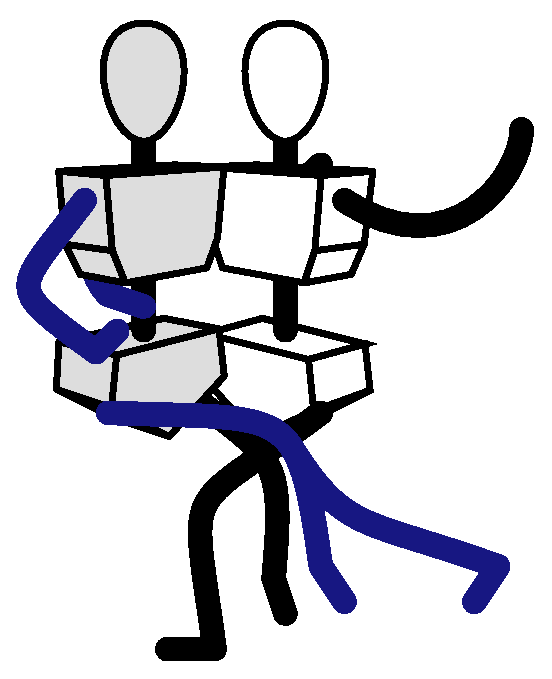
\includegraphics[width=0.23\textwidth]{chapters/cap-historia-passos/cadeirinha.eps}
  \caption{Pose final da  cadeirinha.}
  \label{fig:cadeirinhastickman}
  \vspace{-10pt}
\end{wrapfigure}
No \AnoLivro, o nome cadeirinha representa de forma particular a uma postura onde o \hyperref[def:Seguidor]{\textbf{seguidor}} 
senta-se sobre a perna do \hyperref[def:Condutor]{\textbf{condutor}}  (comumente sobre a perna esquerda);
por outro lado, de forma mais geral  o nome representa a qualquer movimento que tenha como final a 
\hyperref[def:cadeirinha-position]{\textbf{posição de cadeirinha}}.

A saída do chão do seguidor pode-se originar desde vários movimentos ou passos,
como por exemplo do  \hyperref[def:PassoBalao]{\textbf{balão}}; 
porem,
todos conservam a mesma técnica, que ao igual que  no caso do passo  \hyperref[def:PassoElevador]{\textbf{elevador}},
a suspensão no ar do seguidor, é mantida e sustentada pelo braço esquerdo do condutor,
que para este propósito  desce da linha dos ombros.
É importante lembrar que este braço não faz força para levantar ao seguidor, 
e sim simplesmente tenta manter a postura,
o que misturado com o movimento do corpo do condutor (esticar as pernas anteriormente flexionadas, principalmente)
provoca a saída do chão e suspensão do seguidor.
A Figura \ref{fig:cadeirinhastickman} mostra um desenho onde se observa a pose final da cadeirinha.


%%%%%%%%%%%%%%%%%%%%%%%%%%%%%%%%%%%%%%%%%%%%%%%%%%%%%%%%%%%%%%%%%%%%%%%%%%%%%%%
\subsection{Bicicleta}
\index{Passo!Bicicleta}

%%                CICLICO     |SIMETRICO      |CONTRATEMPO   |DESLOCAMENTOS |TIEMPOS
\caracterpasso{\NoCheckedItem}{\NoCheckedItem}{\NoCheckedItem}{\NoCheckedItem}{2}
Movimento sem data de criação conhecida \cite[pp. 143,144]{perna2002samba}.
Porem, podemos ver uma menção a este movimento, junto a outros conhecidos no samba de gafieira, 
em 1979 na revista ``Isto é'' \cite[pp. 89]{revista1979isto}.

No \AnoLivro, o nome bicicleta representa a um movimento da família das escovinhas,
especialmente emparentado com o tipo de escovinhas que chutam para atrás.
Uma vez entrado no movimento da bicicleta é possível pedalar (ou escovar) indefinidamente;
porem isto é pouco comum, na pratica é comum ver só 3 chutes (em 2 tempos) ou 5 chutes (em 3 tempos) ,
pelo que no movimento, mesmo tendo a possibilidade, 
não se executam as pedaladas ou escovadas da contraparte simétrica do primeiro grupo de 3 chutes,
que levariam a completar um ciclo;
pois isto obrigaria a alongar a duração do movimento a mais de 3 tempos,
o que jogaria em contra do espirito deste que é a surpresa.

Existem varias formas para chegar à posição inicial da bicicleta,  
a forma mais simples é a partir do \hyperref[def:abracodedanca]{\textbf{abraço de dança}},
estando o par, frente a frente, 
e com o peso do corpo no lado do pé esquerdo do \hyperref[def:Condutor]{\textbf{condutor}}.
Nesse momento, se o condutor é quem realizará a bicicleta, 
este leva o pé direito atrás,
deixando numa postura estática ao \hyperref[def:Seguidor]{\textbf{seguidor}} 
que servirá de apoio ou referencia;   
o condutor estará ligeiramente inclinado,
procurando ficar numa postura perpendicular entre os planos frontais de ambos dançarinos.
É nesse ponto que o condutor, escova 3 vesses para atrás iniciando com o pé direito,
no tempos 1, 1.5 e 2. No casos que sejam 5 escovadas, se chuta nos tempos,
1, 1.5, 2, 2.5 e 3. No final o condutor termina com o peso do corpo na perna direita,
e pode sair dessa postura, uma forma interessante é fazendo ambos uma tesoura.

%%%%%%%%%%%%%%%%%%%%%%%%%%%%%%%%%%%%%%%%%%%%%%%%%%%%%%%%%%%%%%%%%%%%%%%%%%%%%%%
%%%%%%%%%%%%%%%%%%%%%%%%%%%%%%%%%%%%%%%%%%%%%%%%%%%%%%%%%%%%%%%%%%%%%%%%%%%%%%%
\PRLsep{Passos no samba de gafieira anteriores a 1990}

%%%%%%%%%%%%%%%%%%%%%%%%%%%%%%%%%%%%%%%%%%%%%%%%%%%%%%%%%%%%%%%%%%%%%%%%%%%%%%%
\subsection{ Picadinho (Picadilho)}
\index{Passo!Picadilho}
\index{Passo!Picadinho}
\index{Passo cíclico!Picadinho}
\index{Passo simétrico!Picadinho}
\index{Passo de deslocamento!Picadinho}


Em palavras de Jimmy de Oliveira este movimento já existia antes de 1990 \cite{sambafunkeadoJimmyDeOliveiraPart1}.
Na década de 1920, podemos ver na revista ``A Cigarra'', 
referencias a um tipo de música e de dança denominado picadinho,
geralmente indicado com frases como \cite[pp. 13]{picadinho1}:
\begin{citando}
O chefe da turma é Zezé de Almeida, excellente pianista,
que nos entontece, quando toca os seus \textbf{picadinhos} apimentados;~\\
$[$...$]$~\\
é o Deco. Que rapasinho admiravel.. para dansar \textbf{picadinho}! 
Zezé tocando e Deco dansando, tenho eu divertimento 
para toda a vida e mais seis mezes.
\end{citando}
Em números posteriores da revista, 
podemos achar outras referencias ao picadinho como dança \cite[pp. 52]{picadinho2} \cite[pp. 49]{picadinho3}.


O picadilho ou picadinho, no \AnoLivro~ é um movimento de pouco deslocamento, 
se realiza com um abraço mais folgado, 
para dar espaço ao movimento do \hyperref[def:Seguidor]{\textbf{seguidor}}.
Cada ciclo do movimente dura 4 tempos, sendo o primeiro par de tempos do passo, simétrico ao segundo.

%%                CICLICO     |SIMETRICO   |CONTRATEMPO   |DESLOCAMENTOS |TIEMPOS
\caracterpasso{\CheckedItem}{\CheckedItem}{\NoCheckedItem}{\CheckedItem}{4}
Para uma correta execução do movimento, 
o \hyperref[def:Condutor]{\textbf{condutor}} envia informação de condução mediante o 
\hyperref[def:abracodedanca]{\textbf{abraço de dança}},
de modo que esta informação chegue quase sem degradação ate o quadril do seguidor,
é nesse ponto que a condução provoca o movimento das pernas (uma por vez), de modo que
o seguidor mantêm em todo momento as ``pernas fechadas''\footnote{
Ter as pernas fechadas, neste contexto, não indica literalmente ter as pernas juntas, 
e sim juntar as pernas como se em todo momento ao caminhar tentássemos segurar uma folha de papel na virilha.}.
Assim, na primeira metade do ciclo do passo, no tempo 1, o seguidor,
da inicialmente um passo ao frente ganhando o peso do corpo, 
logo no tempo 1.5 o pé livre que está atrás faz um movimento para fechar mais as pernas, 
ganhando este pé o peso do corpo; finalmente, o novo pé livre se movimenta ligeiramente ao frente no tempo 2, 
para ajeitar a postura e ganhar o peso do corpo, neste caso se descansa um tempo 2 completo.
A segunda metade do ciclo é similar à primeira e inicia no tempo 3, só que agora se começa com o outro pé, 
o pé livre do peso do corpo.


%%%%%%%%%%%%%%%%%%%%%%%%%%%%%%%%%%%%%%%%%%%%%%%%%%%%%%%%%%%%%%%%%%%%%%%%%%%%%%%
%%%%%%%%%%%%%%%%%%%%%%%%%%%%%%%%%%%%%%%%%%%%%%%%%%%%%%%%%%%%%%%%%%%%%%%%%%%%%%%
\PRLsep{Passos de samba de gafieira nas décadas 1980 e 1990}

%%%%%%%%%%%%%%%%%%%%%%%%%%%%%%%%%%%%%%%%%%%%%%%%%%%%%%%%%%%%%%%%%%%%%%%%%%%%%%%
\subsection{Caminhada a contratempo}
\index{Passo!Caminhada a contratempo}
\index{Passo cíclico!Caminhada a contratempo}
\index{Passo a contratempo!Caminhada a contratempo}
\index{Passo de deslocamento!Caminhada a contratempo}
%%                CICLICO     |SIMETRICO   |CONTRATEMPO   |DESLOCAMENTOS |TIEMPOS
\caracterpasso{\CheckedItem}{\NoCheckedItem}{\CheckedItem}{\CheckedItem}{3}
A caminhada a contratempo ou simplesmente caminhada é
uma passo que foi  criado\footnote{Marco Antonio Perna no seu livro 
``Samba de gafieira: A historia da dança de salão brasileira''
só indica o nome caminhada, que é ambíguo pois existem vários 
movimentos que podem ser chamados desse jeito; porém, no
DVD que vem adjunto ao livro e no canal de 
\href{https://www.youtube.com/watch?v=Bke_poU6NBc}{youtube} de Marco Antonio,
pode ser visto que a caminhada corresponde com o passo caminhada a contratempo.} 
entre o final da década de 1980 e inícios de 1990  \cite[pp. 143]{perna2002samba}.
A caminhada a contratempo, no \AnoLivro, 
é um \hyperref[def:PassoCiclico]{\textbf{passo cíclico}} e 
um movimento de deslocamento que dura 3 tempos;
este inicia e finaliza na \hyperref[def:X-position]{\textbf{posição de X}} e usa em todo momento 
um \hyperref[def:abracodedanca]{\textbf{abraço de dança}} na 
\hyperref[def:open-position]{\textbf{posição aberta}}.

Para atingir o tempo 1 o \hyperref[def:Condutor]{\textbf{condutor}} mexe a perna esquerda para adiante, 
e o \hyperref[def:Seguidor]{\textbf{seguidor}}  a direita para atrás,
chegando o par a uma \hyperref[def:frente-frente-position]{\textbf{posição frente a frente}}
com o peso do corpo do lado da perna esquerda do condutor.
Para atingir o tempo 1.5 o condutor cruza a perna direita atrás da esquerda,
e o seguidor a esquerda adiante da direita, levando o peso do corpo com este movimento.
Para atingir o tempo 2 o condutor mexe a perna esquerda, e o seguidor a direita,
descruzando suas pernas, seguindo o fluxo e direção do movimento,
chegando a uma \hyperref[def:frente-frente-position]{\textbf{posição frente a frente}}
com o peso do corpo do lado da perna esquerda do condutor.
Finalmente, para atingir o tempo 3 o condutor mexe a perna direita adiante da esquerda,
e o seguidor a esquerda atrás da direita, 
seguindo o fluxo e direção do movimento para chegar a uma posição de X. 

%%%%%%%%%%%%%%%%%%%%%%%%%%%%%%%%%%%%%%%%%%%%%%%%%%%%%%%%%%%%%%%%%%%%%%%%%%%%%%%
\begin{comment}
\subsection{\textcolor{blue}{Chicote}} 
\index{Passo!Chicote}
Este passo foi  criado entre o final da década de 1980 e inícios de 1990  \cite[pp. 143]{perna2002samba}.
\end{comment}

%%%%%%%%%%%%%%%%%%%%%%%%%%%%%%%%%%%%%%%%%%%%%%%%%%%%%%%%%%%%%%%%%%%%%%%%%%%%%%%
\subsection{\textcolor{blue}{Giro da dama}}
\index{Passo!Giro da dama}
Movimento criado por Jaime Arôxa, entre os anos de 1987 a 1990 \cite{EntrevistaJaimeAroxa1},
sendo este um movimento considerado de nível básico \cite[pp. 144]{perna2002samba}.


%%%%%%%%%%%%%%%%%%%%%%%%%%%%%%%%%%%%%%%%%%%%%%%%%%%%%%%%%%%%%%%%%%%%%%%%%%%%%%%
\subsection{\textcolor{blue}{Tirada de perna}}
\index{Passo!Tirada de perna}
Movimento criado por Jaime Arôxa, entre os anos de 1987 a 1990,
este movimento teve influencias das aulas de tango ditadas por Jaime \cite{EntrevistaJaimeAroxa1},
sendo este um movimento considerado de nível intermediaria \cite[pp. 144]{perna2002samba}.

%%%%%%%%%%%%%%%%%%%%%%%%%%%%%%%%%%%%%%%%%%%%%%%%%%%%%%%%%%%%%%%%%%%%%%%%%%%%%%%
\subsection{\textcolor{blue}{Esse}}
\index{Passo cíclico!Esse} 
\index{Passo!Esse}
Este passo foi  criado entre o final da década de 1980 e inícios de 1990  \cite[pp. 143]{perna2002samba}.

%%%%%%%%%%%%%%%%%%%%%%%%%%%%%%%%%%%%%%%%%%%%%%%%%%%%%%%%%%%%%%%%%%%%%%%%%%%%%%%
\subsection{Facão}
\label{subsec:desc:passo:facao}
\index{Passo!Facão}
\index{Posição!Posição de facão}
\index{Posição de finalização!Posição de facão}

%%                FINALIZA     |TRANSIÇÂO
\caracterpostura{\CheckedItem}{\NoCheckedItem}
Esta posição ou passo foi  criado entre o final da década de 1980 e inícios de 1990  \cite[pp. 143]{perna2002samba}.
Porem na década de 1950 existia um movimento que tinha um final semelhante a esta posição, 
este se chamava ``joelhada'' \cite[pp. 160]{fornaciari1950aprender};
porem, o abraço  não era colado,
e sim mais aberto de modo que o casal terminava tendo contato só nos joelhos.
Assim, a joelhada pode ter sido o precursor ou quem inspirou a criação do facão.

\begin{wrapfigure}{r}{0.25\textwidth}
  \vspace{-10pt}
  \centering
    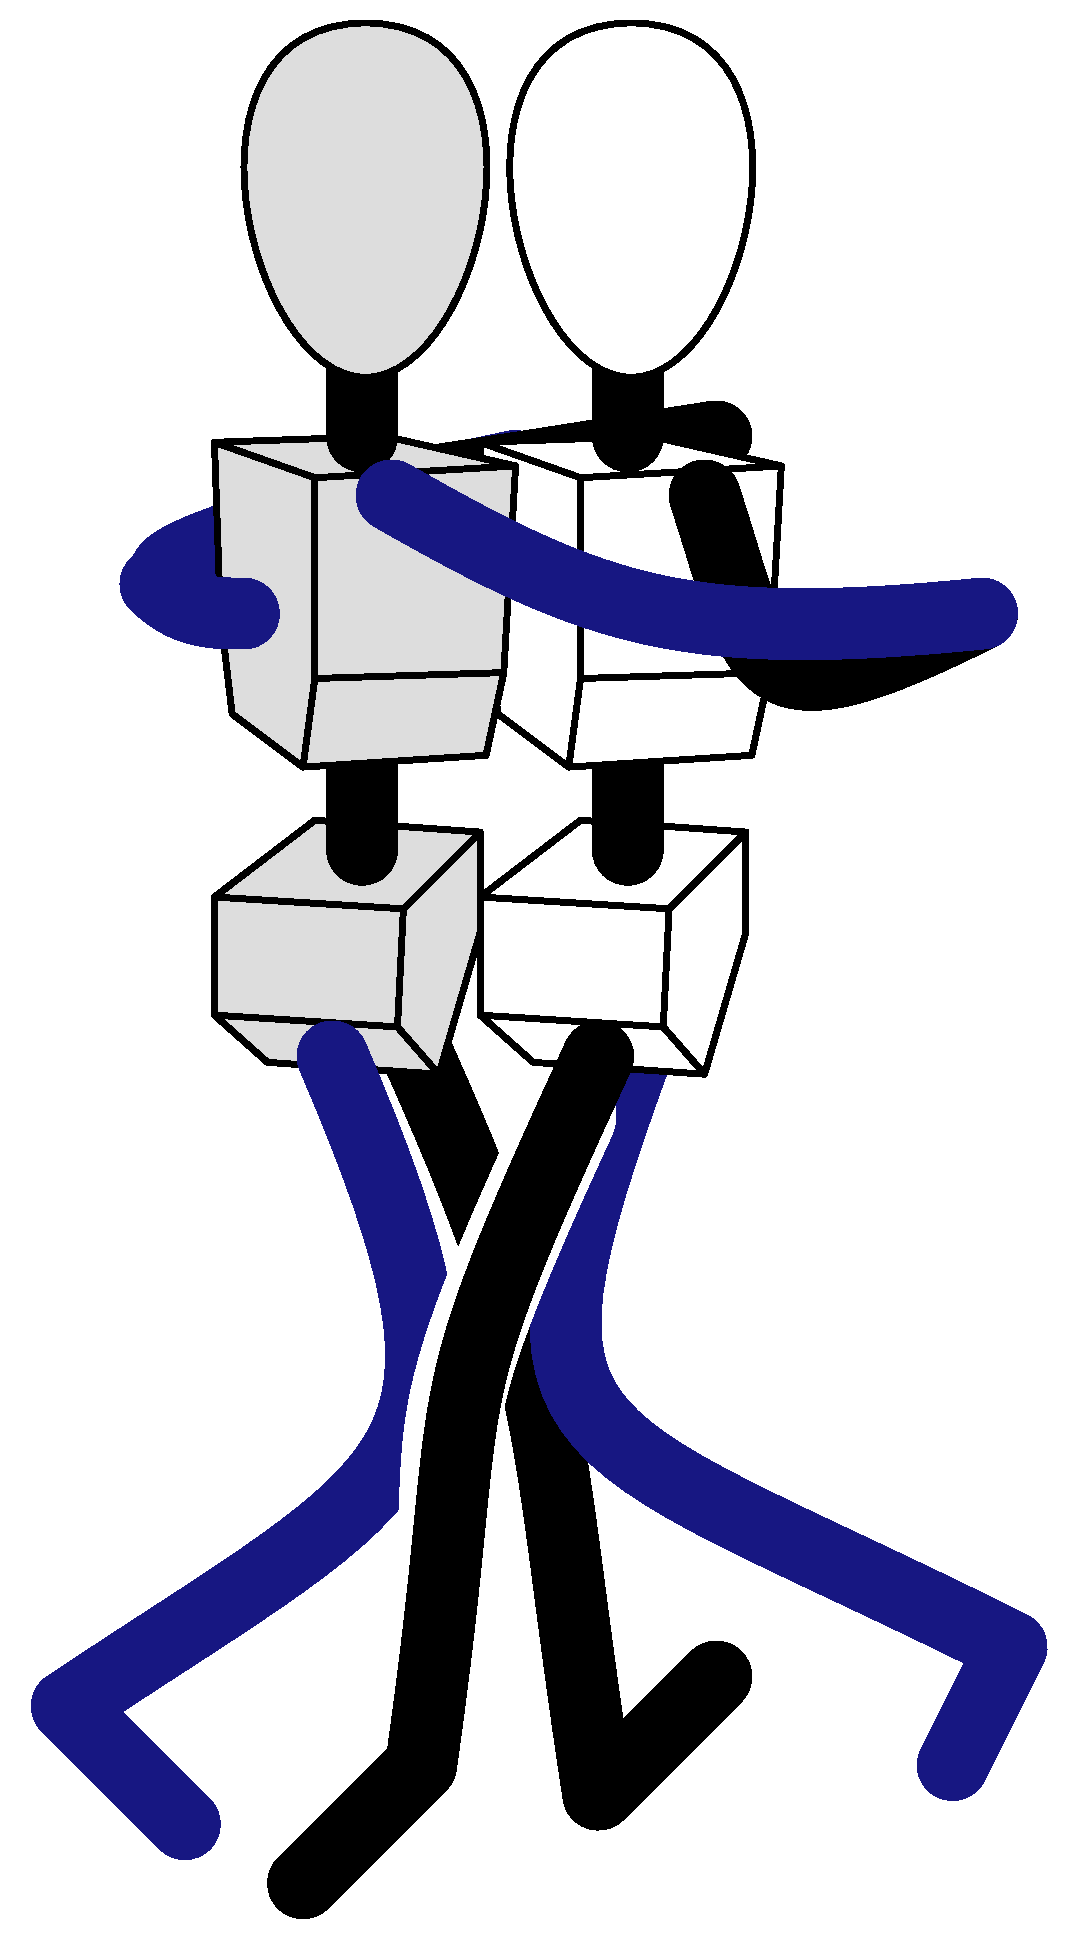
\includegraphics[width=0.23\textwidth]{chapters/cap-historia-passos/facao.eps}
  \caption{Pose final do facão.}
  \label{fig:facaostickman}
  \vspace{-10pt}
\end{wrapfigure}
Voltando ao facão de \AnoLivro, pessoalmente entendo mais este como uma posição que 
como um movimento ou passo. 
Isto é porque existem varias formas pra chegar à \hyperref[def:facao-position]{\textbf{posição de facão}},
de modo que é difícil apontar uma delas para assumir o nome de facão sobre as outras.

A posição do facão, é uma onde o par de dança está num abraçado colado e frente a frente, 
de modo que ambos tem a perna direita um pouco atrás do \hyperref[def:PlanoFrontal]{\textbf{plano frontal}} da linha da cabeça,
e a perna esquerda um pouco adiante no mesmo plano; com esta descrição se deduz 
que ambos tem o peso do corpo dividido em ambos pés; pelo que esta postura,
deve entende-se como uma de descanso, momentâneo porem descanso;
é dizer, se nossa dança fosse um relato escrito, a posição do facão
representaria um ponto, ou em alguns casos um ponto e virgula.
Se o que pretendemos representar é um ponto e virgula, 
é interessante não dividir o peso do corpo 50\% e 50\% em ambos pés,
e sim carregar o peso do corpo um pouco mais em um 
para poder liberar facilmente u outro pé para poder sair elegantemente da posição de facão.  

Sobre as formas de chegar a posição de facão, a continuação será descrita a forma mais simples,
porem não a mais interessante. Iniciamos desde o passo, frente-trás também chamado básico, 
ou básico linear no samba de gafieira. Desde o ponto de vista do \hyperref[def:Condutor]{\textbf{condutor}}, 
com um \hyperref[def:abracodedanca]{\textbf{abraço de dança}} colado,
damos primeiro duas pisadas no lugar, iniciando com a perna esquerda no tempo 1, e logo a perna direita no tempo 1.5,
logo damos um passo atrás com a perna direita no tempo 2; 
finalmente no tempo 3 damos mais um passo atrás com a perna direita, 
e se temos mantido o abraço colado, 
o \hyperref[def:Seguidor]{\textbf{seguidor}} sentirá a necessidade de dar um passo a frente com a perna esquerda,
chegando ambos à posição de facão.  

Este movimento linear para atrás e pouco interessante para chegar ao facão, mas pode ser apimentado,
se usamos um movimento sinuoso para atrás (em vez de um linear), este movimento,
é promovido pelo condutor, e tem forma de ``S'' onde a ligeira curva para a esquerda é realizada no tempo 1 e 1.5,
no tempo  2 chegamos ao ponto neutro o meio, onde a curva esta sobre a linha reta, e para chegar a 3, 
que também está sobre a linha reta e ao final de ambas curvas,
o condutor promove a curva para a sua direita.

%%%%%%%%%%%%%%%%%%%%%%%%%%%%%%%%%%%%%%%%%%%%%%%%%%%%%%%%%%%%%%%%%%%%%%%%%%%%%%%
\subsection{Faquinha}
\index{Passo!Faquinha}
\index{Passo de deslocamento!Faquinha}
\index{Passo cíclico!Faquinha}
%%                CICLICO     |SIMETRICO   |CONTRATEMPO   |DESLOCAMENTOS |TIEMPOS
\caracterpasso{\CheckedItem}{\NoCheckedItem}{\NoCheckedItem}{\CheckedItem}{2}
Este passo foi  criado entre o final da década de 1980 e inícios de 1990  \cite[pp. 143]{perna2002samba}.
É uma variante do  \hyperref[subsec:desc:passo:facao]{\textbf{facão}} (passo), 
com a diferencia que o movimento tem uma posição final (facão) menos acentuada;
sendo mais parecido a um casal num \hyperref[def:abracodedanca]{\textbf{abraço de dança}} colado, 
na \hyperref[def:frente-frente-position]{\textbf{posição frente a frente}}  e com uma perna ligeiramente adiantada a outra;
com diferencia da \hyperref[def:facao-position]{\textbf{posição de facão}}, 
onde as pernas tem uma separação que claramente evidencia uma posição do descanso;
a faquinha, pelo contrario, termina numa posição final de transição, 
pois comumente são realizadas varias faquinhas de forma consecutiva antes de realizar um facão,
 para assim finalizar a sequencia de forma mais acentuada.

O passo faquinha dura dois tempos, e consta de dois movimentos, 
onde a posição final é igual à inicial de modo que o passo pode repetir-se ciclicamente indefinidamente.
O movimento inicia quando o par de dança está numa posição de facão pouco acentuada;
é dizer, quando cada um tem pouca separação entre os pés; 
e o peso do corpo está do lado da perna direita do \hyperref[def:Condutor]{\textbf{condutor}}.
Logo, no primeiro tempo, 
o condutor junta os pés trazendo sua pé esquerdo junto à direito e trocando o peso do corpo a esse pé,
mantendo o abraço para provocar um movimento simétrico no \hyperref[def:Seguidor]{\textbf{seguidor}};
porem a ação do movimento dos pés não é uma causa e sim um efeito,
pois é provocado por uma condução do tórax usando que é transmitida por médio do abraço colado;
para isto o condutor gira o tórax no sentido horário no \hyperref[def:PlanoAxial]{\textbf{plano axial}},
tentando suspender ligeiramente o corpo do seguidor e o seu próprio.
No segundo tempo, o condutor dá um passo atrás com sua perna direita,
 mantendo o abraço colado e provocando que o seguidor de um passo adiante com sua perna esquerda,
chegando novamente a posição inicial.



%%%%%%%%%%%%%%%%%%%%%%%%%%%%%%%%%%%%%%%%%%%%%%%%%%%%%%%%%%%%%%%%%%%%%%%%%%%%%%%
\subsection{\textcolor{blue}{Gancho}} 
\index{Passo!Gancho}
Este passo foi  criado entre o final da década de 1980 e inícios de 1990  \cite[pp. 143]{perna2002samba}.

%%%%%%%%%%%%%%%%%%%%%%%%%%%%%%%%%%%%%%%%%%%%%%%%%%%%%%%%%%%%%%%%%%%%%%%%%%%%%%%
\subsection{\textcolor{blue}{Gancho redondo}} 
\index{Passo!Gancho redondo}
Este passo foi  criado entre o final da década de 1980 e inícios de 1990  \cite[pp. 143]{perna2002samba}.

%%%%%%%%%%%%%%%%%%%%%%%%%%%%%%%%%%%%%%%%%%%%%%%%%%%%%%%%%%%%%%%%%%%%%%%%%%%%%%%
\subsection{\textcolor{blue}{Letra}}
\index{Passo!Letra}
Este passo foi  criado entre o final da década de 1980 e inícios de 1990  \cite[pp. 143]{perna2002samba}.

%%%%%%%%%%%%%%%%%%%%%%%%%%%%%%%%%%%%%%%%%%%%%%%%%%%%%%%%%%%%%%%%%%%%%%%%%%%%%%%
\subsection{\textcolor{blue}{Puladinho redondo}} 
\index{Passo!Puladinho redondo}
Este passo foi  criado entre o final da década de 1980 e inícios de 1990  \cite[pp. 143]{perna2002samba}.

%%%%%%%%%%%%%%%%%%%%%%%%%%%%%%%%%%%%%%%%%%%%%%%%%%%%%%%%%%%%%%%%%%%%%%%%%%%%%%%
\subsection{\textcolor{blue}{Trança}}
\index{Passo cíclico!Trança}
\index{Passo!Trança}
Este movimento é antigo, porem Jaime Arôxa trabalhou sobre ele entre os anos de 1987 a 1990,
pois não existia uma didática para o ensino do movimento, 
e era realizado apenas pelos homens; 
de modo que Jaime agregou a parte do seguidor no par de dança  \cite{EntrevistaJaimeAroxa1} \cite[pp. 143]{perna2002samba}.
%%%%%%%%%%%%%%%%%%%%%%%%%%%%%%%%%%%%%%%%%%%%%%%%%%%%%%%%%%%%%%%%%%%%%%%%%%%%%%%
\subsection{\textcolor{blue}{Tesoura}}
\index{Passo!Tesoura}
Movimento criado por Jaime Arôxa, entre os anos de 1987 a 1990 \cite{EntrevistaJaimeAroxa1} \cite[pp. 143]{perna2002samba}.

%%%%%%%%%%%%%%%%%%%%%%%%%%%%%%%%%%%%%%%%%%%%%%%%%%%%%%%%%%%%%%%%%%%%%%%%%%%%%%%
%%%%%%%%%%%%%%%%%%%%%%%%%%%%%%%%%%%%%%%%%%%%%%%%%%%%%%%%%%%%%%%%%%%%%%%%%%%%%%%
\PRLsep{Passos de samba de gafieira da décadas de 1990}

%%%%%%%%%%%%%%%%%%%%%%%%%%%%%%%%%%%%%%%%%%%%%%%%%%%%%%%%%%%%%%%%%%%%%%%%%%%%%%%
\subsection{\textcolor{blue}{Assalto}} 
\index{Passo!Assalto}
\index{Passo cíclico!Assalto}
Este passo foi criado por Jimmy de Oliveira apos o ano 1990 \cite{sambafunkeadoJimmyDeOliveiraPart1}.

%%%%%%%%%%%%%%%%%%%%%%%%%%%%%%%%%%%%%%%%%%%%%%%%%%%%%%%%%%%%%%%%%%%%%%%%%%%%%%%
\subsection{\textcolor{blue}{Boneca}} 
\index{Passo!Boneca}
Este passo foi criado por Jimmy de Oliveira apos o ano 1990 \cite{sambafunkeadoJimmyDeOliveiraPart1}.

%%%%%%%%%%%%%%%%%%%%%%%%%%%%%%%%%%%%%%%%%%%%%%%%%%%%%%%%%%%%%%%%%%%%%%%%%%%%%%%
\subsection{\textcolor{blue}{Elástico}} 
\index{Passo!Elastico}
Este passo foi criado por Jimmy de Oliveira apos o ano 1990 \cite{sambafunkeadoJimmyDeOliveiraPart1}.

%%%%%%%%%%%%%%%%%%%%%%%%%%%%%%%%%%%%%%%%%%%%%%%%%%%%%%%%%%%%%%%%%%%%%%%%%%%%%%%
\subsection{\textcolor{blue}{Escovinha}}
\index{Passo cíclico!Escovinha}
\index{Passo!Escovinha}
Este passo foi criado por Jimmy de Oliveira apos o ano 1990 \cite{sambafunkeadoJimmyDeOliveiraPart1}.

%%%%%%%%%%%%%%%%%%%%%%%%%%%%%%%%%%%%%%%%%%%%%%%%%%%%%%%%%%%%%%%%%%%%%%%%%%%%%%%
\begin{comment}
\subsection{Homem na lua}
Este passo foi criado por Jimmy de Oliveira apos o ano 1990 \cite{sambafunkeadoJimmyDeOliveiraPart1}.
\end{comment}

%%%%%%%%%%%%%%%%%%%%%%%%%%%%%%%%%%%%%%%%%%%%%%%%%%%%%%%%%%%%%%%%%%%%%%%%%%%%%%%
\subsection{\textcolor{blue}{Pescaria}} 
\index{Passo!Pescaria}
Este passo foi criado por Jimmy de Oliveira apos o ano 1990 \cite{sambafunkeadoJimmyDeOliveiraPart1}.

%%%%%%%%%%%%%%%%%%%%%%%%%%%%%%%%%%%%%%%%%%%%%%%%%%%%%%%%%%%%%%%%%%%%%%%%%%%%%%%
\subsection{\textcolor{blue}{Romário}}
\label{subsec:passo:romario}
\index{Passo cíclico!Romário} 
\index{Passo!Romário}
Este passo foi criado por Jimmy de Oliveira apos o ano 1990 \cite{sambafunkeadoJimmyDeOliveiraPart1}.


%%%%%%%%%%%%%%%%%%%%%%%%%%%%%%%%%%%%%%%%%%%%%%%%%%%%%%%%%%%%%%%%%%%%%%%%%%%%%%%
%%%%%%%%%%%%%%%%%%%%%%%%%%%%%%%%%%%%%%%%%%%%%%%%%%%%%%%%%%%%%%%%%%%%%%%%%%%%%%%
\PRLsep{Passos de samba de gafieira sem data conhecida}



%%%%%%%%%%%%%%%%%%%%%%%%%%%%%%%%%%%%%%%%%%%%%%%%%%%%%%%%%%%%%%%%%%%%%%%%%%%%%%%
\subsection{\textcolor{blue}{Balanço}}
\index{Passo!Balanço}
\index{Passo cíclico!Balanço}
Movimento sem data de criação conhecida, 
seguindo Jaime Arôxa o balanço sempre existiu desde do início do século, 
no maxixe \cite{EntrevistaJaimeAroxa1},
sendo este um movimento considerado de nível básico \cite[pp. 144]{perna2002samba}.


%%%%%%%%%%%%%%%%%%%%%%%%%%%%%%%%%%%%%%%%%%%%%%%%%%%%%%%%%%%%%%%%%%%%%%%%%%%%%%%
\subsection{\textcolor{blue}{Saída lateral}}
\index{Passo!Saída lateral}
Movimento sem data de criação conhecida,
sendo este um movimento considerado de nível básico \cite[pp. 144]{perna2002samba}.

%%%%%%%%%%%%%%%%%%%%%%%%%%%%%%%%%%%%%%%%%%%%%%%%%%%%%%%%%%%%%%%%%%%%%%%%%%%%%%%
\subsection{\textcolor{blue}{Tirada ao lado}}
\index{Passo!Tirada ao lado}
Movimento sem data de criação conhecida,
sendo este um movimento considerado de nível básico \cite[pp. 144]{perna2002samba}.

%%%%%%%%%%%%%%%%%%%%%%%%%%%%%%%%%%%%%%%%%%%%%%%%%%%%%%%%%%%%%%%%%%%%%%%%%%%%%%%
\begin{comment}
\subsection{\textcolor{blue}{Mestre sala}}
\index{Passo!Mestre sala}
Movimento sem data de criação conhecida \cite[pp. 144]{perna2002samba}.
\end{comment}


%%%%%%%%%%%%%%%%%%%%%%%%%%%%%%%%%%%%%%%%%%%%%%%%%%%%%%%%%%%%%%%%%%%%%%%%%%%%%%%
\begin{comment}
\subsection{\textcolor{blue}{Enceradeira}}
\index{Passo!Enceradeira}
Movimento sem data de criação conhecida \cite[pp. 144]{perna2002samba}.
\end{comment}



%%%%%%%%%%%%%%%%%%%%%%%%%%%%%%%%%%%%%%%%%%%%%%%%%%%%%%%%%%%%%%%%%%%%%%%%%%%%%%%
%%%%%%%%%%%%%%%%%%%%%%%%%%%%%%%%%%%%%%%%%%%%%%%%%%%%%%%%%%%%%%%%%%%%%%%%%%%%%%%

\begin{comment}
Passos acrobáticos ou para apresentações \cite[pp. 142-143]{perna2002samba}:
\begin{tasks}
\task \textbf{Cabide}, \index{Passo!Cabide} oriundo do rock.
\task \textbf{Baratinha} \index{Passo!Baratinha}
\task \textbf{Enceradeira}, \index{Passo!Enceradeira} criado em algum momento no final da década de 1980 e inícios da década de 1990.
\end{tasks}
\end{comment}

\newpage
%%%%%%%%%%%%%%%%%%%%%%%%%%%%%%%%%%%%%%%%%%%%%%%%%%%%%%%%%%%%%%%%%%%%%%%%%%%%%%%
%%%%%%%%%%%%%%%%%%%%%%%%%%%%%%%%%%%%%%%%%%%%%%%%%%%%%%%%%%%%%%%%%%%%%%%%%%%%%%%
%%%%%%%%%%%%%%%%%%%%%%%%%%%%%%%%%%%%%%%%%%%%%%%%%%%%%%%%%%%%%%%%%%%%%%%%%%%%%%%
\section{Sobre o $syllabus$ do samba de gafieira}

O $syllabus$  do samba de gafieira, foi criado no ano 2001 em Rio de Janeiro,
este é um listado de passos ordenado em três níveis (básico, intermediário e avançado),
selecionados por votação,
onde são agrupados passos que se consideram essenciais para o ensino e competição;
neste listado não entram passos aéreos \cite[pp. 144]{perna2002samba}.


As personas que participaram da votação para a elaboração do $syllabus$ são \cite[pp. 144]{perna2002samba}:
\begin{inparaitem}[$*$]
\item Bob Cunha e Aurya
\item Bolacha
\item Bruno Barros
\item Carlinhos de Jesus
\item Dani Aguiar
\item Dani Escudero
\item Dani Galper
\item Egídio
\item Flávio Miguel
\item Gérson Reis
\item Kilve
\item Luis Florião/Adriana
\item Marcello Moragas
\item Marco Antonio Perna
\item Marquinhos Copacabana
\item Rogério Mendonça
\item Valdeci
\item Wanir Almeida
\end{inparaitem}.\\



Os passos de \textbf{nível básico} são:
\begin{tasks}(2)
\task Básico (frente-trás)
\task Balanço 
\task Caminhada (ou caminhada a contratempo)
\task Cruzado
\task Esse
\task Gancho
\task Giro da dama
\task Puladinho
\task Saída lateral
\task Tirada ao lado
\end{tasks}~\\


Os passos de \textbf{nível intermediário} são:
\begin{tasks}(2)
\task Assalto
\task Balão apagado
\task Escovinha
\task Facão
\task Gancho redondo
\task Mestre sala
\task Romário
\task Tesoura
\task Tirada de perna
\task Trança
\end{tasks}~\\

Os passos de \textbf{nível avançado} são:
\begin{tasks}(2)
\task Bicicleta
\task Enceradeira
\task Pião
\task Picadinho (ou ou picadilho)
\task Pica-pau
\end{tasks}



\index{Dicionario do samba de gafieira}
\begin{figure}[t]
\begin{elaboracion}[title=Necessidade e alternativas ao Syllabus]

Para o idioma espanhol existe\footnote{\url{https://www.rae.es/la-institucion}} a ``Real Academia Espanhola'' (RAE),
que ``é uma instituição com personalidade jurídica própria, cuja principal missão é garantir 
que as mudanças sofridas pela língua espanhola, 
em sua constante adaptação às necessidades do seus falantes, 
não quebrem a unidade essencial que ela mantém em toda a esfera hispânica".
Nesse sentido a RAE leva registro da língua mediante um \textbf{dicionario},
cuja função é recolher o uso atual da língua, dar um marco comum de comunicação aos falantes de espanhol,
e agregar em suas novas versões, novas palavras ou acepções;
tendo assim um papel de historiador ou cronista e não de regulador estrito do idioma.

Assim, minha opinião pessoal é que para evitar a desconfiança, que alguns profissionais da dança tem,
sobre a instituição de um Syllabus, no sentido  que poderia diminuir a força criativa do samba de gafieira;
podemos em vez instituir, por exemplo, mediante um ``\textbf{Conselho nacional do samba de gafieira}'',
um ``\textbf{Dicionario do samba de gafieira}'', que recolha de forma similar ao Syllabus,
um listado e descrição dos passos mais representativos para a data da liberação de cada edição do dicionario, 
ordenado eles em três níveis (básico, intermediário e avançado) 
com todas as acepções\footnote{Nomes diferentes para um mesmo movimento.}
e outros dados relativos ao samba de gafieira.
De modo que se leve um registro a traves do tempo de como evoluem os movimentos e nomes no samba de gafieira,
e no futuro se alguém o desejar, possa fazer mineração de dados e ver 
por exemplo, como era executado\footnote{Se alguém tem esta curiosidade,
porem para o ano de 1947, a duvida pode ser resolvida no livro
``Como aprender a dançar: novo método de danças modernas'' escrito por Gino Fornaciari \cite[pp. 72]{fornaciari1947aprender}.} 
o movimento que no \AnoLivro~era chamado de ``Pião''.
\end{elaboracion}
\label{fig:ImportanciaSyllabus}
\end{figure}






%----------------------------------------------------------------------------------------
%----------------------------------------------------------------------------------------
%----------------------------------------------------------------------------------------
%	PART
%----------------------------------------------------------------------------------------
\part{Musicalização para a dança de salão}

\chapterimage{chapter_head_teclado.pdf} % Chapter heading image

\chapter{Fundamentos de notação musical}
\label{cap:musicabasica}
Nas seguintes sub seções abordaremos alguns conceitos de notação musical;
porém, não aprofundaremos demasiado em toda a teoria musical, 
devido a que as explicações mostradas aqui, estão
orientadas para um público interessado na dança, que numa primeira 
aproximação à música, precisa conhecer rapidamente conceitos básicos. 
Mas, empoderamos a curiosidade de todos os leitores a aprofundar mais nestos temas, 
para este efeito existem na literatura muitos materiais, livros ou revistas especializadas 
\cite{medteoria}        %% Teoria Da Musica
\cite{cardoso1973curso} %% Curso Completo De Teoria Musical E Solfejo - 1o Vol.
\cite{mascarenhascurso} %% Curso Completo De Teoria Musical E Solfejo - 2o Vol.
\cite{grabner2001teoria}%% Teoría general de la música 
\cite{alves2004teoria}  %% teoria musical lições essenciais
\cite{apel1969harvard}  %% harvard diccionario
\cite{azevedocompor}    %% Como Compor Música Facilmente: métodos ou estudos para teoria, canto e solfejo (NOPDF)
\cite{adolfo2002musica}.%% Musica: Leitura, Conceitos, Exercicios (NOPDF)

%%%%%%%%%%%%%%%%%%%%%%%%%%%%%%%%%%%%%%%%%%%%%%%%%%%%%%%%%%%%%%%%%%%%%%%%%%%%%%%%

%%%%%%%%%%%%%%%%%%%%%%%%%%%%%%%%%%%%%%%%%%%%%%%%%%%%%%%%%%%%%%%%%%%%%%%%%%%%%%%%
\section{Componentes da música}

A música; na sua forma mais básica,  é um conjunto de sons; esta é criada ao combinar na justa medida: 
ingênio, técnica e arte.

Entre as características de um som temos \cite[pp. 12]{medteoria} :
\begin{description}
\item [Altura:] \label{sec:pos:Altura} 
Também chamado \textbf{tom}\footnote{A palavra tom tem vários significados em música, 
outro significado pode ser um intervalo ou distancia em frequência, 
utilizado na escala diatônica, para mais detalhes ir a Seção \ref{sec:notasmusicais}}, representa a frequência de vibração (principal) da onda mecânica que gera o sonido.
Isto é, que terão um altura maior os sonidos com maior frequência de vibração mecânica (mais agudos), 
e uma altura menor sonidos mais graves.
\begin{example}
A campainha pra chamar ao atendente de um hotel tem uma altura maior,
que a campana da igreja, que é tocada ao médio dia, que tem um sonido mais grave.
\end{example} 
\index{Altura}\index{Tom}
\item [Duração:] \label{sec:pos:Duracion}
Representa a longitude temporal, durante o qual um sonido será executado.
\begin{example}
Podemos assoviar durante um tempo, curto, longo, muito longo, etc.
\end{example} 
\index{Duração}
\item [Intensidade:] \label{sec:pos:Intensidade}
Se refere ao volume sonoro ou à potencia do sonido executado, 
de modo que o som pode ter intensidades, por exemplo: fracas, fortes, muito fortes, etc.  
\begin{example}
Si escolhemos dois pedaços de madeira e batimos eles um contra outro, 
podemos gerar sons com diferente intensidade, dependendo da força com que realizemos os batimentos.
\end{example} 
\index{Intensidade}
\item [Timbre:] \label{sec:pos:timbre}
Na definição da altura de um som, referenciamos esta seguindo a sua frequência principal,
porem um som não está composto exclusivamente por vibrações a esta frequência.
Na pratica os sons contem muitas outras frequências de vibração, acontecendo simultaneamente e 
que se manifestam com menor intensidade.
A combinação de todas estas frequências de vibração é o que gera o som que escutamos;
assim, a essa especifica configuração de frequências a chamamos como o timbre ou
a ``\textbf{cor}'' do som.
\begin{example}
Se geramos dois sonidos com a mesma altura; mas, um sonido executado por uma flauta,
e o outro por um violão, ambos sonidos terão diferentes timbres ou cores.
\end{example} 
\index{Timbre}
\end{description}
~\\

Conhecidas estas definições básicas, e procurando estruturas mais complexas na música,
podemos distinguir alguns componentes com que esta é constituída, 
por exemplo temos:

\begin{description}
\item [Ritmo:] \label{sec:pos:Ritmo}
Se refere a distribuição temporal da execução dos sonidos e a proporção na duração destes. 
Asim, o ritmo carateriza a música no âmbito temporal \cite[pp. 11]{medteoria}.
\index{Ritmo}
\begin{example}
Batendo palmas, criamos a sequencia de sonidos: palmas, pausa curta, palmas, palmas, pausa loga e palmas.
\end{example} 
\item [Melodia:] \label{sec:pos:Melodia}
É um conjunto de sons, que podem ter diferentes \hyperref[sec:pos:Altura]{\textbf{alturas}}, 
e que estão dispostos sequencialmente. 
A melodia representa um elemento horizontal\footnote{\label{eixohor}Eixo com múltiplas distribuições de tempo dos sons na música} na musica, 
e esta é indivisível do ritmo \cite[pp. 517]{apel1969harvard} \cite[pp. 11]{medteoria}.
\begin{example}
Se assoviamos ``parabéns pra você'', estamos executando uma melodia 
(executando diferentes sons numa distribuição temporal especifica).
\end{example} 
\index{Melodia} 
\item [Harmonia:] \label{sec:pos:Harmonia}
Conjunto de sons dispostos simultaneamente em \hyperref[sec:pos:Altura]{\textbf{alturas}} diferentes.
A harmonia representa um elemento vertical\footnote{\label{eixover}Eixo com múltiplas distribuições de frequência dos sons na música} na música \cite[pp. 371]{apel1969harvard} \cite[pp. 8]{cardoso1973curso} \cite[pp. 11]{medteoria}. 
\begin{example}
Se num piano pressionamos simultaneamente as teclas: Do, Mi e Sol. Estamos executando uma harmonia.
\end{example} 
\index{Harmonia} 
\item [Contraponto:] \label{sec:pos:Contraponto}
O termo deriva de ``punctus contra punctum'' que significa ``nota contra nota'', 
e por extensão ``melodia contra melodia''. 
Assim, falar de contraponto é equivalente a dizer, dois ou mais melodias executadas simultaneamente  
(concepção horizontal\footref{eixohor} e vertical\footref{eixover} da música)  \cite[pp. 208]{apel1969harvard} \cite[pp. 11]{medteoria}.
\begin{example}
Uma orquestra com vários músicos tocando cada um uma melodia.
\end{example} 
\index{Contraponto}
\end{description}


 
%%%%%%%%%%%%%%%%%%%%%%%%%%%%%%%%%%%%%%%%%%%%%%%%%%%%%%%%%%%%%%%%%%%%%%%%%%%%%%%%
\section{Figuras musicais, pausas e durações}
\index{Música!Figuras musicais}
\index{Música!Figuras rítmicas}
\label{sec:figurasmusicais}
As figuras musicais também chamada figuras rítmicas \cite[pp. 16]{alves2004teoria}, 
são um conjunto de sinais (desenhos), criadas pra indicar a relação 
entre as \hyperref[sec:pos:Duracion]{\textbf{durações}} dos sons \cite[pp. 20]{medteoria}.
Assim, podemos ver na coluna dois da Tabela \ref{tab:abc-noteslengthbasic}
 um conjunto de 6 destas figuras musicais; 
a primeira coluna representa a longitude temporal (\hyperref[sec:pos:Duracion]{\textbf{duração}}) de cada uma destas figuras;
porém, todos estas durações são relativas ao valor temporal $S$, em segundos, de uma figura \Ganz.
A terceira coluna da tabela contem os nomes de cada uma destas figuras musicais. 
\begin{table}[h]
\centering
\begin{tabular}{|c||c|c||c|c|}
\hline
Duração & Figura & Nome de figura & Pausa & Nome de pausa\\ \hline
\hline
$S$    & \Ganz   & Semibreve    & \GaPa  & Pausa de Semibreve \\ \hline
$S/2$  & \Halb   & Mínima       & \HaPa  & Pausa de Mínima \\ \hline
$S/4$  & \Vier   & Semínima     & \ViPa  & Pausa de Semínima \\ \hline
$S/8$  & \Acht   & Colcheia     & \AcPa  & Pausa de Colcheia \\ \hline
$S/16$ & \Sech   & Semicolcheia & \SePa  & Pausa de Semicolcheia \\ \hline
$S/32$ & \Zwdr   & Fusa         & \ZwPa  & Pausa de fusa  \\ \hline  
\end{tabular}
\caption{Duração e símbolos de algumas figuras musicais}
\label{tab:abc-noteslengthbasic}
\end{table}


\begin{example}
Se decidimos criar uma sequencia rítmica assoviando um único tom, porém
distribuindo os tempos de duração como: Longo, curto, curto; 
repetindo esta sequencia quatro vesses. 
Poderíamos escrever esta sequencia usando figuras musicais numa representação como a mostrada na Figura \ref{fig:abc-figurasexample1}.
É importante ressaltar que assumimos que  um sonido longo dura no tempo exatamente o dobro que um curto, 
e que decidimos\footnote{É escolhida uma semínima porém pode ter sido escolhida 
qualquer outra figura, dado que o valor $S$ não está definido.}
representar um sonido de longa duração como uma semínima.

Para entender melhor a representação com figuras musicais, 
podemos ir a uma representação alternativa com um gráfico da potencia sonora na execução dos sons,
como é representado na Figura \ref{fig:forma-figurasexample1b}.
É fácil perceber como a potencia do som se mantêm, ate justo antes de iniciar 
o seguinte som, de modo que não existem silêncios na sequencia rítmica.
\end{example} 




\begin{figure}[h]
    \centering
    \begin{subfigure}[b]{0.9\textwidth}
 \begin{abc}[name=abc-figurasexample1]
% abcm2ps figurasexample1.abc  -O figurasexample1.ps
% ps2epsi figurasexample1.ps figurasexample1.eps
%
X: 1 % start of header
K: none stafflines=0 %K: C %% Escala de C mayor %
M:  none % M: 2/4
%T: Contratempo num compasso binário
V:1 clef=none stem=up %name="Ritmo 1"   sname="Ritmo 1"
%
[V:1] | B2 B1 B1 B2 B1 B1 B2 B1 B1 B2  B1 B1   |
%       
\end{abc}
	\caption{Sequencia rítmica usando semínimas e colcheias.}
	\label{fig:abc-figurasexample1}
    \end{subfigure}
    ~%add desired spacing between images, e. g. ~, \quad, \qquad, \hfill etc. 
      %(or a blank line to force the subfigure onto a new line)
    \begin{subfigure}[b]{0.9\textwidth}
        \includegraphics[width=\textwidth]{chapters/cap-musica-basica/forma-figurasexample1.eps}
        \caption{Sequencia rítmica usando um gráfico indicando a potencia do sonido.}
        \label{fig:forma-figurasexample1b}
    \end{subfigure}
    \caption{Sequencia rítmica.}\label{fig:total-figurasexample1}
\end{figure}


Por outro lado, assim como a duração do tempo de execução de cada som precisa uma grafia,
os silêncios ou pausas, também precisam ser indicados. 
De modo que, para cada figura musical existe uma grafia que indica um silencio da mesma duração temporal,
como pode ser visto na quarta coluna da Tabela \ref{tab:abc-noteslengthbasic}.
O nome de cada uma destas pausas está descrito na quinta coluna da mesma tabela.

\begin{example}
Similarmente ao exemplo anterior, se decidimos criar uma sequencia rítmica assoviando um único tom, porém
intercalando sons e silêncios, criaremos um padrão rítmico como na Figura \ref{fig:total-figurasexample2}.

Podemos entender melhor a representação com figuras musicais, 
usando a representação com um gráfico da potencia sonora na execução dos sons,
como é representado na Figura \ref{fig:forma-figurasexample2}.
Nela percebemos como a potencia do som se mantêm durante a longitude de tempo estipulada pela figura musical, 
ate justo antes de iniciar o silencio, indicado por uma linha reta horizontal.
\end{example} 

\begin{figure}[h]
    \centering
    \begin{subfigure}[b]{0.9\textwidth}
 \begin{abc}[name=abc-figurasexample2]
% abcm2ps figurasexample2.abc  -O figurasexample2.ps
% ps2epsi figurasexample2.ps figurasexample2.eps
%
X: 1 % start of header
K: none stafflines=0 %K: C %% Escala de C mayor %
M:  none % M: 2/4
%T: Contratempo num compasso binário
V:1 clef=none stem=up %name="Ritmo 1"   sname="Ritmo 1"
%
[V:1] | z1 B1 z1 B1 z2 B1 z1 B1 z1 B1 z2 B1  z1 B1   |
%       
\end{abc}
	\caption{Sequencia rítmica usando  colcheias e silencios.}
	\label{fig:abc-figurasexample2}
    \end{subfigure}
    ~%add desired spacing between images, e. g. ~, \quad, \qquad, \hfill etc. 
      %(or a blank line to force the subfigure onto a new line)
    \begin{subfigure}[b]{0.9\textwidth}
        \includegraphics[width=\textwidth]{chapters/cap-musica-basica/forma-figurasexample2.eps}
        \caption{Sequencia rítmica usando um gráfico indicando a potencia do sonido.}
        \label{fig:forma-figurasexample2}
    \end{subfigure}
    \caption{Sequencia rítmica.}\label{fig:total-figurasexample2}
\end{figure}


Ate agora todos os exemplos foram sequencias rítmicas, 
pois não exploramos a possibilidade de variar a altura dos sons;
para poder explorar esta possibilidade devemos ter claro o conceito de pauta,
para que cada figura musical, 
além de nos proporcionar uma informação da \hyperref[sec:pos:Duracion]{\textbf{duração}}  dos sons, 
também nos de informação da \hyperref[sec:pos:Altura]{\textbf{altura}}  destes. 
Tendo estes dois fatores, altura e duração, podemos criar \hyperref[sec:pos:Melodia]{\textbf{melodias}}.

\begin{tcbattention}
O mistério de como distinguir a pausa de mínima (\HaPa) e a pausa de semibreve (\GaPa),
será esclarecido quando desenhemos estes na \hyperref[sec:pauta]{\textbf{pauta}}, ver Seção \ref{sec:tipospauta}.
\end{tcbattention}

\subsection{Ponto de aumento}
\index{Música!Ponto de aumento}
\label{subsec:pontoaumento}
O ponto de aumento é um simbolo que é colocado ao lado direito de uma figura musical ou pausa, 
e este indica um aumento do 50\% na duração \cite[pp. 25]{cardoso1973curso}.
A Tabela \ref{tab:notaspontoadas} mostra esta relação entre as durações.

\begin{table}[h]
\centering
\begin{tabular}{|c||c||c|}
\hline
Duração & Figura & Pausa \\ \hline
\hline
$\frac{3}{2}S$    & \Ganz. =  \Ganz + \Halb   & \GaPa. = \GaPa + \HaPa\\ \hline
$\frac{3}{4}S$    & \Halb. =  \Halb + \Vier   & \HaPa. = \HaPa + \ViPa  \\ \hline
$\frac{3}{8}S$    & \Vier. =  \Vier + \Acht   & \ViPa. = \ViPa + \AcPa  \\ \hline
$\frac{3}{16}S$   & \Acht. =  \Acht + \Sech   & \AcPa. = \AcPa + \SePa  \\ \hline
$\frac{3}{32}S$   & \Sech. =  \Sech + \Zwdr   & \SePa. = \SePa + \ZwPa  \\ \hline
\end{tabular}
\caption{Duração e símbolos de algumas figuras musicais com ponto de aumento}
\label{tab:notaspontoadas}
\end{table}

Da mesma forma que usamos um ponto de aumento, podem ser usados dois ou três pontos de aumento.
\begin{example}
Se usamos dois pontos de aumento a duração de uma nota cresce um 75\%, assim: \Halb.. = \Halb + \Vier + \Acht
\end{example}
\begin{example}
Se usamos tres pontos de aumento a duração de uma nota cresce um 87.5\%, assim: \Vier... = \Vier + \Acht + \Sech + \Zwdr
\end{example}



     
%%%%%%%%%%%%%%%%%%%%%%%%%%%%%%%%%%%%%%%%%%%%%%%%%%%%%%%%%%%%%%%%%%%%%%%%%%%%%%%%
\section{Notas musicais, tons e escalas}\index{Música!Notas musicais}
\label{sec:notasmusicais}

O sons musicais que representam as notas são sete, 
e foram designadas pelos gregos com as sete primeiras letras do alfabeto,
estes são: \{A, B, C, D, E, F, G\} \cite[pp. 11]{grabner2001teoria} \cite[pp. 9]{cardoso1973curso}.
O ocidente adotou esta forma porem no século XI, 
Guido d'Arezzo rebatizou as notas, 
atribuindo a cada nota a primeira sílaba dos versos
de um hino a São Jõao muito conhecido na época:
\begin{citando}%%
\textbf{Ut} queant laxls,\\
\textbf{re}sonare fibris,\\
\textbf{Mi}ra gestorum,\\
\textbf{fa}muli tuorum,\\
\textbf{Sol}ve polluti,\\
\textbf{La}bii reatum,\\
\textbf{S}ánete lohannes.
\end{citando}
 Assim, apos a troca de ``ut'' por ``do'' nascem as notas musicais: 
\{lá, si, dó, ré, mi, fá, sol\} \cite[pp. 21]{arbones2012armonia} \cite[pp. 7]{cardoso1973curso}. 
A Tabela \ref{tab:notasmusic} mostra a relação entre estas duas notações.

\begin{table}[h]
\centering
\begin{tabular}{|c|c|c|c|c|c|c|}
\hline
A  & B  & C  & D  & E  & F  & G\\ \hline
lá & si & dó & ré & mi & fá & sol \\ \hline
\end{tabular}
\caption{Notas musicais}
\label{tab:notasmusic}
\end{table}

Estas sete notas representam sons com \hyperref[sec:pos:Altura]{\textbf{alturas}} diferentes.
Porem, existem varias formas de atribuir uma \hyperref[sec:pos:Altura]{\textbf{altura}} 
especifica a cada uma destas notas, 
sendo a mais difundida atualmente a afinação (atribuição de alturas) com \hyperref[subsec:tempigual]{\textbf{temperamento igual}}\footnote{O temperamento igual é tratado na Seção \ref{subsec:tempigual}.}.


%%%%%%%%%%%%%%%%%%%%%%%%%%%%%%%%%%%%%%%%%%%%%%%%%%%%%%%%%%%%%%%%%%%%%%%%%%%%%%%%
\subsection{Escalas musicais}

\label{sec:pos:Escala}
\index{Música!Escalas musicais}
As escalas musicais são uma forma de organizar as notas musicais, 
numa ordem que permitam ser lidas de forma crescente em relação a altura dos sons.
Existe uma variedade de escalas musicais usadas em distintas épocas ou países, 
porem a escala básica da música europeia é a escala diatônica. \cite[pp. 753]{apel1969harvard}
\begin{example}As escalas mais conhecidas são:
\begin{inparaitem}
\item Escala diatônica
\item Escala cromática
%\item Escala diatônica no modo jônico
%\item Escala diatônica no modo dórico
%\item Escala diatônica no modo frígio
%\item Escala diatônica no modo lídio
%\item Escala diatônica no modo mixolídio
%\item Escala diatônica no modo eólico
%\item Escala diatônica no modo lócrio
\item Escala pentatônica
\item Escala de blues
\item etc.
\end{inparaitem}
\end{example}

\begin{description}

\item [Escala diatônica:] \label{sec:pos:Diatonica}
\index{Música!Escala diatônica}
Também conhecida como \textbf{escala de C-major},
é uma sucessão de 8 sons,  escritos em sentido ascendente em relação a altura das notas, 
sendo os 7 primeiros sons as notas mostradas na Tabela \ref{tab:notasmusic}, iniciando em dó,
e a oitava nota a repetição da primeira nota, 
porem mais aguda, é dizer com uma frequência igual ao dobro.
Existem 7 distancias entre as 8 notas, medidas em progressão geométrica\footnote{A 
distancia, em progressão geométrica, entre dois números $X$ e $Y$, é obtida calculando o fator $\frac{Y}{X}$. }, 
sendo que estas distancias tem só dois longitudes diferentes, chamadas tons e semitons;
de modo que a separação entre as notas nesta escala é distribuída da seguinte forma: 
tom,tom,semitom,tom,tom,tom,semitom \cite[pp. 30]{cardoso1973curso}\cite[pp. 753]{apel1969harvard}.
\begin{example}
\begin{equation*}
d\acute{o}\overset{tom}{\rightarrow}
r\acute{e}\overset{tom}{\rightarrow}
mi\overset{semitom}{\rightarrow}
f\acute{a}\overset{tom}{\rightarrow}
sol\overset{tom}{\rightarrow}
l\acute{a}\overset{tom}{\rightarrow}
si\overset{semitom}{\rightarrow}
d\acute{o}
\end{equation*}
\end{example}
Para mais detalhes numéricos da escala diatônica ir a Página \pageref{ref:paginadiatonicanumerica}.


\item [Escala cromática:] \label{sec:pos:Cromatica}
\index{Música!Escala cromática}
Também chamada escala dodecafônica ou duodécuple, 
esta escala está constituída por uma sucessão de 12 sons, separados uma distancia de 1 semitom.
Os outros tipos de escalas na música moderna podem ser considerados como subconjuntos desta escala \cite[pp. 753]{apel1969harvard}
\begin{example} 
Se representamos um semitom por ``$\alpha$'', 
e definimos o simbolo $\#$ como indicador de uma nota, um semitom acima, 
então a escala cromática é definida como:\\
$d\acute{o}\overset{\alpha}{\rightarrow}$
$\#d\acute{o}\overset{\alpha}{\rightarrow}$
$r\acute{e}\overset{\alpha}{\rightarrow}$
$\#r\acute{e}\overset{\alpha}{\rightarrow}$
$mi\overset{\alpha}{\rightarrow}$
$f\acute{a}\overset{\alpha}{\rightarrow}$
$\#f\acute{a}\overset{\alpha}{\rightarrow}$
$sol\overset{\alpha}{\rightarrow}$
$\#sol\overset{\alpha}{\rightarrow}$
$l\acute{a}\overset{\alpha}{\rightarrow}$
$\#l\acute{a}\overset{\alpha}{\rightarrow}$
$si$
\end{example}

\end{description}~\\


%%%%%%%%%%%%%%%%%%%%%%%%%%%%%%%%%%%%%%%%%%%%%%%%%%%%%%%%%%%%%%%%%%%%%%%%%%%%%%%%
\subsection{Tom e Semitom}
\label{subsec:tomesemitom}
\index{Música!Tom}
\index{Música!Semitom}

Os tons e semitons são termos usados para designar aos intervalos entre as alturas das notas utilizados na 
\hyperref[sec:pos:Diatonica]{\textbf{escala diatônica}}.
Deve-se ter em conta que quando usamos o nome tom,
podemos nos referir a \hyperref[sec:pos:Altura]{\textbf{altura}} 
de uma nota ou ao intervalo entre algumas notas da escala diatônica;
a continuação usaremos esta última acepção.

\begin{description}

\item [Semitom:] \label{sec:pos:Semitom}
\index{Música!Semitom}
É a menor distancia entre duas notas na música tradicional ocidental.
Na \hyperref[sec:pos:Diatonica]{\textbf{escala diatônica}} 
podem se achar distancias de semitons entre mi e fá, e entre si e dó.
O valor exato de um semitom varia ligeiramente de acordo com o sistema de afinação \cite[pp. 30]{cardoso1973curso}\cite[pp. 762]{apel1969harvard}, ver afinação com temperamento igual na Seção \ref{subsec:tempigual}. 
Em algumas bibliografias se define ao semitom como a ``metade'' de um tom, 
porem esta só é uma forma metafórica de falar, 
pois um semitom não representa a metade do valor numérico de um tom;
em verdade os tons e semitons são calculados considerando que as notas cumprem uma progressão geométrica
(irregular na escala diatônica e regular na escala cromática);
assim, o correto seria falar que: um semitom está na metade do caminho, em progressão geométrica, de um tom\footnote{Na 
afinação com temperamento igual um $Semitom=\sqrt{tom}$}.
\begin{example}
Se numa escala diatônica definimos $f_{mi}$ e $f_{fa}$ como as frequências das notas mi e fá respetivamente.
então o valor de um semitom seria equivalente a,
\begin{equation*}
Semitom=\frac{f_{fa}}{f_{mi}}
\end{equation*}
\end{example}

\item [Tom:] \label{sec:pos:TomDist}
\index{Música!Tom}
É uma distancia, em progressão geométrica, equivalente a duas distancias de semitons colocadas consecutivamente entre duas notas.
Na \hyperref[sec:pos:Diatonica]{\textbf{escala diatônica}} podemos achar distancias de um tom entre todas as notas exceto entre mi e fá, e entre si e dó \cite[pp. 30]{cardoso1973curso}\cite[pp. 762]{apel1969harvard}.
O valor exato de um tom varia ligeiramente de acordo com o sistema de afinação, ver afinação com temperamento igual na Seção \ref{subsec:tempigual}. 
\begin{example}
Se numa escala diatônica definimos $f_{fa}$ e $f_{sol}$ como as frequências das notas fá e sol respetivamente.
então o valor de um tom seria equivalente a,
\begin{equation*}
Tom=\frac{f_{sol}}{f_{fa}}
\end{equation*}
\end{example}

\item [Oitava:] \label{sec:pos:Oitava}
\index{Música!Oitava}
Representa o oitavo tom de uma \hyperref[sec:pos:Diatonica]{\textbf{escala diatônica}}. 
Correspondente  ao tom com o dobro da frequência do tom escolhido como referencia \cite[pp. 589]{apel1969harvard}
\begin{example}~
\begin{itemize}
\item Dado uma nota lá a $440$ hertz, teremos um lá numa oitava superior a uma frequência de $880$ hertz  
\item Dado uma nota lá a $440$ hertz, teremos um lá numa oitava inferior a uma frequência de $220$ hertz  
\end{itemize}
\end{example}

\end{description}~\\

%%%%%%%%%%%%%%%%%%%%%%%%%%%%%%%%%%%%%%%%%%%%%%%%%%%%%%%%%%%%%%%%%%%%%%%%%%%%%%%%
\subsection{Acidentes ou alterações}
\label{subsec:acidentes}
\index{Música!Acidentes}


Os acidentes ou alterações são símbolos que modificam a altura de uma nota; 
os mais utilizado são \cite[pp. ]{alves2004teoria}:\\

\begin{description}

\item [Sustenido ($\#$):] \label{sec:pos:Sustenido}
\index{Música!Sustenido}
É um simbolo u operador que acompanha a uma nota, 
e indica um som com uma altura um semitom acima da nota indicada.
Uma vez usado o símbolo, o âmbito  do simbolo continua ativo, 
para notas do mesmo tom, sem a necessidade de grafar novamente com o símbolo $\#$;
para desabilitar este âmbito, se usa o simbolo $\natural$. 
\begin{example} $\#$dó : é equivalente a dizer, um som um semitom acima de dó.
\end{example}


\item [Bemol ($\flat$):] \label{sec:pos:Bemol}
\index{Música!Bemol}
É um simbolo u operador que acompanha a uma nota, 
e indica um som com uma altura um semitom abaixo da nota indicada. 
Uma vez usado o símbolo, o âmbito  do simbolo continua ativo, 
para notas do mesmo tom, sem a necessidade de grafar novamente com o símbolo $\flat$;
para desabilitar este âmbito, se usa o simbolo $\natural$. 
\begin{example} $\flat$ré : é equivalente a dizer, um som um semitom abaixo de ré.
\end{example}

\item [Bequadro ($\natural$):] \label{sec:pos:Bequadro}
\index{Música!Bequadro}
Este símbolo anula o efeito dos símbolos anteriormente mencionados.

\end{description}~\\

%%%%%%%%%%%%%%%%%%%%%%%%%%%%%%%%%%%%%%%%%%%%%%%%%%%%%%%%%%%%%%%%%%%%%%%%%%%%%%%%
\subsection{Temperamento igual}
\label{subsec:tempigual}
\index{Música!Temperamento igual}
No  temperamento igual se divide uma oitava em doze semitons da mesma distancia.
de modo que qualquer par de notas separadas uma 
\hyperref[sec:pos:Oitava]{\textbf{oitava}} tenham uma distancia igual a $2$ \cite[pp. 835]{apel1969harvard}.
Assim, se temos um par de notas lá, a primeira a uma frequência $f_0$, 
e a outra uma oitava acima com uma frequência $2f_0$;
e sabendo que existem $12$ passos (semitons) em progressão  geométrica para completar uma oitava 
(como mostra a Tabela \ref{tab:temperamento1} na linha 4),
então a distancia $\alpha$ de cada semitom pode ser calculada como:
\begin{equation}
f_0\alpha^{12}\equiv 2 f_0
\end{equation}
\begin{sidewaystable}
\centering
\begin{tabular}{|c|c|c|c|c|c|c|c|c|c|c|c||c|}
\hline
 lá  & ~ & si  & dó  & ~ & ré  & ~ & mi  & fá  & ~ & sol   & ~ & lá\\ \hline
 ~  & $\#$lá  & ~  & ~  & $\#$dó  & ~  & $\#$ré  & ~  & ~  & $\#$fá  & ~   & $\#$sol   & ~\\ \hline
 ~  & $\flat$si  & ~  & ~  &  $\flat$ré  & ~  &  $\flat$mi  & ~  & ~  &  $\flat$sol  & ~   &  $\flat$lá   & ~\\ \hline
$f_0$ & $f_0\alpha$ & $f_0\alpha^2$ & $f_0\alpha^3$ & $f_0\alpha^4$ & $f_0\alpha^5$ & $f_0\alpha^6$ & $f_0\alpha^7$ & $f_0\alpha^8$ & $f_0\alpha^9$ & $f_0\alpha^{10}$ & $f_0\alpha^{11}$ & $f_0\alpha^{12}$ \\ \hline
\end{tabular}
\caption{Temperamento igual em todas as notas da escala cromática.}
\label{tab:temperamento1}
\end{sidewaystable}
de modo que um \hyperref[sec:pos:Semitom]{\textbf{semitom}} ($\alpha$) é igual a,
\begin{equation}
\alpha \equiv \sqrt[12]{2} \approx  1.05946309435930,
\end{equation}
e um \hyperref[sec:pos:TomDist]{\textbf{tom}} ($\alpha^2$) é igual a,
\begin{equation}
\alpha^2 \equiv \sqrt[6]{2} \approx  1.12246204830937,
\end{equation}

Assim, para qualquer nota selecionada na escala, 
se cumpre que a frequência se duplica apos 12 semitons.
No caso da Figura \ref{fig:circulonotas} isto é valido quando avançamos no sentido das agulhas do relógio.
Por outro lado, a frequência se dividirá por dois a cada 12 semitons,
em sentido contrario as agulhas do relógio.
    \begin{figure}[h]
        \centering
        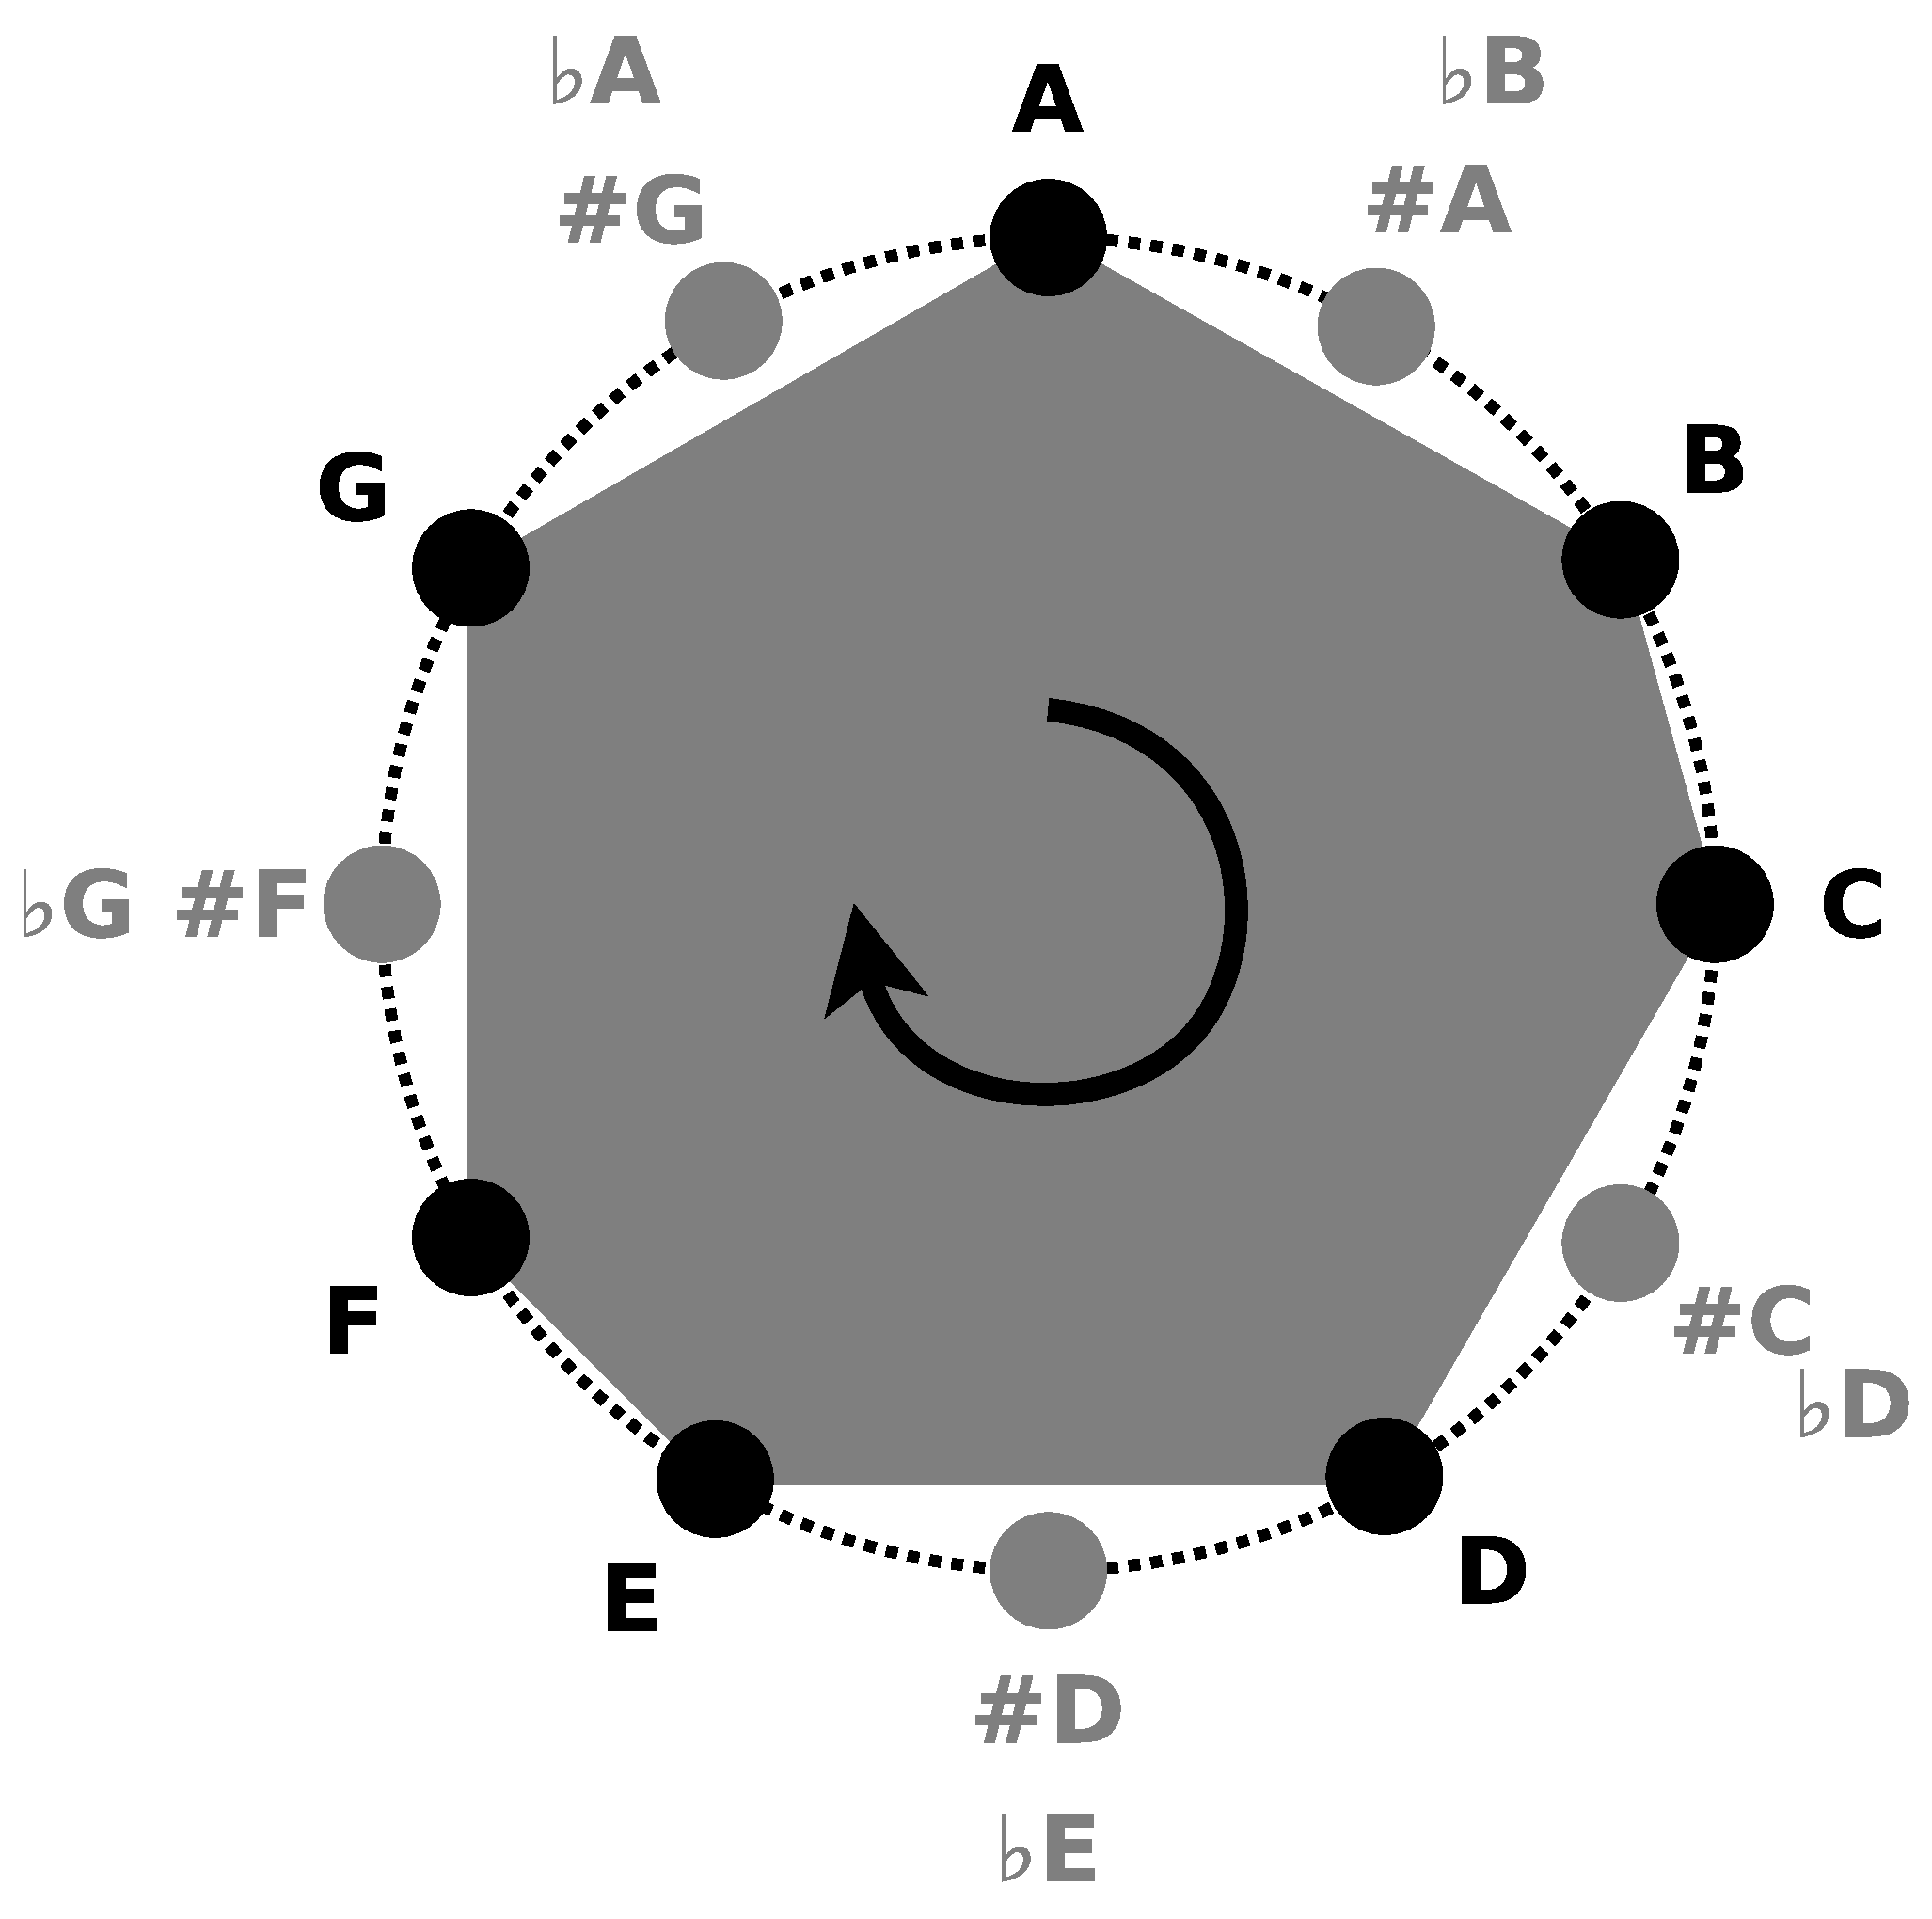
\includegraphics[width=0.65\textwidth]{chapters/cap-musica-basica/circulonotas.eps}
        \caption{Representação cíclica das distancias das notas musicais.}
        \label{fig:circulonotas}
    \end{figure}

Adicionalmente, na Figura \ref{fig:circulonotas}, 
está representada a escala diatônica com uma figura geométrica de 6 lados, 
colorido em cinza; e a escala cromática está representada com um circulo de linha pontuada.


     
%%%%%%%%%%%%%%%%%%%%%%%%%%%%%%%%%%%%%%%%%%%%%%%%%%%%%%%%%%%%%%%%%%%%%%%%%%%%%%%%
\section{\textcolor{blue}{Tipos de pauta}}
\label{sec:tipospauta}

%%%%%%%%%%%%%%%%%%%%%%%%%%%%%%%%%%%%%%%%%%%%%%%%%%%%%%%%%%%%%%%%%%%%%%%%%%%%%%%%
%%%%%%%%%%%%%%%%%%%%%%%%%%%%%%%%%%%%%%%%%%%%%%%%%%%%%%%%%%%%%%%%%%%%%%%%%%%%%%%%
\subsection{Pauta ou Pentagrama}\index{Pauta}
\label{sec:pauta}
A pauta está representada por 5 linhas paralelas e horizontais, 
as figuras musicais podem ocupar as linhas ou um lugar médio, entre elas.
Adicionalmente, lugares fora da pauta podem ser usados; 
para este proposito, linhas adicionais e parcialmente desenhadas, serão colocadas \cite[pp. 10]{cardoso1973curso}
como é mostrado na Figura \ref{fig:abc-pauta5}.
\begin{figure}[H]
\centering
\begin{abc}[name=abc-pauta5]
% abcm2ps pauta5.abc  -O pauta5.ps
% ps2epsi pauta5.ps pauta5.eps
%
X: 1 % start of header
K: none stafflines=5 %K: C %% Escala de C mayor %
M: none % M: 2/4
%T: Contratempo num compasso binário
V:1 clef=none stem=up name="Pauta"   sname="Pauta"
%
[V:1] C8 D8 E8 F8 G8 A8 B8 C'8 D'8 E'8 F'8 G'8 A'8
\end{abc}
\caption{Pauta com 5 linhas e figuras musicais mostrando algumas posições usáveis.}
\label{fig:abc-pauta5}
\end{figure}
A ordem de leitura das figuras musicais na pauta é de esquerda a direita,
e indica o avanço  do tempo;
as posições das linhas indicam um ordem crescente na altura do som que representam as figuras,
contando desde a linha inferior ate a superior. Nesse sentido, 
uma pauta é semelhante a um espectrograma, onde o eixo X representa o tempo,
o eixo Y representa a frequência, e a figuras colocadas em distintas posições do plano XY, descrevem
o comportamento do sonido nesses dois âmbitos. Assim, a Figura \ref{fig:abc-pauta5}
representa um conjunto de 13 sonidos, cada um com a mesma duração; 
porem, executado com diferentes alturas e em ordem crescente, 
desde um sonido grave ate um sonido mais agudo.
\begin{remark}
As linhas da pauta se contam de abaixo para acima.
As figuras musicais, se leem de esquerda direita, para que corresponda com o sentido do avanço do tempo.
\end{remark}


Por outro lado, se as figuras musicais podem ocupar varias posições entre as linhas da pauta,
pois estos lugares representam alturas diferentes do som; então, 
os silêncios não precisam desta característica,
pelo qual os símbolos que representam os silêncios tem uma posição fixa na pauta,
como pode ser visto na Figura \ref{fig:abc-pautasilencio}.
\begin{figure}[h]
\centering
\begin{abc}[name=abc-pautasilencio]
% abcm2ps pautasilencio.abc  -O pautasilencio.ps
% ps2epsi pautasilencio.ps pautasilencio.eps
%
X: 1 % start of header
K: none stafflines=5 %K: C %% Escala de C mayor %
M: none % M: 2/4
%T: Contratempo num compasso binário
V:1 clef=none name="Pauta"   sname="Pauta"
%
[V:1] z8 z4 z2 z1 z/2 z/4 G8 A4 B2 C'1 D'/2 E'/4 
\end{abc}
\caption{Pauta com 5 linhas e silêncios musicais mostrando algumas posições usáveis.}
\label{fig:abc-pautasilencio}
\end{figure}

O ponto mais interessante, é ver a diferencia do uso  da pausa de mínima e da pausa de semibreve,
dado que estes dois tipos de pausa usam o mesmo símbolo, porem em distintas posições.
Na Figura \ref{fig:abc-pautasilencio} a pausa de semibreve, 
está colocada em primeiro lugar desde a esquerda da pauta,
e o símbolo está desenhado unido a parte baixa de uma linha da pauta.
Por outro lado, a pausa de mínima está desenhada no segundo lugar da pauta,
contando desde a esquerda, e se desenha unida à parte de acima de uma linha da pauta.
Estos dois simbolo podem estar desenhados em duas linhas diferentes, 
como no exemplo da Figura \ref{fig:abc-pautasilencio}, ou na mesma linha.

\subsubsection{As claves na pauta}
\label{subsubsec:clavespauta}
A clave, como símbolo, 
se coloca ao inicio da pauta, 
e serve para indicar as alturas das notas na pauta \cite[pp. 179]{apel1969harvard} \cite[pp. 10]{cardoso1973curso}.
Existem 3 tipos de claves\footnote{E varias posições para estas, porem aqui veremos as mas basicas.} que podem ser usadas na pauta, 
assim temos: 
\begin{description}
\item [Clave sol:] Representada pelo símbolo 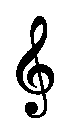
\includegraphics[height=14pt]{chapters/cap-musica-basica/G-clef.eps}. 
A posição donde esta clave se assine indica o lugar onde se localiza uma nota sol.
\begin{example}
Na Figura \ref{fig:abc-clavesol} podemos ver à clave de sol assinada sobre a segunda linha da pauta,
indicando que esta linha representa a nota sol.
\end{example} 
\item [Clave de fá:] Representada pelo símbolo 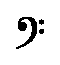
\includegraphics[height=10pt]{chapters/cap-musica-basica/FClef.eps}. 
A posição donde essa clave se assine indica o lugar onde se localiza uma nota fá.
\begin{example}
Na Figura \ref{fig:abc-clavefa} podemos ver à clave de fá assinada sobre a quarta linha da pauta,
indicando que essa linha representa a nota fá.
\end{example} 
\item [Clave de dó:] Representada pelo símbolo 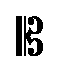
\includegraphics[height=10pt]{chapters/cap-musica-basica/CClef.eps}.
A posição donde esta clave se assine indica o lugar onde se localiza uma nota dó.
\begin{example}
Na Figura \ref{fig:abc-clavedo} podemos ver à clave de dó assinada sobre a terceira linha da pauta,
indicando que essa linha representa a nota dó.
\end{example} 
\end{description}
%%%
\begin{figure}[h]
    \centering
\begin{subfigure}[c]{0.25\textwidth}
\begin{abc}[name=abc-clavesol]
% abcm2ps clavesol.abc  -O clavesol.ps
% ps2epsi clavesol.ps clavesol.eps
%
X: 1 % start of header
K: C stafflines=5 %K: C %% Escala de C mayor %
M: none % M: 2/4
%T: Contratempo num compasso binário
V:1 clef=treble %name="Pauta com clave de sol"   sname="Pauta com clave de sol"
%
[V:1] G8
\end{abc}
\caption{Clave de sol com uma semibreve colocada em sol.}
\label{fig:abc-clavesol}
\end{subfigure}
~ %
\begin{subfigure}[c]{0.25\textwidth}
\begin{abc}[name=abc-clavefa]
% abcm2ps clavesfa.abc  -O clavefa.ps
% ps2epsi clavefa.ps clavefa.eps
%
X: 1 % start of header
K: C stafflines=5 %K: C %% Escala de C mayor %
M: none % M: 2/4
%T: Contratempo num compasso binário
V:1 clef=bass %name="Pauta com clave de fá"   sname="Pauta com clave de fá"
%
[V:1] F,8  
\end{abc}
\caption{Clave de fá com uma semibreve colocada em fá.}
\label{fig:abc-clavefa}
\end{subfigure}
~ %
\begin{subfigure}[c]{0.25\textwidth}
\begin{abc}[name=abc-clavedo]
% abcm2ps clavesfa.abc  -O clavedo.ps
% ps2epsi clavedo.ps clavedo.eps
%
X: 1 % start of header
K: C stafflines=5 %K: C %% Escala de C mayor %
M: none % M: 2/4
%T: Contratempo num compasso binário
V:1 clef=C %name="Pauta com clave de fá"   sname="Pauta com clave de fá"
%
[V:1] C8 
\end{abc}
\caption{Clave de dó com uma semibreve colocada em dó.}
\label{fig:abc-clavedo}
\end{subfigure}
    \caption{Tipos de claves}\label{fig:allclaves}
\end{figure}



\subsubsection{As claves e a escala diatonica}
Conhecida as definições das claves, e da \hyperref[sec:pos:Diatonica]{\textbf{escala diatônica}}, 
podemos misturar estes dois conceitos para conhecer a posição de todas as notas na pauta
\cite[pp. 10]{cardoso1973curso} \cite[pp. 14]{medteoria}.

Por exemplo, as pautas desenhadas na Figura \ref{fig:allnotesclaves} 
contem duas duas oitavas cada uma, centradas em dó, e com notas escritas usando semibreves.
\begin{figure}[h]
    \centering
\begin{abc}[name=abc-clavenotessol]
% abcm2ps clavenotessol.abc  -O clavenotessol.ps
% ps2epsi clavenotessol.ps clavenotessol.eps
%
X: 1 % start of header
K: C stafflines=5 %K: C %% Escala de C mayor %
M: none % M: 2/4
%T: Contratempo num compasso binário
V:1 clef=treble %name="Pauta com clave de sol"   sname="Pauta com clave de sol"
%
[V:1] "dó"C,8 "ré"D,8 "mi"E,8 "fá"F,8  "sol"G,8 "lá"A,8 "si"B,8 "dó"C8 "ré"D8 "mi"E8 "fá"F8  "sol"G8 "lá"A8 "si"B8 "dó"C'8 
\end{abc}

\begin{abc}[name=abc-clavenotesfa]
% abcm2ps clavenotesfa.abc  -O clavenotesfa.ps
% ps2epsi clavenotesfa.ps clavenotesfa.eps
%
X: 1 % start of header
K: C stafflines=5 %K: C %% Escala de C mayor %
M: none % M: 2/4
%T: Contratempo num compasso binário
V:1 clef=bass %name="Pauta com clave de fá"   sname="Pauta com clave de fá"
%
[V:1] C,8 D,8 E,8 F,8 G,8 A,8 B,8 C8 D8 E8 F8 G8 A8 B8 C'8 
\end{abc}

\begin{abc}[name=abc-clavenotesdo]
% abcm2ps clavenotesfa.abc  -O clavenotesdo.ps
% ps2epsi clavenotesdo.ps clavenotesdo.eps
%
X: 1 % start of header
K: C stafflines=5 %K: C %% Escala de C mayor %
M: none % M: 2/4
%T: Contratempo num compasso binário
V:1 clef=C %name="Pauta com clave de fá"   sname="Pauta com clave de fá"
%
[V:1] C,8 D,8 E,8 F,8 G,8 A,8 B,8 C8 D8 E8 F8 G8 A8 B8 C'8 
\end{abc}
    \caption{Tipos de claves}\label{fig:allnotesclaves}
\end{figure}
Na pauta com clave de sol, 
se distingue como as notas da oitava mais alta estão bem posicionadas na pauta;
porem, as notas da oitava inferior precisam linhas adicionais para serem representadas,
o que dificultará ou não deixará muito elegante a leitura dos elementos na pauta.
Podemos ver um caso similar, pero ao contrario, com a pauta que usa uma clave de fá;
nela, as notas da primeira oitava estão comodamente representadas dentro da pauta;
porem, as da oitava superior precisam linhas adicionais.
Finalmente, a notas escritas usando a clave de dó, estão bem centradas,
para notas com alturas intermédias e só fica fora da pauta as duas notas mais aguda e as duas mais graves.

A primeira vista poderia parecer mais vantajosa a clave de do, 
porem isto acontece só porque a nota central que queremos representar é um dó,
teríamos uma vantagem similar na clave de sol, se usaremos uma nota central em si,
ou a vantagem a teríamos na clave de fá, se usaremos uma nota central em ré. 
Na prática, escolher entre
uma clave u outra dependerá da melodia que queiramos encaixar na pauta.
Porem existe uma combinação muito usada na musica para piano, 
que é usar uma clave de sol pra descrever as melodias a serem tocadas pela mão direita,
e usar uma clave de fá, para as que serão tocadas pela mão esquerda; 
isto é conveniente devido a que se olhamos o dó central nessas claves, 
na Figura \ref{fig:allnotesclaves}, 
poderemos observar que esta nota se sai das linhas da pauta, 
justo para entrar nas linhas da pauta da outra mão.

%%%%%%%%%%%%%%%%%%%%%%%%%%%%%%%%%%%%%%%%%%%%%%%%%%%%%%%%%%%%%%%%%%%%%%%%%%%%%%%%
%%%%%%%%%%%%%%%%%%%%%%%%%%%%%%%%%%%%%%%%%%%%%%%%%%%%%%%%%%%%%%%%%%%%%%%%%%%%%%%%
\subsection{\textcolor{green}{Pauta de percussão}}\index{Pauta!Pauta de Percussão}

Existem varias formas de representar as pautas para percussão, 
estas são diferenciadas do pentagrama, devido a que na percussão, 
na maioria dos casos não se tem controle da \hyperref[sec:pos:Duracion]{\textbf{duração}} do som;
e sim se tem, do momento em que este será executado. Em outros casos,
pode estar desabilitada a possibilidade de mudar a \hyperref[sec:pos:Altura]{\textbf{altura}} dos sons;
pelo que não se necessitam linhas pra representar estas alturas.
Assim, as pautas de percussão estarão optimizadas, em cada caso, 
para mostrar com simplicidade o ritmo que se deseja interpretar.

\subsubsection{A clave de percussão}
Também chamada \textbf{clave neutral} ou \textbf{clave de ritmos}, 
porque é usada por percussionistas, bateristas, 
ou usada para qualquer instrumento que produz um som que não tem uma altura definida \cite[pp. 51]{harnum2009basic}.
Asim, esta clave indica que a pauta mostra ritmos e modos de tocar um instrumento, 
e não indica as alturas das notas, 
como outras claves mostradas na Seção \ref{subsubsec:clavespauta}.
Podemos achar dois símbolos equivalentes para representar esta clave, 
estes são \includegraphics[height=10pt]{chapters/cap-musica-basica/P1-clef.eps}
e \includegraphics[height=10pt]{chapters/cap-musica-basica/P2-clef.eps}.
Entre os instrumentos que usam esta clave temos:
o tambourine, o triangulo, o pandeiro, etc.
A Figura \ref{fig:allpercusionclaves} mostra algumas formas de usar a clave de percussão,
sendo formas equivalentes, as mostradas na Figura \ref{fig:abc-claveperczero} e a Figura \ref{fig:abc-clavepercuma}.

\begin{figure}[h]
    \centering 
\begin{subfigure}[c]{0.24\textwidth}
\begin{abc}[name=abc-clavepercusion1]
% abcm2ps clavepercusion1.abc  -O clavepercusion1.ps
% ps2epsi clavepercusion1.ps clavepercusion1.eps
%
X: 1 % start of header
K: C stafflines=0 %K: C %% Escala de C mayor %
M: none % M: 2/4
%T: Contratempo num compasso binário
V:1 clef=perc stem=up %name="Pauta com clave de fá"   sname="Pauta com clave de fá"
%
[V:1] B1 B1 B2 B1 B2   
\end{abc}
\caption{Clave de percussão sem linhas, indicando que só existe um modo de tocar o instrumento.}
\label{fig:abc-claveperczero}
\end{subfigure}
~%
\begin{subfigure}[c]{0.24\textwidth}
\begin{abc}[name=abc-clavepercusion2a]
% abcm2ps clavepercusion2a.abc  -O clavepercusion2a.ps
% ps2epsi clavepercusion2a.ps clavepercusion2a.eps
%
X: 1 % start of header
K: C stafflines=1 %K: C %% Escala de C mayor %
M: none % M: 2/4
%T: Contratempo num compasso binário
V:1 clef=perc stem=up %name="Pauta com clave de fá"   sname="Pauta com clave de fá"
%
[V:1] B1 B1 B2 B1 B2   
\end{abc}
\caption{Clave de percussão com uma linha e só um modo de tocar o instrumento.}
\label{fig:abc-clavepercuma}
\end{subfigure}
~%
\begin{subfigure}[c]{0.24\textwidth}
\begin{abc}[name=abc-clavepercusion2]
% abcm2ps clavepercusion2.abc  -O clavepercusion2.ps
% ps2epsi clavepercusion2.ps clavepercusion2.eps
%
X: 1 % start of header
K: C stafflines=1 %K: C %% Escala de C mayor %
M: none % M: 2/4
%T: Contratempo num compasso binário
V:1 clef=perc stem=up %name="Pauta com clave de fá"   sname="Pauta com clave de fá"
%
[V:1] A1 C'1 A2 C'1 A2   
\end{abc}
\caption{Clave de percussão com uma linha e dois modos de tocar o instrumento.}
\label{fig:abc-clavepercum2}
\end{subfigure}
~%
\begin{subfigure}[c]{0.24\textwidth}
\begin{abc}[name=abc-clavepercusion3]
% abcm2ps clavepercusion3.abc  -O clavepercusion3.ps
% ps2epsi clavepercusion3.ps clavepercusion3.eps
%
X: 1 % start of header
K: C stafflines=5 %K: C %% Escala de C mayor %
M: none % M: 2/4
%T: Contratempo num compasso binário
V:1 clef=perc stem=up %name="Pauta com clave de fá"   sname="Pauta com clave de fá"
%
[V:1] A1 B1 G2 C'1 F2   
\end{abc}
\caption{Clave de percussão com cinco linhas e vários modos de tocar o instrumento.}
\label{fig:abc-claveperccinco}
\end{subfigure}
    \caption{Usos da clave de percussão}\label{fig:allpercusionclaves}
\end{figure}

\subsubsection{O sistema de notação monolinear}
Este sistema foi criado pelo baterista suiço, Dr. Fritz Berger, em 1928. 
Ele o chamou ``the monolinear notation system'', 
de modo que seu sistema utilizava uma única linha na pauta, na sua definição,
a parte de acima da linha representava a mão direita (para bateria), e
a parte de abaixo da linha a mão esquerda.
Assim, era mais fácil ler os ritmos, deixando claro que mão devia fazer uma determinada ação
\cite[pp. 148]{beck1995encyclopedia} \cite[pp. 332]{dean2012drum}.
Um exemplo deste sistema pode ser visto na Figura \ref{fig:abc-clavepercum2}.

\subsubsection{The grid notation}


\cite[pp. 289]{gould676behind}

\begin{comment}
\subsubsection{The musical notation of percusion}
Revisar  \cite[pp. 70]{harnum2009basic}

Figura \ref{fig:abc-musicalperc}
\begin{figure}[H]
\centering
\begin{abc}[name=abc-musicalperc]
% abcm2ps musicalperc.abc  -O musicalperc.ps
% ps2epsi musicalperc.ps musicalperc.eps
%
X:1
T:Drum Key
M:
L:1/4
K:C clef=perc
"^Bass"F|"^Snare"c|"^High tom"e|"^Mid tom"d|"^Low tom"B|"^Floor tom"A|
"^Cymbal"^b|"^Crash"^a|"^Hi-hat"^g|"^Ride"^f|"^Hi-hat Pedal"^D|]

\end{abc}
\caption{Figuras e pausas}
\label{fig:abc-musicalperc}
\end{figure}
\end{comment}



%%%%%%%%%%%%%%%%%%%%%%%%%%%%%%%%%%%%%%%%%%%%%%%%%%%%%%%%%%%%%%%%%%%%%%%%%%%%%%%%

%%%%%%%%%%%%%%%%%%%%%%%%%%%%%%%%%%%%%%%%%%%%%%%%%%%%%%%%%%%%%%%%%%%%%%%%%%
\section{Intervalo melódico}
\label{sec:intervalomelodico}
\index{Música!Intervalo}
\index{Música!Intervalo melódico}


Um intervalo é a distância que existe entre dois sons de alturas definidas;
os intervalos melódicos correspondem à medição de notas musicais executadas uma após outra, 
numa melodia \cite[pp. 17]{holst1998abc}.
Assim, podem existir intervalos melódicos ascendentes ou descendentes,
que indicam que o tom da nota posterior é mais agudo ou mais grave, respetivamente \cite[pp. 17]{holst1998abc}.

Sobre a unidade de medição que será usada para quantificar as distancias nos intervalos, 
estes podem ser medidos usando sua posição relativa seguindo as sete notas da escala diatônica \cite[pp. 17]{holst1998abc}.
Por exemplo na Tabela \ref{tab:intervalomelodico} podemos ver os nomes usados seguindo esta notação.  
\begin{table}[h]
  \centering
  \begin{tabular}{|l|l||l|l|}
  \hline
  Intervalo & Posição     & Intervalo & Posição \\ \hline \hline
  Uníssono  & 1$^{\circ}$ & Segunda   & 2$^{\circ}$ \\ \hline
  Terça     & 3$^{\circ}$ & Quarta    & 4$^{\circ}$ \\ \hline
  Quinta    & 5$^{\circ}$ & Sexta     & 6$^{\circ}$ \\ \hline
  Sétima    & 7$^{\circ}$ & Oitava    & 8$^{\circ}$ \\ \hline
  \end{tabular}
  \caption{Distancia entre intervalos.}
  \label{tab:intervalomelodico}
\end{table}

Na Figura \ref{fig:abc-isegunda1} podemos ver um intervalo de uma segunda ascendente,
desde um dó ate um ré (+2 semitons).
Na Figura \ref{fig:abc-isegunda2} podemos ver um intervalo de uma segunda descendente,
desde um fá ate um mi (-1 semitons).
\begin{figure}[H]
    \centering
    \begin{subfigure}[b]{0.4\textwidth}
\begin{abc}[name=abc-isegunda1]
X: 1 % start of header
K: C % scale: C major
V:1 %name="Pauta com clave de fá"   sname="Pauta com clave de fá"
[V:1]  C2 D2
w: ~1º ~2º
\end{abc}
\caption{Intervalo de uma segunda ascendente.}
\label{fig:abc-isegunda1}
    \end{subfigure}
    \quad%~%add desired spacing between images, e. g. ~, \quad, \qquad, \hfill etc. 
      %(or a blank line to force the subfigure onto a new line)
    \begin{subfigure}[b]{0.4\textwidth}
\begin{abc}[name=abc-isegunda2]
X: 1 % start of header
K: C % scale: C major
V:1 %name="Pauta com clave de fá"   sname="Pauta com clave de fá"
[V:1]  F2 E2
w: ~1º ~2º
\end{abc}
\caption{Intervalo de uma segunda descendente.}
\label{fig:abc-isegunda2}
    \end{subfigure}
    \caption{Intervalo melódico de uma segunda.}
    \label{fig:intervalosegunda}
\end{figure}


Na Figura \ref{fig:abc-iterca1} podemos ver um intervalo de uma terça ascendente,
desde um fá ate um lá (+4 semitons).
Na Figura \ref{fig:abc-iterca2} podemos ver um intervalo de uma terça descendente,
desde um dó ate um lá (-3 semitons) \cite[pp. 16-17]{holst1998abc}.
\begin{figure}[H]
    \centering
    \begin{subfigure}[b]{0.4\textwidth}
\begin{abc}[name=abc-iterca1]
X: 1 % start of header
K: C % scale: C major
V:1 %name="Pauta com clave de fá"   sname="Pauta com clave de fá"
[V:1]  F2 A2
w: ~1º ~3º
\end{abc}
\caption{Intervalo de uma terça ascendente.}
\label{fig:abc-iterca1}
    \end{subfigure}
    \quad%~%add desired spacing between images, e. g. ~, \quad, \qquad, \hfill etc. 
      %(or a blank line to force the subfigure onto a new line)
    \begin{subfigure}[b]{0.4\textwidth}
\begin{abc}[name=abc-iterca2]
X: 1 % start of header
K: C % scale: C major
V:1 %name="Pauta com clave de fá"   sname="Pauta com clave de fá"
[V:1]  |C'2 A2|
w: ~1º ~3º
\end{abc}
\caption{Intervalo de uma terça descendente.}
\label{fig:abc-iterca2}
    \end{subfigure}
    \caption{Intervalo melódico de uma terça.}
    \label{fig:intervaloterca}
\end{figure}



Na Figura \ref{fig:abc-iquarta1} podemos ver um intervalo de uma quarta ascendente,
desde um sol ate um dó (+5 semitons) \cite[pp. 17]{holst1998abc}.
Na Figura \ref{fig:abc-iquarta2} podemos ver um intervalo de uma quarta descendente,
desde um sol ate um ré (-5 semitons).
\begin{figure}[H]
    \centering
    \begin{subfigure}[b]{0.4\textwidth}
\begin{abc}[name=abc-iquarta1]
X: 1 % start of header
K: C % scale: C major
V:1 %name="Pauta com clave de fá"   sname="Pauta com clave de fá"
[V:1]  G2 C'2
w: ~1º ~4º
\end{abc}
\caption{Intervalo de uma quarta ascendente.}
\label{fig:abc-iquarta1}
    \end{subfigure}
    \quad%~%add desired spacing between images, e. g. ~, \quad, \qquad, \hfill etc. 
      %(or a blank line to force the subfigure onto a new line)
    \begin{subfigure}[b]{0.4\textwidth}
\begin{abc}[name=abc-iquarta2]
X: 1 % start of header
K: C % scale: C major
V:1 %name="Pauta com clave de fá"   sname="Pauta com clave de fá"
[V:1]  G2 D2
w: ~1º ~4º
\end{abc}
\caption{Intervalo de uma quarta descendente.}
\label{fig:abc-iquarta2}
    \end{subfigure}
    \caption{Intervalo melódico de uma quarta.}
    \label{fig:intervaloquarta}
\end{figure}

Na Figura \ref{fig:abc-iquinta1} podemos ver um intervalo de uma quinta ascendente,
desde um si ate um fá (+6 semitons).
Na Figura \ref{fig:abc-iquinta2} podemos ver um intervalo de uma quinta descendente,
desde um dó ate um fá (-7 semitons) \cite[pp. 17]{holst1998abc}.
\begin{figure}[H]
    \centering
    \begin{subfigure}[b]{0.4\textwidth}
\begin{abc}[name=abc-iquinta1]
X: 1 % start of header
K: C % scale: C major
V:1 %name="Pauta com clave de fá"   sname="Pauta com clave de fá"
[V:1]  B,2 F2
w: ~1º ~5º
\end{abc}
\caption{Intervalo de uma quinta ascendente.}
\label{fig:abc-iquinta1}
    \end{subfigure}
    \quad%~%add desired spacing between images, e. g. ~, \quad, \qquad, \hfill etc. 
      %(or a blank line to force the subfigure onto a new line)
    \begin{subfigure}[b]{0.4\textwidth}
\begin{abc}[name=abc-iquinta2]
X: 1 % start of header
K: C % scale: C major
V:1 %name="Pauta com clave de fá"   sname="Pauta com clave de fá"
[V:1]  C'2 F2
w: ~1º ~5º
\end{abc}
\caption{Intervalo de uma quinta descendente.}
\label{fig:abc-iquinta2}
    \end{subfigure}
    \caption{Intervalo melódico de uma quinta.}
    \label{fig:intervaloquinta}
\end{figure}

Na Figura \ref{fig:abc-isexta1} podemos ver um intervalo de uma sexta ascendente,
desde um dó ate um lá (+9 semitons).
Na Figura \ref{fig:abc-isexta2} podemos ver um intervalo de uma sexta descendente,
desde um mi ate um sol (-9 semitons) \cite[pp. 18]{holst1998abc}.
\begin{figure}[H]
    \centering
    \begin{subfigure}[b]{0.4\textwidth}
\begin{abc}[name=abc-isexta1]
X: 1 % start of header
K: C % scale: C major
V:1 %name="Pauta com clave de fá"   sname="Pauta com clave de fá"
[V:1]  C2 A2
w: ~1º ~6º
\end{abc}
\caption{Intervalo de uma sexta ascendente.}
\label{fig:abc-isexta1}
    \end{subfigure}
    \quad%~%add desired spacing between images, e. g. ~, \quad, \qquad, \hfill etc. 
      %(or a blank line to force the subfigure onto a new line)
    \begin{subfigure}[b]{0.4\textwidth}
\begin{abc}[name=abc-isexta2]
X: 1 % start of header
K: C % scale: C major
V:1 %name="Pauta com clave de fá"   sname="Pauta com clave de fá"
[V:1]  E'2 G2
w: ~1º ~6º
\end{abc}
\caption{Intervalo de uma sexta descendente.}
\label{fig:abc-isexta2}
    \end{subfigure}
    \caption{Intervalo melódico de uma sexta.}
    \label{fig:intervalosexta}
\end{figure}

Na Figura \ref{fig:abc-isetima1} podemos ver um intervalo de uma sétima ascendente,
desde um ré ate um dó (+10 semitons) \cite[pp. 18]{holst1998abc}.
Na Figura \ref{fig:abc-isetima2} podemos ver um intervalo de uma sétima descendente,
desde um si ate um dó (-11 semitons).
\begin{figure}[H]
    \centering
    \begin{subfigure}[b]{0.4\textwidth}
\begin{abc}[name=abc-isetima1]
X: 1 % start of header
K: C % scale: C major
V:1 %name="Pauta com clave de fá"   sname="Pauta com clave de fá"
[V:1]  D2 C'2
w: ~1º ~7º
\end{abc}
\caption{Intervalo de uma sétima ascendente.}
\label{fig:abc-isetima1}
    \end{subfigure}
    \quad%~%add desired spacing between images, e. g. ~, \quad, \qquad, \hfill etc. 
      %(or a blank line to force the subfigure onto a new line)
    \begin{subfigure}[b]{0.4\textwidth}
\begin{abc}[name=abc-isetima2]
X: 1 % start of header
K: C % scale: C major
V:1 %name="Pauta com clave de fá"   sname="Pauta com clave de fá"
[V:1]  E'2 G2
w: ~1º ~7º
\end{abc}
\caption{Intervalo de uma sétima descendente.}
\label{fig:abc-isetima2}
    \end{subfigure}
    \caption{Intervalo melódico de uma sétima.}
    \label{fig:intervalosetima}
\end{figure}

%%%%%%%%%%%%%%%%%%%%%%%%%%%%%%%%%%%%%%%%%%%%%%%%%%%%%%%%%%%%%%%%%%%%%%%%%%%%%%%%
\subsection{Qualidade do intervalo}
Além do uso de notas musicais para quantificar o intervalo, 
estos também podem ter uma qualificação,
os intervalos de 4$^{\circ}$, 5$^{\circ}$ e 8$^{\circ}$ são chamados justos,
e os intervalos 2$^{\circ}$, 3$^{\circ}$, 6$^{\circ}$  e 7$^{\circ}$ são chamados maiores \cite[pp. 19]{bennett1993elementos}.

A Figura \ref{fig:justo-maior} mostra as possibilidades que podem tomar as qualificações.
\begin{figure}[h]
  \centering
    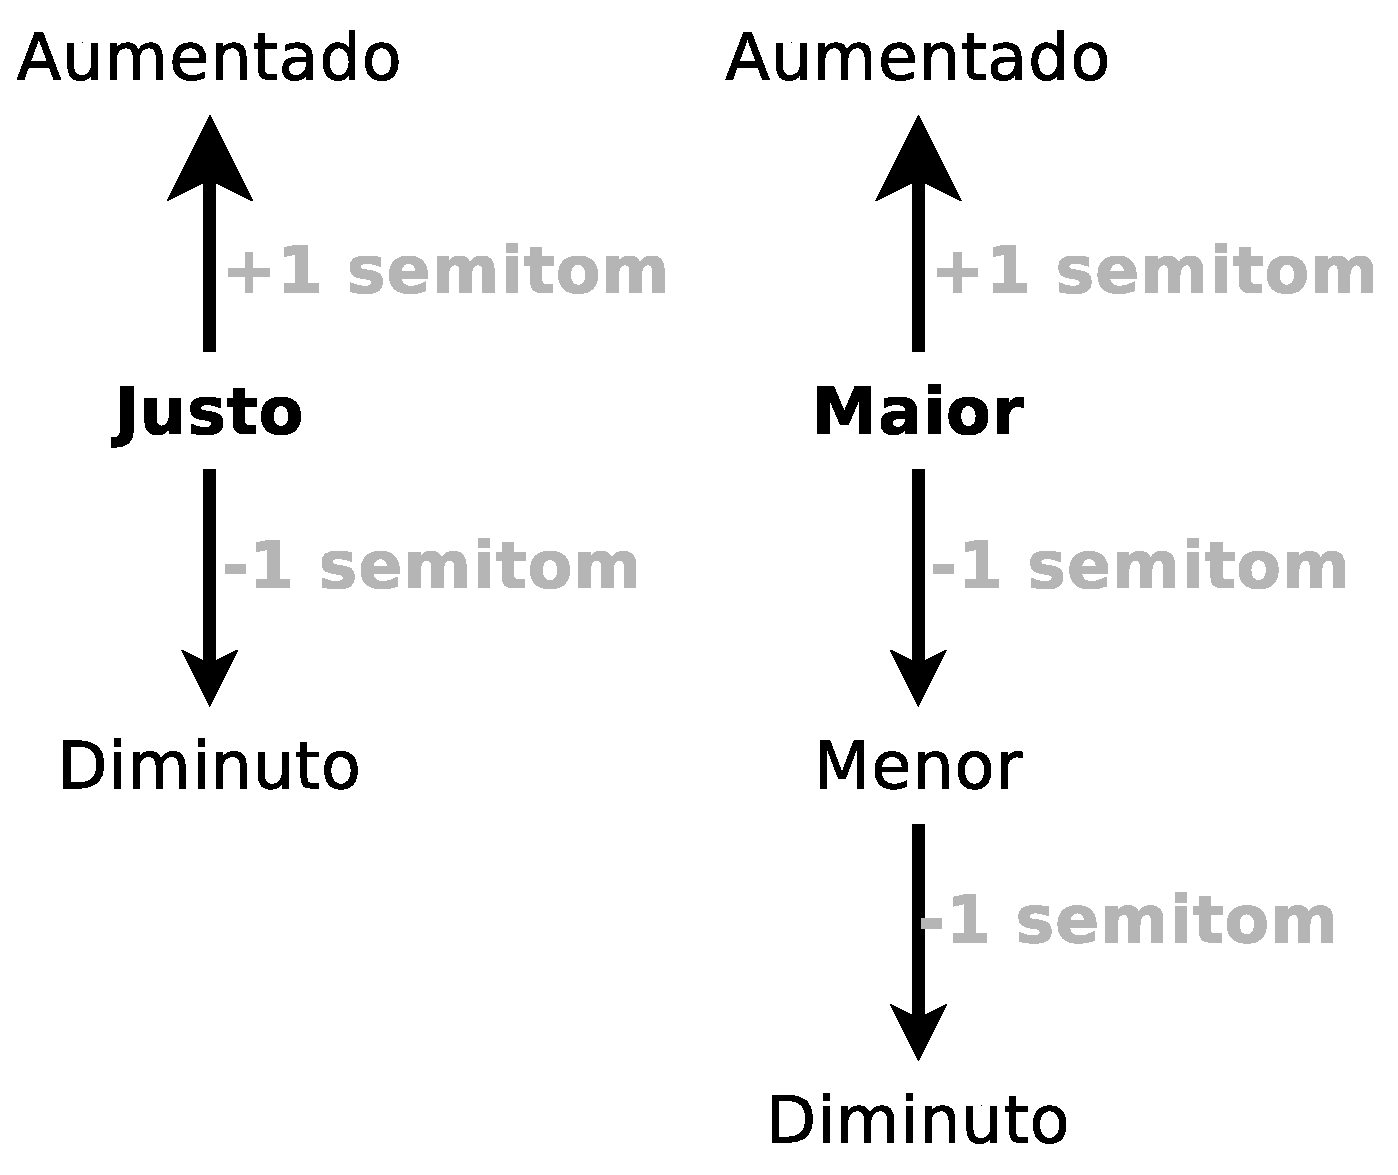
\includegraphics[width=0.5\textwidth]{chapters/cap-musica-basica/justo-maior.eps}
  \caption{Intervalos justos maiores e menores.}
  \label{fig:justo-maior}
\end{figure}
Uma forma rápida de lembrar os nomes é seguindo a escala em dó maior, como 
na Figura \ref{fig:abc-justo-maior2}, onde M indica maior e J indica justo. 
\begin{figure}[H]
    \centering
\begin{abc}[name=abc-justo-maior2]
X: 1 % start of header
K: C % scale: C major
V:1 %name="Pauta com clave de fá"   sname="Pauta com clave de fá"
[V:1]  C8 D8 E8 F8 G8 A8 B8 C'8
w:     ~1ºJ ~2ºM ~3ºM ~4ºJ ~5ºJ ~6ºM ~7ºM ~8ºJ
\end{abc}
\caption{Intervalo de uma sétima descendente.}
\label{fig:abc-justo-maior2}
\end{figure}



A Tabela \ref{tab:intervalomelodico2} mostra o número de semitons 
correspondente a cada intervalo \cite[pp. 89-90]{cardoso1973curso} \cite[pp. 72-74]{holst1998abc}.

\begin{table}[h]
  \centering
  \begin{tabular}{|l|l|l|l|}
  \hline
  \textbf{Intervalo} & \textbf{Semitons} & \textbf{Tons} & \textbf{Exemplo}     \\ \hline \hline
  ~                & 0        & 0        & dó \\ \hline
  Segunda menor    & 1        & 1/2      & ré$\flat$ \\ \hline
  Segunda maior    & 2        & 1        & ré        \\ \hline  \hline
  Terça menor      & 3        & 1+1/2    & mi$\flat$ \\ \hline
  Terça maior      & 4        & 2        & mi        \\ \hline  \hline
  \textbf{Quarta justa}     & \textbf{5}        & \textbf{2+1/2}    & \textbf{fá}        \\ \hline
  Quarta aumentada & 6        & 3        & fá$\#$    \\ \hline \hline
  Quinta diminuta  & 6        & 3        & sol$\flat$ \\ \hline 
  \textbf{Quinta justa}     & \textbf{7}        & \textbf{3+1/2}    & \textbf{sol}      \\ \hline \hline
  Sexta menor      & 8        & 4        & lá$\flat$ \\ \hline
  Sexta maior      & 9        & 4+1/2    & lá        \\ \hline \hline
  Sétima menor     & 10       & 5        & si$\flat$ \\ \hline
  Sétima maior     & 11       & 5+1/2    & si        \\ \hline \hline
  \textbf{Oitava justa}     & 12       & 6        & \textbf{dó} \\ \hline
  \end{tabular}
  \caption{Distancia entre intervalos.}
  \label{tab:intervalomelodico2}
\end{table}
         
%%%%%%%%%%%%%%%%%%%%%%%%%%%%%%%%%%%%%%%%%%%%%%%%%%%%%%%%%%%%%%%%%%%%%%%%%%%%%%%%
\section{\textcolor{green}{Compasso}}\index{Compasso}
\label{sec:compaso}

\begin{description}
\item[Compasso:] O dicionário de Harvard de música \cite[pp. 513]{apel1969harvard} define compasso (``measure'' em inglês)
como um grupo de tempos, batimentos ou pulsos (unidade do tempo musical),
onde o primeiro destes normalmente é acentuado. 
Este número de tempos no compasso pode ser, dois, trés, quatro, ou ocasionalmente 5 ou mais. 
Sendo estos compassos separados por barras verticais e as notas do compasso esquematizados baixo uma métrica.
\begin{example}
Figura \ref{fig:abc-exemplocompasso1}
\end{example}
 
\item[Métrica:] Sobre a métrica  (``meter'' em inglês) o dicionario \cite[pp. 523]{apel1969harvard} explica que é
um padrão de unidades temporais fixas, chamados batimentos, 
pelo qual um período de tempo de uma peça musical ou uma seção dela é medida. 
Agrega tambem que a métrica é indicado geralmente por uma fração, como por exemplo:
${2}/{2}$ , ${3}/{4}$ , ${4}/{4}$, etc. Em português esta fração é chamada de formula do compasso. 
\begin{example}
Figura \ref{fig:abc-exemplocompasso1}
\end{example}
\end{description}

O numerador, da formula do compasso, indica o número de pulsações (tempos) que compõem cada compasso.
Por outro lado o denominador nos informa al longitude temporal de cada um dos tempos do compasso.

\begin{figure}[h]
\centering
\begin{abc}[name=abc-exemplocompasso1]
% abcm2ps exemplocompasso1.abc  -O exemplocompasso1.ps
% ps2epsi exemplocompasso1.ps exemplocompasso1.eps
%
X: 1 % start of header
K: none stafflines=0 %K: C %% Escala de C mayor %
M: 2/4
%T: Contratempo num compasso binário
V:1 clef=perc stem=up name="Ritmo 1"   sname="Ritmo 1"
%
[V:1] | B2 B1 B1| B2 B1 B1 | B2 B1 B1 | B2 z2  |
%       
\end{abc}
\caption{Figuras e pausas}
\label{fig:abc-exemplocompasso1}
\end{figure}



A Tabela \ref{tab:abc-noteslength} exemplifica o significado do denominador da formula do compasso; 
\begin{table}[h]
\centering
\begin{tabular}{|c|c|c|c|}
\hline
denominador & Figura  & Duração & Nome\\ \hline
\hline
$1$   & \fullnote    & $S$   & Semibreve \\ \hline
$2$ & \halfnote    & $S/2$ & Mínima \\ \hline
$4$ & \quarternote & $S/4$ & Semínima \\ \hline
$8$ & \eighthnote  & $S/8$ & Colcheia \\ \hline
\end{tabular}
\caption{Duração e símbolos de algumas figuras musicais}
\label{tab:abc-noteslength}
\end{table}
onde a primeira coluna mostra o denominador da formula,
a segunda coluna mostra as figuras musicais que representam cada um dos tempos do compasso, e 
a terceira e quarta coluna, indicam a duração em segundos e o nome da figura musical.

podemos achar equivalências aos exemplos da formula do compasso dados
anteriormente; onde os compassos com formula $\mathbf{2}/2$ tem cada um, uma duração de $\mathbf{2}$\halfnote ~(duas mínimas),  
compassos com formula $\mathbf{3}/4$ tem uma duração de $\mathbf{3}$\quarternote ~(trés semínimas) 
e $\mathbf{4}/4$ uma duração de $\mathbf{4}$\quarternote ~(quatro semínimas). É importante
ressaltar que a duração em tempo das figuras musicais é relativa, como pode ser visto
na terceira coluna da Tabela \ref{tab:abc-noteslength}, onde as durações estão em função
da duração $S$ da semibreve. 


Se classificamos os compassos por sua métrica, os três tipos mais conhecidos 
são os compassos binários, ternários, quaternários \cite[pp. 27]{adolfo2002musica}.

\subsection{\textcolor{green}{Compasso binário}}\index{Compasso!Compasso Binário} Ou compasso binário simples,
é uma estrutura rítmica que se carateriza por ter compassos com uma  duração de dois tempos,
sendo o primeiro tempo forte (acentuado), e o segundo de tempo fraco (não acentuado)
\cite[pp. 41]{grabner2001teoria} \cite[pp. 66]{adolfo2002musica}\cite[pp. 28]{alves2004teoria}. 
Os compassos binários (simples) tem uma formula de compasso na forma $2/B$,
onde $B$ pode ser $2$, $4$, $8$, etc. 
A Figura \ref{compasso:binario}, representa um exemplo de compasso binário simples, 
com formula de compasso $2/2 \equiv 2$\halfnote, 
e tempos com uma duração de $S/2$ (uma \halfnote), 
sendo que o primeiro compasso contem $2$\halfnote~e o segundo contem $4$\quarternote.
Na Figura \ref{compasso:binario} a sigla ``N.A.'' significa ``Não acentuado'', pelo que é fácil perceber
que em qualquer caso, só a nota que é executada no tempo 1 é acentuada.
\begin{figure}[H]
\centering
\begin{abc}[name=abc-compasso1]
X: 1 % start of header
K: C % scale: C major
M: 2/2 %meter - compasso
"Primeiro compasso" G4 F4 |"Segundo compasso" G2 D2 F2 D2  |
w: Acentuado N.A. Acentuado N.A. N.A. N.A.
\end{abc}
\caption{Exemplo de compasso binário (simples)}
\label{compasso:binario}
\end{figure}

Se falamos de forma mais geral, 
podemos ter dois tipos de compassos binários: os simples e os compostos.
Assim, 
para achar a formula de um compasso composto, correspondente a um compasso simples (usando quialteras de três)
usamos a seguinte operação \cite[pp. 74]{alves2004teoria}, 
\begin{equation}\label{eq:comcomposto}
Compasso~simples\times\frac{3}{2}=Compasso~composto.
\end{equation}
De modo que obtemos compassos binários compostos com as seguintes formulas de compasso: 
$6/4$, $6/8$, $6/16$, etc.
A diferencia do visto nos compassos binários simples, os compassos binários compostos tem 
um pulso forte (Acentuado) no tempo 1 e um pulso semiforte (Acentuado porem menor) no tempo 4, 
de modo que os tempos 2,3,5 e 6,
são classificados como tempos fracos (Não Acentuados)\cite[pp. 41]{grabner2001teoria}.
A Figura \ref{compasso:binariocomposto}, representa um exemplo de compasso binário composto, 
com formula de compasso $6/4 \equiv 6$\quarternote, 
e tempos com uma duração de $S/4$ (uma \quarternote), 
sendo que o primeiro compasso contem $6$\quarternote~e o segundo contem dois $2$\quarternote~e dois $2$\halfnote.
Da Figura \ref{compasso:binariocomposto} é fácil perceber
que em qualquer caso, só são acentuados as nota que são executadas no tempo 1 e 4; 
aclarando que as notas executadas no tempo 4 tem uma acentuação menor que as executadas no tempo 1.
\begin{figure}[H]
\centering
\begin{abc}[name=abc-compasso1c]
X: 1 % start of header
K: C % scale: C major
M: 6/4 %meter - compasso
"Primeiro compasso" G2 D2 D2 F2 D2 D2 |"Segundo compasso" G2 D4 F2 D4  |
w: Acentuado N.A. N.A. Acentuado N.A N.A. Acentuado N.A. Acentuado N.A. 
\end{abc}
\caption{Exemplo de compasso binário composto}
\label{compasso:binariocomposto}
\end{figure}

Alguns autores consideram aos compassos quaternários (ex: 4/4, 4/8) como um caso de compasso binário,
chamando eles de compasso binário duplo \cite[pp. 41]{grabner2001teoria}.




\subsection{\textcolor{green}{Compasso ternário}}\index{Compasso!Compasso Ternário} Ou compasso ternário simples,
é uma estrutura rítmica que se carateriza por ter compassos com trés tempos,
sendo o primeiro pulso forte (acentuado) e os outros dois fracos (não acentuados) 
\cite[pp. 67]{adolfo2002musica}\cite[pp. 30]{alves2004teoria}. 
Os compassos ternários (simples) tem uma formula de compasso da forma $3/B$, 
onde $B$ pode ser $2$, $4$, $8$, etc.
Por exemplo temos, as formulas de compassos ternários simples: $3/2$, $3/4$, $3/8$,  etc.

A Figura \ref{compasso:ternario}, representa um exemplo de compasso ternário (simples), com 
formula de compasso $3/4 \equiv 3$\quarternote, 
onde os tempos tem uma duração de $S/4$, o primeiro compasso contem $3$\quarternote~e
o segundo contem $6$\eighthnote.
Na Figura \ref{compasso:ternario}  é fácil perceber
que em ambos compassos, só a nota que é executada no tempo 1 é acentuada.
\begin{figure}[H]
\centering
\begin{abc}[name=abc-compasso2]
X: 1 % start of header
K: C % scale: C major
M: 3/4 %meter - compasso
"Primeiro compasso" G2 F2 F2 |"Segundo compasso" G1 F1 E1 D1 D1  D1  |
w: Acentuado N.A. N.A. Acentuado N.A N.A.  N.A. N.A. N.A. 
\end{abc}
\caption{Exemplo de compasso ternário}
\label{compasso:ternario}
\end{figure}


São chamados de compassos ternários compostos,  
quando estes tem uma formula de compasso como: $9/4$, $9/8$ e $9/16$.
Para gerar estes compassos compostos a partir de suas versões simples,
se segue a mesma operação descrita na Equação \ref{eq:comcomposto}.


\subsection{\textcolor{green}{Compasso quaternário}}\index{Compasso!Compasso Quaternário} Ou compasso quaternário simples,
é uma estrutura rítmica que se carateriza por ter compassos com quatro tempos,
sendo o primeiro pulso forte (acentuado), o segundo fraco (não acentuado), 
o terceiro semiforte (acentuado porem menor) e o último fraco (não acentuado) 
\cite[pp. 67]{adolfo2002musica}\cite[pp. 32]{alves2004teoria}. 
Os compassos quaternários (simples) tem uma formula de compasso da forma $4/B$, 
onde $B$ pode ser $2$, $4$, $8$, etc.
Por exemplo temos, as formulas de compassos ternários simples: $4/2$, $4/4$, $4/8$,  etc.

A Figura \ref{compasso:quaternario}, representa um exemplo de compassos quaternário, com 
formula de compasso $4/4 \equiv 4$\quarternote, 
onde cada tempo tem uma duração de $S/4$, o primeiro compasso contem $4$\quarternote~e
o segundo contem $8$\eighthnote.
Na Figura \ref{compasso:ternario}  é fácil perceber
que em ambos compassos, só as notas que são executadas no tempo 1 e 3 são acentuadas.
\begin{figure}[H]
\centering
\begin{abc}[name=abc-compasso3]
X: 1 % start of header
K: C % scale: C major
M: 4/4 %meter - compasso
"Primeiro compasso" G2 D2 F2 D2|"Segundo compasso" G1 F1 D1 C1 F1 E1 D1 C1 |
w: Acentuado N.A. Acentuado N.A. Acentuado N.A N.A. N.A. Acentuado N.A. N.A. N.A. 
\end{abc}
\caption{Exemplo de compasso quaternário}
\label{compasso:quaternario}
\end{figure}

São chamados de compassos quaternários compostos,  
quando estes tem uma formula de compasso como: $12/4$, $12/8$ e $12/16$.
Para gerar estes compassos compostos a partir de suas versões simples,
se segue a mesma operação descrita na Equação \ref{eq:comcomposto}.
 

%%%%%%%%%%%%%%%%%%%%%%%%%%%%%%%%%%%%%%%%%%%%%%%%%%%%%%%%%%%%%%%%%%%%%%%%%%%%%%%%
\section{Andamento}
\index{Música!Andamento}
\label{sec:Andamento}

Como temos visto nos capítulos anteriores, 
as figuras musicais podem ser colocadas em alturas fixas (ex: Um lá a 440Hz);
porem ate agora a duração das figuras musicais numa melodia só foram medidas de forma relativas,
como foi visto na Tabela \ref{tab:abc-noteslengthbasic}.

Assim, é preciso indicar qualitativa ou quantitativamente aos interpretes,
qual será o valor de cada figura musical na melodia a executar;
pelo que é comum ver indicado no inicio da pauta o ``andamento'', 
com palavras como ``rápido'', ``moderado'' ou ``lento'' \cite[pp. 29]{holst1998abc} \cite[pp. 115]{mascarenhascurso};
pelo que se define o andamento como o grau de lentidão ou rapidez ao executar uma peça musical \cite[pp. 115]{mascarenhascurso}.

Se o compositor quer ser mais exato, 
também pode indicar o andamento de uma peça musical,
descrevendo quantas figuras musicais podem ser executadas por minuto;
por exemplo a indicação, \Vier=80, 
o que quer dizer que levaria um minuto para que 80 semínimas fossem executadas \cite[pp. 29]{holst1998abc};
um exemplo disto pode ser visto na Figura \ref{fig:andamento1}. 

\begin{figure}[!h]
\centering
\begin{abc}[name=abc-andamento1]
X: 1 % start of header
K: C stafflines=1 % scale: C major
M: 2/4 %meter - compasso
Q:1/4=80
V:1 clef=perc stem=up %name="Pauta com clave de fá"   sname="Pauta com clave de fá"
[V:1] |:!>!B3/2 B/2 B1 B1| B3/2 B/2 B1 B1 | B2 B2| B2 z2:|
\end{abc}
\caption{Frase rítmica com um andamento de \Vier=80.}
\label{fig:andamento1}
\end{figure}
 


%%%%%%%%%%%%%%%%%%%%%%%%%%%%%%%%%%%%%%%%%%%%%%%%%%%%%%%%%%%%%%%%%%%%%%%%%%%%%%%%

\section{Ligadura}
\index{Música!Ligadura}
\label{sec:ligadura}

A ligadura é uma linha curva que se coloca sobre duas ou mais notas da mesma altura, 
indicando que somente a primeira é articulada, 
e esta tem uma duração equivalente a soma de todas as notas ligadas \cite[pp. 35]{cardoso1973curso}.

\begin{example}
A Figura \ref{fig:total-ligadura} descreve 3 casos de uso de ligadura.
\begin{itemize}
\item Na Figura \ref{fig:abc-ligadura1} pode-se ver que, no primeiro compasso, 
tem-se uma ligadura entre a primeira e a segunda figura musical; 
no segundo compasso tem-se uma representação equivalente ao primeiro compasso; 
porém, usando ponto de aumento.
\item Na Figura \ref{fig:abc-ligadura2} pode-se ver que, no primeiro compasso, 
tem-se ligaduras entre as três primeiras figuras musicais; 
no segundo compasso tem-se uma representação equivalente ao primeiro compasso; 
porém, usando dois pontos de aumento.
\item Na Figura \ref{fig:abc-ligadura3} tem-se um exemplo de uso de ligadura entre figuras musicais de diferentes compassos,
de modo que a duração da última nota, do primeiro compasso, se prolonga até o segundo compasso.
\end{itemize}
\end{example}


\begin{figure}[!ht]
    \centering
    \begin{subfigure}[b]{0.6\textwidth}
\begin{abc}[name=abc-ligadura1]
X: 1 % start of header
K: C %% Escala de C mayor %
M: 2/4
%T: Contratempo num compasso binário
V:1 clef=G  %name="Ritmo 1"   sname="Ritmo 1"
%
[V:1] | (B2 B1) C1 | B3 C1   |    
\end{abc}
\vspace{-10pt}
\caption{Uso de ligaduras entre duas notas}
\label{fig:abc-ligadura1}
    \end{subfigure}
    ~%add desired spacing between images, e. g. ~, \quad, \qquad, \hfill etc. 
      %(or a blank line to force the subfigure onto a new line)
    \begin{subfigure}[b]{0.6\textwidth}
\begin{abc}[name=abc-ligadura2]
X: 1 % start of header
K: C %% Escala de C mayor %
M: 2/4
%T: Contratempo num compasso binário
V:1 clef=G  %name="Ritmo 1"   sname="Ritmo 1"
%
[V:1] | (A2 (A1) A1/2) C1/2 | A7/2 C1/2  |
\end{abc}
\vspace{-10pt}
\caption{Uso de ligaduras entre três notas.}
\label{fig:abc-ligadura2}
    \end{subfigure}
    ~%add desired spacing between images, e. g. ~, \quad, \qquad, \hfill etc. 
      %(or a blank line to force the subfigure onto a new line)
    \begin{subfigure}[b]{0.6\textwidth}
\begin{abc}[name=abc-ligadura3]
X: 1 % start of header
K: C %% Escala de C mayor %
M: 2/4
%T: Contratempo num compasso binário
V:1 clef=G  %name="Ritmo 1"   sname="Ritmo 1"
%
[V:1] | B3  (G1 | G2) B2  |
\end{abc}
\vspace{-10pt}
\caption{Uso de ligaduras em notas de compassos distintos.}
\label{fig:abc-ligadura3}
    \end{subfigure}
    \caption{Distintos usos da ligadura.}\label{fig:total-ligadura}
\end{figure}


%%%%%%%%%%%%%%%%%%%%%%%%%%%%%%%%%%%%%%%%%%%%%%%%%%%%%%%%%%%%%%%%%%%%%%%%%%%%%%%%
\section{Tempo}
\index{Tempo}
\label{sec:Tempo}

Como já foi sugerido na Seção \ref{sec:compaso}, é chamado de "tempo" 
à pulsação básica que é usada como unidade de medida das composições musicais.
Os tempos ao ser agrupados em compassos podem formar diferentes estruturas como por exemplo: 
\hyperref[subsec:compassobinario]{\textbf{compassos binários}}, \hyperref[subsec:compassoternario]{\textbf{ternários}} e \hyperref[subsec:compassoquaternario]{\textbf{quaternários}}; que tem uma duração de 2 tempos, 
3 tempos e 4 tempos, respetivamente. 

\begin{notation}[] Para o melhor entendimento das seguintes seções usaremos algumas notações.
\begin{itemize}
\item A variável $T$ será usada para designar à duração em segundos de cada tempo,
sendo que o valor de $T$ variará dependendo da formula do compasso usada.

\item As subdivisões dos tempos serão designadas com as seguintes variáveis:
\begin{itemize}
\item ``FF'' indica que é a parte forte de um tempo forte,
\item ``Ff'' indica que é a parte fraca de um tempo forte,
\item ``fF'' indica que é a parte forte de um tempo fraco,
\item ``ff'' indica que é a parte fraca de um tempo fraco.
\end{itemize}
\end{itemize}

\end{notation}

\subsection{Tempos fortes e fracos}
\index{Tempo!Tempo forte}
\index{Tempo!Tempo fraco}

A formula do compasso de uma peça musical ou uma porção dela, 
nos indica quantos tempos e que duração terão estes tempos no compasso; 
porem, além destas informações, 
a formula do compasso também nos indica o \hyperref[def:acentometrico]{\textbf{acento métrico}} \cite[pp. 70]{cardoso1973curso}; 
é dizer quias serão os tempos fortes, semifortes e fracos no compasso.


\begin{description}
\item[O acento métrico] \label{def:acentometrico} é constituído pelas acentuações fortes e fracas dos tempos dos compassos, 
os acentos métricos não precisam ser grafados na pauta \cite[pp. 141]{medteoria}.
\item[O tempo forte (F)] \label{def:tempoforte} sempre será o primeiro tempo de cada compasso. 
Um tempo forte não necessita uma grafia especial que indique que este deve ser articulado
com maior \hyperref[sec:pos:Intensidade]{\textbf{intensidade}}; é dizer, com acentuação.
\item[O tempo semiforte (sF)] \label{def:temposemiforte} acontece em alguns tipos de compasso, 
como nos compassos quaternários. 
Um tempo semiforte terá uma acentuação menor à do tempo forte, porem maior à de um tempo fraco. 
Este tempo não necessita uma grafia especial que indique que deve ser articulado
com \hyperref[sec:pos:Intensidade]{\textbf{intensidade}}.
\item[O tempo fraco (f)] \label{def:tempofraco} corresponde a todos os tempos que não sejam né fortes, né semifortes,
de modo que estes tempos não tem acentuação. 
\end{description}~

Uma versão mais simplificada das informações dadas anteriormente, 
pode ser vista na seguinte equação que mostra a relação de \hyperref[sec:pos:Intensidade]{\textbf{intensidades}}:
\begin{equation}
f ~<~ sF ~<~ F.
\end{equation}

Porem, 
se utilizamos as subdivisões de tempos, 
a relação de \hyperref[sec:pos:Intensidade]{\textbf{intensidades}} pode ser expressada mediante a seguinte equação:
\begin{equation}
\{fF=ff\} ~<~  \{f = fF\} ~<~ sF ~<~ \{F = FF\} 
\end{equation}

\begin{remark}
A regularidade na distribuição das acentuações nos tempos, 
só mudará quando se especifiquem  explicitamente dinâmicas sobre as figuras musicais,
de modo que estas dinâmicas modificam as acentuações,
porem não trocam o nome dos tempos, sendo estes sempre chamados de tempos fortes, semifortes e fracos. 
\end{remark}


\begin{example}
Na Figura \ref{fig:abc-tempo1} podemos ver 2 compassos com a mesma métrica, 
tendo eles uma formula de compasso 2/2; é dizer, 
cada compasso tem dois tempos, como uma duração de uma mínima (\halfnote) para cada tempo.
\begin{itemize}
\item O primeiro compasso é preenchido com duas notas que usam figuras musicais que duram um tempo cada um;
de modo que 
a primeira nota será executada no tempo forte, 
possuindo esta nota um \hyperref[def:acentoprincipal]{\textbf{acento  principal}}, e 
a segunda nota é executada no tempo fraco e não leva acento; 
é dizer tem um menor \hyperref[sec:pos:Intensidade]{\textbf{intensidade}} que a nota do primeiro tempo.
\item No segundo compasso, este é preenchido com 4 notas que usam figuras musicais que duram 1/2 tempo cada uma;
Assim, 
\begin{itemize}
\item a primeira nota será executada em FF (acentuada como F),
\item a segunda  nota será executada em Ff (menos acentuada que f),
\item a terceira nota será executada em fF (acentuada como f), e 
\item a quarta   nota será executada em ff (menos acentuada que f).
\end{itemize}
\end{itemize} 
\end{example}
\begin{figure}[H]
\centering
\begin{abc}[name=abc-tempo1,width=0.6\linewidth]
X: 1 % start of header
K: none stafflines=0 %K: C %% Escala de C mayor %
M: 2/2 %meter - compasso
V:1 clef=perc stem=up name="Ritmo"   sname="Ritmo"
[V:1] | B4 B4 |  B2 B2 B2 B2 |  
w:  T T    T/2 T/2 T/2 T/2 
w:  F f FF Ff fF ff
\end{abc}
\caption{Dois compassos com 2 tempos cada um.}
\label{fig:abc-tempo1}
\end{figure}


\begin{example}
Na Figura \ref{fig:abc-tempo2} podemos ver 2 compassos com a mesma métrica, 
tendo eles uma formula de compasso 4/4; é dizer, 
cada compasso tem quatro tempos, como uma duração de uma semínima (\quarternote) para cada tempo.
\begin{itemize}
\item O primeiro compasso é preenchido com duas notas que usam figuras musicais que duram dois tempos cada um;
de modo que a primeira nota será executada no tempo forte,
possuindo esta nota um \hyperref[def:acentoprincipal]{\textbf{acento  principal}}, 
e o som será sustenido ate completar o seguinte tempo fraco, 
a segunda nota será executada no tempo semiforte,
possuindo esta nota um \hyperref[def:acentosecundario]{\textbf{acento  secundario}},
 e o som será sustenido ate completar o seguinte tempo fraco.
Em ambas figuras não são colocados os símbolos, F e sF, 
pois as notas ocupam mais de um tempo, porem as acentuações são respeitadas.
\item O segundo compasso é preenchido com 4 notas que usam figuras musicais que duram 1 tempo cada uma;
Assim, 
a primeira nota será executada no tempo forte (F),
a segunda  nota será executada no tempo fraco (f),
a terceira nota será executada no tempo semiforte (sF), e 
a quarta   nota será executada no tempo fraco (f).
\end{itemize} 
\end{example}
\begin{figure}[H]
\centering
\begin{abc}[name=abc-tempo2,width=0.6\linewidth]
X: 1 % start of header
K: none stafflines=0 %K: C %% Escala de C mayor %
M: 4/4 %meter - compasso
V:1 clef=perc stem=up name="Ritmo"   sname="Ritmo"
[V:1] | B4  B4 | B2 B2 B2 B2 | 
w:  2T 2T      T T T T 
w:  Acento Acento      F f sF f 
\end{abc}
\caption{Dois compassos com 4 tempos cada um.}
\label{fig:abc-tempo2}
\end{figure} 

\begin{remark}
As pautas mostradas na Figura \ref{fig:abc-tempo1} e na Figura \ref{fig:abc-tempo2},
tem a mesma distribuição de figuras musicais, porem usam formulas do compasso distintas;
Por este pequeno detalhe o som de ambos ritmos será diferente,
pois as acentuações serão diferentes.
Por exemplo, 
na segunda nota do primeiro compasso, na Figura \ref{fig:abc-tempo1}, 
a nota é acentuada como uma f. Porem, 
na  Figura \ref{fig:abc-tempo1}, a nota é acentuada como uma sF, tendo esta ultima maior intensidade.
Existe um caso similar na terça nota do segundo compasso de ambas figuras.

\end{remark}

\subsection{Contagem dos tempos das figuras musicais}
A contagem dos tempos das figuras musicais dentro do compasso, 
acompanha a posição das figuras musicais ou notas dentro do compasso. 
É importante ter em conta a duração das figuras musicais pois a seguinte contagem 
acontece no inicio da seguinte figura musical;
assim, dependendo da duração da figura musical, 
alguns dos tempos do compasso serão contados e outras não \cite[pp. 8]{phillips2002sight}

\begin{example}
A Figura \ref{fig:abc-contagemtempo44} mostra um ritmo que usa 4 compassos quaternários,
com tempos com uma duração de um \quarternote;
assim a contagem dos tempos dentro do compasso vão de 1 ate 4.
Pela irregularidade na duração das figuras musicais alguns tempos não são contados explicitamente.
A contagem pode ser visto na parte superior de cada figura musical.
\end{example}
\begin{figure}[H]
\centering
\begin{abc}[name=abc-contagemtempo1,width=\linewidth]
X: 1 % start of header
K: none stafflines=0 %K: C %% Escala de C mayor %
M: 4/4 %meter - compasso
V:1 clef=perc stem=up name="Ritmo"   sname="Ritmo"
[V:1] | "1"B4  "3"B4 | "1"B8 |  "1"B2 "2"B4 "4"B2 |  "1"B2 z2 "3"B2  z2| 
w:      2T 2T          4T       T 2T T               T T
\end{abc}
\caption{Sequencia rítmica usando um compasso quaternário.}
\label{fig:abc-contagemtempo44}
\end{figure} 



\begin{example}
A Figura \ref{fig:contartempos24}  mostra um ritmo que usa 6 compassos binários,
com tempos com uma duração de um \quarternote;
assim a contagem dos tempos dentro do compasso só pode ser 1 ou 2.
Na parte superior de cada figura musical pode verse a contagem que deve ser feita no ritmo.
\end{example}
\begin{figure}[H]
    \centering
 \begin{abc}[name=abc-contartempos24]
% abcm2ps contartempos24.abc  -O contartempos24.ps
% ps2epsi contartempos24.ps contartempos24.eps
%
X: 1 % start of header
K: none stafflines=0 %K: C %% Escala de C mayor %
M:  2/4
%T: Contratempo num compasso binário
V:1 clef=perc stem=up name="Ritmo"   sname="Ritmo"
%
[V:1] | "1"B2 z2  |"1"B2 "2"B2  | z2 "2"B2  |"1"B4  |"1"B2 "2"B2  |"1"B2 "2"B2  |
w:         T          T  T        T             2T      T T           T T
%       
\end{abc}
\caption{Sequencia rítmica usando um compasso binário.}
\label{fig:contartempos24}
\end{figure}

\begin{comment} 
\begin{example}
A Figura \ref{fig:contartempos34}   mostra um ritmo que usa 4 compassos ternários,
com tempos com uma duração de um \quarternote;
assim a contagem dos tempos dentro do compasso só pode ser 1, 2 ou 3.
Na parte superior de cada figura musical pode verse a contagem que deve ser feita no ritmo.
\end{example}
\begin{figure}[h]
    \centering
 \begin{abc}[name=abc-contartempos34]
% abcm2ps contartempos34.abc  -O contartempos34.ps
% ps2epsi contartempos34.ps contartempos34.eps
%
X: 1 % start of header
K: none stafflines=0 %K: C %% Escala de C mayor %
M:  3/4
%T: Contratempo num compasso binário
V:1 clef=perc stem=up name="Ritmo"   sname="Ritmo"
%
[V:1] | "1"B4 "3"B2 |"1"B2 "2"B2 "3"B2  | z2 "2"B2 "3"B2  |"1"B2 "2"B4  |
%       
\end{abc}
\caption{Sequencia rítmica usando um compasso ternário.}
\label{fig:contartempos34}
\end{figure}
\end{comment} 

%%%%%%%%%%%%%%%%%%%%%%%%%%%%%%%%%%%%%%%%%%%%%%%%%%%%%%%%%%%%%%%%%%%%%%%%%%%%%%%%
\section{\textcolor{green}{Contratempo}}\index{Contratempo}
Um contratempo acontece quando as notas (representadas por figuras musicais na partitura) 
são executadas em tempos fracos do compasso
ou nas partes fracas dos tempos, sendo que estas estão intercaladas por pausas nos tempos
fortes ou partes fortes dos tempos \cite[pp. 16]{mascarenhascurso} 
\cite[pp. 36]{azevedocompor}, neste sentido o contratempo pode ser visto como a 
omissão de notas nos tempos fortes ou nas partes fortes dos tempos \cite[pp. 146]{medteoria}.
Ou ``num sentido mais amplo, o contratempo é a acentuação de um tempo fraco em vez de um tempo forte'' \cite[pp. 147]{medteoria}. 

Assim, a palavra ``contratempo'', referencia a como estão configuradas ou acentuadas 
as notas no compasso. Por exemplo:
A Figura \ref{fig:contratempoa} mostra 
quatro compassos (binários) com formula $2/4$, em cada compasso existem 
contratempos nos tempos fracos ou nas partes fracas dos tempos, sendo que cada tempo
tem uma duração de uma semínima (\quarternote) e cada compasso uma duração 
de uma mínima (\halfnote), ou seja duas semínimas (2\quarternote). 
\begin{itemize}
\item ``F''  indica que é o tempo é forte, 
\item ``f''  indica que é o tempo é fraco,
\item ``FF'' indica que é a parte forte de um tempo forte,
\item ``Ff'' indica que é a parte fraca de um tempo forte,
\item ``fF'' indica que é a parte forte de um tempo fraco,
\item ``ff'' indica que é a parte fraca de um tempo fraco, 
\end{itemize} 

finalmente
a figura musical \ViPa~ indica um silencio da mesma duração que uma semínima (\quarternote)
e a figura musical \AcPa~ indica um silencio da mesma duração que uma colcheia (\eighthnote).
\begin{figure}[H]
\centering
\begin{abc}[name=abc-contratempoa]
X: 1 % start of header
K: C % scale: C major
M:2/4
%T: Contratempo num compasso binário
V:1 clef=treble name="A" sname="A"
[V:1] "F"z2 "f"G2 | "FF"z1 "Ff"G1  "fF"z1 "ff"G1 | "FF"z1 "Ff"G1  "f"G2 |  "F"z2 "fF"z1 "ff"G1  |
w:          T          T/2            T/2             T/2     Tempo                 T/2
\end{abc}
\caption{Contratempos no tempos fracos ou nas partes fracas dos tempos}
\label{fig:abc-contratempoa}
\end{figure}
Na Figura \ref{fig:abc-contratempoa}, existem contratempos em todos os compassos porem estes estão
configurados de distintas formas;
no primeiro compasso acontece um contratempo dado que a única nota é executada 
no tempo fraco do compasso, no segundo compasso acontecem contratempos pois as 
notas são executadas nas partes fracas de cada tempo,
no terceiro compasso acontece um contratempo pela execução de uma nota na parte 
fraca do tempo forte, sendo o resto do tempo preenchido com um silencio, e 
finalmente no quarto compasso acontece um contratempo pela execução de uma nota
na parte fraca do tempo fraco, sendo o resto do compasso preenchido com silêncios.


Por outro lado, 
a Figura \ref{fig:abc-contratempob} mostra um caso similar ao da Figura \ref{fig:abc-contratempoa},
com contratempos expressados como a acentuação de um tempo fraco em vez de um silencio no tempo forte \cite[pp. 147]{medteoria}. 
É usado o símbolo $>$ para indicar esta acentuação na partitura.
\begin{figure}[H]
\centering
\begin{abc}[name=abc-contratempob]
X: 1 % start of header
K: C % scale: C major
M:2/4
%T: Contratempo num compasso binário
V:1 clef=treble name="A" sname="A"
[V:1] "F"G2 "f"+accent+G2 | "FF"G1 "Ff"+accent+G1  "fF"G1 "ff"+accent+G1 | "FF"G1 "Ff"+accent+G1  "f"G2  | "F"G2 "fF"G1  "ff"+accent+G1  | 
w:    T     T                T/2    T/2             T/2    T/2              T/2    T/2             T       T      T/2             T/2  
\end{abc}
\caption{Contratempos pela acentuação dos tempos fracos ou nas partes fracas dos tempos}
\label{fig:abc-contratempob}
\end{figure}

%%%%%%%%%%%%%%%%%%%%%%%%%%%%%%%%%%%%%%%%%%%%%%%%%%%%%%%%%%%%%%%%%%%%%%%%%%%%%%%%
\section{\textcolor{red}{Sincopa}}\index{Sincopa}

%%%%%%%%%%%%%%%%%%%%%%%%%%%%%%%%%%%%%%%%%%%%%%%%%%%%%%%%%%%%%%%%%%%%%%%%%%%%%%%%
\section{Dinâmicas ou sinais de intesidade}
\index{Música!Dinâmicas}
\index{Música!Sinais de intesidade}
\label{sec:sinaisintensidade}

Em música são chamados de dinâmicas ao uso dos níveis de 
\hyperref[sec:pos:Intensidade]{\textbf{intensidade}} com que um som é gerado;
as mudanças de intensidade são indicadas mediantes símbolos, 
ou as vezes substituídos por palavras italianas ou letras;
estas modificações da intensidade vigoram ate que um novo sinal seja colocado \cite[pp. 213]{medteoria} \cite[pp. 117]{mascarenhascurso}.
Quando realizamos uma modificação da intensidade, esta é chamado de ``matiz''  \cite[pp. 213]{medteoria}.

A Tabela \ref{tab:palavras:intensidade} um conjunto de palavras e letras que podemos usar 
para indicar o matiz de cada nota musical na pauta. 
\begin{table}[h]
\centering
\begin{tabular}{|p{4cm}|c|p{7cm}|}
\hline
Palavras  & Letras & Nível \\ \hline
\hline 
Fortissisimo ou molto fortissimo  & \textbf{\textit{fff}}   & Extremadamente forte. Ex: Pessoa gritando. \\ \hline
Fortissimo    & \textbf{\textit{ff}}    & Muito forte. Ex: Pessoa pouco menos que gritando. \\  \hline
Forte         & \textbf{\textit{f}}     & Forte. Ex: Pessoa falando em voz alta. \\  \hline
Mezzo forte   & \textbf{\textit{mf}}    & Meio forte. Ex: Pessoa falando.\\  \hline
Mezzo piano   & \textbf{\textit{mp}}    & Meio suave. Ex: Pessoa falando. \\  \hline
Piano         & \textbf{\textit{p}}     & Suave. Ex: Pessoa falando em voz baja. \\  \hline
Pianissimo    & \textbf{\textit{pp}}    & Muito suave. Ex: Algo mais do que um sussurro. \\  \hline
Pianissisimo ou molto pianissimo  & \textbf{\textit{ppp}}   & Extremadamente suave. Ex: Sussurrando. \\  \hline
\end{tabular}
\caption{Palavras como sinais de intensidade.}
\label{tab:palavras:intensidade}
\end{table}

\begin{example}[Indicando matizes com letras:]
A Figura \ref{fig:matiz1-1} mostra uma melodia 
que usa em todo o primeiro compasso um matiz ``piano'',
e em todo o segundo compasso um matiz ``forte''.
\end{example}
\begin{figure}[!h]
\centering
 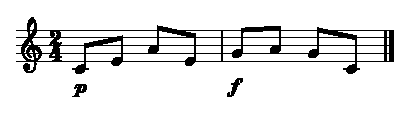
\includegraphics[width=0.7\textwidth]{chapters/cap-musica-basica/matiz1-1.eps}
\caption{Melodia com diferentes matizes.}
\label{fig:matiz1-1}
\end{figure}

Para aumentar ou diminuir gradativamente a intensidade do som,
também podem ser usados sinais ou palavras \cite[pp. 215]{medteoria} \cite[pp. 117]{mascarenhascurso}:
\begin{itemize}
\item Crescendo (cresc.); símbolo: $<$
\item Decrescendo (decresc.) ou diminuindo (dim.); símbolo: $>$
\end{itemize}

\begin{example}[Indicando matizes com letras:]
A Figura \ref{fig:matiz2-1} mostra uma melodia 
que usa em todo o primeiro compasso uma mudança gradual de matiz desde o ``piano'' ate o ``forte'',
e em todo o segundo compasso uma mudança gradual do matiz desde o ``forte'' ate o ``piano''.
\end{example}
\begin{figure}[!h]
\centering
 \includegraphics[width=0.7\textwidth]{chapters/cap-musica-basica/matiz2-1.eps}
\caption{Melodia com mudanças graduais de matizes.}
\label{fig:matiz2-1}
\end{figure}


%\PRLsep{Simbolos como sinais de intesidade}


%%%%%%%%%%%%%%%%%%%%%%%%%%%%%%%%%%%%%%%%%%%%%%%%%%%%%%%%%%%%%%%%%%%%%%%%%%%%%%%%
\section{Repetições}
\index{Música!Repetições}
\label{sec:repetitions}

\subsection{Repetições de compassos}
\index{Música!Repetições de compassos}
\label{sec:repetitions:compass}

É possivel expressar a repetição de um o mais compassos usando o simbolo $\%$ 
\cite[pp. 249]{medteoria} \cite[pp. 111]{mascarenhascurso}.
A Figura \ref{fig:repeat-bar1-1} mostra o uso de repetições para escrever de forma compacta uma melodia.
A Figura \ref{fig:repeat-bar2-1} mostra a forma expandida da melodia expressada na Figura \ref{fig:repeat-bar1-1}.
\begin{figure}[!h]
\centering
    \begin{subfigure}[b]{0.6\textwidth}
        \includegraphics[width=0.9\textwidth]{chapters/cap-musica-basica/repeat-bar1-1.eps}
        \caption{Forma compacta.}
        \label{fig:repeat-bar1-1}
    \end{subfigure}
    \begin{subfigure}[b]{0.6\textwidth}
        \includegraphics[width=0.9\textwidth]{chapters/cap-musica-basica/repeat-bar2-1.eps}
        \caption{Forma expandida.}
        \label{fig:repeat-bar2-1}
    \end{subfigure}
\caption{Uso de repetições de compassos.}
\label{fig:repeat-bar1}
\end{figure}


\subsection{Repetições de trechos musicais}
\index{Música!Repetições de trechos}
\label{sec:repetitions:manycompass}

\subsubsection{Ritonelo}
\index{Música!Ritonelo}
É possivel expressar a repetição de um trecho de música usando o ``ritnonelo'' 
que tem um simbolo ``$:|$'' \cite[pp. 237]{medteoria} \cite[pp. 168]{cardoso1973curso}.

\begin{example}[Uso de ritnonelo final:]Se temos uma melodia com compasses $A$, $B$ e $C$,
então estas duas formas são equivalentes:
\begin{itemize}
\item $A~B~C~:|$
\item $A~B~C~A~B~C$
\end{itemize}
\end{example}


\begin{example}[Uso de ritnonelo inicial final:]Se temos uma melodia com compasses $A$, $B$ e $C$,
então estas duas formas são equivalentes:
\begin{itemize}
\item $ A|:B~C:|$
\item $A~B~C~B~C$
\end{itemize}
\end{example}

A Figura \ref{fig:ritonelo1-1} mostra o uso de repetições para escrever de forma compacta uma melodia.
A Figura \ref{fig:ritonelo2-1} mostra a forma expandida da melodia expressada na Figura \ref{fig:ritonelo1-1}.
\begin{figure}[!h]
\centering
    \begin{subfigure}[b]{0.75\textwidth}
        \includegraphics[width=0.9\textwidth]{chapters/cap-musica-basica/ritonelo1-1.eps}
        \caption{Forma compacta.}
        \label{fig:ritonelo1-1}
    \end{subfigure}
    \begin{subfigure}[b]{0.75\textwidth}
        \includegraphics[width=0.9\textwidth]{chapters/cap-musica-basica/ritonelo2-1.eps}
        \caption{Forma expandida.}
        \label{fig:ritonelo2-1}
    \end{subfigure}
\caption{Uso de repetições de trechos de música.}
\label{fig:ritonelo1}
\end{figure}

\subsubsection{Ritonelo com expressoes de 1ra e 2da vez}
Se um trecho de musica deve ser repetido mas com um diferente final cada vez,
então deve ser usado a expressão ``1ra vez'' e ``2da vez''
\cite[pp. 239]{medteoria} \cite[pp. 169]{cardoso1973curso}.

A Figura \ref{fig:ritonelo-times1-1} mostra o uso de repetições para escrever de forma compacta uma melodia.
A Figura \ref{fig:ritonelo-times2-1} mostra a forma expandida da melodia expressada na Figura \ref{fig:ritonelo-times1-1}.
\begin{figure}[!h]
\centering
    \begin{subfigure}[b]{0.75\textwidth}
        \includegraphics[width=0.9\textwidth]{chapters/cap-musica-basica/ritonelo-times1-1.eps}
        \caption{Forma compacta.}
        \label{fig:ritonelo-times1-1}
    \end{subfigure}
    \begin{subfigure}[b]{0.75\textwidth}
        \includegraphics[width=0.9\textwidth]{chapters/cap-musica-basica/ritonelo-times2-1.eps}
        \caption{Forma expandida.}
        \label{fig:ritonelo-times2-1}
    \end{subfigure}
\caption{Uso de repetições de trechos de música com expressoes de vez.}
\label{fig:ritonelo-times1}
\end{figure}


%%%%%%%%%%%%%%%%%%%%%%%%%%%%%%%%%%%%%%%%%%%%%%%%%%%%%%%%%%%%%%%%%%%%%%%%%%%%%%%%




\chapterimage{chapter_head_flauta1.pdf} % Chapter heading image

\chapter{\textcolor{red}{Fundamentos de composição musical}}
Nas seguintes sub seções abordaremos alguns conceitos importantes para iniciar o estudo da dacomposição musical;
porem, não aprofundaremos demasiado em toda a teoria, 
devido a que as explicações mostradas aqui, estão
orientadas para um público interessado na dança, que necesita a principio
ferramentas para entender a musica e melhorar sua percepção musical. 


%%%%%%%%%%%%%%%%%%%%%%%%%%%%%%%%%%%%%%%%%%%%%%%%%%%%%%%%%%%%%%%%%%%%%%%%%%%%%%%%
%%%%%%%%%%%%%%%%%%%%%%%%%%%%%%%%%%%%%%%%%%%%%%%%%%%%%%%%%%%%%%%%%%%%%%%%%%%%%%%%
\section{Articulação}
\label{sub:Articulation}
\index{Música!Articulação}

Nas partituras podemos ver alguns símbolos, 
que o compositor coloca como indicação ao interprete,
para informar como as notas musicais devem ser executadas ou 
articuladas entre sim \cite[pp. 56]{alves2004teoria}.
%%%%%%%%%%%%%%%%%%%%%%%%%%%%%%%%%%%%%%%%%%%%%%%%%%%%%%%%%%%%%%%%%%%%%%%%%%%%%%%%
\subsection{Legato }
\label{subsec:Legato}
\index{Música!Legato}
O  ``legato'' é um símbolo  que indica uma ligadura de expressão entre as notas,
neste caso a informação que da ao compositor é que as
notas devem ser executadas sem interrupções e
criando uma mudança de tons gradual para passar de uma nota musical a outra \cite[pp. 56]{alves2004teoria} \cite[pp. 18]{holland2013music}.

\begin{example}
A Figura \ref{fig:legato1} mostra um exemplo de uso do legato. 
Alguns instrumentos podem facilmente articular um legato, por exemplo o violino.
\end{example}

\begin{figure}[h!]
\centering
\begin{abc}[name=abc-legato1,width=0.80\linewidth]
X: 1 % start of header
K: C % scale: C major
M: 2/4 %meter - compasso
 (G2 E2 | G1  A1  G1 E1 )|
\end{abc}
\caption{Melodia com notas que devem ser executadas de forma ligada.}
\label{fig:legato1}
\end{figure}

%%%%%%%%%%%%%%%%%%%%%%%%%%%%%%%%%%%%%%%%%%%%%%%%%%%%%%%%%%%%%%%%%%%%%%%%%%%%%%%%
\subsection{Staccato}
\label{subsec:Staccato}
\index{Música!Staccato}

O staccato é um símbolo, desenhado com um ponto (.), 
que indica a diminuição na \hyperref[sec:pos:Duracion]{\textbf{duração}} de uma nota (aproximadamente um 50\%), 
dando nela um efeito de separação ou destaque \cite[pp. 56]{alves2004teoria} \cite[pp. 16]{holland2013music}.

\begin{example}
A Figura \ref{fig:staccato1a} mostra um exemplo de uso do staccato. 
Na Figura \ref{fig:staccato1b} podemos ver uma escrita equivalente, sem o uso do símbolo de staccato.
\end{example}

\begin{figure}[h!]
\centering
\begin{subfigure}[c]{0.80\textwidth}
\begin{abc}[name=abc-staccato1a]
X: 1 % start of header
K: C % scale: C major
M: 2/4 %meter - compasso
 .G2 .E2 | .G1  .A1  .G1 .E1 | 
\end{abc}
\caption{Notação de notas musicais em staccato.}
\label{fig:staccato1a}
\end{subfigure}
~ %
\begin{subfigure}[c]{1.00\textwidth}
\begin{abc}[name=abc-staccato1b]
X: 1 % start of header
K: C % scale: C major
M: 2/4 %meter - compasso
 G1 z1 E1 z1 | G1/2 z1/2 A1/2 z1/2 G1/2 z1/2 E1/2 z1/2 | 
\end{abc}
\caption{Forma de execução de notas musicais em staccato.}
\label{fig:staccato1b}
\end{subfigure}
\caption{Melodia com notas que devem ser executadas em staccato.}
\label{fig:staccato1}
\end{figure}

\subsubsection{Staccatissimo}

O staccatissimo, staccato seco ou martelado é um símbolo, com uma função similar ao staccato;
porém indica uma diminuição maior na \hyperref[sec:pos:Duracion]{\textbf{duração}} 
de nota (aproximadamente ao 25\%) \cite[pp. 56]{alves2004teoria} \cite[pp. 16]{holland2013music}.

\begin{example}
A Figura \ref{fig:staccatissimo1a} mostra um exemplo de uso do staccatissimo. 
Na Figura \ref{fig:staccatissimo1b} podemos ver uma escrita equivalente, sem o uso do símbolo de staccatissimo.
\end{example}

\begin{figure}[h!]
\centering
\begin{subfigure}[c]{0.80\textwidth}
\begin{abc}[name=abc-staccatissimo1a]
X: 1 % start of header
K: C % scale: C major
M: 2/4 %meter - compasso
 !wedge!G2 !wedge!E2 | !wedge!G1  !wedge!A1  !wedge!G1 !wedge!E1 | 
\end{abc}
\caption{Notação de notas musicais em staccatissimo.}
\label{fig:staccatissimo1a}
\end{subfigure}
~ %
\begin{subfigure}[c]{1.00\textwidth}
\begin{abc}[name=abc-staccatissimo1b]
X: 1 % start of header
K: C % scale: C major
M: 2/4 %meter - compasso
 G1/2 z3/2 E1/2 z3/2 | G1/4 z3/4 A1/4 z3/4 G1/4 z3/4 E1/4 z3/4 | 
\end{abc}
\caption{Forma de execução de notas musicais em staccatissimo.}
\label{fig:staccatissimo1b}
\end{subfigure}
\caption{Melodia com notas que devem ser executadas em staccato.}
\label{fig:staccatissimo1}
\end{figure}

%%%%%%%%%%%%%%%%%%%%%%%%%%%%%%%%%%%%%%%%%%%%%%%%%%%%%%%%%%%%%%%%%%%%%%%%%%%%%%%%
\subsection{Tenuto}
\label{subsec:Tenuto}
\index{Música!Tenuto}

O tenuto (ou sostenuto) é um símbolo desenhado com uma linha reta (-)  
que indica que deve ser sustentada a 
\hyperref[sec:pos:Duracion]{\textbf{duração}} e a 
\hyperref[sec:pos:Intensidade]{\textbf{intensidade}} da nota ao máximo \cite[pp. 56]{alves2004teoria} \cite[pp. 17]{holland2013music}.

\begin{example}
A Figura \ref{fig:tenuto1} mostra um exemplo de uso do tenuto. 
\end{example}


\begin{figure}[h!]
\centering
\begin{abc}[name=abc-tenuto1,width=0.80\linewidth]
X: 1 % start of header
K: C % scale: C major
M: 2/4 %meter - compasso
 !tenuto!G2 !tenuto!E2 | !tenuto!G1  !tenuto!A1  !tenuto!G1 !tenuto!E1 |
\end{abc}
\caption{Melodia com notas que devem ser executadas de forma sustenido.}
\label{fig:tenuto1}
\end{figure}

%%%%%%%%%%%%%%%%%%%%%%%%%%%%%%%%%%%%%%%%%%%%%%%%%%%%%%%%%%%%%%%%%%%%%%%%%%%%%%%%
\subsection{Accénto}
\label{subsec:Accento}
\index{Música!Accénto}

O accénto é um símbolo desenhado com (>) 
que indica que a nota deve ser enfatizada; 
ou seja que a nota deve receber um aumento de \hyperref[sec:pos:Intensidade]{\textbf{intensidade}} \cite[pp. 56]{alves2004teoria}.

\begin{example}
A Figura \ref{fig:accento1} mostra um exemplo de uso do accénto.
Nela os tempos fracos tem um aumento de intensidade provocando \hyperref[sec:contratempo]{\textbf{contratempos}}. 
\end{example}


\begin{figure}[h!]
\centering
\begin{abc}[name=abc-accento1,width=0.80\linewidth]
X: 1 % start of header
K: C % scale: C major
M: 2/4 %meter - compasso
 G2 !>!E2 | G1  !>!A1  !>!G1 !>!E1 |
\end{abc}
\caption{Melodia com notas que devem ser executadas de forma sostenida.}
\label{fig:accento1}
\end{figure}
 


%%%%%%%%%%%%%%%%%%%%%%%%%%%%%%%%%%%%%%%%%%%%%%%%%%%%%%%%%%%%%%%%%%%%%%%%%%%%%%%%
\section{\textcolor{red}{Motivos}}
\index{Música!Motivos}
\index{Música!Motif}

%%%%%%%%%%%%%%%%%%%%%%%%%%%%%%%%%%%%%%%%%%%%%%%%%%%%%%%%%%%%%%%%%%%%%%%%%%%%%%%%
\section{\textcolor{red}{Frase}}\index{Música!Frase}
\cite[pp. 150]{medteoria}


A frase melódica
% https://pt.wikipedia.org/wiki/Frase_(música)
Frase rítmica
% rhythmic phrase
% https://books.google.com.br/books?id=KjSJcjIBvjcC&pg=PA5&dq=rhythmic+phrase&hl=es-419&sa=X&ved=0ahUKEwiqj6r-utrhAhV4E7kGHaO2AXAQ6AEIKTAA#v=onepage&q=rhythmic%20phrase&f=false
% https://en.wikipedia.org/wiki/Phrase_(music)
%%%%%%%%%%%%%%%%%%%%%%%%%%%%%%%%%%%%%%%%%%%%%%%%%%%%%%%%%%%%%%%%%%%%%%%%%%%%%%%%
\section{\textcolor{red}{Período}}\index{Música!Período}
% https://en.wikipedia.org/wiki/Period_(music)
%%%%%%%%%%%%%%%%%%%%%%%%%%%%%%%%%%%%%%%%%%%%%%%%%%%%%%%%%%%%%%%%%%%%%%%%%%%%%%%%
\section{\textcolor{red}{Sentencia}}\index{Música!Sentencia}
% https://en.wikipedia.org/wiki/Sentence_(music)
%%%%%%%%%%%%%%%%%%%%%%%%%%%%%%%%%%%%%%%%%%%%%%%%%%%%%%%%%%%%%%%%%%%%%%%%%%%%%%%%
\section{\textcolor{red}{Riff}}\index{Música!Riff}
% https://es.wikipedia.org/wiki/Riff

%%%%%%%%%%%%%%%%%%%%%%%%%%%%%%%%%%%%%%%%%%%%%%%%%%%%%%%%%%%%%%%%%%%%%%%%%%%%%%%%
\section{\textcolor{red}{Fraseio}}
\index{Música!Fraseio}

% https://es.wikipedia.org/wiki/Fraseo
% https://en.wikipedia.org/wiki/Musical_phrasing

%%%%%%%%%%%%%%%%%%%%%%%%%%%%%%%%%%%%%%%%%%%%%%%%%%%%%%%%%%%%%%%%%%%%%%%%%%%%%%%%
\section{\textcolor{red}{Cadencia}}
\index{Música!Cadencia}

\cite[pp. 111]{holst1998abc}

% https://es.wikipedia.org/wiki/Cadencia_(música)

% https://en.wikipedia.org/wiki/Cadence

cadencia harmonica \cite[pp. 67]{melcior1859diccionario} \cite[pp. 60]{pedrell2009diccionario}

cadencia melodica \cite[pp. 66]{melcior1859diccionario} \cite[pp. 60]{pedrell2009diccionario}



\chapterimage{chapter_head_2.pdf} % Chapter heading image

\chapter{\textcolor{blue}{Fundamentos de musicalidade na dança}}


%%%%%%%%%%%%%%%%%%%%%%%%%%%%%%%%%%%%%%%%%%%%%%%%%%%%%%%%%%%%%%%%%%%%%%%%%%%%%%%%
\section{\textcolor{green}{Contagem ritmica dos passos}}
Antes de iniciar esta seção é importante mencionar uma
problemática que é vista com muita frequência nas escolas de dança; 
esta é gerada devido a que: A forma em que os tempos são contados 
nos compassos, é
diferente à realizada entre profissionais da música e da dança. 
Sendo que a contagem dos profissionais da música segue as normas
e notações indicadas na partitura, e no caso de profissionais da dança segue geralmente um enfoque 
particular a cada escola de dança, visando só em muitos casos o fácil entendimento do aluno da
execução dos movimentos, e não uma rigorosidade teórica no uso de termos e 
expressões musicais.


\subsection{\textcolor{blue}{Percepção rítmica do ouvinte}}
Quando escutamos uma música, na qual é tipicamente dançado samba de gafieira,
podemos distinguir que a soma dos sonidos produzidos pelos instrumentos realizam 
um padrão de repetição muito particular, geralmente ligado dois onomatopeias: ``Chic Chic Tum'' ou ``tum Tum''.


A Figura \ref{fig:abc-caquarela} representa os compassos 18, 19 e 20 da  
composição musical ``Aquarela do Brasil'' escrita
por Ary Barroso em 1939 \cite{AquarelaDoBrasil}; 
a versão mostrada na figura teve arranjos por Irineu Krüger \cite{Irineu}. 
Nesta versão, a música está representada com 1 voz ou coro de voces (``Voice Choir'') e 4 
instrumentos (``Eb'',``Bb'',``Strings'' e ``D. Bass''), que usam uma 
formula de compasso $2/4$, de modo que cada compasso
é binário e
pode ser preenchido usando duas semínimas (2\quarternote).
\begin{figure}[ht]
\centering
%\includegraphics[width=\textwidth]{chapters/cap-fundamentos/aquarela.png}
\begin{abc}[name=abc-caquarela]
% abcm2ps aquarela.abc  -O aquarela.ps
% ps2epsi aquarela.ps aquarela.eps
%
X: 1 % start of header
T: Brazil - Aquarela do Brasil
C: Music: Ary Barroso, 1939
C: Arranged by: Irineu Krüger
K: C % scale: C major
M: 2/4 % formula do compasso
%
V:1 clef=treble name="Voice Choir" sname="Voice Choir"
V:2 clef=treble name="Eb" sname="Eb"
V:3 clef=treble name="Bb" sname="Bb"
V:4 clef=treble name="Strings" sname="Strings"
V:5 clef=bass   name="D. Bass" sname=""D. Bass"
%
%
[V:1] "18" C'3/2A/2C2  |"19" A3/2(G/2 G/2)E1E/2  |"20" z/2 C'1A/2 C'1C'1  |
w:    Ó Bras-sil        sam-ba_ que dá       bam-bo-leio_ 
w:    Ó Bras-sil        ver-de que dá_       pa-ra~o mun-do 
%
%
[V:2] G1z/2G1z/2G1  | G1z/2G1z/2G1  | G1z/2G1z/2G1  |
%
%
[V:3] z4  | z4  | z4  |
%
%
[V:4] G1z/2G1z/2G1  | G1z/2G1z/2G1  | G1z/2G1z/2G1  |
%
%
[V:5] C,2 G,,2  | C,1 z1 G,,2  | C,2 G,,2  |
\end{abc}
\caption{3 compassos da partitura da composição ``Aquarela do brasil''}
\label{fig:abc-caquarela}
\end{figure}

\subsubsection{Percepção do: Chic Chic Tum}
Analisando este fragmento de partitura e escutando a música produzida, 
podemos perceber que os instrumentos executados em conjunto geram um sonido identificável
com a onomatopeia ``Chic Chic Tum''.
Assim, o inicio de cada compasso coincide com o ``Tum''; 
sendo que este é o momento em que a maioria dos instrumentos produzem um sonido, 
de modo que a sensação para o ouvinte é de uma potencia sonora maior. 
Cada instrumento prolongará seu sonido de forma diferente; 
porem,  podemos dizer que: o ``Tum'' ocupa $1$ tempo (\quarternote), 
e que cada ``Chic'' ocupa médio tempo (0.5\quarternote),
sendo que o primeiro ``Chic'' é executado no tempo fraco de ``D. Bass'', 
e o segundo ``Chic'' solapa e obscurece ao  primeiro, 
sendo executado na parte fraca do tempo fraco de ``Strings'' ou ``Eb'' (é dizer, fazem contratempos);
conseguindo assim criar a ilusão do ``Chic Chic Tum'', com ``Chic''s de médio tempo ; de modo que:
\begin{equation}
Chic + Chic = Tum ~~ \Longleftrightarrow ~~ Chic = \frac{Tum}{2}.
\end{equation}
 
Por outro lado, se a percepção do ouvinte é mais
aguçada, poderá escutar ``a Chic Chic Tum''; 
neste caso, o sonido ``Tum'' é solapado por o sonido de ``a'',
quando transcorrido um $75\%$ do primeiro tempo do compasso; 
o sonido ``a''  se prolonga incluindo a parte forte do tempo fraco subsequente, 
este sonido é executado pelos instrumentos ``Eb'' e ``Strings'' e constitui uma sincopa \cite[pp. 143]{medteoria}.


Pelo exposto anteriormente, agora podemos simplificar a partitura para gerar um sonido com onomatopeia
``Chic Chic Tum'', como é mostrado na Figura \ref{fig:abc-contratempo1}.
Assim,
o instrumento 1 executa dois sonidos, de modo que o primeiro contribui ao sonido 
``Tum'' e o segundo sonido gera o segundo ``Chic'' do compasso; por outro lado,
o instrumento 2 executa um ritmo com um padrão
de repetição de dois sonidos ``Tum'' e ``Chic'', nesse ordem;
sendo que a nota executada no tempo forte produz um sonido mais agudo que a 
executada no tempo fraco, isto é assim para poder diferenciar melhor ambos tempos.
\begin{figure}[ht]
\centering
\begin{abc}[name=abc-contratempo1]
X: 1 % start of header
K: C % scale: C major
M:2/4
%T: Contratempo num compasso binário
V:1 clef=treble name="Instrumento 1" sname="Inst. 1"
V:2 clef=bass   name="Instrumento 2" sname="Inst. 2"
[V:1] " ""T/2"G1 " ""T/2"z1 " ""T/2"z1 " ""T/2"G1 | " ""T/2"G1 " ""T/2"z1 " ""T/2"z1 " ""T/2"G1  :|
w:    Tum                     Chic                  Tum                   Chic           
[V:2] "Tempo"C,2 "Tempo"G,,2  | "Tempo"C,2 "Tempo"G,,2  :|
w:    Tum       Chic         Tum       Chic            
\end{abc}
\caption{Padrão de repetição para gerar um sonido de onomatopeia ``Chic Chic Tum''.}
\label{fig:abc-contratempo1}
\end{figure}

Conhecido tudo isto, é fácil perceber como existe uma diference entre 
o que percebemos ao escutar uma música e a forma como esta é escrita na partitura;
pois como é visto na Figura \ref{fig:abc-contratempo1}, quando escrevemos
um sonido com um padrão de repetição na ordem ``Tum Chic Chic'', para o ouvinte é mais natural associar
este sonido com o padrão ``Chic Chic Tum'', devido a que \textbf{quando um ser humano fala, este usa a pausa
para denotar o final de uma palavra}. Da mesma forma, ao escutar uma música, traduzimos
que o sonido que tem um silencio maior apos ser executado marca o final do ciclo
do padrão de repetição. Assim, o que um músico vê ao ler uma partitura
é um padrão de repetição ``Tum Chic Chic'', sendo que  um
ouvinte interpretará de forma instintiva que o padrão é ``Chic Chic Tum ''.

\subsubsection{\textcolor{red}{Percepção do: Tum Tum}}

Analisando o fragmento de partitura, na Figura \ref{fig:abc-caquarela}, 
e tentando issolar o instrumento ``D. Bass'',
podemos perceber que este gera um sonido identificável com a onomatopeia ``tum Tum''.
Podemos ver na Figura \ref{fig:abc-contratempo1tumtum} estre instrumento isoladamente.
\begin{figure}[ht]
\centering
\begin{abc}[name=abc-contratempo1tumtum]
X: 1 % start of header
K: C % scale: C major
M:2/4
%T: Contratempo num compasso binário
V:1 clef=bass   name="D. Bass" sname="D. Bass"      
[V:1] "Tempo"C,2 "Tempo"G,,2  | "Tempo"C,2 "Tempo"G,,2  :|
w:    Tum       tum         Tum       tum            
\end{abc}
\caption{Padrão de repetição para gerar um sonido de onomatopeia ``tum Tum''.}
\label{fig:abc-contratempo1tumtum}
\end{figure}


\subsection{Contagem de 3 passos em 2 tempos}
Esta diferença na forma de perceber o inicio e o final do ciclo de repetição, 
leva a um problema quando se quer ser rigoroso na forma de contar os tempos nos compassos; 
por exemplo, na Tabela \ref{tab:ritmo1} 
podemos ver 4 formas distintas, que podem adotar as pessoas, 
para contar os tempos nos compassos indicando a distribuição de tempos, 
onde ``$T$'' representa um tempo do compasso.
\begin{table}[ht]
  \centering
  \begin{tabular}    {c|ccc|c}
    \hline
    Tipos de contagem       & $T/2$ & $T/2$   & $T$ & Recomendável?\\
    \hline
    Contagem 1: & Chic  & Chic  & Tum   & Sim\\
    Contagem 2: & 2     & e     & 1     & Sim\\ \hline
    Contagem 3: & Con   & tra  & Tempo & Não\\
    Contagem 4: & 1     & e     & 2     & Não\\
    Contagem 5: & 1     & 2     & 3     & Não\\
    \hline
  \end{tabular}
  \caption{Tipos de contagem na samba de gafieira.}
\label{tab:ritmo1}
\end{table}

As formas de contagem que recomendo são:
\begin{itemize}
\item \textbf{A contagem 1}, 
devido que a principio, pode ser usada sem aprofundar demasiado 
na notação musical, de modo que só precisa ser explicado que a duração de um 
``Tum'' é o dobro que um ``Chic'', e anexar que tipicamente veremos que o ``Tum''
acontece no tempo 1 do compasso; 
%de modo que outra contagem valida seria ``Tum Chic Chic''; 
porem, a contagem 1 não está restrita ao uso destas silabas (``Chic'' e ``Tum''), 
em geral esta contagem representa a quase qualquer padrão de repetição
que use duas silabas diferentes, como por exemplo os padrões: ``Ta Ta Kum'', ``Tic Tic Pa'', etc. 
Este tipo de contagem já é muito usada na pratica e na literatura, pois 
podemos achar variantes como ``Quick-Quick Slow'' (Rápido-Rápido Lento no idioma inglês)
ou ``Tic Tic Tum'' seguindo a notação usada por Perna no seu livro sobre samba de gafieira \cite[pp. 146]{perna2002samba}.
\item \textbf{A contagem 2}, segue a notação de tempos na partitura, este tipo de
contagem é coerente com a musica, porem precisa de uma major explicação, 
para pessoas não iniciadas na musica e a dança. Porem, isto não quer dizer que seu
entendimento seja complexo, e sim que precisa um investimento em horas de aula
um pouco major que a contagem 1.
Mesmo assim, devemos ter cuidado pois pode-se dar o caso que a partitura não tenha compassos binários 
e sim quaternários, com contagens ``2 e 3'' ``4 e 1'', 
criando este tipo de contagem mais caminhos onde podemos perder coerência com a contagem na partitura.
\end{itemize}

~\\

Por outro lado, entre as contagens que não recomendo estão:
\begin{itemize}
\item \textbf{A contagem 3} (``Con-tra Tempo''), 
devido a que o uso deste padrão pode confundir às pessoas que desconhecem 
a definição formal do termo contratempo \cite[pp. 16]{mascarenhascurso} \cite[pp. 36]{azevedocompor}, 
e levar a confusão de achar que um contratempo é só uma distribuição de 3 tempos, 
sendo um o dobro dos outros dois, em termos de tempos execução.
\item \textbf{A contagem 4} é não recomendada, devido a que como é visto nas Figuras 
\ref{fig:abc-caquarela} e \ref{fig:abc-contratempo1}, musicalmente a contagem estaria invertida,
dado que tipicamente o ``Tum'' se execute no tempo 1.

\item \textbf{A contagem 5} não é recomendada, 
por motivos similares aos apresentados para a contagem 4. 
Além do fato que os números atribuídos estão distantes da
notação verdadeira na partitura, mesmo sim esta houvesse sido escrita num compasso quaternário.
\end{itemize}

\subsection{\textcolor{red}{Contagem de 2 passos em 2 tempos}}


%%%%%%%%%%%%%%%%%%%%%%%%%%%%%%%%%%%%%%%%%%%%%%%%%%%%%%%%%%%%%%%%%%%%%%%%%%%%%%%%
\section{\textcolor{red}{Procurando um bom ``Timing''}}
Procurando o momento certo

 sincronização [https://www.infopedia.pt/dicionarios/ingles-portugues/timing]
 sentido de oportunidade [https://www.infopedia.pt/dicionarios/ingles-portugues/timing]
%%%%%%%%%%%%%%%%%%%%%%%%%%%%%%%%%%%%%%%%%%%%%%%%%%%%%%%%%%%%%%%%%%%%%%%%%%%%%%%%
\section{\textcolor{red}{Articulação das notas musicais vs. dança}}
Articulação das notas musicais refletido na nossa dança

Legato vs. sttacato

%%%%%%%%%%%%%%%%%%%%%%%%%%%%%%%%%%%%%%%%%%%%%%%%%%%%%%%%%%%%%%%%%%%%%%%%%%%%%%%%
\section{\textcolor{red}{Procurando o tempo forte da música}}
Tempo forte ou tempo 1

simples
\begin{itemize}
\item O tempo em que estatisticamente percebemos com maior potencia sonora. 
\item Se conseguimos identificar audivelmente um padrão de repetição ``Chick-Chick Tum'', o tum é o tempo forte
\item O tempo em que estatisticamente percebemos que o cantor  coloca o acento da palavra. 
\end{itemize}

complexos 
\begin{itemize}
\item Se percebemos um ``break'' da música com final de frase musical conclusivo 
(satisfatório, com uma sensação de ponto aparte), então este aconteceu no tempo forte.
\end{itemize}

%%%%%%%%%%%%%%%%%%%%%%%%%%%%%%%%%%%%%%%%%%%%%%%%%%%%%%%%%%%%%%%%%%%%%%%%%%%%%%%%
\section{\textcolor{red}{Dançando no tempo forte da música}}

Que significa dançar no tempo forte? 
pisar o tum  no tempo forte.

Se percebo que estou pisando no fraco como corrigir?
podemos usar
\begin{itemize}
\item Caminhada em contratempo
\item Fazemos balaços um número impar de vezes.
\end{itemize}


%%%%%%%%%%%%%%%%%%%%%%%%%%%%%%%%%%%%%%%%%%%%%%%%%%%%%%%%%%%%%%%%%%%%%%%%%%%%%%%%
\section{\textcolor{red}{Percebendo frases musicais}}

\subsection{\textcolor{red}{percebendo frases com final conclusivo}}
\subsection{\textcolor{red}{percebendo frases com final suspensivo}}
\subsubsection{\textcolor{red}{percebendo frases com final suspensivo a contratempo e sincopado}}

%%%%%%%%%%%%%%%%%%%%%%%%%%%%%%%%%%%%%%%%%%%%%%%%%%%%%%%%%%%%%%%%%%%%%%%%%%%%%%%%
\section{\textcolor{red}{Contando e medindo a frase musical}}
Provavelmente 4
\begin{itemize}
\item 4 compassos
\item 8 compassos
\item 2 compassos
\item 16 compassos
\end{itemize}

%%%%%%%%%%%%%%%%%%%%%%%%%%%%%%%%%%%%%%%%%%%%%%%%%%%%%%%%%%%%%%%%%%%%%%%%%%%%%%%%
\section{\textcolor{red}{Frase musical, Rap e musicalizar poesias}}
% https://scielo.conicyt.cl/scielo.php?script=sci_arttext&pid=S0719-32622018000100030

%%%%%%%%%%%%%%%%%%%%%%%%%%%%%%%%%%%%%%%%%%%%%%%%%%%%%%%%%%%%%%%%%%%%%%%%%%%%%%%%
\section{\textcolor{red}{Percebendo e usando o ``break'' da música}}




%%%%%%%%%%%%%%%%%%%%%%%%%%%%%%%%%%%%%%%%%%%%%%%%%%%%%%%%%%%%%%%%%%%%%%%%%%%%%%%%
\section{\textcolor{red}{Seguindo isoladamente os instrumentos}}
\begin{itemize}
\item Dançando choro-chorinho na melodia esquecendo o ``Chick-Chick Tum''.
\item Trabalhando com marionetas um em cada mão, ou dedo.
\item Cada aluno simula que tem um instrumento virtual e toca ele.
\end{itemize}

%%%%%%%%%%%%%%%%%%%%%%%%%%%%%%%%%%%%%%%%%%%%%%%%%%%%%%%%%%%%%%%%%%%%%%%%%%%%%%%%
\section{\textcolor{red}{Mickey mousing}}




%----------------------------------------------------------------------------------------
%----------------------------------------------------------------------------------------
%----------------------------------------------------------------------------------------
%	PART
%----------------------------------------------------------------------------------------
\part{Trabalhando de forma unipessoal}

%----------------------------------------------------------------------------------------
%	CHAPTER 
%----------------------------------------------------------------------------------------
\chapterimage{chapter_head_cris1.pdf} % Chapter heading image

\chapter{ \Footwork~ no samba de gafieira }

Uma parte muito importante do desenvolvimento na dança é o treino e a repetição;
nesse sentido, o dançarino muitas vezes tem que investir muito tempo 
de treinamento em sim mesmo, para desenvolver de forma fluida e natural seus movimentos.
Este é um trabalho duro e contínuo, que muitas vezes abordaremos de forma individual, 
e no nosso próprio tempo de aprendizagem; 
por isso é importante conhecer uma serie de exercícios que nos preparem,
fisicamente, e nos deem consciência corporal para executar nossos movimentos na dança.

Neste capítulo serão apresentados, uma serie de movimentos que podem ser usados,
no treinamento unipessoal; eles estão representados usando uma notação coreográfica
para o \footwork~(do inglês ``footwork'' ), que será previamente explicada.
 
\section{Notação coreográfica para o \footwork }
Para descrever o \footwork~ numa representação escrita, 
será usado uma notação baseada numa vista da posição dos pés no chão. 
Existirá uma representação para cada subdivisão temporal do movimento, 
estas subdivisões serão chamadas de tempos coreográficos, 
para diferenciar-lhos dos tempos do compasso; 
pois a duração e o inicio destes será diferente\footnote{Para 
mais detalhes da contagem dos tempos no compasso, ver Seção \ref{sec:Tempo}.}.

A Tabela \ref{tab:notationunipessoal} descreve o significado de todos os símbolos usados,
na notação coreográfica para o \footwork.
\begin{longtable}{| c |p{0.80\textwidth}  |}
  %\begin{tabular}{| p{0.1\textwidth}|p{0.80\textwidth}  |}
  \hline
  Símbolo & Descrição \\ \hline \hline 
  T & Abreviatura do termo \textbf{tempo}, se referindo ao tempo do compasso na música, ver Seção \ref{sec:Tempo}. \\ \hline

  TC & Abreviatura do termo \textbf{tempo coreográfico}, 
  de modo que cada movimento é subdividido temporalmente num número de TC. 
  Todos os TC são definidos na descrição de cada movimento, 
  tendo sempre neste âmbito a mesma duração;
  porém, este é um valor relativo ao tempo musical, e cada movimento pode usar um TC de 1, 1/2 ou 1/4 do tempo musical,
  procurando otimizar a didática na explicação do movimento. \\ \hline

  \raisebox{-\totalheight}{\includegraphics[width=1cm]{notation-foot/notacion1-seta.eps}} & A \textbf{seta} 
  indica o percorrido para que um pé chegue à posição do TC atual; ou seja nos fala do passado do TC.
  A cor pode variar em função se no final do movimento se chega com o peso do corpo. \\ \hline 

  \raisebox{-\totalheight}{\includegraphics[width=1cm]{notation-foot/notacion-box.eps}} & 
  O \textbf{quadro de trabalho} é onde se colocará a disposição dos pés no chão, em cada tempo coreográfico,
  de modo que esta disposição indica o estado no inicio do TC.  \\ \hline
  %Se consideramos ao \textbf{quadro de trabalho} um plano cartesiano a posição (0,0) é indicado com um símbolo de +.  \\ \hline

  \raisebox{-\totalheight}{\includegraphics[width=0.4cm]{notation-foot/notacion-plus.eps}} & 
  Este símbolo indica a \textbf{origem} ou posição (0,0), do plano cartesiano que representa o \textbf{quadro de trabalho};
  e pode ser colocado em qualquer lugar deste. \\ \hline

  \raisebox{-\totalheight}{\includegraphics[width=0.4cm]{notation-foot/notacion-plusc.eps}} & 
  Este símbolo indica a posição da \textbf{próxima origem} ou posição (0,0), 
  do plano cartesiano que representa \textbf{quadro de trabalho};
  isto será usado para descrever movimentos com deslocamentos longos.
  Este símbolo pode ser colocado em qualquer lugar do \textbf{quadro de trabalho}. \\ \hline

  \raisebox{-\totalheight}{\includegraphics[width=1cm]{notation-foot/notacion-box-dot.eps}} & 
  O \textbf{quadro de descanso} é um símbolo que indica que nesse tempo coreográfico não se realizará movimento de pés;
  desenhar este quadro é opcional, dado que se entende que se o quadro não está desenhado então não existe informação 
  de movimento nesse tempo, o único proposito é didático para melhorar a clareza das representações.  \\ \hline


  \raisebox{-\totalheight}{\includegraphics[height=1.2cm]{notation-foot/notacion-esq-preto.eps}} & Este símbolo 
  indica o \textbf{pé esquerdo}; 
  o calcanhar está desenhado com branco para indicar que essa parte do pé não deve suportar 
  o peso do corpo.
  A cor da parte dianteira do pé pode variar em função se este tiver o peso do corpo. \\ \hline  

  \raisebox{-\totalheight}{\includegraphics[height=1.2cm]{notation-foot/notacion-der-preto.eps}} & Este símbolo 
  indica o \textbf{pé direito}; 
  o calcanhar está desenhado com branco para indicar que essa parte do pé não deve suportar 
  o peso do corpo. 
  A cor da parte dianteira do pé pode variar em função se este tiver o peso do corpo. \\ \hline  

  \raisebox{-\totalheight}{\includegraphics[height=0.6cm]{notation-foot/notacion-esq-preto-ponta.eps}} & Este símbolo 
  indica que se usará a \textbf{ponta do pé esquerdo};
  a porção da ponta que será usada quedará a decisão de cada dançarino. 
  A cor pode variar em função se este pé tiver o peso do corpo. \\ \hline  

  \raisebox{-\totalheight}{\includegraphics[height=0.60cm]{notation-foot/notacion-der-preto-ponta.eps}} & Este símbolo 
  indica que se usará a \textbf{ponta do pé direito};
  a porção da ponta que será usada quedará a decisão de cada dançarino. 
  A cor pode variar em função se este pé tiver o peso do corpo. \\ \hline


  \raisebox{-\totalheight}{\includegraphics[width=1cm]{notation-foot/notacion-preto.eps}} & Os símbolos 
  com esta cor indicam que o pé ao que fazem referencia \textbf{tem o peso do corpo}. \\ \hline 

  \raisebox{-\totalheight}{\includegraphics[width=1cm]{notation-foot/notacion-gris.eps}} & Os símbolos 
  com esta cor indicam que o pé ao que fazem referencia \textbf{não tem o peso do corpo}. \\ \hline

  \raisebox{-\totalheight}{\includegraphics[width=1cm]{notation-foot/notacion-pica-pau.eps}} & 
  O símbolo \textbf{pica-pau} indica que não existe deslocamento e só levantaremos o pé
  e o colocaremos no mesmo lugar, este simbolo é usado quando esse pé não tem o peso do corpo.  \\ \hline

  \raisebox{-\totalheight}{\includegraphics[width=1cm]{notation-foot/notacion-quadril.eps}} & 
  A \textbf{bússola} indica um vetor paralelo à direção a qual deve apontar o quadril.
  O uso deste símbolo é opcional, e só é usado quando a informação do quadril é relevante
  para o exercício.   \\ \hline


  \raisebox{-\totalheight}{\includegraphics[width=1cm]{notation-foot/notacion-twist-antihorario.eps}} & 
  O símbolo indica um \textbf{twist} com o pé em sentido antihorário. \\ \hline 

  \raisebox{-\totalheight}{\includegraphics[width=1cm]{notation-foot/notacion-twist-horario.eps}} & 
  O símbolo indica um \textbf{twist} com o pé em sentido horário. \\ \hline

  %\end{tabular}
  \caption{Notação coreográfica para o \footwork.}
  \label{tab:notationunipessoal}
\end{longtable}

%\section{\textcolor{blue}{Movimentos para trabalhar de forma individual}}


Nas seguintes seções serão descritos uma serie de movimentos que poderão ser treinados individualmente.
Estes são interessantes para o desenvolvimento de consciência corporal, 
e poderão ser usados posteriormente na dança a dois,
fazendo algumas leves modificações ou adaptações.

\begin{tcbattention}
Nas próximas seções, é usado o termo \textbf{variante} para descrever aos movimentos,
pois existem varias de formas ou estilos de realizar cada passo de dança.
Assim, é difícil estabelecer um critério comum para apontar a forma oficial de cada movimento,
pelo que estes serão referenciados sempre como variantes. 
\end{tcbattention}
%%%%%%%%%%%%%%%%%%%%%%%%%%%%%%%%%%%%%%%%%%%%%%%%%%%%%%%%%%%%%%%%%%%%%%%%%%%%%%%%

\section{ \Variante: Trança}
\index{Passo!Trança}

A Figura \ref{fig:pessoaltranca} mostra os movimentos necessários para executar uma variante do passo chamado trança.
\begin{itemize}
\item Cada quadro de trabalho representa a posição dos pés em cada tempo coreográfico;
\item um tempo coreográfico tem uma duração igual a meio tempo musical.
\item A trança é um movimento que pode ser executado de forma cíclica, de modo que 
a sequencia de passos pode executar-se como: TC1, TC2, ..., TC7, TC8, TC1, ..., etc.  
Quantas vezes se considere necessário.
\end{itemize}
\begin{figure}[!h]
  \centering
    \includegraphics[width=\workboxsize]{chapters/cap-passos-footwork/tranca.eps}
\caption{Diagrama de tempos coreográficos para a trança, $T=2~TC$.}
\label{fig:pessoaltranca}
\end{figure}

A Figura \ref{fig:abc-pessoaltrancatc2} mostra o diagrama de tempos para realizar o movimento trança,
iniciando com o tempo forte da música.
\begin{figure}[!h]
  \centering
\begin{abc}[name=abc-pessoaltrancatc2,width=0.7\linewidth]
X: 1 % start of header
K: C stafflines=1 % scale: C major
M: 2/4 %meter - compasso
%Q:1/4=80
V:1 clef=perc stem=up name="Ritmo" sname="Ritmo"
V:2 clef=perc stem=up name="TC"    sname="TC"
[V:1] |: B2  B1  B1 | B2  B1  B1 :| 
w:       tum  tchic tchic tum tchic tchic 
w: ~ ~ ~ ~ ~ ~ 
%w: ~ ~ ~ ~ ~ ~ 
[V:2] |: B1  B1  B2   | B1 B1  B1  B1 :| 
w:       TC1 TC2  TC3   TC5 TC6 TC7 TC8
\end{abc}
\caption{Diagrama de tempos para a execução da trança.}
\label{fig:abc-pessoaltrancatc2}
\end{figure}

Dependendo do movimento ou passo, desde o qual entremos na trança, 
em alguns momentos faremos este movimento iniciando desde o tempo fraco da música; 
nesse contexto, a Figura \ref{fig:abc-pessoaltranca} mostra a distribuição de tempos para realizar 
este movimento.
\begin{figure}[!h]
  \centering
\begin{abc}[name=abc-pessoaltranca,width=0.7\linewidth]
X: 1 % start of header
K: C stafflines=1 % scale: C major
M: 2/4 %meter - compasso
%Q:1/4=80
V:1 clef=perc stem=up name="Ritmo" sname="Ritmo"
V:2 clef=perc stem=up name="TC"    sname="TC"
[V:1] |: B2  B1  B1 | B2  B1  B1 :| 
w:       ~   tchic tchic tum tchic tchic 
w:       tum ~     ~     ~   ~     ~    
w: ~ ~ ~ ~ ~ ~ 
%w: ~ ~ ~ ~ ~ ~ 
[V:2] |: B1  B1  B1  B1 | B2  B1  B1 :| 
w:       ~   ~   TC1 TC2  TC3 TC5 TC6 
%w:       ~ ~ ~ ~   ~ ~ ~ ~ 
w:       TC7 TC8  ~  ~    ~       ~   ~    
\end{abc}
\caption{Diagrama de tempos para a execução da trança.}
\label{fig:abc-pessoaltranca}
\end{figure}


\begin{figure}[H]
  \centering
    \includegraphics[width=\textwidth]{steampunk1.eps}
\end{figure}
%%%%%%%%%%%%%%%%%%%%%%%%%%%%%%%%%%%%%%%%%%%%%%%%%%%%%%%%%%%%%%%%%%%%%%%%%%%%%%%%
\section{\Variante: Samba no pé}
\index{Passo!Samba no pé}

A Figura \ref{fig:pessoa-samba-no-pe} mostra os movimentos necessários para executar uma variante do passo de samba no pé para atrás.
\begin{itemize}
\item Cada quadro de trabalho representa a posição dos pés em cada tempo coreográfico;
\item um tempo coreográfico tem uma duração igual a meio tempo musical (T).
\item O passo básico de samba no pé  pode ser executado de forma cíclica, de modo que 
a sequencia de passos pode executar-se como: TC1, TC2, ..., TC7, TC8, TC1, ..., etc.  
Quantas vezes se considere necessário.
\end{itemize}
\begin{figure}[!h]
  \centering
    \includegraphics[width=\workboxsize]{chapters/cap-passos-footwork/samba-no-pe.eps}
\caption{Diagrama de tempos coreográficos para o passo de samba no pé  para atrás, $T=2~TC$.}
\label{fig:pessoa-samba-no-pe}
\end{figure}


A Figura \ref{fig:abc-pessoalsambape1} mostra o diagrama de tempos coreográficos para realizar o passo de samba no pé,
pra adiante.
\begin{figure}[!h]
  \centering
\begin{abc}[name=abc-pessoalsambape1,width=0.7\linewidth]
X: 1 % start of header
K: C stafflines=1 % scale: C major
M: 2/4 %meter - compasso
%Q:1/4=80
V:1 clef=perc stem=up name="Ritmo" sname="Ritmo"
V:2 clef=perc stem=up name="TC"    sname="TC"
[V:1] |: B2  B1  B1 | B2  B1  B1 :| 
w:       ~  tchic tchic tum tchic tchic 
w: tum ~ ~ ~ ~ ~ 
w: ~ ~ ~ ~ ~ ~ 
[V:2] |: B2  B1  B1 | B2  B1  B1 :| 
w:       ~   TC1 TC2  TC3 TC5 TC6 
w:       TC7  
\end{abc}
\caption{Diagrama de tempos para a execução do passo do samba no pé para atrás.}
\label{fig:abc-pessoalsambape1}
\end{figure}

%%%%%%%%%%%%%%%%%%%%%%%%%%%%%%%%%%%%%%%%%%%%%%%%%%%%%%%%%%%%%%%%%%%%%%%%%%%%%%%%

\section{\Variante~2: Samba no pé}\index{Passo!Samba no pé}

A Figura \ref{fig:pessoa-samba-no-pe-b} mostra os movimentos necessários para executar uma variante do passo de samba no pé para atrás.
\begin{itemize}
\item Cada quadro de trabalho representa a posição dos pés em cada tempo coreográfico;
\item um tempo coreográfico tem uma duração igual a meio tempo musical (T).
\item O passo básico de samba no pé  pode ser executado de forma cíclica, de modo que 
a sequencia de passos pode executar-se como: TC1, TC2, ..., TC7, TC8, TC1, ..., etc.  
Quantas vezes se considere necessário.
\end{itemize}

\begin{figure}[!h]
  \centering
    \includegraphics[width=\workboxsize]{chapters/cap-passos-footwork/samba-no-pe-b.eps}
\caption{Diagrama de tempos coreográficos para o passo de samba no pé  para atrás, $T=2~TC$.}
\label{fig:pessoa-samba-no-pe-b}
\end{figure}


A Figura \ref{fig:abc-pessoalsambape2} mostra o diagrama de tempos coreográficos para realizar a variante do passo de samba no pé,
pra atrás, explicada na Figura \ref{fig:pessoa-samba-no-pe-b}.
\begin{figure}[!h]
  \centering
\begin{abc}[name=abc-pessoalsambape2,width=0.7\linewidth]
X: 1 % start of header
K: C stafflines=1 % scale: C major
M: 2/4 %meter - compasso
%Q:1/4=80
V:1 clef=perc stem=up name="Ritmo" sname="Ritmo"
V:2 clef=perc stem=up name="TC"    sname="TC"
[V:1] |: B2  B1  B1 | B2  B1  B1 :| 
w:       ~  tchic tchic tum tchic tchic 
w: tum ~ ~ ~ ~ ~ 
w: ~ ~ ~ ~ ~ ~ 
[V:2] |: B2  B1  B1 | B2  B1  B1 :| 
w:       ~   TC1 TC2  TC3 TC5 TC6 
w:       TC7  
\end{abc}
\caption{Diagrama de tempos para a execução do passo do samba no pé para atrás.}
\label{fig:abc-pessoalsambape2}
\end{figure}

%%%%%%%%%%%%%%%%%%%%%%%%%%%%%%%%%%%%%%%%%%%%%%%%%%%%%%%%%%%%%%%%%%%%%%%%%%%%%%%%

\section{\Variante: Samba no pé (para adiante)}\index{Passo!Samba no pé para adiante}
A Figura \ref{fig:pessoa-samba-no-pe-adiante} mostra os movimentos necessários para executar uma variante do passo de samba no pé para adiante.
\begin{itemize}
\item Cada quadro de trabalho representa a posição dos pés em cada tempo coreográfico;
\item um tempo coreográfico tem uma duração igual a meio tempo musical (T).
\item O passo básico de samba no pé  pode ser executado de forma cíclica, de modo que 
a sequencia de passos pode executar-se como: TC1, TC2, ..., TC7, TC8, TC1, ..., etc.  
Quantas vezes se considere necessário.
\end{itemize}

\begin{figure}[!h]
  \centering
    \includegraphics[width=\workboxsize]{chapters/cap-passos-footwork/samba-no-pe-adiante.eps}
\caption{Diagrama de tempos coreográficos para o passo de samba no pé para adiante, $T=2~TC$.}
\label{fig:pessoa-samba-no-pe-adiante}
\end{figure}



A Figura \ref{fig:abc-pessoalsambape-adiante1} mostra o diagrama de tempos coreográficos para realizar o passo de samba no pé,
pra adiante.
\begin{figure}[!h]
  \centering
\begin{abc}[name=abc-pessoalsambape-adiante1,width=0.7\linewidth]
X: 1 % start of header
K: C stafflines=1 % scale: C major
M: 2/4 %meter - compasso
%Q:1/4=80
V:1 clef=perc stem=up name="Ritmo" sname="Ritmo"
V:2 clef=perc stem=up name="TC"    sname="TC"
[V:1] |: B2  B1  B1 | B2  B1  B1 :| 
w:       ~  tchic tchic tum tchic tchic 
w: tum ~ ~ ~ ~ ~ 
w: ~ ~ ~ ~ ~ ~ 
[V:2] |: B2  B1  B1 | B2  B1  B1 :| 
w:       ~   TC1 TC2  TC3 TC5 TC6 
w:       TC7  
\end{abc}
\caption{Diagrama de tempos para a execução do passo do samba no pé para atrás.}
\label{fig:abc-pessoalsambape-adiante1}
\end{figure}

%%%%%%%%%%%%%%%%%%%%%%%%%%%%%%%%%%%%%%%%%%%%%%%%%%%%%%%%%%%%%%%%%%%%%%%%%%%%%%%%

\section{\Variante~2: Samba no pé (para adiante)}\index{Passo!Samba no pé para adiante}
A Figura \ref{fig:pessoa-samba-no-pe-adiante-b} mostra os movimentos necessários para executar uma variante do passo de samba no pé para adiante.
\begin{itemize}
\item Cada quadro de trabalho representa a posição dos pés em cada tempo coreográfico;
\item um tempo coreográfico tem uma duração igual a meio tempo musical (T).
\item O passo básico de samba no pé  pode ser executado de forma cíclica, de modo que 
a sequencia de passos pode executar-se como: TC1, TC2, ..., TC7, TC8, TC1, ..., etc.  
Quantas vezes se considere necessário.
\end{itemize}


\begin{figure}[!h]
  \centering
    \includegraphics[width=\workboxsize]{chapters/cap-passos-footwork/samba-no-pe-adiante-b.eps}
\caption{Diagrama de tempos coreográficos para o passo de samba no pé para adiante, $T=2~TC$.}
\label{fig:pessoa-samba-no-pe-adiante-b}
\end{figure}


A Figura \ref{fig:abc-pessoalsambape-adiante2} mostra o diagrama de tempos coreográficos para realizar a variante do passo de samba no pé,
pra adiante, explicada na Figura \ref{fig:pessoa-samba-no-pe-adiante-b}.

\begin{figure}[!h]
  \centering
\begin{abc}[name=abc-pessoalsambape-adiante2,width=0.7\linewidth]
X: 1 % start of header
K: C stafflines=1 % scale: C major
M: 2/4 %meter - compasso
%Q:1/4=80
V:1 clef=perc stem=up name="Ritmo" sname="Ritmo"
V:2 clef=perc stem=up name="TC"    sname="TC"
[V:1] |: B2  B1  B1 | B2  B1  B1 :| 
w:       ~  tchic tchic tum tchic tchic 
w: tum ~ ~ ~ ~ ~ 
w: ~ ~ ~ ~ ~ ~ 
[V:2] |: B2  B1  B1 | B2  B1  B1 :| 
w:       ~   TC1 TC2  TC3 TC5 TC6 
w:       TC7  
\end{abc}
\caption{Diagrama de tempos para a execução do passo do samba no pé para adiante.}
\label{fig:abc-pessoalsambape-adiante2}
\end{figure}

%%%%%%%%%%%%%%%%%%%%%%%%%%%%%%%%%%%%%%%%%%%%%%%%%%%%%%%%%%%%%%%%%%%%%%%%%%%%%%%%
% da tesoura dupla

\section{ \Variante: Tesoura }\index{Passo!Tesoura}


A Figura \ref{fig:pessoa-tesoura} mostra os movimentos necessários para executar uma variante do passo chamado tesoura.
\begin{itemize}
\item Cada quadro de trabalho representa a posição dos pés em cada tempo coreográfico.
\item Um tempo coreográfico (TC) tem uma duração igual a meio tempo musical (T).
\item O passo básico de samba no pé  pode ser executado de forma cíclica, de modo que 
a sequencia de passos pode executar-se como: TC1, TC2, TC1, TC2, ..., etc.  
Quantas vezes se considere necessário.
\end{itemize}

\begin{figure}[!h]
  \centering
    \includegraphics[width=\workboxsize]{chapters/cap-passos-footwork/tesoura.eps}
\caption{Diagrama de tempos coreográficos para o passo tesoura, $T=2~TC$.}
\label{fig:pessoa-tesoura}
\end{figure}




A Figura \ref{fig:abc-pessoaltesoura} mostra o diagrama de tempos coreográficos para realizar a variante do passo de samba no pé,
pra adiante, explicada na Figura \ref{fig:pessoa-tesoura}.

\begin{figure}[!h]
  \centering
\begin{abc}[name=abc-pessoaltesoura,width=0.7\linewidth]
X: 1 % start of header
K: C stafflines=1 % scale: C major
M: 2/4 %meter - compasso
%Q:1/4=80
V:1 clef=perc stem=up name="Ritmo" sname="Ritmo"
V:2 clef=perc stem=up name="TC"    sname="TC"
[V:1] |: B2 B1    B1    | B2  B1    B1  :| 
w:       ~  tchic tchic   ~   tchic tchic
w:       tum ~    ~       tum ~ ~ 
w: ~ ~ ~ ~ ~ ~ 
[V:2] |: B2  B3/2  B1/2  | B2  B3/2  B1/2  :| 
w:       ~   TC1   TC2.5   ~   TC1   TC2.5 
w:       TC3 ~     ~       TC3  
\end{abc}
\caption{Diagrama de tempos para a execução do passo tesoura.}
\label{fig:abc-pessoaltesoura}
\end{figure}

%%%%%%%%%%%%%%%%%%%%%%%%%%%%%%%%%%%%%%%%%%%%%%%%%%%%%%%%%%%%%%%%%%%%%%%%%%%%%%%%

\section{\Variante: Balança corre corre}\index{Passo!Balança corre corre}


A Figura \ref{fig:pessoa-balanca-corre-corre} mostra os movimentos necessários para executar uma variante do passo chamado balança corre corre.
\begin{itemize}
\item Cada quadro de trabalho representa a posição dos pés em cada tempo coreográfico.
\item Um tempo coreográfico (TC) tem uma duração igual a meio tempo musical (T).
\item O passo básico de samba no pé  pode ser executado de forma cíclica, de modo que 
a sequencia de passos pode executar-se como: TC1, TC2, ..., TC5, TC6, TC1, TC2, ..., etc.  
Quantas vezes se considere necessário.
\end{itemize}

\begin{figure}[!h]
  \centering
    \includegraphics[width=\workboxsize]{chapters/cap-passos-footwork/balanca-corre-corre.eps}
\caption{Diagrama de tempos coreográficos para o passo balança corre corre, $T=2~TC$.}
\label{fig:pessoa-balanca-corre-corre}
\end{figure}




A Figura \ref{fig:abc-pessoal-balanca-corre-corre} mostra o diagrama de tempos coreográficos para realizar a variante do passo balanca corre corre,
explicada na Figura \ref{fig:pessoa-balanca-corre-corre}.

\begin{figure}[!h]
  \centering
\begin{abc}[name=abc-pessoal-balanca-corre-corre,width=1.0\linewidth]
X: 1 % start of header
K: C stafflines=1 % scale: C major
M: 2/4 %meter - compasso
%Q:1/4=80
V:1 clef=perc stem=up name="Ritmo" sname="Ritmo"
V:2 clef=perc stem=up name="TC"    sname="TC"
[V:1] |: B2 B1    B1    | B2  B1    B1   | B2  B1    B1 :| 
w:       ~  tchic tchic   tum tchic tchic  ~   ~     ~
w:       tum ~    ~       ~   ~     ~      tum tchic tchic
w: ~ ~ ~ ~ ~ ~ 
[V:2] |: B2  B1  B1   | B3/2 B1/2  B2    | B1  B1  B3/2 B1/2   :| 
w:       ~   TC1 TC2    TC3  TC4.5 TC5     ~   ~   ~    ~  
w:       TC5 ~   ~      ~    ~     ~       TC1 TC2 TC3  TC4.5
\end{abc}
\caption{Diagrama de tempos para a execução do passo balança corre corre.}
\label{fig:abc-pessoal-balanca-corre-corre}
\end{figure}

%%%%%%%%%%%%%%%%%%%%%%%%%%%%%%%%%%%%%%%%%%%%%%%%%%%%%%%%%%%%%%%%%%%%%%%%%%%%%%%%

\section{ \Variante: Pica-pau }
\index{Passo!Pica-pau}

A Figura \ref{fig:pessoa-pica-pau} mostra os movimentos necessários para executar uma variante do passo chamado pica-pau.
\begin{itemize}
\item Cada quadro de trabalho representa a posição dos pés em cada tempo coreográfico.
\item Um tempo coreográfico (TC) tem uma duração igual a meio tempo musical (T).
\item O passo básico de samba no pé  pode ser executado de forma cíclica, de modo que 
a sequencia de passos pode executar-se como: TC1, TC2, ..., TC7, TC8, TC1, TC2, ..., etc.  
Quantas vezes se considere necessário.
\end{itemize}

\begin{figure}[!h]
  \centering
    \includegraphics[width=\workboxsize]{chapters/cap-passos-footwork/pica-pau.eps}
\caption{Diagrama de tempos coreográficos para o passo pica-pau, $T=2~TC$.}
\label{fig:pessoa-pica-pau}
\end{figure}




A Figura \ref{fig:abc-pessoal-pica-pau} mostra o diagrama de tempos coreográficos para realizar o passo pica-pau,
explicada na Figura \ref{fig:pessoa-pica-pau}.

\begin{figure}[!h]
  \centering
\begin{abc}[name=abc-pessoal-pica-pau,width=0.6\linewidth]
X: 1 % start of header
K: C stafflines=1 % scale: C major
M: 2/4 %meter - compasso
%Q:1/4=80
V:1 clef=perc stem=up name="Ritmo" sname="Ritmo"
V:2 clef=perc stem=up name="TC"    sname="TC"
[V:1] |: B2  B1  B1 | B2  B1  B1 :| 
w:       ~  tchic tchic tum tchic tchic 
w: tum ~ ~ ~ ~ ~ 
w: ~ ~ ~ ~ ~ ~ 
[V:2] |: B2  B1  B1 | B2  B1  B1 :| 
w:       ~   TC1 TC2  TC3 TC5 TC6 
w:       TC7  
\end{abc}
\vspace{-20pt}
\caption{Diagrama de tempos para a execução do passo pica-pau.}
\label{fig:abc-pessoal-pica-pau}
\end{figure}



%%%%%%%%%%%%%%%%%%%%%%%%%%%%%%%%%%%%%%%%%%%%%%%%%%%%%%%%%%%%%%%%%%%%%%%%%%%%%%%%

\section{\Variante: Escovinha (para adiante)}
\index{Passo!Escovinha para adiante}

A Figura \ref{fig:abc-pessoalescovinha2} mostra o diagrama de tempos coreográficos para realizar o passo escovinha,
para adiante, os movimentos nos tempos coreográficos serão explicados na Figura \ref{fig:pessoalescovinha2}.

\begin{figure}[!h]
  \centering
\begin{abc}[name=abc-pessoalescovinha2,width=1.0\linewidth]
X: 1 % start of header
K: C stafflines=1 % scale: C major
M: 2/4 %meter - compasso
%Q:1/4=80
V:1 clef=perc stem=up name="Ritmo" sname="Ritmo"
V:2 clef=perc stem=up name="TC"    sname="TC"
[V:1] |: B2  B1  B1 | B2  B1  B1 :| 
w:       ~  tchic tchic tum tchic tchic 
w: tum ~ ~ ~ ~ ~ 
w: ~ ~ ~ ~ ~ ~ 
[V:2] |: B3/2 B1/2 B1/2  B1/2  B1/2 B1/2 | B3/2 B1/2  B1/2 B1/2  B1/2 B1/2 :| 
w:       ~   ~     TC1   TC1.5 TC2  TC2.5  TC3  TC4.5 TC5  TC5.5 TC6  TC6.5 
w:       TC7 TC8.5
\end{abc}
\caption{Diagrama de tempos para a execução do passo escovinha para adiante.}
\label{fig:abc-pessoalescovinha2}
\end{figure}


A Figura \ref{fig:pessoalescovinha2} mostra o diagrama de tempos coreográficos para realizar o passo escovinha, para adiante.
\begin{itemize}
\item Cada quadro de trabalho representa a posição dos pés em cada tempo coreográfico.
\item Um tempo coreográfico (TC) tem uma duração igual a meio tempo musical (T).
\item O passo básico de samba no pé  pode ser executado de forma cíclica, de modo que 
a sequencia de passos pode executar-se como: TC1, TC2, ..., TC7, TC8, TC1, ..., etc.  
Quantas vezes se considere necessário.
\end{itemize}


\begin{sidewaysfigure}[!h]
  \centering
    \includegraphics[width=\textwidth]{chapters/cap-passos-footwork/escovinha2.eps}
\caption{Diagrama detalhado de tempos coreográficos para a escovinha, $T=2~TC$.}
\label{fig:pessoalescovinha2}
\end{sidewaysfigure}


%%%%%%%%%%%%%%%%%%%%%%%%%%%%%%%%%%%%%%%%%%%%%%%%%%%%%%%%%%%%%%%%%%%%%%%%%%%%%%%%

\section{\Variante: Escovinha (para atrás)}
\index{Passo!Escovinha pra atrás}


A Figura \ref{fig:abc-pessoalescovinha2tras} mostra o diagrama de tempos para realizar uma variante do passo escovinha,
para atrás, os movimentos nos tempos coreográficos serão explicados na Figura \ref{fig:pessoalescovinha2tras}.


A Figura \ref{fig:pessoalescovinha2tras} mostra o diagrama de tempos coreográficos coreográficos para realizar o passo escovinha, para atrás.
\begin{itemize}
\item Cada quadro de trabalho representa a posição dos pés em cada tempo coreográfico.
\item Um tempo coreográfico (TC) tem uma duração igual a meio tempo musical (T).
\item O passo básico de samba no pé  pode ser executado de forma cíclica, de modo que 
a sequencia de passos pode executar-se como: TC1, TC2, ..., TC7, TC8, TC1, ..., etc.  
Quantas vezes se considere necessário.
\end{itemize}

\begin{sidewaysfigure}[h]
  \centering
\begin{subfigure}{0.65\textwidth}
\begin{abc}[name=abc-pessoalescovinha2tras,width=1.0\linewidth]
X: 1 % start of header
K: C stafflines=1 % scale: C major
M: 2/4 %meter - compasso
%Q:1/4=80
V:1 clef=perc stem=up name="Ritmo" sname="Ritmo"
V:2 clef=perc stem=up name="TC"    sname="TC"
[V:1] |: B2  B1  B1 | B2  B1  B1 :| 
w:       ~  tchic tchic tum tchic tchic 
w: tum ~ ~ ~ ~ ~ 
w: ~ ~ ~ ~ ~ ~ 
[V:2] |: B3/2 B1/2 B1/2  B1/2  B1/2 B1/2 | B3/2 B1/2  B1/2 B1/2  B1/2 B1/2 :| 
w:       ~   ~     TC1   TC1.5 TC2  TC2.5  TC3  TC4.5 TC5  TC5.5 TC6  TC6.5 
w:       TC7 TC8.5
\end{abc}
\vspace{-10pt}
\caption{Diagrama de tempos para a execução do passo escovinha para atrás.}
\label{fig:abc-pessoalescovinha2tras}
\end{subfigure}

\vspace{20pt}

\begin{subfigure}{\textwidth}
    \includegraphics[width=\textwidth]{chapters/cap-passos-footwork/escovinha2tras.eps}
    \caption{Diagrama detalhado de tempos coreográficos para a escovinha para atrás, $T=2~TC$.}
    \label{fig:pessoalescovinha2tras}
\end{subfigure}
\end{sidewaysfigure}



%%%%%%%%%%%%%%%%%%%%%%%%%%%%%%%%%%%%%%%%%%%%%%%%%%%%%%%%%%%%%%%%%%%%%%%%%%%%%%%%
\clearpage
\section{ \Variante: Escovinha trocando de lados}
\index{Passo!Escovinha trocando de lados}


A Figura \ref{fig:pessoa-escovinha-ambos-lados} mostra os movimentos necessários para executar uma variante do passo chamado pica-pau.
\begin{itemize}
\item Cada quadro de trabalho representa a posição dos pés em cada tempo coreográfico.
\item Um tempo coreográfico (TC) tem uma duração igual a meio tempo musical (T).
\item O passo básico de samba no pé  pode ser executado de forma cíclica, de modo que 
a sequencia de passos pode executar-se como: TC1, TC2, ..., TC7, TC8, TC1, TC2, ..., etc.  
Quantas vezes se considere necessário.
\end{itemize}

\begin{figure}[!h]
  \centering
    \includegraphics[width=\workboxsize]{chapters/cap-passos-footwork/escovinha-ambos-lados.eps}
\caption{Diagrama de tempos coreográficos para o passo escovinha intercambiando lados, $T=2~TC$.}
\label{fig:pessoa-escovinha-ambos-lados}
\end{figure}


A Figura \ref{fig:abc-pessoal-escovinha-ambos-lados} mostra o diagrama de tempos coreográficos para realizar o passo escovinha intercambiando lados,
explicada na Figura \ref{fig:pessoa-escovinha-ambos-lados}.

\begin{figure}[!h]
  \centering
\begin{abc}[name=abc-pessoal-escovinha-ambos-lados,width=0.55\linewidth]
X: 1 % start of header
K: C stafflines=1 % scale: C major
M: 2/4 %meter - compasso
%Q:1/4=80
V:1 clef=perc stem=up name="Ritmo" sname="Ritmo"
V:2 clef=perc stem=up name="TC"    sname="TC"
[V:1] |: B2  B1  B1 | B2  B1  B1 :| 
w:       ~  tchic tchic tum tchic tchic 
w: tum ~ ~ ~ ~ ~ 
w: ~ ~ ~ ~ ~ ~ 
[V:2] |: B2  B1  B1 | B2  B1  B1 :| 
w:       ~   TC1 TC2  TC3 TC5 TC6 
w:       TC7  
\end{abc}
\vspace{-20pt}
\caption{Diagrama de tempos para a execução do passo escovinha intercambiando lados.}
\label{fig:abc-pessoal-escovinha-ambos-lados}
\end{figure}


%%%%%%%%%%%%%%%%%%%%%%%%%%%%%%%%%%%%%%%%%%%%%%%%%%%%%%%%%%%%%%%%%%%%%%%%%%%%%%%%
\begin{comment}
\section{\textcolor{red}{\Variante: Pescaria}}\index{Passo!Pescaria}
\end{comment}

%%%%%%%%%%%%%%%%%%%%%%%%%%%%%%%%%%%%%%%%%%%%%%%%%%%%%%%%%%%%%%%%%%%%%%%%%%%%%%%%
\begin{comment}
\section{\textcolor{red}{\Variante: Puladinho}}\index{Passo!Puladinho}
\end{comment}




%----------------------------------------------------------------------------------------
%----------------------------------------------------------------------------------------
%----------------------------------------------------------------------------------------
%	PART
%----------------------------------------------------------------------------------------
\part{Notação da partitura de movimento}

\chapter{\textcolor{blue}{Posturas estruturais do movimento}}\index{Posturas}
As posturas estruturais do movimento ou simplesmente posturas, 
são posições estáticas do corpo, 
que aparecem naturalmente quando realizamos movimentos de samba de gafieira.
 

Para a explicação das posturas, neste capítulo, serão usados dois tipos diferentes de vista de câmera;
uma vista é frontal à pessoa, 
que representa a visão desde o ponto de vista do par de dança colocado ao frente a onde aponta o quadril do executante do movimento; 
e outra câmera com vista lateral, 
que representa a vista de um observador externo situado ao lado direito do executante do movimento, em relação ao quadril; 
conforme o descrito na Figura \ref{fig:vistacamera}.
Em todas as figuras está colorida a perna esquerda com a cor cinza, e a perna direita com um cor preto;
o triangulo $\triangle$ indica o lugar ou o pé onde está projetado o peso do corpo.
\begin{figure}[h]
  \centering
    \includegraphics[width=0.5\textwidth]{chapters/cap-partituramov-posturas/vistas.eps}
  \caption{Descrição da posição das câmeras nas vistas usadas nas imagens mostradas neste capítulo.}
  \label{fig:vistacamera}
\end{figure}

\begin{tcbinformation}
 Os nomes atribuídas as posturas expostas neste capítulo, 
 são definições com propósitos didáticos feitas explicitamente para este livro.
\end{tcbinformation}


%%%%%%%%%%%%%%%%%%%%%%%%%%%%%%%%%%%%%%%%%%%%%%%%%%%%%%%%%%%%%%%%%%%%%%%%%%%%%%%%
%%%%%%%%%%%%%%%%%%%%%%%%%%%%%%%%%%%%%%%%%%%%%%%%%%%%%%%%%%%%%%%%%%%%%%%%%%%%%%%%
\section{\textcolor{blue}{Posturas pessoais}}



\subsection{\textcolor{blue}{ Posturas de Frente }}

A postura \text{frente-direita} é uma postura a frente com peso do corpo na perna direita, ver Figura \ref{fig:frentedireita}.
A postura \text{frente-esquerda} é uma postura a frente com peso do corpo na perna esquerda, ver Figura \ref{fig:frenteesquerda}.
\begin{figure}[H]
    \centering
    \begin{subfigure}[b]{0.3\textwidth}
        \includegraphics[height=4cm]{chapters/cap-partituramov-posturas/postura-ft-frente-esq.eps}
        \caption{Postura frente-esquerda}
        \label{fig:frenteesquerda}
    \end{subfigure}
    ~ %add desired spacing between images, e. g. ~, \quad, \qquad, \hfill etc. 
      %(or a blank line to force the subfigure onto a new line)
    \begin{subfigure}[b]{0.3\textwidth}
        \includegraphics[height=4cm]{chapters/cap-partituramov-posturas/postura-ft-frente-der.eps}
        \caption{Postura frente-direita}
        \label{fig:frentedireita}
    \end{subfigure}      
    \caption{Posturas a frente  com vista lateral}\label{fig:frentederesq}
\end{figure}

Exemplos: Frente-trás, escovinhas para frente, etc


\subsection{\textcolor{blue}{ Posturas de  trás}}


A postura \text{trás-direita} é uma postura a trás com peso do corpo na perna direita, ver Figura \ref{fig:trasdireita}.
A postura \text{trás-esquerda} é uma postura a trás com peso do corpo na perna esquerda, ver Figura \ref{fig:trasesquerda}.
\begin{figure}[H]
    \centering
    \begin{subfigure}[b]{0.3\textwidth}
        \includegraphics[height=4cm]{chapters/cap-partituramov-posturas/postura-ft-tras-esq.eps}
        \caption{Postura trás-esquerda}
        \label{fig:trasesquerda}
    \end{subfigure}
    ~ %add desired spacing between images, e. g. ~, \quad, \qquad, \hfill etc. 
      %(or a blank line to force the subfigure onto a new line)
    \begin{subfigure}[b]{0.3\textwidth}
        \includegraphics[height=4cm]{chapters/cap-partituramov-posturas/postura-ft-tras-der.eps}
        \caption{Postura trás-direita}
        \label{fig:trasdireita}
    \end{subfigure}      
    \caption{Posturas a trás  com vista lateral}\label{fig:trasderesq}
\end{figure}

Exemplo: Frente-trás, escovinhas para atras, etc

\subsection{\textcolor{blue}{ Posturas ao Lado}}

A postura \text{lado-direita} é uma postura ao lado com peso do corpo na perna direita, ver Figura \ref{fig:ladodireita}.
A postura \text{lado-esquerda} é uma postura ao lado com peso do corpo na perna esquerda, ver Figura \ref{fig:ladoesquerda}.
\begin{figure}[H]
    \centering
    \begin{subfigure}[b]{0.3\textwidth}
        \includegraphics[height=4cm]{chapters/cap-partituramov-posturas/postura-lateral-esq.eps}
        \caption{Postura lado-esquerda}
        \label{fig:ladoesquerda}
    \end{subfigure}
    ~ %add desired spacing between images, e. g. ~, \quad, \qquad, \hfill etc. 
      %(or a blank line to force the subfigure onto a new line)
    \begin{subfigure}[b]{0.3\textwidth}
        \includegraphics[height=4cm]{chapters/cap-partituramov-posturas/postura-lateral-der.eps}
        \caption{Postura lado-direita}
        \label{fig:ladodireita}
    \end{subfigure}      
    \caption{Posturas ao lado  com vista de frente}\label{fig:ladoderesq}
\end{figure}


Exemplo: balanço.

\subsection{\textcolor{blue}{ Posturas de facão dividido}}
Ou simplesmente chamado postura de facão.

A postura  de \text{facão dividido} é uma postura com o peso do corpo dividido e com a perna esquerda na frente, ver Figura \ref{fig:facaodivididoesq}.

\begin{figure}[H]
    \centering
    \begin{subfigure}[b]{0.3\textwidth}
        \includegraphics[height=4cm]{chapters/cap-partituramov-posturas/postura-facao-dividido-esq.eps}
        \caption{Postura de facão dividido}
        \label{fig:facaodivididoesq}
    \end{subfigure}
%    ~ %add desired spacing between images, e. g. ~, \quad, \qquad, \hfill etc. 
%      %(or a blank line to force the subfigure onto a new line)
%    \begin{subfigure}[b]{0.3\textwidth}
%        \includegraphics[height=4cm]{chapters/cap-partituramov-posturas/postura-facao-dividido-der.eps}
%        \caption{Postura de facão dividido}
%        \label{fig:facaodivididoder}
%    \end{subfigure}
    \caption{Postura de facão com peso dividido, vista lateral}\label{fig:facaodividido}
\end{figure}

Exemplo: Facão, pião finalizando em facão.

\subsection{\textcolor{blue}{ Posturas de perna cruzada }}
Exemplo: Pica-pau


\subsection{\textcolor{blue}{ Posturas de Cruzadas }}
Exemplo: cruzado

\subsection{\textcolor{blue}{ Posturas de facão invertido}}

Exemplo: escovinha desde facão invertido.


%%%%%%%%%%%%%%%%%%%%%%%%%%%%%%%%%%%%%%%%%%%%%%%%%%%%%%%%%%%%%%%%%%%%%%%%%%%%%%%%
%%%%%%%%%%%%%%%%%%%%%%%%%%%%%%%%%%%%%%%%%%%%%%%%%%%%%%%%%%%%%%%%%%%%%%%%%%%%%%%%
\section{\textcolor{blue}{Posturas do casal}}

\begin{itemize}
\item Cruzado invertido (ex: caminhada de casal).
\item X (ex: caminhada, romario).
\end{itemize}


%----------------------------------------------------------------------------------------
%	CHAPTER X
%----------------------------------------------------------------------------------------




\chapter{\textcolor{blue}{Notação de movimento}}





%%%%%%%%%%%%%%%%%%%%%%%%%%%%%%%%%%%%%%%%%%%%%%%%%%%%%%%%%%%%%%%%%%%%%%%%%%%%%%%%
%% SECTION
%%%%%%%%%%%%%%%%%%%%%%%%%%%%%%%%%%%%%%%%%%%%%%%%%%%%%%%%%%%%%%%%%%%%%%%%%%%%%%%%
\section{\textcolor{blue}{Valores por defeito na postura do corpo}}


\begin{itemize}
\item O abraço do condutor e firme e mantém a mesma distancia no casal.
\item O pé que é movimentado ganha o 100 $\%$ do peso,
\item Leva o peso do corpo por ação do quadril. o quadril arrasta a perna não ao contrario.
\item Mantém o paralelismo de ombros entre o casal.
\item O pé de apoio do condutor aponta sempre para ao seguidor, sempre que seja fisicamente possível.
\end{itemize}

Figura \ref{fig:postura-movimento}

\begin{figure}[h]
  \centering
    \includegraphics[width=0.85\textwidth]{chapters/cap-partituramov/postura-movimento.eps}
  \caption{Postura movimento.}
  \label{fig:postura-movimento}
\end{figure}


%%%%%%%%%%%%%%%%%%%%%%%%%%%%%%%%%%%%%%%%%%%%%%%%%%%%%%%%%%%%%%%%%%%%%%%%%%%%%%%%
%% SECTION
%%%%%%%%%%%%%%%%%%%%%%%%%%%%%%%%%%%%%%%%%%%%%%%%%%%%%%%%%%%%%%%%%%%%%%%%%%%%%%%%
\section{\textcolor{blue}{Símbolos indicadores de tempo e peso do corpo}}\index{Símbolos de tempo e peso do corpo}

os símbolos que representam que o pé que executa o movimento é o esquerdo são:
\includegraphics[height=11pt]{chapters/cap-partituramov/torso-pe-esquerdo-contratempo.eps},
\includegraphics[height=11pt]{chapters/cap-partituramov/torso-pe-esquerdo-tempo.eps},
\includegraphics[height=11pt]{chapters/cap-partituramov/torso-pe-esquerdo-indef.eps};
por outro lado os símbolos que representam que o pé que executa o movimento é o direito são:
\includegraphics[height=11pt]{chapters/cap-partituramov/torso-pe-direito-contratempo.eps},
\includegraphics[height=11pt]{chapters/cap-partituramov/torso-pe-direito-tempo.eps},
\includegraphics[height=11pt]{chapters/cap-partituramov/torso-pe-direito-indef.eps};

\begin{abc}[name=abc-chickchicktum2]
X: 1 % start of header
K: C % scale: C major
M:2/2
T: Chick-Chik Tum
V:1 clef=treble name="Instrumento 1" sname="Inst. 1"
V:2 clef=treble name="Instrumento 2" sname="Inst. 2"
[V:1] "Chik"G4 "Tum"E4 | "Chik"G4 "Tum"E4 |
[V:2] z2"Chik"G2 z4 | z2"Chik"G2 z4 |
\end{abc}

A Tabela \ref{tab:simbolospe}
\begin{table}[!hbt]
\caption{Tempos de espera apos levar o peso do corpo.}
\begin{center}
\begin{tabular}{|l |l | l |}
\hline
Tempo de espera  & Pé esquerdo & Pé direito \\
\hline
\hline
Médio tempo  & 
\includegraphics[height=24pt]{chapters/cap-partituramov/torso-pe-esquerdo-contratempo.eps}   & 
\includegraphics[height=24pt]{chapters/cap-partituramov/torso-pe-direito-contratempo.eps}   \\
\hline
Tempo  & 
\includegraphics[height=24pt]{chapters/cap-partituramov/torso-pe-esquerdo-tempo.eps}   & 
\includegraphics[height=24pt]{chapters/cap-partituramov/torso-pe-direito-tempo.eps}   \\
\hline
Indefinido & 
\includegraphics[height=24pt]{chapters/cap-partituramov/torso-pe-esquerdo-indef.eps}   & 
\includegraphics[height=24pt]{chapters/cap-partituramov/torso-pe-direito-indef.eps}   \\
\hline
\hline
\end{tabular}
\end{center}
\label{tab:simbolospe}
\end{table}


%----------------------------------------------------------------------------------------
%----------------------------------------------------------------------------------------
%----------------------------------------------------------------------------------------
%	PART
%----------------------------------------------------------------------------------------
\part{O syllabus do samba de gafieira}

\chapter{\textcolor{blue}{Sobre o $syllabus$ da samba de gafieira}}

O ``syllabus'' da samba de gafieira, esta dividido em tres niveis \cite[pp. 144]{perna2002samba}.

Nos passos de nivel básico temos:
\begin{itemize}
\item Básico (frente-trás)
\item Balanço 
\item Cruzado
\item Gancho
\item puladinho
\item Esse
\item Tirada ao lado
\item Saida lateral
\item Caminhada
\item Giro da dama
\end{itemize}


Os passos de nivel intermediario são:
\begin{itemize}
\item Tirada de perna
\item Romário
\item Gancho redondo
\item Facão
\item Trança
\item Assalto
\item Tesoura
\item Balão apagado
\item Mestre sala
\item Escovinha
\end{itemize}

Os passos de nivel avanzado são:
\begin{itemize}
\item Pião
\item Picadinho
\item Bicicleta
\item Pica-pau
\item Enceradeira
\end{itemize}


%----------------------------------------------------------------------------------------
%	CHAPTER 2
%----------------------------------------------------------------------------------------
\chapter{\textcolor{blue}{Sobre a relação entre os passos básicos}}

Figura \ref{fig:sobre3basicos}

\begin{figure}[h]
  \centering
    \includegraphics[width=0.85\textwidth]{chapters/cap-passos-sobre-basicos/sobrepassos.eps}
  \caption{Três passos básicos na gafieira e as relações entre os movimentos.}
  \label{fig:sobre3basicos}
\end{figure}


Figura \ref{fig:sobre3basicosextendido}

\begin{figure}[h]
  \centering
    \includegraphics[width=0.95\textwidth]{chapters/cap-passos-sobre-basicos/sobrepassos2.eps}
  \caption{Três passos básicos na gafieira e as relações entre as posturas e os movimentos.}
  \label{fig:sobre3basicosextendido}
\end{figure}




\chapter{\textcolor{red}{Passos de nível básico}}


\section{\textcolor{red}{Básico ou Frente-trás}}\index{Passo!Frente-trás}\index{Passo!Básico}

\section{\textcolor{red}{Balanço}}\index{Passo!Balanço}

\section{\textcolor{red}{Cruzado}}\index{Passo!Cruzado}

\section{\textcolor{red}{Gancho}}\index{Passo!Gancho}

\section{\textcolor{red}{Tirada ao lado}}\index{Passo!Tirada ao lado}
O seguidor sai

\section{\textcolor{red}{Saída lateral ou Saída ao lado}}\index{Passo!Saída lateral}\index{Passo!Saída ao lado}
O condutor sai

\section{\textcolor{red}{puladinho}}\index{Passo!Puladinho}

\section{\textcolor{red}{Esse}}\index{Passo!Esse}

\section{\textcolor{red}{Caminhada ou Caminhada a contratempo}}\index{Passo!Caminhada}\index{Passo!Caminhada a contratempo}

\section{\textcolor{red}{Giro da dama ou Gatilho}}\index{Passo!Giro da dama}\index{Passo!Gatilho}




%----------------------------------------------------------------------------------------
%	CHAPTER 2
%----------------------------------------------------------------------------------------

\chapter{\textcolor{red}{Passos de nivel intermediario}}

\section{\textcolor{red}{Tirada de perna}}\index{Tirada de perna}
\section{\textcolor{red}{Romário}}\index{Romário}
\section{\textcolor{red}{Gancho redondo}}\index{Gancho redondo}
\section{\textcolor{red}{Facão}}\index{Facão}
\section{\textcolor{red}{Trança}}\index{Trança}
\section{\textcolor{red}{Assalto}}\index{Assalto}
\section{\textcolor{red}{Tesoura}}\index{Tesoura}
\section{\textcolor{red}{Balão apagado}}\index{Balão apagado}
\section{\textcolor{red}{Mestre sala}}\index{Mestre sala}
\section{\textcolor{red}{Escovinha}}\index{Escovinha}



%----------------------------------------------------------------------------------------
%	CHAPTER 2
%----------------------------------------------------------------------------------------

\chapter{\textcolor{red}{Passos de nível Avançado}}

\section{\textcolor{red}{Pião}}\index{Passo!Pião}
\section{\textcolor{red}{Picadinho}}\index{Passo!Picadinho}
\section{\textcolor{red}{Bicicleta}}\index{Passo!Bicicleta}
\section{\textcolor{red}{Pica-pau}}\index{Passo!Pica-pau}
\section{\textcolor{red}{Enceradeira}}\index{Passo!Enceradeira}




%----------------------------------------------------------------------------------------
%----------------------------------------------------------------------------------------
%----------------------------------------------------------------------------------------
%	Apendice
%----------------------------------------------------------------------------------------
%\part{Apendice}


%----------------------------------------------------------------------------------------
%	BIBLIOGRAPHY
%----------------------------------------------------------------------------------------
%----------------------------------------------------------------------------------------
%----------------------------------------------------------------------------------------
%----------------------------------------------------------------------------------------
%	PART
%----------------------------------------------------------------------------------------
\part*{Bibliografia}

\chapter*{Bibliografia}
\addcontentsline{toc}{chapter}{\textcolor{colorsystemdefault}{Bibliography}}
\printbibliography[heading=bibempty]





%----------------------------------------------------------------------------------------
%	INDEX
%----------------------------------------------------------------------------------------

\cleardoublepage
\phantomsection
\setlength{\columnsep}{0.75cm}
\addcontentsline{toc}{chapter}{\textcolor{colorsystemdefault}{Index}}
\printindex

%----------------------------------------------------------------------------------------

\end{document}
